\documentclass[a4paper]{book}
\usepackage{makeidx}
\usepackage{fancyhdr}
\usepackage{graphicx}
\usepackage{multicol}
\usepackage{float}
\usepackage{textcomp}
\usepackage{alltt}
\usepackage{times}
\usepackage{ifpdf}
\ifpdf
\usepackage[pdftex,
            pagebackref=true,
            colorlinks=true,
            linkcolor=blue,
            unicode
           ]{hyperref}
\else
\usepackage[ps2pdf,
            pagebackref=true,
            colorlinks=true,
            linkcolor=blue,
            unicode
           ]{hyperref}
\usepackage{pspicture}
\fi
\usepackage[utf8]{inputenc}
\usepackage{doxygen}
\makeindex
\setcounter{tocdepth}{3}
\renewcommand{\footrulewidth}{0.4pt}
\begin{document}
\begin{titlepage}
\vspace*{7cm}
\begin{center}
{\Large RobotSwarmSimulator }\\
\vspace*{1cm}
{\large Generated by Doxygen 1.5.6}\\
\vspace*{0.5cm}
{\small Tue Feb 3 11:11:10 2009}\\
\end{center}
\end{titlepage}
\clearemptydoublepage
\pagenumbering{roman}
\tableofcontents
\clearemptydoublepage
\pagenumbering{arabic}
\chapter{Code Documentation of the Robot Swarm Simulator}
\label{index}\hypertarget{index}{}\hypertarget{main_intro_sec}{}\section{Introduction}\label{main_intro_sec}
This Simulator is developed within the project group Schlaue Schwaerme. 
\chapter{Directory Hierarchy}
\section{Directories}
This directory hierarchy is sorted roughly, but not completely, alphabetically:\begin{CompactList}
\item \contentsline{section}{src}{\pageref{dir_53cf95f6967d9247dc74d9c10be7fec3}}{}
\begin{CompactList}
\item \contentsline{section}{ActivationSequenceGenerators}{\pageref{dir_2842b5bb4d929674cd5549c2d836d96b}}{}
\item \contentsline{section}{EventHandlers}{\pageref{dir_a3a916e79d339219202deff0ca8a796d}}{}
\item \contentsline{section}{Events}{\pageref{dir_ea0d26db1e3bfbe5d4b31842046eebd4}}{}
\item \contentsline{section}{Model}{\pageref{dir_49e932b989defaf89bbc4fefcb160f79}}{}
\item \contentsline{section}{OpenGL}{\pageref{dir_762e8d433064a10772122eda7f040d42}}{}
\item \contentsline{section}{Requests}{\pageref{dir_f85fe925da2d561dca3777e452edd704}}{}
\item \contentsline{section}{SimulationControl}{\pageref{dir_39c62da49d96044970b61a09ceb726b2}}{}
\item \contentsline{section}{SimulationKernel}{\pageref{dir_23618ccb6bf3726418314e96782d5da4}}{}
\item \contentsline{section}{Statistics}{\pageref{dir_2d9e8857a238d56d57aa6c4b961ab64e}}{}
\item \contentsline{section}{UserInterfaces}{\pageref{dir_0a572f9194a7fbae2f7687978d36a699}}{}
\item \contentsline{section}{Utilities}{\pageref{dir_eb7e854bcec1b9262b3439248235128b}}{}
\item \contentsline{section}{Views}{\pageref{dir_0b4a469bf0f6d73c5e83aeb056bdb089}}{}
\item \contentsline{section}{Visualisation}{\pageref{dir_450450e1b34ceae8550ba665c89b8208}}{}
\end{CompactList}
\end{CompactList}

\chapter{Namespace Index}
\section{Namespace List}
Here is a list of all documented namespaces with brief descriptions:\begin{CompactList}
\item\contentsline{section}{\hyperlink{namespace_coord_converter}{CoordConverter} (Namespace providing utility methods to convert global to local coordinates and vice versa )}{\pageref{namespace_coord_converter}}{}
\item\contentsline{section}{\hyperlink{namespace_pg_g_l_u_t}{PgGLUT} (C++ wrapper for the OpenGL Toolkit (GLUT) Interface )}{\pageref{namespace_pg_g_l_u_t}}{}
\end{CompactList}

\chapter{Class Index}
\section{Class Hierarchy}
This inheritance list is sorted roughly, but not completely, alphabetically:\begin{CompactList}
\item AbstractViewFactory\begin{CompactList}
\item \contentsline{section}{ParametrizedViewFactory$<$ T, P $>$}{\pageref{class_parametrized_view_factory}}{}
\item \contentsline{section}{ViewFactory$<$ T $>$}{\pageref{class_view_factory}}{}
\end{CompactList}
\item \contentsline{section}{DistributionGenerator}{\pageref{class_distribution_generator}}{}
\item Event\begin{CompactList}
\item \contentsline{section}{ComputeEvent}{\pageref{class_compute_event}}{}
\item \contentsline{section}{HandleRequestsEvent}{\pageref{class_handle_requests_event}}{}
\item \contentsline{section}{LookEvent}{\pageref{class_look_event}}{}
\end{CompactList}
\item \contentsline{section}{EventHandler}{\pageref{class_event_handler}}{}
\item \contentsline{section}{History}{\pageref{class_history}}{}
\item \contentsline{section}{Identifier}{\pageref{class_identifier}}{}
\begin{CompactList}
\item \contentsline{section}{MarkerIdentifier}{\pageref{class_marker_identifier}}{}
\item \contentsline{section}{ObstacleIdentifier}{\pageref{class_obstacle_identifier}}{}
\begin{CompactList}
\item \contentsline{section}{BoxIdentifier}{\pageref{class_box_identifier}}{}
\item \contentsline{section}{SphereIdentifier}{\pageref{class_sphere_identifier}}{}
\end{CompactList}
\item \contentsline{section}{RobotIdentifier}{\pageref{class_robot_identifier}}{}
\end{CompactList}
\item \contentsline{section}{MarkerInformation}{\pageref{class_marker_information}}{}
\item \contentsline{section}{NumSetStats}{\pageref{class_num_set_stats}}{}
\item \contentsline{section}{Octree}{\pageref{class_octree}}{}
\item \contentsline{section}{OctreeUtilities}{\pageref{class_octree_utilities}}{}
\item \contentsline{section}{OctreeUtilities::QueueEntry$<$ T $>$}{\pageref{class_octree_utilities_1_1_queue_entry}}{}
\item \contentsline{section}{OctreeUtilities::QueueEntry$<$ T $>$::Less}{\pageref{class_octree_utilities_1_1_queue_entry_1_1_less}}{}
\item \contentsline{section}{Request}{\pageref{class_request}}{}
\begin{CompactList}
\item \contentsline{section}{MarkerRequest}{\pageref{class_marker_request}}{}
\item \contentsline{section}{TypeChangeRequest}{\pageref{class_type_change_request}}{}
\item VectorRequest\begin{CompactList}
\item \contentsline{section}{AccelerationRequest}{\pageref{class_acceleration_request}}{}
\item \contentsline{section}{PositionRequest}{\pageref{class_position_request}}{}
\item \contentsline{section}{VelocityRequest}{\pageref{class_velocity_request}}{}
\end{CompactList}
\end{CompactList}
\item \contentsline{section}{RequestHandler}{\pageref{class_request_handler}}{}
\begin{CompactList}
\item \contentsline{section}{MarkerRequestHandler}{\pageref{class_marker_request_handler}}{}
\item \contentsline{section}{TypeChangeRequestHandler}{\pageref{class_type_change_request_handler}}{}
\end{CompactList}
\item \contentsline{section}{RobotControl}{\pageref{class_robot_control}}{}
\item \contentsline{section}{SimulationControl}{\pageref{class_simulation_control}}{}
\item \contentsline{section}{SimulationControl::SimulationKernelFunctor}{\pageref{class_simulation_control_1_1_simulation_kernel_functor}}{}
\item \contentsline{section}{SimulationKernel}{\pageref{class_simulation_kernel}}{}
\item \contentsline{section}{SimulationListener}{\pageref{class_simulation_listener}}{}
\begin{CompactList}
\item \contentsline{section}{ActivationSequenceGenerator}{\pageref{class_activation_sequence_generator}}{}
\begin{CompactList}
\item \contentsline{section}{AsynchronousASG}{\pageref{class_asynchronous_a_s_g}}{}
\item \contentsline{section}{SynchronousASG}{\pageref{class_synchronous_a_s_g}}{}
\end{CompactList}
\end{CompactList}
\item \contentsline{section}{VecSetStats}{\pageref{class_vec_set_stats}}{}
\item \contentsline{section}{View}{\pageref{class_view}}{}
\begin{CompactList}
\item BoxView\begin{CompactList}
\item \contentsline{section}{GlobalView}{\pageref{class_global_view}}{}
\end{CompactList}
\item \contentsline{section}{FullView}{\pageref{class_full_view}}{}
\begin{CompactList}
\item \contentsline{section}{CogView}{\pageref{class_cog_view}}{}
\item \contentsline{section}{GlobalView}{\pageref{class_global_view}}{}
\end{CompactList}
\item \contentsline{section}{OctreeView}{\pageref{class_octree_view}}{}
\begin{CompactList}
\item \contentsline{section}{NeighborView}{\pageref{class_neighbor_view}}{}
\begin{CompactList}
\item \contentsline{section}{ChainView}{\pageref{class_chain_view}}{}
\end{CompactList}
\item \contentsline{section}{SphericView}{\pageref{class_spheric_view}}{}
\begin{CompactList}
\item \contentsline{section}{OnePointFormationView}{\pageref{class_one_point_formation_view}}{}
\end{CompactList}
\end{CompactList}
\item OwnAccelerationView\begin{CompactList}
\item AccelerationView\begin{CompactList}
\item \contentsline{section}{CogView}{\pageref{class_cog_view}}{}
\item \contentsline{section}{GlobalView}{\pageref{class_global_view}}{}
\item \contentsline{section}{OnePointFormationView}{\pageref{class_one_point_formation_view}}{}
\end{CompactList}
\item \contentsline{section}{SelfView}{\pageref{class_self_view}}{}
\end{CompactList}
\item OwnCoordinateSystemView\begin{CompactList}
\item CoordinateSystemView\begin{CompactList}
\item \contentsline{section}{GlobalView}{\pageref{class_global_view}}{}
\end{CompactList}
\item \contentsline{section}{SelfView}{\pageref{class_self_view}}{}
\end{CompactList}
\item OwnIdView\begin{CompactList}
\item IdView\begin{CompactList}
\item \contentsline{section}{GlobalView}{\pageref{class_global_view}}{}
\end{CompactList}
\item \contentsline{section}{SelfView}{\pageref{class_self_view}}{}
\end{CompactList}
\item OwnMarkerView\begin{CompactList}
\item MarkerInformationView\begin{CompactList}
\item \contentsline{section}{GlobalView}{\pageref{class_global_view}}{}
\end{CompactList}
\item \contentsline{section}{SelfView}{\pageref{class_self_view}}{}
\end{CompactList}
\item OwnPositionView\begin{CompactList}
\item PositionView\begin{CompactList}
\item \contentsline{section}{ChainView}{\pageref{class_chain_view}}{}
\item \contentsline{section}{CogView}{\pageref{class_cog_view}}{}
\item \contentsline{section}{GlobalView}{\pageref{class_global_view}}{}
\item \contentsline{section}{OnePointFormationView}{\pageref{class_one_point_formation_view}}{}
\end{CompactList}
\item \contentsline{section}{SelfView}{\pageref{class_self_view}}{}
\end{CompactList}
\item OwnStatusView\begin{CompactList}
\item RobotStatusView\begin{CompactList}
\item \contentsline{section}{GlobalView}{\pageref{class_global_view}}{}
\end{CompactList}
\item \contentsline{section}{SelfView}{\pageref{class_self_view}}{}
\end{CompactList}
\item OwnTypeView\begin{CompactList}
\item RobotTypeView\begin{CompactList}
\item \contentsline{section}{GlobalView}{\pageref{class_global_view}}{}
\end{CompactList}
\item \contentsline{section}{SelfView}{\pageref{class_self_view}}{}
\end{CompactList}
\item OwnVelocityView\begin{CompactList}
\item \contentsline{section}{SelfView}{\pageref{class_self_view}}{}
\item VelocityView\begin{CompactList}
\item \contentsline{section}{CogView}{\pageref{class_cog_view}}{}
\item \contentsline{section}{GlobalView}{\pageref{class_global_view}}{}
\item \contentsline{section}{OnePointFormationView}{\pageref{class_one_point_formation_view}}{}
\end{CompactList}
\end{CompactList}
\item PointInObstacleView\begin{CompactList}
\item \contentsline{section}{GlobalView}{\pageref{class_global_view}}{}
\end{CompactList}
\item SphereView\begin{CompactList}
\item \contentsline{section}{GlobalView}{\pageref{class_global_view}}{}
\end{CompactList}
\end{CompactList}
\item \contentsline{section}{WorldInformation}{\pageref{class_world_information}}{}
\item \contentsline{section}{WorldObject}{\pageref{class_world_object}}{}
\begin{CompactList}
\item Obstacle\begin{CompactList}
\item \contentsline{section}{Box}{\pageref{class_box}}{}
\item \contentsline{section}{Sphere}{\pageref{class_sphere}}{}
\end{CompactList}
\item \contentsline{section}{RobotData}{\pageref{class_robot_data}}{}
\end{CompactList}
\end{CompactList}

\chapter{Class Index}
\section{Class List}
Here are the classes, structs, unions and interfaces with brief descriptions:\begin{CompactList}
\item\contentsline{section}{\hyperlink{class_acceleration_request}{AccelerationRequest} (An Acceleration \hyperlink{class_request}{Request} is issued by a robot which wants to change its acceleration to a new value )}{\pageref{class_acceleration_request}}{}
\item\contentsline{section}{\hyperlink{class_activation_sequence_generator}{ActivationSequenceGenerator} (Interface for activation sequence generators )}{\pageref{class_activation_sequence_generator}}{}
\item\contentsline{section}{\hyperlink{class_asynchronous_a_s_g}{AsynchronousASG} (The asynchronous ASG tries to produce a sequence of events challenging to algorithms developed for the asynchronous time model. Nevertheless it is of course not equivalent to the asynchronous time model )}{\pageref{class_asynchronous_a_s_g}}{}
\item\contentsline{section}{\hyperlink{class_box}{Box} (Denotes an box-obstacle )}{\pageref{class_box}}{}
\item\contentsline{section}{\hyperlink{class_box_identifier}{BoxIdentifier} (Denote ID's of boxes )}{\pageref{class_box_identifier}}{}
\item\contentsline{section}{\hyperlink{class_chain_view}{ChainView} (\hyperlink{class_view}{View} model of the robot chain algorithm )}{\pageref{class_chain_view}}{}
\item\contentsline{section}{\hyperlink{class_cog_view}{CogView} (\hyperlink{class_view}{View} model of the classic CenterOfGravity algorithm )}{\pageref{class_cog_view}}{}
\item\contentsline{section}{\hyperlink{class_compute_event}{ComputeEvent} (A \hyperlink{class_compute_event}{ComputeEvent} is an event which causes a subset of the robots to calculate new requests )}{\pageref{class_compute_event}}{}
\item\contentsline{section}{\hyperlink{class_distribution_generator}{DistributionGenerator} }{\pageref{class_distribution_generator}}{}
\item\contentsline{section}{\hyperlink{class_event_handler}{EventHandler} (The event handler determines, according to some user�specified rules, how to apply the different requests to the world )}{\pageref{class_event_handler}}{}
\item\contentsline{section}{\hyperlink{class_full_view}{FullView} (All objects visible to all robots view model )}{\pageref{class_full_view}}{}
\item\contentsline{section}{\hyperlink{class_global_view}{GlobalView} (Global information view model )}{\pageref{class_global_view}}{}
\item\contentsline{section}{\hyperlink{class_handle_requests_event}{HandleRequestsEvent} (A \hyperlink{class_handle_requests_event}{HandleRequestsEvent} is an event which causes a set of requests to be handled by the event handler )}{\pageref{class_handle_requests_event}}{}
\item\contentsline{section}{\hyperlink{class_history}{History} (\hyperlink{class_history}{History} of the simulation The history class maintains a circular buffer to store past simulation states. It provides thread safe accessor to the buffer )}{\pageref{class_history}}{}
\item\contentsline{section}{\hyperlink{class_identifier}{Identifier} (Denote ID's of robots )}{\pageref{class_identifier}}{}
\item\contentsline{section}{\hyperlink{class_look_event}{LookEvent} (A \hyperlink{class_look_event}{LookEvent} is an event which causes a subset of the robots to recieve new information about the world )}{\pageref{class_look_event}}{}
\item\contentsline{section}{\hyperlink{class_marker_identifier}{MarkerIdentifier} (Denote ID's of markers )}{\pageref{class_marker_identifier}}{}
\item\contentsline{section}{\hyperlink{class_marker_information}{MarkerInformation} (TODO insert description here )}{\pageref{class_marker_information}}{}
\item\contentsline{section}{\hyperlink{class_marker_request}{MarkerRequest} (A Marker \hyperlink{class_request}{Request} is issued by a robot which wants to change its marker information )}{\pageref{class_marker_request}}{}
\item\contentsline{section}{\hyperlink{class_marker_request_handler}{MarkerRequestHandler} }{\pageref{class_marker_request_handler}}{}
\item\contentsline{section}{\hyperlink{class_neighbor_view}{NeighborView} (Basic k-nearest-neighbor view model )}{\pageref{class_neighbor_view}}{}
\item\contentsline{section}{\hyperlink{class_num_set_stats}{NumSetStats} (Creates information on a numerical set )}{\pageref{class_num_set_stats}}{}
\item\contentsline{section}{\hyperlink{class_obstacle_identifier}{ObstacleIdentifier} (Denote ID's of obstacles )}{\pageref{class_obstacle_identifier}}{}
\item\contentsline{section}{\hyperlink{class_octree}{Octree} (Implements an \hyperlink{class_octree}{Octree} for WorldObjects )}{\pageref{class_octree}}{}
\item\contentsline{section}{\hyperlink{class_octree_utilities}{OctreeUtilities} }{\pageref{class_octree_utilities}}{}
\item\contentsline{section}{\hyperlink{class_octree_utilities_1_1_queue_entry}{OctreeUtilities::QueueEntry$<$ T $>$} }{\pageref{class_octree_utilities_1_1_queue_entry}}{}
\item\contentsline{section}{\hyperlink{class_octree_utilities_1_1_queue_entry_1_1_less}{OctreeUtilities::QueueEntry$<$ T $>$::Less} }{\pageref{class_octree_utilities_1_1_queue_entry_1_1_less}}{}
\item\contentsline{section}{\hyperlink{class_octree_view}{OctreeView} (\hyperlink{class_view}{View} sub class managing a octree )}{\pageref{class_octree_view}}{}
\item\contentsline{section}{\hyperlink{class_one_point_formation_view}{OnePointFormationView} (\hyperlink{class_view}{View} model of the 1PointFormation algorithm )}{\pageref{class_one_point_formation_view}}{}
\item\contentsline{section}{\hyperlink{class_parametrized_view_factory}{ParametrizedViewFactory$<$ T, P $>$} }{\pageref{class_parametrized_view_factory}}{}
\item\contentsline{section}{\hyperlink{class_position_request}{PositionRequest} (A position request is issued by a robot which wants to change its position to a new value )}{\pageref{class_position_request}}{}
\item\contentsline{section}{\hyperlink{class_request}{Request} (Class which represents a request of a robot )}{\pageref{class_request}}{}
\item\contentsline{section}{\hyperlink{class_request_handler}{RequestHandler} }{\pageref{class_request_handler}}{}
\item\contentsline{section}{\hyperlink{class_robot_control}{RobotControl} }{\pageref{class_robot_control}}{}
\item\contentsline{section}{\hyperlink{class_robot_data}{RobotData} (Contains the properties a robot can have, but which are not necessarily visible to the robot and belong to the \hyperlink{class_world_information}{WorldInformation} )}{\pageref{class_robot_data}}{}
\item\contentsline{section}{\hyperlink{class_robot_identifier}{RobotIdentifier} (Denote ID's of robots )}{\pageref{class_robot_identifier}}{}
\item\contentsline{section}{\hyperlink{class_self_view}{SelfView} (\char`\"{}Known everything about yourself, but nothing about others\char`\"{} view model )}{\pageref{class_self_view}}{}
\item\contentsline{section}{\hyperlink{class_simulation_control}{SimulationControl} (Controls the simulation )}{\pageref{class_simulation_control}}{}
\item\contentsline{section}{\hyperlink{class_simulation_control_1_1_simulation_kernel_functor}{SimulationControl::SimulationKernelFunctor} }{\pageref{class_simulation_control_1_1_simulation_kernel_functor}}{}
\item\contentsline{section}{\hyperlink{class_simulation_kernel}{SimulationKernel} (The central module of the Swarm–Simulator. Manages the data and the progress of the simulated world )}{\pageref{class_simulation_kernel}}{}
\item\contentsline{section}{\hyperlink{class_simulation_listener}{SimulationListener} }{\pageref{class_simulation_listener}}{}
\item\contentsline{section}{\hyperlink{class_sphere}{Sphere} (Denotes a sphere-obstacle )}{\pageref{class_sphere}}{}
\item\contentsline{section}{\hyperlink{class_sphere_identifier}{SphereIdentifier} (Denote ID's of spheres )}{\pageref{class_sphere_identifier}}{}
\item\contentsline{section}{\hyperlink{class_spheric_view}{SphericView} (Basic spherical view model )}{\pageref{class_spheric_view}}{}
\item\contentsline{section}{\hyperlink{class_synchronous_a_s_g}{SynchronousASG} (The synchronous ASG produces a sequence of events according to the fully-synchronous time-model )}{\pageref{class_synchronous_a_s_g}}{}
\item\contentsline{section}{\hyperlink{class_type_change_request}{TypeChangeRequest} (A Type Change \hyperlink{class_request}{Request} is issued by a robot which wants to change its type (e.g. become leader) )}{\pageref{class_type_change_request}}{}
\item\contentsline{section}{\hyperlink{class_type_change_request_handler}{TypeChangeRequestHandler} }{\pageref{class_type_change_request_handler}}{}
\item\contentsline{section}{\hyperlink{class_vec_set_stats}{VecSetStats} (Creates information on a set of Vector3d )}{\pageref{class_vec_set_stats}}{}
\item\contentsline{section}{\hyperlink{class_velocity_request}{VelocityRequest} (A velocity request is issued by a robot which wants to change its velocity to a new value )}{\pageref{class_velocity_request}}{}
\item\contentsline{section}{\hyperlink{class_view}{View} (Interface for Robot::compute() to the \hyperlink{class_world_information}{WorldInformation} )}{\pageref{class_view}}{}
\item\contentsline{section}{\hyperlink{class_view_factory}{ViewFactory$<$ T $>$} }{\pageref{class_view_factory}}{}
\item\contentsline{section}{\hyperlink{class_world_information}{WorldInformation} (Each \hyperlink{class_world_information}{WorldInformation} instance corresponds to the state of the simulated world at a specific simulation step )}{\pageref{class_world_information}}{}
\item\contentsline{section}{\hyperlink{class_world_object}{WorldObject} (Denotes an obstacle in the world )}{\pageref{class_world_object}}{}
\end{CompactList}

\chapter{Directory Documentation}
\hypertarget{dir_2842b5bb4d929674cd5549c2d836d96b}{
\section{src/ActivationSequenceGenerators/ Directory Reference}
\label{dir_2842b5bb4d929674cd5549c2d836d96b}\index{src/ActivationSequenceGenerators/ Directory Reference@{src/ActivationSequenceGenerators/ Directory Reference}}
}
\subsection*{Files}
\begin{CompactItemize}
\item 
file \textbf{activation\_\-sequence\_\-generator.h}
\item 
file \textbf{asynchronous\_\-asg.cc}
\item 
file \textbf{asynchronous\_\-asg.h}
\item 
file \textbf{synchronous\_\-asg.cc}
\item 
file \textbf{synchronous\_\-asg.h}
\end{CompactItemize}

\hypertarget{dir_a3a916e79d339219202deff0ca8a796d}{
\section{src/EventHandlers/ Directory Reference}
\label{dir_a3a916e79d339219202deff0ca8a796d}\index{src/EventHandlers/ Directory Reference@{src/EventHandlers/ Directory Reference}}
}
\subsection*{Files}
\begin{CompactItemize}
\item 
file \textbf{event\_\-handler.cc}
\item 
file \textbf{event\_\-handler.h}
\item 
file \textbf{marker\_\-request\_\-handler.cc}
\item 
file \textbf{marker\_\-request\_\-handler.h}
\item 
file \textbf{request\_\-handler.cc}
\item 
file \textbf{request\_\-handler.h}
\item 
file \textbf{type\_\-change\_\-request\_\-handler.cc}
\item 
file \textbf{type\_\-change\_\-request\_\-handler.h}
\item 
file \textbf{vector\_\-request\_\-handler.cc}
\item 
file \textbf{vector\_\-request\_\-handler.h}
\end{CompactItemize}

\hypertarget{dir_ea0d26db1e3bfbe5d4b31842046eebd4}{
\section{src/Events/ Directory Reference}
\label{dir_ea0d26db1e3bfbe5d4b31842046eebd4}\index{src/Events/ Directory Reference@{src/Events/ Directory Reference}}
}
\subsection*{Files}
\begin{CompactItemize}
\item 
file \textbf{compute\_\-event.cc}
\item 
file \textbf{compute\_\-event.h}
\item 
file \textbf{event.cc}
\item 
file \textbf{event.h}
\item 
file \textbf{handle\_\-requests\_\-event.cc}
\item 
file \textbf{handle\_\-requests\_\-event.h}
\item 
file \textbf{look\_\-event.cc}
\item 
file \textbf{look\_\-event.h}
\end{CompactItemize}

\hypertarget{dir_49e932b989defaf89bbc4fefcb160f79}{
\section{src/Model/ Directory Reference}
\label{dir_49e932b989defaf89bbc4fefcb160f79}\index{src/Model/ Directory Reference@{src/Model/ Directory Reference}}
}
\subsection*{Files}
\begin{CompactItemize}
\item 
file \textbf{box.cc}
\item 
file \textbf{box.h}
\item 
file \textbf{box\_\-identifier.cc}
\item 
file \textbf{box\_\-identifier.h}
\item 
file \textbf{identifier.cc}
\item 
file \textbf{identifier.h}
\item 
file \textbf{marker\_\-identifier.cc}
\item 
file \textbf{marker\_\-identifier.h}
\item 
file \textbf{marker\_\-information.cc}
\item 
file \textbf{marker\_\-information.h}
\item 
file \textbf{obstacle.cc}
\item 
file \textbf{obstacle.h}
\item 
file \textbf{obstacle\_\-identifier.cc}
\item 
file \textbf{obstacle\_\-identifier.h}
\item 
file \textbf{robot.cc}
\item 
file \textbf{robot.h}
\item 
file \textbf{robot\_\-data.cc}
\item 
file \textbf{robot\_\-data.h}
\item 
file \textbf{robot\_\-identifier.cc}
\item 
file \textbf{robot\_\-identifier.h}
\item 
file \textbf{sphere.cc}
\item 
file \textbf{sphere.h}
\item 
file \textbf{sphere\_\-identifier.cc}
\item 
file \textbf{sphere\_\-identifier.h}
\item 
file \textbf{world\_\-information.cc}
\item 
file \textbf{world\_\-information.h}
\item 
file \textbf{world\_\-object.cc}
\item 
file \textbf{world\_\-object.h}
\end{CompactItemize}

\hypertarget{dir_762e8d433064a10772122eda7f040d42}{
\section{src/OpenGL/ Directory Reference}
\label{dir_762e8d433064a10772122eda7f040d42}\index{src/OpenGL/ Directory Reference@{src/OpenGL/ Directory Reference}}
}
\subsection*{Files}
\begin{CompactItemize}
\item 
file \textbf{GLHeaders.h}
\item 
file \textbf{GLUHeaders.h}
\item 
file \textbf{GLUTHeaders.h}
\item 
file \textbf{PgGLUT.h}
\end{CompactItemize}

\hypertarget{dir_f85fe925da2d561dca3777e452edd704}{
\section{src/Requests/ Directory Reference}
\label{dir_f85fe925da2d561dca3777e452edd704}\index{src/Requests/ Directory Reference@{src/Requests/ Directory Reference}}
}
\subsection*{Files}
\begin{CompactItemize}
\item 
file \textbf{acceleration\_\-request.h}
\item 
file \textbf{marker\_\-request.h}
\item 
file \textbf{position\_\-request.h}
\item 
file \textbf{request.cc}
\item 
file \textbf{request.h}
\item 
file \textbf{type\_\-change\_\-request.h}
\item 
file \textbf{vector\_\-request.h}
\item 
file \textbf{velocity\_\-request.h}
\end{CompactItemize}

\hypertarget{dir_39c62da49d96044970b61a09ceb726b2}{
\section{src/SimulationControl/ Directory Reference}
\label{dir_39c62da49d96044970b61a09ceb726b2}\index{src/SimulationControl/ Directory Reference@{src/SimulationControl/ Directory Reference}}
}
\subsection*{Files}
\begin{CompactItemize}
\item 
file \textbf{glut\_\-gui.cc}
\item 
file \textbf{glut\_\-gui.h}
\item 
file \textbf{gui.cc}
\item 
file \textbf{gui.h}
\item 
file \textbf{history.cc}
\item 
file \textbf{history.h}
\item 
file \textbf{simulation\_\-control.cc}
\item 
file \textbf{simulation\_\-control.h}
\item 
file \textbf{visualizer.h}
\end{CompactItemize}

\hypertarget{dir_23618ccb6bf3726418314e96782d5da4}{
\section{src/SimulationKernel/ Directory Reference}
\label{dir_23618ccb6bf3726418314e96782d5da4}\index{src/SimulationKernel/ Directory Reference@{src/SimulationKernel/ Directory Reference}}
}
\subsection*{Files}
\begin{CompactItemize}
\item 
file \textbf{robot\_\-control.cc}
\item 
file \textbf{robot\_\-control.h}
\item 
file \textbf{simulation\_\-kernel.cc}
\item 
file \textbf{simulation\_\-kernel.h}
\item 
file \textbf{simulation\_\-listener.h}
\end{CompactItemize}

\hypertarget{dir_53cf95f6967d9247dc74d9c10be7fec3}{
\section{src/ Directory Reference}
\label{dir_53cf95f6967d9247dc74d9c10be7fec3}\index{src/ Directory Reference@{src/ Directory Reference}}
}
\subsection*{Directories}
\begin{CompactItemize}
\item 
directory \hyperlink{dir_2842b5bb4d929674cd5549c2d836d96b}{ActivationSequenceGenerators}
\item 
directory \hyperlink{dir_a3a916e79d339219202deff0ca8a796d}{EventHandlers}
\item 
directory \hyperlink{dir_ea0d26db1e3bfbe5d4b31842046eebd4}{Events}
\item 
directory \hyperlink{dir_49e932b989defaf89bbc4fefcb160f79}{Model}
\item 
directory \hyperlink{dir_762e8d433064a10772122eda7f040d42}{OpenGL}
\item 
directory \hyperlink{dir_f85fe925da2d561dca3777e452edd704}{Requests}
\item 
directory \hyperlink{dir_39c62da49d96044970b61a09ceb726b2}{SimulationControl}
\item 
directory \hyperlink{dir_23618ccb6bf3726418314e96782d5da4}{SimulationKernel}
\item 
directory \hyperlink{dir_2d9e8857a238d56d57aa6c4b961ab64e}{Statistics}
\item 
directory \hyperlink{dir_0a572f9194a7fbae2f7687978d36a699}{UserInterfaces}
\item 
directory \hyperlink{dir_eb7e854bcec1b9262b3439248235128b}{Utilities}
\item 
directory \hyperlink{dir_0b4a469bf0f6d73c5e83aeb056bdb089}{Views}
\item 
directory \hyperlink{dir_450450e1b34ceae8550ba665c89b8208}{Visualisation}
\end{CompactItemize}
\subsection*{Files}
\begin{CompactItemize}
\item 
file \textbf{testheader.cc}
\item 
file \textbf{testheader.h}
\item 
file \textbf{testheaderB.cc}
\item 
file \textbf{testheaderB.h}
\end{CompactItemize}

\hypertarget{dir_2d9e8857a238d56d57aa6c4b961ab64e}{
\section{src/Statistics/ Directory Reference}
\label{dir_2d9e8857a238d56d57aa6c4b961ab64e}\index{src/Statistics/ Directory Reference@{src/Statistics/ Directory Reference}}
}
\subsection*{Files}
\begin{CompactItemize}
\item 
file \textbf{numset\_\-stats.cc}
\item 
file \textbf{numset\_\-stats.h}
\item 
file \textbf{vecset\_\-stats.cc}
\item 
file \textbf{vecset\_\-stats.h}
\end{CompactItemize}

\hypertarget{dir_0a572f9194a7fbae2f7687978d36a699}{
\section{src/UserInterfaces/ Directory Reference}
\label{dir_0a572f9194a7fbae2f7687978d36a699}\index{src/UserInterfaces/ Directory Reference@{src/UserInterfaces/ Directory Reference}}
}
\subsection*{Files}
\begin{CompactItemize}
\item 
file \textbf{SampleGUI.cc}
\item 
file \textbf{SampleGUI.h}
\end{CompactItemize}

\hypertarget{dir_eb7e854bcec1b9262b3439248235128b}{
\section{src/Utilities/ Directory Reference}
\label{dir_eb7e854bcec1b9262b3439248235128b}\index{src/Utilities/ Directory Reference@{src/Utilities/ Directory Reference}}
}
\subsection*{Files}
\begin{CompactItemize}
\item 
file \textbf{coord\_\-converter.cc}
\item 
file \textbf{coord\_\-converter.h}
\item 
file \textbf{distribution\_\-generator.cc}
\item 
file \textbf{distribution\_\-generator.h}
\item 
file \textbf{parser.cc}
\item 
file \textbf{parser.h}
\item 
file \textbf{szenario\_\-generator.cc}
\item 
file \textbf{szenario\_\-generator.h}
\item 
file \textbf{unsupported\_\-operation\_\-exception.h}
\item 
file \textbf{vector3d.h}
\end{CompactItemize}

\hypertarget{dir_0b4a469bf0f6d73c5e83aeb056bdb089}{
\section{src/Views/ Directory Reference}
\label{dir_0b4a469bf0f6d73c5e83aeb056bdb089}\index{src/Views/ Directory Reference@{src/Views/ Directory Reference}}
}
\subsection*{Files}
\begin{CompactItemize}
\item 
file \textbf{abstract\_\-view\_\-factory.h}
\item 
file \textbf{acceleration\_\-view.cc}
\item 
file \textbf{acceleration\_\-view.h}
\item 
file \textbf{box\_\-view.cc}
\item 
file \textbf{box\_\-view.h}
\item 
file \textbf{chain\_\-view.cc}
\item 
file \textbf{chain\_\-view.h}
\item 
file \textbf{cog\_\-view.cc}
\item 
file \textbf{cog\_\-view.h}
\item 
file \textbf{coordinate\_\-system\_\-view.cc}
\item 
file \textbf{coordinate\_\-system\_\-view.h}
\item 
file \textbf{full\_\-view.cc}
\item 
file \textbf{full\_\-view.h}
\item 
file \textbf{global\_\-view.cc}
\item 
file \textbf{global\_\-view.h}
\item 
file \textbf{id\_\-view.cc}
\item 
file \textbf{id\_\-view.h}
\item 
file \textbf{marker\_\-information\_\-view.cc}
\item 
file \textbf{marker\_\-information\_\-view.h}
\item 
file \textbf{neighbor\_\-view.cc}
\item 
file \textbf{neighbor\_\-view.h}
\item 
file \textbf{octree.cc}
\item 
file \textbf{octree.h}
\item 
file \textbf{octree\_\-utilities.cc}
\item 
file \textbf{octree\_\-utilities.h}
\item 
file \textbf{octree\_\-view.cc}
\item 
file \textbf{octree\_\-view.h}
\item 
file \textbf{one\_\-point\_\-formation\_\-view.cc}
\item 
file \textbf{one\_\-point\_\-formation\_\-view.h}
\item 
file \textbf{own\_\-acceleration\_\-view.cc}
\item 
file \textbf{own\_\-acceleration\_\-view.h}
\item 
file \textbf{own\_\-coordinate\_\-system\_\-view.cc}
\item 
file \textbf{own\_\-coordinate\_\-system\_\-view.h}
\item 
file \textbf{own\_\-id\_\-view.cc}
\item 
file \textbf{own\_\-id\_\-view.h}
\item 
file \textbf{own\_\-marker\_\-view.cc}
\item 
file \textbf{own\_\-marker\_\-view.h}
\item 
file \textbf{own\_\-position\_\-view.cc}
\item 
file \textbf{own\_\-position\_\-view.h}
\item 
file \textbf{own\_\-status\_\-view.cc}
\item 
file \textbf{own\_\-status\_\-view.h}
\item 
file \textbf{own\_\-type\_\-view.cc}
\item 
file \textbf{own\_\-type\_\-view.h}
\item 
file \textbf{own\_\-velocity\_\-view.cc}
\item 
file \textbf{own\_\-velocity\_\-view.h}
\item 
file \textbf{parametrized\_\-view\_\-factory.h}
\item 
file \textbf{point\_\-in\_\-obstacle\_\-view.cc}
\item 
file \textbf{point\_\-in\_\-obstacle\_\-view.h}
\item 
file \textbf{position\_\-view.cc}
\item 
file \textbf{position\_\-view.h}
\item 
file \textbf{robot\_\-status\_\-view.cc}
\item 
file \textbf{robot\_\-status\_\-view.h}
\item 
file \textbf{robot\_\-type\_\-view.cc}
\item 
file \textbf{robot\_\-type\_\-view.h}
\item 
file \textbf{self\_\-view.cc}
\item 
file \textbf{self\_\-view.h}
\item 
file \textbf{sphere\_\-view.cc}
\item 
file \textbf{sphere\_\-view.h}
\item 
file \textbf{spheric\_\-view.cc}
\item 
file \textbf{spheric\_\-view.h}
\item 
file \textbf{velocity\_\-view.cc}
\item 
file \textbf{velocity\_\-view.h}
\item 
file \textbf{view.cc}
\item 
file \textbf{view.h}
\item 
file \textbf{view\_\-factory.h}
\end{CompactItemize}

\hypertarget{dir_450450e1b34ceae8550ba665c89b8208}{
\section{src/Visualisation/ Directory Reference}
\label{dir_450450e1b34ceae8550ba665c89b8208}\index{src/Visualisation/ Directory Reference@{src/Visualisation/ Directory Reference}}
}
\subsection*{Files}
\begin{CompactItemize}
\item 
file \textbf{camera.cc}
\item 
file \textbf{camera.h}
\item 
file \textbf{follow\_\-swarm\_\-camera.cc}
\item 
file \textbf{follow\_\-swarm\_\-camera.h}
\item 
file \textbf{font.h}
\item 
file \textbf{moveable\_\-camera.cc}
\item 
file \textbf{moveable\_\-camera.h}
\item 
file \textbf{simulation\_\-renderer.cc}
\item 
file \textbf{simulation\_\-renderer.h}
\end{CompactItemize}

\chapter{Namespace Documentation}
\hypertarget{namespace_coord_converter}{
\section{CoordConverter Namespace Reference}
\label{namespace_coord_converter}\index{CoordConverter@{CoordConverter}}
}
Namespace providing utility methods to convert global to local coordinates and vice versa.  


\subsection*{Functions}
\begin{CompactItemize}
\item 
boost::shared\_\-ptr$<$ Vector3d $>$ \hyperlink{namespace_coord_converter_7e349878b96f2912c0ca387ffe8cb86a}{global\_\-to\_\-local} (const Vector3d \&absolute\_\-coord, const Vector3d \&origin, const boost::tuple$<$ boost::shared\_\-ptr$<$ Vector3d $>$, boost::shared\_\-ptr$<$ Vector3d $>$, boost::shared\_\-ptr$<$ Vector3d $>$ $>$ \&local\_\-coord\_\-system)
\item 
boost::shared\_\-ptr$<$ Vector3d $>$ \hyperlink{namespace_coord_converter_4b23c9940a307b7cc9e3e9d843a48770}{local\_\-to\_\-global} (const Vector3d \&local\_\-coord, const Vector3d \&local\_\-origin, const boost::tuple$<$ boost::shared\_\-ptr$<$ const Vector3d $>$, boost::shared\_\-ptr$<$ const Vector3d $>$, boost::shared\_\-ptr$<$ const Vector3d $>$ $>$ \&local\_\-coord\_\-system)
\end{CompactItemize}


\subsection{Detailed Description}
Namespace providing utility methods to convert global to local coordinates and vice versa. 

\subsection{Function Documentation}
\hypertarget{namespace_coord_converter_7e349878b96f2912c0ca387ffe8cb86a}{
\index{CoordConverter@{CoordConverter}!global\_\-to\_\-local@{global\_\-to\_\-local}}
\index{global\_\-to\_\-local@{global\_\-to\_\-local}!CoordConverter@{CoordConverter}}
\subsubsection[global\_\-to\_\-local]{\setlength{\rightskip}{0pt plus 5cm}boost::shared\_\-ptr$<$ Vector3d $>$ CoordConverter::global\_\-to\_\-local (const Vector3d \& {\em absolute\_\-coord}, \/  const Vector3d \& {\em origin}, \/  const boost::tuple$<$ boost::shared\_\-ptr$<$ Vector3d $>$, boost::shared\_\-ptr$<$ Vector3d $>$, boost::shared\_\-ptr$<$ Vector3d $>$ $>$ \& {\em local\_\-coord\_\-system})}}
\label{namespace_coord_converter_7e349878b96f2912c0ca387ffe8cb86a}


calculates local coordinates from global ones \begin{Desc}
\item[Parameters:]
\begin{description}
\item[{\em absolute\_\-coord,:}]the global cordinate \item[{\em origin,:}]the origin in global coordinates (typically a robot position) \item[{\em local\_\-coord\_\-system,:}]three base vectors \end{description}
\end{Desc}
\begin{Desc}
\item[Returns:]the local coordinate \end{Desc}


Definition at line 11 of file coord\_\-converter.cc.

Referenced by View::get\_\-position().\hypertarget{namespace_coord_converter_4b23c9940a307b7cc9e3e9d843a48770}{
\index{CoordConverter@{CoordConverter}!local\_\-to\_\-global@{local\_\-to\_\-global}}
\index{local\_\-to\_\-global@{local\_\-to\_\-global}!CoordConverter@{CoordConverter}}
\subsubsection[local\_\-to\_\-global]{\setlength{\rightskip}{0pt plus 5cm}boost::shared\_\-ptr$<$ Vector3d $>$ CoordConverter::local\_\-to\_\-global (const Vector3d \& {\em local\_\-coord}, \/  const Vector3d \& {\em local\_\-origin}, \/  const boost::tuple$<$ boost::shared\_\-ptr$<$ const Vector3d $>$, boost::shared\_\-ptr$<$ const Vector3d $>$, boost::shared\_\-ptr$<$ const Vector3d $>$ $>$ \& {\em local\_\-coord\_\-system})}}
\label{namespace_coord_converter_4b23c9940a307b7cc9e3e9d843a48770}


calculates global coordinates from local ones. The origin of global systems is assumed to be (0,0,0). The global coordinate system is assumed to use unit vectors as base. \begin{Desc}
\item[Parameters:]
\begin{description}
\item[{\em local\_\-coord,:}]the local coordinate \item[{\em local\_\-coord\_\-system,:}]the three base vectors of the local coordinate system \end{description}
\end{Desc}
\begin{Desc}
\item[Returns:]the global coordinate \end{Desc}


Definition at line 30 of file coord\_\-converter.cc.
\hypertarget{namespace_pg_g_l_u_t}{
\section{PgGLUT Namespace Reference}
\label{namespace_pg_g_l_u_t}\index{PgGLUT@{PgGLUT}}
}
C++ wrapper for the OpenGL Toolkit (GLUT) Interface.  


\subsection*{Functions}
\begin{CompactItemize}
\item 
\hypertarget{namespace_pg_g_l_u_t_dc257363e1d73c55e485f9390dc7d0ec}{
void \textbf{display\_\-callback\_\-delegate} ()}
\label{namespace_pg_g_l_u_t_dc257363e1d73c55e485f9390dc7d0ec}

\item 
\hypertarget{namespace_pg_g_l_u_t_7c2f4e929842756e319c350fabfc0567}{
void \textbf{keyboard\_\-callback\_\-delegate} (unsigned char key, int x, int y)}
\label{namespace_pg_g_l_u_t_7c2f4e929842756e319c350fabfc0567}

\item 
\hypertarget{namespace_pg_g_l_u_t_5521a446b17cd0e988d07dea42dfa1a7}{
void \textbf{mouse\_\-callback\_\-delegate} (int button, int state, int x, int y)}
\label{namespace_pg_g_l_u_t_5521a446b17cd0e988d07dea42dfa1a7}

\item 
\hypertarget{namespace_pg_g_l_u_t_76180d553527db550a7b2a05ed8af317}{
void \textbf{reshape\_\-callback\_\-delegate} (int width, int height)}
\label{namespace_pg_g_l_u_t_76180d553527db550a7b2a05ed8af317}

\item 
void \hyperlink{namespace_pg_g_l_u_t_95723231de4f81fc9e6596a7f60f0811}{init} (const std::string \&window\_\-name, int \&argc, char $\ast$$\ast$argv, int width=500, int height=500, int x=0, int y=0)
\begin{CompactList}\small\item\em Initializes the GLUT OpenGL context. \item\end{CompactList}\item 
void \hyperlink{namespace_pg_g_l_u_t_161a4c69d2edbcd21fee91d128a3ef54}{glutMainLoop} ()
\begin{CompactList}\small\item\em Starts the GLUT main loop. \item\end{CompactList}\item 
void \hyperlink{namespace_pg_g_l_u_t_fc9d60400e5bf6641d101f320c9019b6}{glutDisplayFunc} (boost::function$<$ void()$>$ func)
\begin{CompactList}\small\item\em Wrapper around GLUT method (supports class member methods). \item\end{CompactList}\item 
void \hyperlink{namespace_pg_g_l_u_t_de5fa3bf06d851c9de6cf23052710fde}{glutKeyboardFunc} (boost::function$<$ void(unsigned char key, int x, int y)$>$ func)
\begin{CompactList}\small\item\em Wrapper around GLUT method (supports class member methods). \item\end{CompactList}\item 
void \hyperlink{namespace_pg_g_l_u_t_2226e9d474845b2fcfdd75bf5ab78ff3}{glutMouseFunc} (boost::function$<$ void(int button, int state, int x, int y)$>$ func)
\begin{CompactList}\small\item\em Wrapper around GLUT method (supports class member methods). \item\end{CompactList}\item 
void \hyperlink{namespace_pg_g_l_u_t_a22fdd9d50c60d0261be08fc9ae23c8b}{glutReshapeFunc} (boost::function$<$ void(int width, int height)$>$ func)
\begin{CompactList}\small\item\em Wrapper around GLUT method (supports class member methods). \item\end{CompactList}\end{CompactItemize}
\subsection*{Variables}
\begin{CompactItemize}
\item 
\hypertarget{namespace_pg_g_l_u_t_42c6ad84b072511d0c8ff6694c52c290}{
bool \textbf{initialized} = false}
\label{namespace_pg_g_l_u_t_42c6ad84b072511d0c8ff6694c52c290}

\item 
\hypertarget{namespace_pg_g_l_u_t_4e93bbd8b6ef708f1d6315ca2e392bac}{
boost::function$<$ void()$>$ \textbf{display\_\-callback\_\-}}
\label{namespace_pg_g_l_u_t_4e93bbd8b6ef708f1d6315ca2e392bac}

\item 
\hypertarget{namespace_pg_g_l_u_t_dd12ad891fdece002a1327dc6ac038f3}{
boost::function$<$ void(int width, int height)$>$ \textbf{reshape\_\-callback\_\-}}
\label{namespace_pg_g_l_u_t_dd12ad891fdece002a1327dc6ac038f3}

\item 
\hypertarget{namespace_pg_g_l_u_t_e836854ec62dc098cb133b80fb35def3}{
boost::function$<$ void(unsigned char key, int x, int y)$>$ \textbf{keyboard\_\-callback\_\-}}
\label{namespace_pg_g_l_u_t_e836854ec62dc098cb133b80fb35def3}

\item 
\hypertarget{namespace_pg_g_l_u_t_ae24b864c33424737d09a021100aa541}{
boost::function$<$ void(int button, int state, int x, int y)$>$ \textbf{mouse\_\-callback\_\-}}
\label{namespace_pg_g_l_u_t_ae24b864c33424737d09a021100aa541}

\end{CompactItemize}


\subsection{Detailed Description}
C++ wrapper for the OpenGL Toolkit (GLUT) Interface. 

For the documentation of the 'glut$\ast$Func(...)' callbacks, see the GLUT documentation. Note that this wrapper supports class member methods as callbacks.

Currently supported callbacks:\begin{itemize}
\item display callback\item keyboard callback\item mouse callback\item reshape callback\end{itemize}


\begin{Desc}
\item[See also:]\href{http://www.opengl.org/resources/libraries/glut/spec3/spec3.html}{\tt http://www.opengl.org/resources/libraries/glut/spec3/spec3.html} \end{Desc}


\subsection{Function Documentation}
\hypertarget{namespace_pg_g_l_u_t_fc9d60400e5bf6641d101f320c9019b6}{
\index{PgGLUT@{PgGLUT}!glutDisplayFunc@{glutDisplayFunc}}
\index{glutDisplayFunc@{glutDisplayFunc}!PgGLUT@{PgGLUT}}
\subsubsection[glutDisplayFunc]{\setlength{\rightskip}{0pt plus 5cm}void PgGLUT::glutDisplayFunc (boost::function$<$ void()$>$ {\em func})}}
\label{namespace_pg_g_l_u_t_fc9d60400e5bf6641d101f320c9019b6}


Wrapper around GLUT method (supports class member methods). 

\begin{Desc}
\item[See also:]\href{http://www.opengl.org/resources/libraries/glut/spec3/spec3.html}{\tt http://www.opengl.org/resources/libraries/glut/spec3/spec3.html} \end{Desc}


Definition at line 88 of file PgGLUT.h.\hypertarget{namespace_pg_g_l_u_t_de5fa3bf06d851c9de6cf23052710fde}{
\index{PgGLUT@{PgGLUT}!glutKeyboardFunc@{glutKeyboardFunc}}
\index{glutKeyboardFunc@{glutKeyboardFunc}!PgGLUT@{PgGLUT}}
\subsubsection[glutKeyboardFunc]{\setlength{\rightskip}{0pt plus 5cm}void PgGLUT::glutKeyboardFunc (boost::function$<$ void(unsigned char key, int x, int y)$>$ {\em func})}}
\label{namespace_pg_g_l_u_t_de5fa3bf06d851c9de6cf23052710fde}


Wrapper around GLUT method (supports class member methods). 

\begin{Desc}
\item[See also:]\href{http://www.opengl.org/resources/libraries/glut/spec3/spec3.html}{\tt http://www.opengl.org/resources/libraries/glut/spec3/spec3.html} \end{Desc}


Definition at line 97 of file PgGLUT.h.\hypertarget{namespace_pg_g_l_u_t_161a4c69d2edbcd21fee91d128a3ef54}{
\index{PgGLUT@{PgGLUT}!glutMainLoop@{glutMainLoop}}
\index{glutMainLoop@{glutMainLoop}!PgGLUT@{PgGLUT}}
\subsubsection[glutMainLoop]{\setlength{\rightskip}{0pt plus 5cm}void PgGLUT::glutMainLoop ()}}
\label{namespace_pg_g_l_u_t_161a4c69d2edbcd21fee91d128a3ef54}


Starts the GLUT main loop. 

Checks wether GLUT was initialized using \hyperlink{namespace_pg_g_l_u_t_95723231de4f81fc9e6596a7f60f0811}{PgGLUT::init}. If so, the main loop is entered. If not, a warning is issued and the method returns. 

Definition at line 76 of file PgGLUT.h.\hypertarget{namespace_pg_g_l_u_t_2226e9d474845b2fcfdd75bf5ab78ff3}{
\index{PgGLUT@{PgGLUT}!glutMouseFunc@{glutMouseFunc}}
\index{glutMouseFunc@{glutMouseFunc}!PgGLUT@{PgGLUT}}
\subsubsection[glutMouseFunc]{\setlength{\rightskip}{0pt plus 5cm}void PgGLUT::glutMouseFunc (boost::function$<$ void(int button, int state, int x, int y)$>$ {\em func})}}
\label{namespace_pg_g_l_u_t_2226e9d474845b2fcfdd75bf5ab78ff3}


Wrapper around GLUT method (supports class member methods). 

\begin{Desc}
\item[See also:]\href{http://www.opengl.org/resources/libraries/glut/spec3/spec3.html}{\tt http://www.opengl.org/resources/libraries/glut/spec3/spec3.html} \end{Desc}


Definition at line 106 of file PgGLUT.h.\hypertarget{namespace_pg_g_l_u_t_a22fdd9d50c60d0261be08fc9ae23c8b}{
\index{PgGLUT@{PgGLUT}!glutReshapeFunc@{glutReshapeFunc}}
\index{glutReshapeFunc@{glutReshapeFunc}!PgGLUT@{PgGLUT}}
\subsubsection[glutReshapeFunc]{\setlength{\rightskip}{0pt plus 5cm}void PgGLUT::glutReshapeFunc (boost::function$<$ void(int width, int height)$>$ {\em func})}}
\label{namespace_pg_g_l_u_t_a22fdd9d50c60d0261be08fc9ae23c8b}


Wrapper around GLUT method (supports class member methods). 

\begin{Desc}
\item[See also:]\href{http://www.opengl.org/resources/libraries/glut/spec3/spec3.html}{\tt http://www.opengl.org/resources/libraries/glut/spec3/spec3.html} \end{Desc}


Definition at line 115 of file PgGLUT.h.\hypertarget{namespace_pg_g_l_u_t_95723231de4f81fc9e6596a7f60f0811}{
\index{PgGLUT@{PgGLUT}!init@{init}}
\index{init@{init}!PgGLUT@{PgGLUT}}
\subsubsection[init]{\setlength{\rightskip}{0pt plus 5cm}void PgGLUT::init (const std::string \& {\em window\_\-name}, \/  int \& {\em argc}, \/  char $\ast$$\ast$ {\em argv}, \/  int {\em width} = {\tt 500}, \/  int {\em height} = {\tt 500}, \/  int {\em x} = {\tt 0}, \/  int {\em y} = {\tt 0})}}
\label{namespace_pg_g_l_u_t_95723231de4f81fc9e6596a7f60f0811}


Initializes the GLUT OpenGL context. 

Note that calling this method more than once has no effect. \begin{Desc}
\item[See also:]\href{http://www.opengl.org/resources/libraries/glut/spec3/spec3.html}{\tt http://www.opengl.org/resources/libraries/glut/spec3/spec3.html} \end{Desc}


Definition at line 60 of file PgGLUT.h.
\chapter{Class Documentation}
\hypertarget{class_acceleration_request}{
\section{AccelerationRequest Class Reference}
\label{class_acceleration_request}\index{AccelerationRequest@{AccelerationRequest}}
}
An Acceleration \hyperlink{class_request}{Request} is issued by a robot which wants to change its acceleration to a new value.  


{\tt \#include $<$acceleration\_\-request.h$>$}

Inheritance diagram for AccelerationRequest::\begin{figure}[H]
\begin{center}
\leavevmode
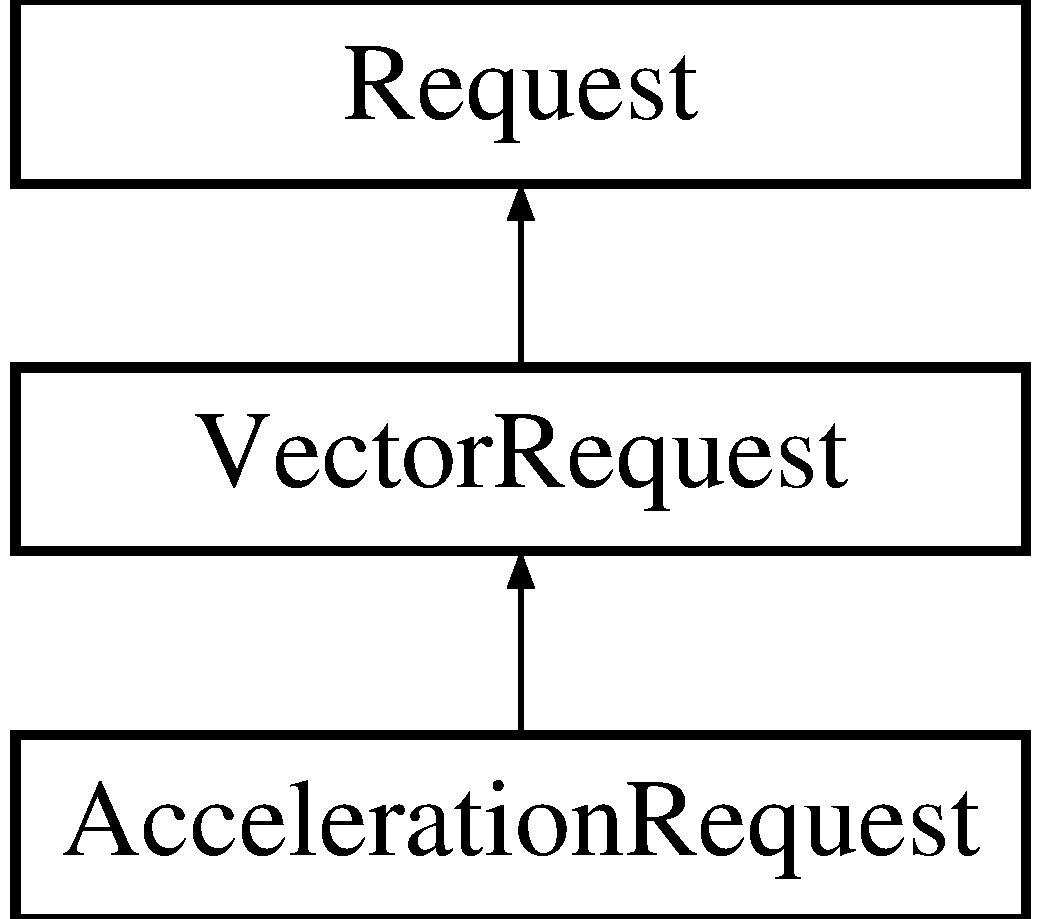
\includegraphics[height=3cm]{class_acceleration_request}
\end{center}
\end{figure}
\subsection*{Public Member Functions}
\begin{CompactItemize}
\item 
\hypertarget{class_acceleration_request_93be16a9111ca256f24919bcfc8a8539}{
\textbf{AccelerationRequest} (Robot \&robot, boost::shared\_\-ptr$<$ Vector3d $>$ requested\_\-vector)}
\label{class_acceleration_request_93be16a9111ca256f24919bcfc8a8539}

\end{CompactItemize}


\subsection{Detailed Description}
An Acceleration \hyperlink{class_request}{Request} is issued by a robot which wants to change its acceleration to a new value. 

Notes: The new acceleration is expressed in terms of the local coordinate system of the robot. This means it has to be transformed before using.

The request cannot be changed after construction. 

Definition at line 23 of file acceleration\_\-request.h.

The documentation for this class was generated from the following file:\begin{CompactItemize}
\item 
src/Requests/acceleration\_\-request.h\end{CompactItemize}

\hypertarget{class_activation_sequence_generator}{
\section{ActivationSequenceGenerator Class Reference}
\label{class_activation_sequence_generator}\index{ActivationSequenceGenerator@{ActivationSequenceGenerator}}
}
Interface for activation sequence generators.  


{\tt \#include $<$activation\_\-sequence\_\-generator.h$>$}

Inheritance diagram for ActivationSequenceGenerator::\begin{figure}[H]
\begin{center}
\leavevmode
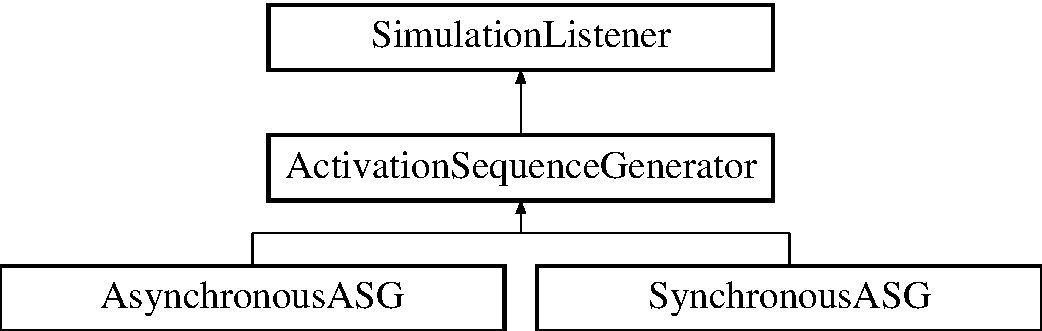
\includegraphics[height=3cm]{class_activation_sequence_generator}
\end{center}
\end{figure}
\subsection*{Public Member Functions}
\begin{CompactItemize}
\item 
virtual void \hyperlink{class_activation_sequence_generator_01592eb2b4293512d2ad00dc4adf0361}{initialize} (const \hyperlink{class_history}{History} \&history, const vector$<$ boost::shared\_\-ptr$<$ Robot $>$ $>$ \&robots)=0
\item 
virtual boost::shared\_\-ptr$<$ Event $>$ \hyperlink{class_activation_sequence_generator_cf20a8caaee580655c57b8843d82d5f5}{get\_\-next\_\-event} ()=0
\item 
virtual int \hyperlink{class_activation_sequence_generator_724cfa2e135813db7becb90af1783050}{get\_\-time\_\-of\_\-next\_\-event} ()=0
\end{CompactItemize}


\subsection{Detailed Description}
Interface for activation sequence generators. 

The activation sequence generator (AGS) decides, according to some user--specified rules, how to time the different events. In other words, it manages the timing of the execution of the robot algorithms.

The \hyperlink{class_activation_sequence_generator}{ActivationSequenceGenerator} class inherits from the \hyperlink{class_simulation_listener}{SimulationListener} interface. 

Definition at line 33 of file activation\_\-sequence\_\-generator.h.

\subsection{Member Function Documentation}
\hypertarget{class_activation_sequence_generator_01592eb2b4293512d2ad00dc4adf0361}{
\index{ActivationSequenceGenerator@{ActivationSequenceGenerator}!initialize@{initialize}}
\index{initialize@{initialize}!ActivationSequenceGenerator@{ActivationSequenceGenerator}}
\subsubsection[initialize]{\setlength{\rightskip}{0pt plus 5cm}virtual void ActivationSequenceGenerator::initialize (const {\bf History} \& {\em history}, \/  const vector$<$ boost::shared\_\-ptr$<$ Robot $>$ $>$ \& {\em robots})\hspace{0.3cm}{\tt  \mbox{[}pure virtual\mbox{]}}}}
\label{class_activation_sequence_generator_01592eb2b4293512d2ad00dc4adf0361}


Initializes the ASG. \begin{Desc}
\item[Parameters:]
\begin{description}
\item[{\em The}]history \end{description}
\end{Desc}


Implemented in \hyperlink{class_asynchronous_a_s_g_6ef9907d9f0043e45cc08a3e0d5178fa}{AsynchronousASG}, and \hyperlink{class_synchronous_a_s_g_05acba7c914bdb8b4080ef763c092993}{SynchronousASG}.\hypertarget{class_activation_sequence_generator_cf20a8caaee580655c57b8843d82d5f5}{
\index{ActivationSequenceGenerator@{ActivationSequenceGenerator}!get\_\-next\_\-event@{get\_\-next\_\-event}}
\index{get\_\-next\_\-event@{get\_\-next\_\-event}!ActivationSequenceGenerator@{ActivationSequenceGenerator}}
\subsubsection[get\_\-next\_\-event]{\setlength{\rightskip}{0pt plus 5cm}virtual boost::shared\_\-ptr$<$Event$>$ ActivationSequenceGenerator::get\_\-next\_\-event ()\hspace{0.3cm}{\tt  \mbox{[}pure virtual\mbox{]}}}}
\label{class_activation_sequence_generator_cf20a8caaee580655c57b8843d82d5f5}


Returns the next event. \begin{Desc}
\item[Returns:]The next event produced by the ASG \end{Desc}


Implemented in \hyperlink{class_asynchronous_a_s_g_cbec6379ed8ba4ea1351e2b1d76b9671}{AsynchronousASG}, and \hyperlink{class_synchronous_a_s_g_05fbdbd3ed9638ab90c3817944fbba95}{SynchronousASG}.\hypertarget{class_activation_sequence_generator_724cfa2e135813db7becb90af1783050}{
\index{ActivationSequenceGenerator@{ActivationSequenceGenerator}!get\_\-time\_\-of\_\-next\_\-event@{get\_\-time\_\-of\_\-next\_\-event}}
\index{get\_\-time\_\-of\_\-next\_\-event@{get\_\-time\_\-of\_\-next\_\-event}!ActivationSequenceGenerator@{ActivationSequenceGenerator}}
\subsubsection[get\_\-time\_\-of\_\-next\_\-event]{\setlength{\rightskip}{0pt plus 5cm}virtual int ActivationSequenceGenerator::get\_\-time\_\-of\_\-next\_\-event ()\hspace{0.3cm}{\tt  \mbox{[}pure virtual\mbox{]}}}}
\label{class_activation_sequence_generator_724cfa2e135813db7becb90af1783050}


Returns the time the next event happens \begin{Desc}
\item[Returns:]Integer representing the next time an event will happen \end{Desc}


Implemented in \hyperlink{class_asynchronous_a_s_g_163256359314a7c69e5cfb684f311201}{AsynchronousASG}, and \hyperlink{class_synchronous_a_s_g_b675d2066e00287119c772b0411531b5}{SynchronousASG}.

The documentation for this class was generated from the following file:\begin{CompactItemize}
\item 
src/ActivationSequenceGenerators/activation\_\-sequence\_\-generator.h\end{CompactItemize}

\hypertarget{class_asynchronous_a_s_g}{
\section{AsynchronousASG Class Reference}
\label{class_asynchronous_a_s_g}\index{AsynchronousASG@{AsynchronousASG}}
}
The asynchronous ASG tries to produce a sequence of events challenging to algorithms developed for the asynchronous time model. Nevertheless it is of course not equivalent to the asynchronous time model.  


{\tt \#include $<$asynchronous\_\-asg.h$>$}

Inheritance diagram for AsynchronousASG::\begin{figure}[H]
\begin{center}
\leavevmode
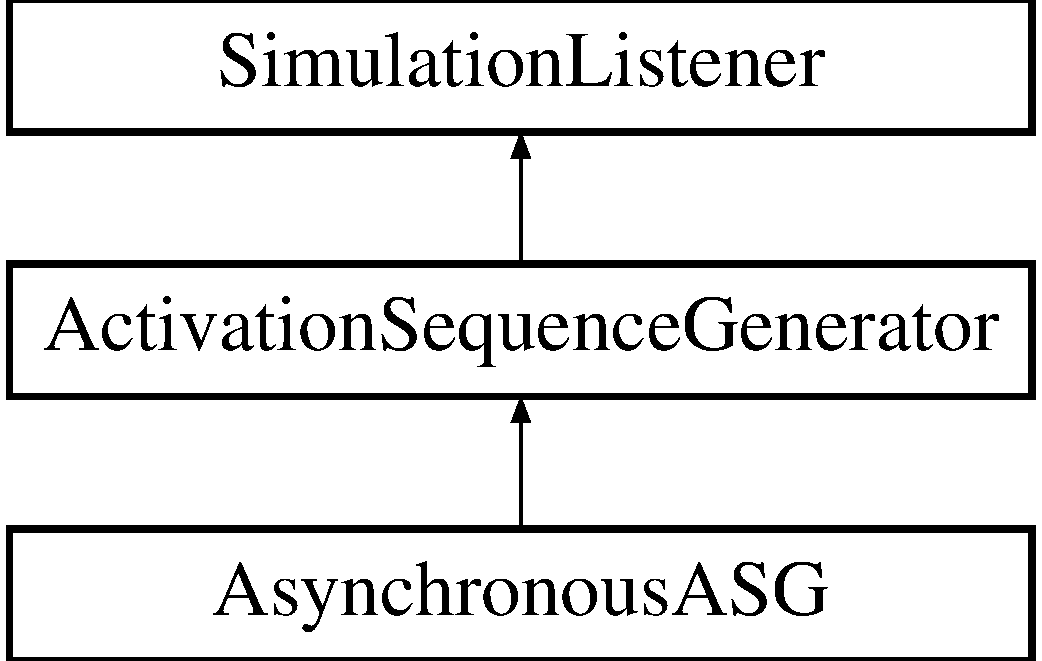
\includegraphics[height=3cm]{class_asynchronous_a_s_g}
\end{center}
\end{figure}
\subsection*{Public Member Functions}
\begin{CompactItemize}
\item 
\hypertarget{class_asynchronous_a_s_g_37707f45332b6e7b68f6d3c9c946cedb}{
\textbf{AsynchronousASG} (unsigned int seed, double participation\_\-probability, double lambda)}
\label{class_asynchronous_a_s_g_37707f45332b6e7b68f6d3c9c946cedb}

\item 
void \hyperlink{class_asynchronous_a_s_g_6ef9907d9f0043e45cc08a3e0d5178fa}{initialize} (const \hyperlink{class_history}{History} \&history, const vector$<$ boost::shared\_\-ptr$<$ Robot $>$ $>$ \&robots)
\item 
boost::shared\_\-ptr$<$ Event $>$ \hyperlink{class_asynchronous_a_s_g_cbec6379ed8ba4ea1351e2b1d76b9671}{get\_\-next\_\-event} ()
\item 
int \hyperlink{class_asynchronous_a_s_g_163256359314a7c69e5cfb684f311201}{get\_\-time\_\-of\_\-next\_\-event} ()
\item 
void \hyperlink{class_asynchronous_a_s_g_159110685ece0b48788dcf9d2c085010}{update} (const \hyperlink{class_world_information}{WorldInformation} \&world\_\-information, boost::shared\_\-ptr$<$ Event $>$ event)
\end{CompactItemize}
\subsection*{Private Member Functions}
\begin{CompactItemize}
\item 
boost::shared\_\-ptr$<$ Event $>$ \hyperlink{class_asynchronous_a_s_g_a8a58e515bb574cc93682d8821682e73}{choose\_\-event\_\-type} ()
\end{CompactItemize}
\subsection*{Private Attributes}
\begin{CompactItemize}
\item 
int \hyperlink{class_asynchronous_a_s_g_2dd36f7979292fdc273a49f0f7fdd6c2}{time\_\-of\_\-next\_\-event\_\-}
\item 
list$<$ boost::shared\_\-ptr$<$ const \hyperlink{class_request}{Request} $>$ $>$ \hyperlink{class_asynchronous_a_s_g_1c00f0cf10435b21e1b3ceb7a1150d6b}{unhandled\_\-request\_\-set\_\-}
\item 
list$<$ boost::shared\_\-ptr$<$ Robot $>$ $>$ \hyperlink{class_asynchronous_a_s_g_1fd277bf5ad58672320c9822197d6109}{looking\_\-robots\_\-}
\item 
list$<$ boost::shared\_\-ptr$<$ Robot $>$ $>$ \hyperlink{class_asynchronous_a_s_g_6e47fd6b84daae67217cb3ca0b09e390}{computing\_\-robots\_\-}
\item 
list$<$ boost::shared\_\-ptr$<$ Robot $>$ $>$ \hyperlink{class_asynchronous_a_s_g_f65d4f1de454809c7e7fcd44699d49e8}{handling\_\-robots\_\-}
\item 
boost::shared\_\-ptr$<$ \hyperlink{class_distribution_generator}{DistributionGenerator} $>$ \hyperlink{class_asynchronous_a_s_g_e5ccdc6beb099e9f243868b31bf66452}{distribution\_\-generator\_\-}
\end{CompactItemize}
\subsection*{Friends}
\begin{CompactItemize}
\item 
class \hyperlink{class_asynchronous_a_s_g_9fbe3b2400008b3dab55bea0e55a5332}{AsynchronousASGTestAccessor}
\end{CompactItemize}


\subsection{Detailed Description}
The asynchronous ASG tries to produce a sequence of events challenging to algorithms developed for the asynchronous time model. Nevertheless it is of course not equivalent to the asynchronous time model. 

The sequence produced by the asynchronous ASG satisfies the following invariants: 1. There are never two events for the same point in time. 2. The order of events for a fixed robot will always be: Look-Compute-HandleRequests 3. In a infinite sequence each robot looks, computes and moves an infinite number of times. 

Definition at line 38 of file asynchronous\_\-asg.h.

\subsection{Member Function Documentation}
\hypertarget{class_asynchronous_a_s_g_6ef9907d9f0043e45cc08a3e0d5178fa}{
\index{AsynchronousASG@{AsynchronousASG}!initialize@{initialize}}
\index{initialize@{initialize}!AsynchronousASG@{AsynchronousASG}}
\subsubsection[initialize]{\setlength{\rightskip}{0pt plus 5cm}void AsynchronousASG::initialize (const {\bf History} \& {\em history}, \/  const vector$<$ boost::shared\_\-ptr$<$ Robot $>$ $>$ \& {\em robots})\hspace{0.3cm}{\tt  \mbox{[}virtual\mbox{]}}}}
\label{class_asynchronous_a_s_g_6ef9907d9f0043e45cc08a3e0d5178fa}


initializes the asynchronous ASG from the given intial world\_\-state. Needs to be called before the ASG is used \begin{Desc}
\item[Parameters:]
\begin{description}
\item[{\em The}]intial world state \end{description}
\end{Desc}


Implements \hyperlink{class_activation_sequence_generator_01592eb2b4293512d2ad00dc4adf0361}{ActivationSequenceGenerator}.

Definition at line 41 of file asynchronous\_\-asg.cc.

References looking\_\-robots\_\-.\hypertarget{class_asynchronous_a_s_g_cbec6379ed8ba4ea1351e2b1d76b9671}{
\index{AsynchronousASG@{AsynchronousASG}!get\_\-next\_\-event@{get\_\-next\_\-event}}
\index{get\_\-next\_\-event@{get\_\-next\_\-event}!AsynchronousASG@{AsynchronousASG}}
\subsubsection[get\_\-next\_\-event]{\setlength{\rightskip}{0pt plus 5cm}boost::shared\_\-ptr$<$ Event $>$ AsynchronousASG::get\_\-next\_\-event ()\hspace{0.3cm}{\tt  \mbox{[}virtual\mbox{]}}}}
\label{class_asynchronous_a_s_g_cbec6379ed8ba4ea1351e2b1d76b9671}


Returns the next event. \begin{Desc}
\item[Returns:]The next event in the sequence. \end{Desc}


Implements \hyperlink{class_activation_sequence_generator_cf20a8caaee580655c57b8843d82d5f5}{ActivationSequenceGenerator}.

Definition at line 49 of file asynchronous\_\-asg.cc.

References choose\_\-event\_\-type(), computing\_\-robots\_\-, distribution\_\-generator\_\-, handling\_\-robots\_\-, looking\_\-robots\_\-, time\_\-of\_\-next\_\-event\_\-, and unhandled\_\-request\_\-set\_\-.\hypertarget{class_asynchronous_a_s_g_163256359314a7c69e5cfb684f311201}{
\index{AsynchronousASG@{AsynchronousASG}!get\_\-time\_\-of\_\-next\_\-event@{get\_\-time\_\-of\_\-next\_\-event}}
\index{get\_\-time\_\-of\_\-next\_\-event@{get\_\-time\_\-of\_\-next\_\-event}!AsynchronousASG@{AsynchronousASG}}
\subsubsection[get\_\-time\_\-of\_\-next\_\-event]{\setlength{\rightskip}{0pt plus 5cm}int AsynchronousASG::get\_\-time\_\-of\_\-next\_\-event ()\hspace{0.3cm}{\tt  \mbox{[}inline, virtual\mbox{]}}}}
\label{class_asynchronous_a_s_g_163256359314a7c69e5cfb684f311201}


Returns the time of the next event. This is computed according to... \begin{Desc}
\item[Returns:]The time of the next event. \end{Desc}


Implements \hyperlink{class_activation_sequence_generator_724cfa2e135813db7becb90af1783050}{ActivationSequenceGenerator}.

Definition at line 66 of file asynchronous\_\-asg.h.

References time\_\-of\_\-next\_\-event\_\-.\hypertarget{class_asynchronous_a_s_g_159110685ece0b48788dcf9d2c085010}{
\index{AsynchronousASG@{AsynchronousASG}!update@{update}}
\index{update@{update}!AsynchronousASG@{AsynchronousASG}}
\subsubsection[update]{\setlength{\rightskip}{0pt plus 5cm}void AsynchronousASG::update (const {\bf WorldInformation} \& {\em world\_\-information}, \/  boost::shared\_\-ptr$<$ Event $>$ {\em event})\hspace{0.3cm}{\tt  \mbox{[}virtual\mbox{]}}}}
\label{class_asynchronous_a_s_g_159110685ece0b48788dcf9d2c085010}


Updates the sequence of events. Ensures that the events for each fixed robot are in the right order \begin{Desc}
\item[Parameters:]
\begin{description}
\item[{\em A}]constant refrence to the newest world information \item[{\em The}]last handled event \end{description}
\end{Desc}


Implements \hyperlink{class_simulation_listener_f1b53fbefce7830648bb059dfd0f18b4}{SimulationListener}.

Definition at line 115 of file asynchronous\_\-asg.cc.

References unhandled\_\-request\_\-set\_\-.\hypertarget{class_asynchronous_a_s_g_a8a58e515bb574cc93682d8821682e73}{
\index{AsynchronousASG@{AsynchronousASG}!choose\_\-event\_\-type@{choose\_\-event\_\-type}}
\index{choose\_\-event\_\-type@{choose\_\-event\_\-type}!AsynchronousASG@{AsynchronousASG}}
\subsubsection[choose\_\-event\_\-type]{\setlength{\rightskip}{0pt plus 5cm}boost::shared\_\-ptr$<$ Event $>$ AsynchronousASG::choose\_\-event\_\-type ()\hspace{0.3cm}{\tt  \mbox{[}private\mbox{]}}}}
\label{class_asynchronous_a_s_g_a8a58e515bb574cc93682d8821682e73}


chooses, which kind of event will happen next. 

Definition at line 125 of file asynchronous\_\-asg.cc.

References computing\_\-robots\_\-, distribution\_\-generator\_\-, handling\_\-robots\_\-, looking\_\-robots\_\-, and time\_\-of\_\-next\_\-event\_\-.

Referenced by get\_\-next\_\-event().

\subsection{Friends And Related Function Documentation}
\hypertarget{class_asynchronous_a_s_g_9fbe3b2400008b3dab55bea0e55a5332}{
\index{AsynchronousASG@{AsynchronousASG}!AsynchronousASGTestAccessor@{AsynchronousASGTestAccessor}}
\index{AsynchronousASGTestAccessor@{AsynchronousASGTestAccessor}!AsynchronousASG@{AsynchronousASG}}
\subsubsection[AsynchronousASGTestAccessor]{\setlength{\rightskip}{0pt plus 5cm}friend class AsynchronousASGTestAccessor\hspace{0.3cm}{\tt  \mbox{[}friend\mbox{]}}}}
\label{class_asynchronous_a_s_g_9fbe3b2400008b3dab55bea0e55a5332}


declare a friend class for doing unit tests with this class. 

Definition at line 43 of file asynchronous\_\-asg.h.

\subsection{Member Data Documentation}
\hypertarget{class_asynchronous_a_s_g_2dd36f7979292fdc273a49f0f7fdd6c2}{
\index{AsynchronousASG@{AsynchronousASG}!time\_\-of\_\-next\_\-event\_\-@{time\_\-of\_\-next\_\-event\_\-}}
\index{time\_\-of\_\-next\_\-event\_\-@{time\_\-of\_\-next\_\-event\_\-}!AsynchronousASG@{AsynchronousASG}}
\subsubsection[time\_\-of\_\-next\_\-event\_\-]{\setlength{\rightskip}{0pt plus 5cm}int {\bf AsynchronousASG::time\_\-of\_\-next\_\-event\_\-}\hspace{0.3cm}{\tt  \mbox{[}private\mbox{]}}}}
\label{class_asynchronous_a_s_g_2dd36f7979292fdc273a49f0f7fdd6c2}


The time the next event will happen. 

Definition at line 86 of file asynchronous\_\-asg.h.

Referenced by choose\_\-event\_\-type(), get\_\-next\_\-event(), and get\_\-time\_\-of\_\-next\_\-event().\hypertarget{class_asynchronous_a_s_g_1c00f0cf10435b21e1b3ceb7a1150d6b}{
\index{AsynchronousASG@{AsynchronousASG}!unhandled\_\-request\_\-set\_\-@{unhandled\_\-request\_\-set\_\-}}
\index{unhandled\_\-request\_\-set\_\-@{unhandled\_\-request\_\-set\_\-}!AsynchronousASG@{AsynchronousASG}}
\subsubsection[unhandled\_\-request\_\-set\_\-]{\setlength{\rightskip}{0pt plus 5cm}list$<$boost::shared\_\-ptr$<$const {\bf Request}$>$ $>$ {\bf AsynchronousASG::unhandled\_\-request\_\-set\_\-}\hspace{0.3cm}{\tt  \mbox{[}private\mbox{]}}}}
\label{class_asynchronous_a_s_g_1c00f0cf10435b21e1b3ceb7a1150d6b}


A set of unhandled requests from some compute events in the past. 

Definition at line 91 of file asynchronous\_\-asg.h.

Referenced by get\_\-next\_\-event(), and update().\hypertarget{class_asynchronous_a_s_g_1fd277bf5ad58672320c9822197d6109}{
\index{AsynchronousASG@{AsynchronousASG}!looking\_\-robots\_\-@{looking\_\-robots\_\-}}
\index{looking\_\-robots\_\-@{looking\_\-robots\_\-}!AsynchronousASG@{AsynchronousASG}}
\subsubsection[looking\_\-robots\_\-]{\setlength{\rightskip}{0pt plus 5cm}list$<$boost::shared\_\-ptr$<$Robot$>$ $>$ {\bf AsynchronousASG::looking\_\-robots\_\-}\hspace{0.3cm}{\tt  \mbox{[}private\mbox{]}}}}
\label{class_asynchronous_a_s_g_1fd277bf5ad58672320c9822197d6109}


The set of all robots which will have a look event as their next event. 

Definition at line 96 of file asynchronous\_\-asg.h.

Referenced by choose\_\-event\_\-type(), get\_\-next\_\-event(), and initialize().\hypertarget{class_asynchronous_a_s_g_6e47fd6b84daae67217cb3ca0b09e390}{
\index{AsynchronousASG@{AsynchronousASG}!computing\_\-robots\_\-@{computing\_\-robots\_\-}}
\index{computing\_\-robots\_\-@{computing\_\-robots\_\-}!AsynchronousASG@{AsynchronousASG}}
\subsubsection[computing\_\-robots\_\-]{\setlength{\rightskip}{0pt plus 5cm}list$<$boost::shared\_\-ptr$<$Robot$>$ $>$ {\bf AsynchronousASG::computing\_\-robots\_\-}\hspace{0.3cm}{\tt  \mbox{[}private\mbox{]}}}}
\label{class_asynchronous_a_s_g_6e47fd6b84daae67217cb3ca0b09e390}


The set of all robots which will have a compute event as their next event. 

Definition at line 101 of file asynchronous\_\-asg.h.

Referenced by choose\_\-event\_\-type(), and get\_\-next\_\-event().\hypertarget{class_asynchronous_a_s_g_f65d4f1de454809c7e7fcd44699d49e8}{
\index{AsynchronousASG@{AsynchronousASG}!handling\_\-robots\_\-@{handling\_\-robots\_\-}}
\index{handling\_\-robots\_\-@{handling\_\-robots\_\-}!AsynchronousASG@{AsynchronousASG}}
\subsubsection[handling\_\-robots\_\-]{\setlength{\rightskip}{0pt plus 5cm}list$<$boost::shared\_\-ptr$<$Robot$>$ $>$ {\bf AsynchronousASG::handling\_\-robots\_\-}\hspace{0.3cm}{\tt  \mbox{[}private\mbox{]}}}}
\label{class_asynchronous_a_s_g_f65d4f1de454809c7e7fcd44699d49e8}


The set of all robots which will have handle requests event as their next event. 

Definition at line 106 of file asynchronous\_\-asg.h.

Referenced by choose\_\-event\_\-type(), and get\_\-next\_\-event().\hypertarget{class_asynchronous_a_s_g_e5ccdc6beb099e9f243868b31bf66452}{
\index{AsynchronousASG@{AsynchronousASG}!distribution\_\-generator\_\-@{distribution\_\-generator\_\-}}
\index{distribution\_\-generator\_\-@{distribution\_\-generator\_\-}!AsynchronousASG@{AsynchronousASG}}
\subsubsection[distribution\_\-generator\_\-]{\setlength{\rightskip}{0pt plus 5cm}boost::shared\_\-ptr$<${\bf DistributionGenerator}$>$ {\bf AsynchronousASG::distribution\_\-generator\_\-}\hspace{0.3cm}{\tt  \mbox{[}private\mbox{]}}}}
\label{class_asynchronous_a_s_g_e5ccdc6beb099e9f243868b31bf66452}


a source of randomness 

Definition at line 111 of file asynchronous\_\-asg.h.

Referenced by choose\_\-event\_\-type(), and get\_\-next\_\-event().

The documentation for this class was generated from the following files:\begin{CompactItemize}
\item 
src/ActivationSequenceGenerators/asynchronous\_\-asg.h\item 
src/ActivationSequenceGenerators/asynchronous\_\-asg.cc\end{CompactItemize}

\hypertarget{class_box}{
\section{Box Class Reference}
\label{class_box}\index{Box@{Box}}
}
Denotes an box-obstacle.  


{\tt \#include $<$box.h$>$}

Inheritance diagram for Box::\begin{figure}[H]
\begin{center}
\leavevmode
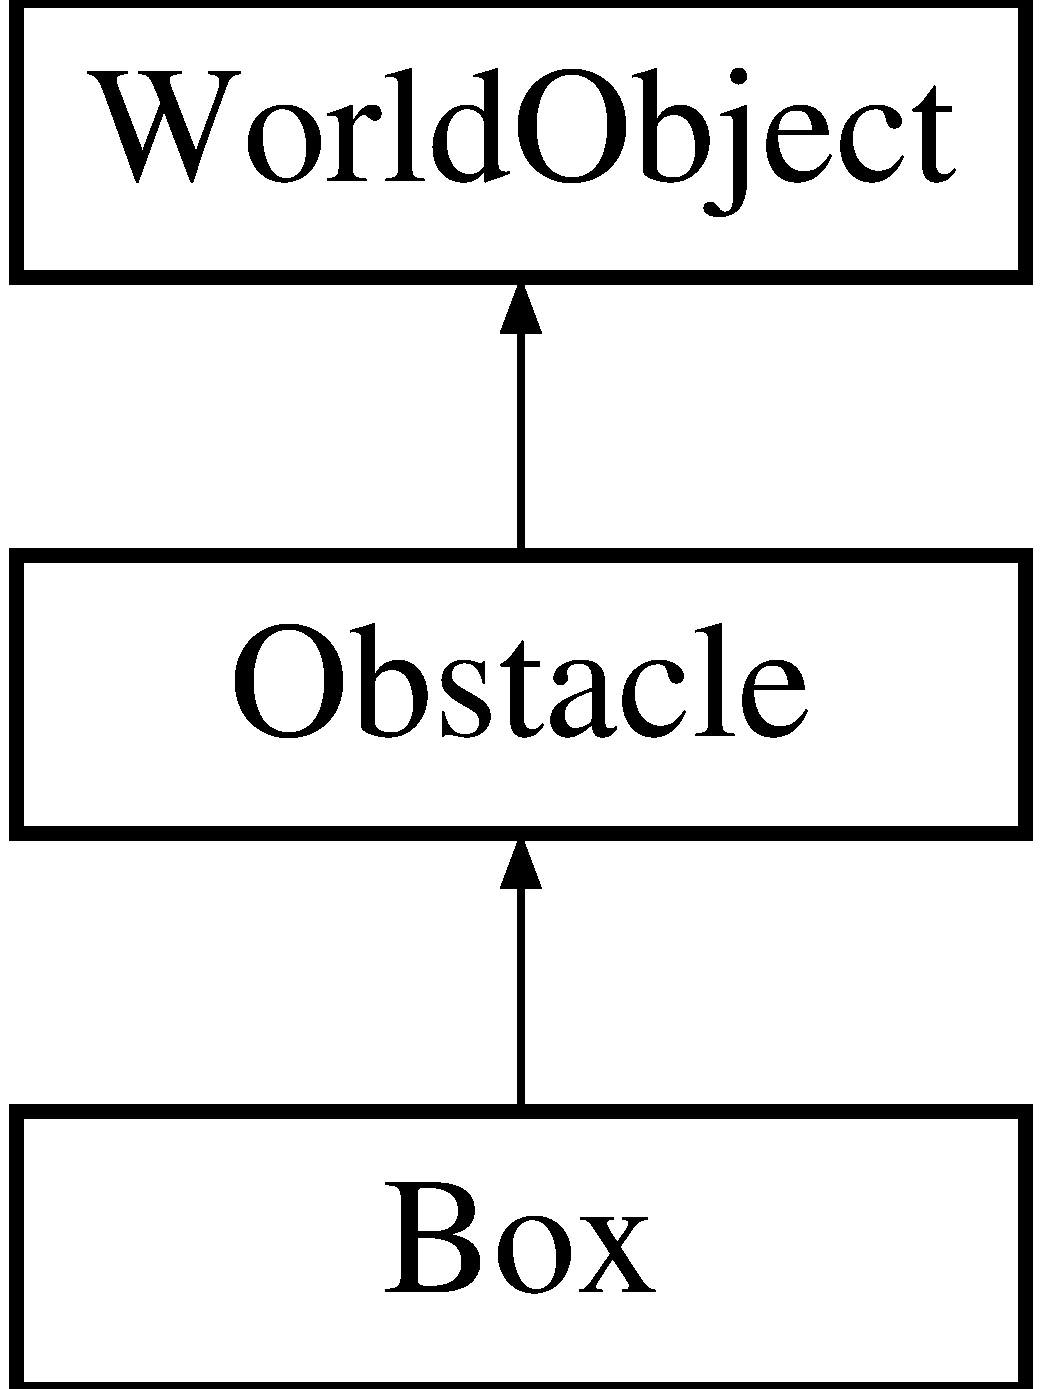
\includegraphics[height=3cm]{class_box}
\end{center}
\end{figure}
\subsection*{Public Member Functions}
\begin{CompactItemize}
\item 
\hypertarget{class_box_24307773a7e83c489ab732148ae8dc8a}{
\textbf{Box} (boost::shared\_\-ptr$<$ \hyperlink{class_identifier}{Identifier} $>$ id, boost::shared\_\-ptr$<$ Vector3d $>$ position, double depth, double width, double height)}
\label{class_box_24307773a7e83c489ab732148ae8dc8a}

\item 
\hypertarget{class_box_44331abde2dcbba2f0293c60f87cbdb8}{
\textbf{Box} (boost::shared\_\-ptr$<$ \hyperlink{class_identifier}{Identifier} $>$ id, boost::shared\_\-ptr$<$ Vector3d $>$ position, boost::shared\_\-ptr$<$ \hyperlink{class_marker_information}{MarkerInformation} $>$ marker\_\-information, double depth, double width, double height)}
\label{class_box_44331abde2dcbba2f0293c60f87cbdb8}

\item 
double \hyperlink{class_box_8b436da1c22ee2335d692fe44c53ce90}{height} () const 
\item 
void \hyperlink{class_box_98acafd52d9a5596a6f6d1b87918fd2d}{set\_\-height} (double new\_\-height)
\item 
double \hyperlink{class_box_10dbd2cb5f3c37ca36792d4a1e34240d}{depth} () const 
\item 
void \hyperlink{class_box_8449b2ab9741bd60c24f15de96567a77}{set\_\-depth} (double new\_\-depth)
\item 
double \hyperlink{class_box_cceec88bdb7cccd65b090837e919982c}{width} () const 
\item 
void \hyperlink{class_box_c681f5c0251287c23b004e7e13246581}{set\_\-width} (double new\_\-width)
\item 
bool \hyperlink{class_box_3ef2a0b5fc2bed2036c5fc6e350335f2}{contains\_\-point} (boost::shared\_\-ptr$<$ Vector3d $>$ point) const 
\item 
virtual boost::shared\_\-ptr$<$ \hyperlink{class_world_object}{WorldObject} $>$ \hyperlink{class_box_06c27f9a07a6ba9e87aa0c2e57237b5c}{clone} () const 
\end{CompactItemize}
\subsection*{Private Attributes}
\begin{CompactItemize}
\item 
\hypertarget{class_box_4a10d30962d726db33010380ff817ba7}{
double \textbf{depth\_\-}}
\label{class_box_4a10d30962d726db33010380ff817ba7}

\item 
\hypertarget{class_box_ae8acc7abfcd89d46fcb01562dfc53b0}{
double \textbf{width\_\-}}
\label{class_box_ae8acc7abfcd89d46fcb01562dfc53b0}

\item 
\hypertarget{class_box_9b372de7550463c8bad45d61a23bfe5a}{
double \textbf{height\_\-}}
\label{class_box_9b372de7550463c8bad45d61a23bfe5a}

\end{CompactItemize}


\subsection{Detailed Description}
Denotes an box-obstacle. 

\begin{Desc}
\item[Author:]Martina Hüllmann \end{Desc}


Definition at line 14 of file box.h.

\subsection{Member Function Documentation}
\hypertarget{class_box_8b436da1c22ee2335d692fe44c53ce90}{
\index{Box@{Box}!height@{height}}
\index{height@{height}!Box@{Box}}
\subsubsection[height]{\setlength{\rightskip}{0pt plus 5cm}double Box::height () const}}
\label{class_box_8b436da1c22ee2335d692fe44c53ce90}


Returns the length of the box. \begin{Desc}
\item[Returns:]Length of the box. \end{Desc}


Definition at line 22 of file box.cc.

Referenced by Octree::determine\_\-obstacle\_\-max\_\-size().\hypertarget{class_box_98acafd52d9a5596a6f6d1b87918fd2d}{
\index{Box@{Box}!set\_\-height@{set\_\-height}}
\index{set\_\-height@{set\_\-height}!Box@{Box}}
\subsubsection[set\_\-height]{\setlength{\rightskip}{0pt plus 5cm}void Box::set\_\-height (double {\em new\_\-height})}}
\label{class_box_98acafd52d9a5596a6f6d1b87918fd2d}


Sets the height of the box to the given value. \begin{Desc}
\item[Parameters:]
\begin{description}
\item[{\em New}]height of the box. \end{description}
\end{Desc}


Definition at line 26 of file box.cc.\hypertarget{class_box_10dbd2cb5f3c37ca36792d4a1e34240d}{
\index{Box@{Box}!depth@{depth}}
\index{depth@{depth}!Box@{Box}}
\subsubsection[depth]{\setlength{\rightskip}{0pt plus 5cm}double Box::depth () const}}
\label{class_box_10dbd2cb5f3c37ca36792d4a1e34240d}


Returns the depth of the box. \begin{Desc}
\item[Returns:]Depth of the box. \end{Desc}


Definition at line 30 of file box.cc.

Referenced by Octree::determine\_\-obstacle\_\-max\_\-size().\hypertarget{class_box_8449b2ab9741bd60c24f15de96567a77}{
\index{Box@{Box}!set\_\-depth@{set\_\-depth}}
\index{set\_\-depth@{set\_\-depth}!Box@{Box}}
\subsubsection[set\_\-depth]{\setlength{\rightskip}{0pt plus 5cm}void Box::set\_\-depth (double {\em new\_\-depth})}}
\label{class_box_8449b2ab9741bd60c24f15de96567a77}


Sets the depth of the box to the given value. \begin{Desc}
\item[Parameters:]
\begin{description}
\item[{\em New}]depth of the box. \end{description}
\end{Desc}


Definition at line 34 of file box.cc.\hypertarget{class_box_cceec88bdb7cccd65b090837e919982c}{
\index{Box@{Box}!width@{width}}
\index{width@{width}!Box@{Box}}
\subsubsection[width]{\setlength{\rightskip}{0pt plus 5cm}double Box::width () const}}
\label{class_box_cceec88bdb7cccd65b090837e919982c}


Returns the width of the box. \begin{Desc}
\item[Returns:]Width of the box. \end{Desc}


Definition at line 38 of file box.cc.

Referenced by Octree::determine\_\-obstacle\_\-max\_\-size().\hypertarget{class_box_c681f5c0251287c23b004e7e13246581}{
\index{Box@{Box}!set\_\-width@{set\_\-width}}
\index{set\_\-width@{set\_\-width}!Box@{Box}}
\subsubsection[set\_\-width]{\setlength{\rightskip}{0pt plus 5cm}void Box::set\_\-width (double {\em new\_\-width})}}
\label{class_box_c681f5c0251287c23b004e7e13246581}


Sets the width of the box to the given value. \begin{Desc}
\item[Parameters:]
\begin{description}
\item[{\em New}]width of the box. \end{description}
\end{Desc}


Definition at line 42 of file box.cc.\hypertarget{class_box_3ef2a0b5fc2bed2036c5fc6e350335f2}{
\index{Box@{Box}!contains\_\-point@{contains\_\-point}}
\index{contains\_\-point@{contains\_\-point}!Box@{Box}}
\subsubsection[contains\_\-point]{\setlength{\rightskip}{0pt plus 5cm}bool Box::contains\_\-point (boost::shared\_\-ptr$<$ Vector3d $>$ {\em point}) const}}
\label{class_box_3ef2a0b5fc2bed2036c5fc6e350335f2}


Checks whether the given point is contained in the obstacle. \begin{Desc}
\item[Parameters:]
\begin{description}
\item[{\em Pointer}]to vector of point to check whether it's contained in the obstacle. \end{description}
\end{Desc}


Definition at line 51 of file box.cc.\hypertarget{class_box_06c27f9a07a6ba9e87aa0c2e57237b5c}{
\index{Box@{Box}!clone@{clone}}
\index{clone@{clone}!Box@{Box}}
\subsubsection[clone]{\setlength{\rightskip}{0pt plus 5cm}boost::shared\_\-ptr$<$ {\bf WorldObject} $>$ Box::clone () const\hspace{0.3cm}{\tt  \mbox{[}virtual\mbox{]}}}}
\label{class_box_06c27f9a07a6ba9e87aa0c2e57237b5c}


Clones this object and returns a shared ptr to the cloned object. typeid($\ast$this) == typeid($\ast$clone) \begin{Desc}
\item[Returns:]shared ptr to the cloned object \end{Desc}


Reimplemented from \hyperlink{class_world_object_dba468299ce77ce5781e60081bf44b14}{WorldObject}.

Definition at line 46 of file box.cc.

The documentation for this class was generated from the following files:\begin{CompactItemize}
\item 
src/Model/box.h\item 
src/Model/box.cc\end{CompactItemize}

\hypertarget{class_box_identifier}{
\section{BoxIdentifier Class Reference}
\label{class_box_identifier}\index{BoxIdentifier@{BoxIdentifier}}
}
Denote ID's of boxes.  


{\tt \#include $<$box\_\-identifier.h$>$}

Inheritance diagram for BoxIdentifier::\begin{figure}[H]
\begin{center}
\leavevmode
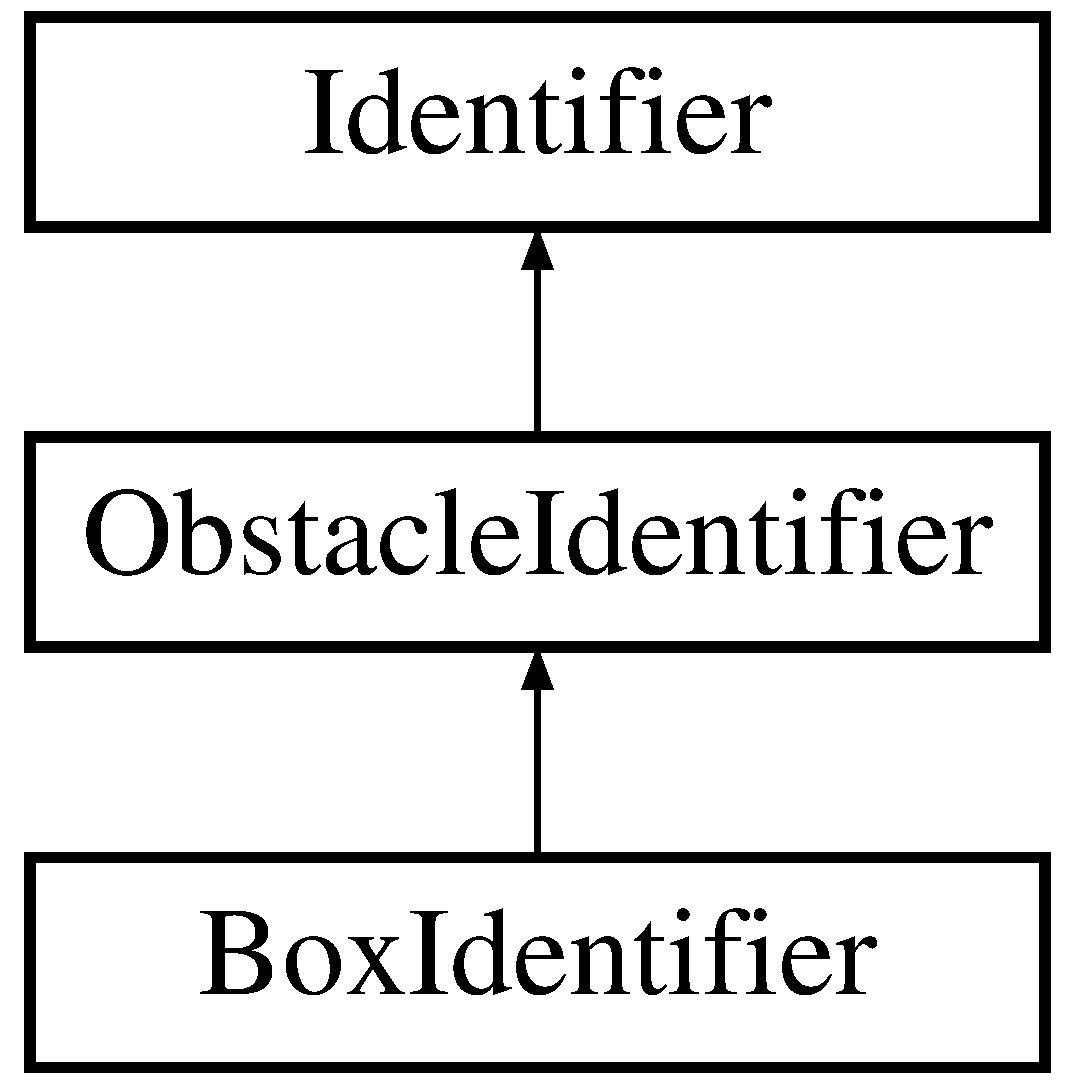
\includegraphics[height=3cm]{class_box_identifier}
\end{center}
\end{figure}
\subsection*{Public Member Functions}
\begin{CompactItemize}
\item 
\hypertarget{class_box_identifier_b8201316d04af5dc947777677a68f53f}{
virtual boost::shared\_\-ptr$<$ \hyperlink{class_identifier}{Identifier} $>$ \textbf{clone} () const }
\label{class_box_identifier_b8201316d04af5dc947777677a68f53f}

\end{CompactItemize}
\subsection*{Protected Member Functions}
\begin{CompactItemize}
\item 
\hypertarget{class_box_identifier_da0b4ca636866324333b732697963d20}{
\textbf{BoxIdentifier} (std::size\_\-t id)}
\label{class_box_identifier_da0b4ca636866324333b732697963d20}

\end{CompactItemize}
\subsection*{Friends}
\begin{CompactItemize}
\item 
\hypertarget{class_box_identifier_6433c824d5e64fc5b3635b2a0f2af16c}{
class \textbf{SimpleWorldFixture}}
\label{class_box_identifier_6433c824d5e64fc5b3635b2a0f2af16c}

\end{CompactItemize}


\subsection{Detailed Description}
Denote ID's of boxes. 

\begin{Desc}
\item[Author:]Martina Hüllmann \end{Desc}


Definition at line 12 of file box\_\-identifier.h.

The documentation for this class was generated from the following files:\begin{CompactItemize}
\item 
src/Model/box\_\-identifier.h\item 
src/Model/box\_\-identifier.cc\end{CompactItemize}

\hypertarget{class_chain_view}{
\section{ChainView Class Reference}
\label{class_chain_view}\index{ChainView@{ChainView}}
}
\hyperlink{class_view}{View} model of the robot chain algorithm.  


{\tt \#include $<$chain\_\-view.h$>$}

Inheritance diagram for ChainView::\begin{figure}[H]
\begin{center}
\leavevmode
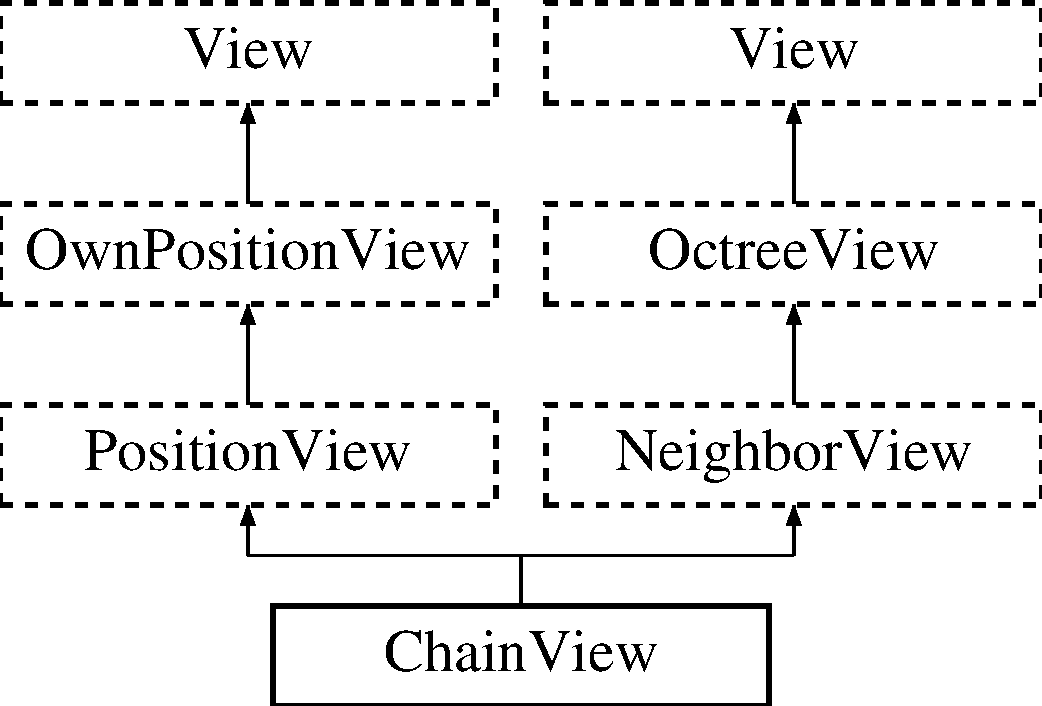
\includegraphics[height=4cm]{class_chain_view}
\end{center}
\end{figure}
\subsection*{Public Member Functions}
\begin{CompactItemize}
\item 
\hypertarget{class_chain_view_c234fecf204d749c81737a71a51f98db}{
\textbf{ChainView} (unsigned k)}
\label{class_chain_view_c234fecf204d749c81737a71a51f98db}

\end{CompactItemize}


\subsection{Detailed Description}
\hyperlink{class_view}{View} model of the robot chain algorithm. 

Assigning this class to a Robot corresponds to the robot chain view model, i.e. every Robot can see k neighbor Robots position. Besides this no more information is visible.

\begin{Desc}
\item[See also:]\href{https://wiki.math.uni-paderborn.de/pg-schwarm/StartSeite/AK/Szenarien}{\tt https://wiki.math.uni-paderborn.de/pg-schwarm/StartSeite/AK/Szenarien} \end{Desc}


Definition at line 25 of file chain\_\-view.h.

The documentation for this class was generated from the following files:\begin{CompactItemize}
\item 
src/Views/chain\_\-view.h\item 
src/Views/chain\_\-view.cc\end{CompactItemize}

\hypertarget{class_cog_view}{
\section{CogView Class Reference}
\label{class_cog_view}\index{CogView@{CogView}}
}
\hyperlink{class_view}{View} model of the classic CenterOfGravity algorithm.  


{\tt \#include $<$cog\_\-view.h$>$}

Inheritance diagram for CogView::\begin{figure}[H]
\begin{center}
\leavevmode
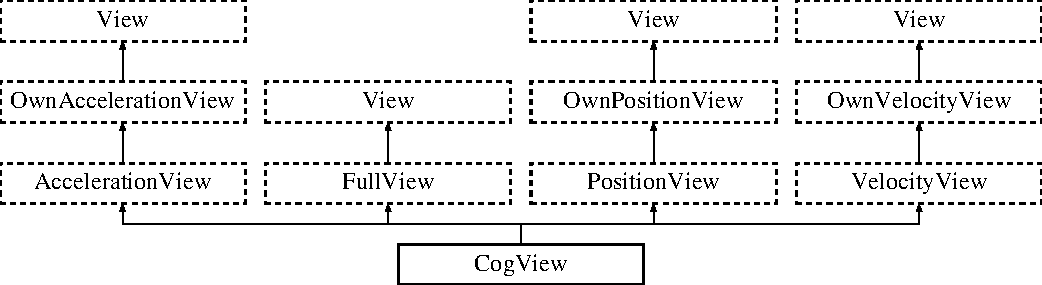
\includegraphics[height=3.83562cm]{class_cog_view}
\end{center}
\end{figure}


\subsection{Detailed Description}
\hyperlink{class_view}{View} model of the classic CenterOfGravity algorithm. 

Assigning this class to a Robot corresponds to the COG view model, i.e. every Robot can see every other Robots position, velocity and acceleration. The coordinate-system and id of each Robot is not visible.

\begin{Desc}
\item[See also:]\href{https://wiki.math.uni-paderborn.de/pg-schwarm/StartSeite/AK/Szenarien}{\tt https://wiki.math.uni-paderborn.de/pg-schwarm/StartSeite/AK/Szenarien} \end{Desc}


Definition at line 27 of file cog\_\-view.h.

The documentation for this class was generated from the following files:\begin{CompactItemize}
\item 
src/Views/cog\_\-view.h\item 
src/Views/cog\_\-view.cc\end{CompactItemize}

\hypertarget{class_compute_event}{
\section{ComputeEvent Class Reference}
\label{class_compute_event}\index{ComputeEvent@{ComputeEvent}}
}
A \hyperlink{class_compute_event}{ComputeEvent} is an event which causes a subset of the robots to calculate new requests.  


{\tt \#include $<$compute\_\-event.h$>$}

Inheritance diagram for ComputeEvent::\begin{figure}[H]
\begin{center}
\leavevmode
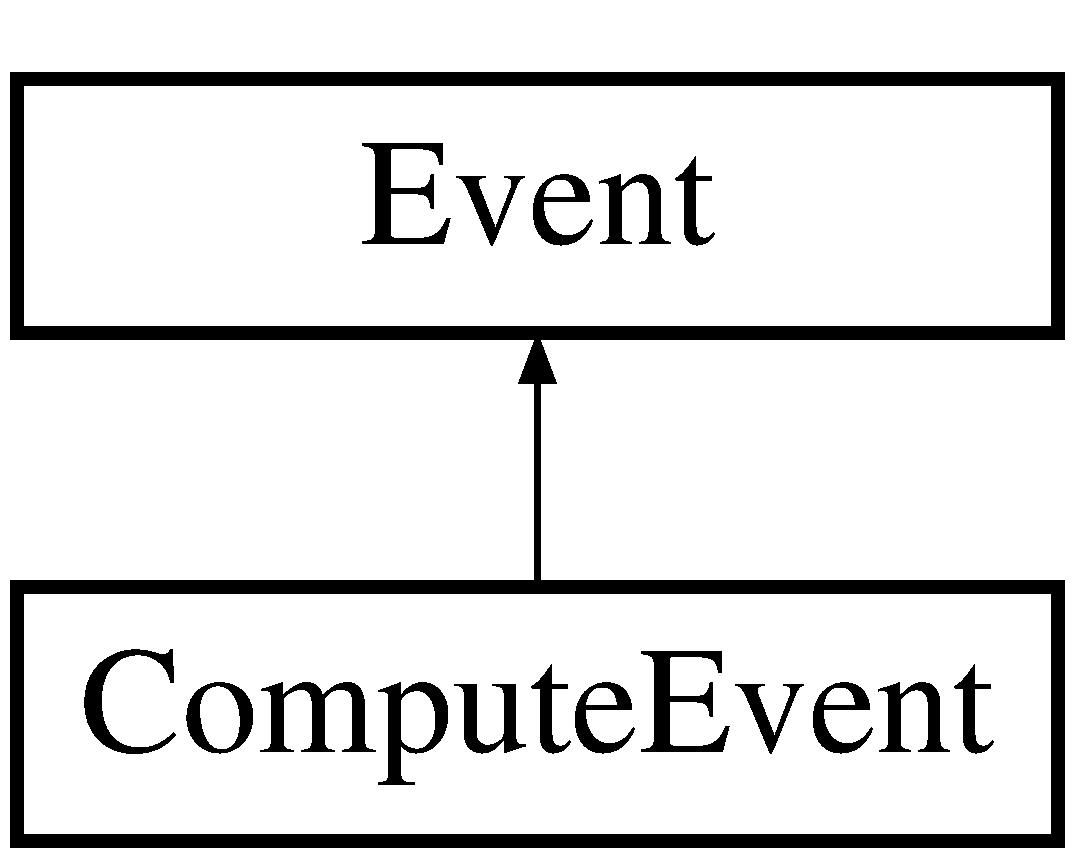
\includegraphics[height=2cm]{class_compute_event}
\end{center}
\end{figure}
\subsection*{Public Member Functions}
\begin{CompactItemize}
\item 
\hypertarget{class_compute_event_4dc6eee8abfa25658b1cf2b9661ff540}{
\textbf{ComputeEvent} (int time)}
\label{class_compute_event_4dc6eee8abfa25658b1cf2b9661ff540}

\item 
void \hyperlink{class_compute_event_7268b70a949c8e9fb1116a1ced0e0071}{add\_\-to\_\-robot\_\-subset} (boost::shared\_\-ptr$<$ Robot $>$ new\_\-robot)
\item 
const vector$<$ boost::shared\_\-ptr$<$ Robot $>$ $>$ \& \hyperlink{class_compute_event_ab47f53949412a2ae5f182206aebf438}{robot\_\-subset} () const 
\item 
void \hyperlink{class_compute_event_97884cf9d3eebb04629883c239a7ecfa}{add\_\-to\_\-requests} (boost::shared\_\-ptr$<$ const \hyperlink{class_request}{Request} $>$ new\_\-request)
\item 
const vector$<$ boost::shared\_\-ptr$<$ const \hyperlink{class_request}{Request} $>$ $>$ \& \hyperlink{class_compute_event_0e685c0e02288e058d59f7eeff83b74d}{requests} () const 
\end{CompactItemize}
\subsection*{Private Attributes}
\begin{CompactItemize}
\item 
vector$<$ boost::shared\_\-ptr$<$ Robot $>$ $>$ \hyperlink{class_compute_event_2dbee5c3df3a079df940e2992b0afc30}{robot\_\-subset\_\-}
\item 
vector$<$ boost::shared\_\-ptr$<$ const \hyperlink{class_request}{Request} $>$ $>$ \hyperlink{class_compute_event_31c8515c8d6eeddecf1111fc8fd0ba67}{requests\_\-}
\end{CompactItemize}


\subsection{Detailed Description}
A \hyperlink{class_compute_event}{ComputeEvent} is an event which causes a subset of the robots to calculate new requests. 

Definition at line 24 of file compute\_\-event.h.

\subsection{Member Function Documentation}
\hypertarget{class_compute_event_7268b70a949c8e9fb1116a1ced0e0071}{
\index{ComputeEvent@{ComputeEvent}!add\_\-to\_\-robot\_\-subset@{add\_\-to\_\-robot\_\-subset}}
\index{add\_\-to\_\-robot\_\-subset@{add\_\-to\_\-robot\_\-subset}!ComputeEvent@{ComputeEvent}}
\subsubsection[add\_\-to\_\-robot\_\-subset]{\setlength{\rightskip}{0pt plus 5cm}void ComputeEvent::add\_\-to\_\-robot\_\-subset (boost::shared\_\-ptr$<$ Robot $>$ {\em new\_\-robot})}}
\label{class_compute_event_7268b70a949c8e9fb1116a1ced0e0071}


Adds a new robot to the subset of robots in the event. \begin{Desc}
\item[Parameters:]
\begin{description}
\item[{\em A}]shared pointer to the new robot. \end{description}
\end{Desc}


Definition at line 10 of file compute\_\-event.cc.

References robot\_\-subset\_\-.

Referenced by SynchronousASG::get\_\-next\_\-event().\hypertarget{class_compute_event_ab47f53949412a2ae5f182206aebf438}{
\index{ComputeEvent@{ComputeEvent}!robot\_\-subset@{robot\_\-subset}}
\index{robot\_\-subset@{robot\_\-subset}!ComputeEvent@{ComputeEvent}}
\subsubsection[robot\_\-subset]{\setlength{\rightskip}{0pt plus 5cm}const vector$<$ boost::shared\_\-ptr$<$ Robot $>$ $>$ \& ComputeEvent::robot\_\-subset () const}}
\label{class_compute_event_ab47f53949412a2ae5f182206aebf438}


Returns a constant reference to the robot subset. \begin{Desc}
\item[Returns:]A constant reference to the robot subset. \end{Desc}


Definition at line 15 of file compute\_\-event.cc.

References robot\_\-subset\_\-.\hypertarget{class_compute_event_97884cf9d3eebb04629883c239a7ecfa}{
\index{ComputeEvent@{ComputeEvent}!add\_\-to\_\-requests@{add\_\-to\_\-requests}}
\index{add\_\-to\_\-requests@{add\_\-to\_\-requests}!ComputeEvent@{ComputeEvent}}
\subsubsection[add\_\-to\_\-requests]{\setlength{\rightskip}{0pt plus 5cm}void ComputeEvent::add\_\-to\_\-requests (boost::shared\_\-ptr$<$ const {\bf Request} $>$ {\em new\_\-request})}}
\label{class_compute_event_97884cf9d3eebb04629883c239a7ecfa}


Adds a new request to the set of requests. \begin{Desc}
\item[Parameters:]
\begin{description}
\item[{\em A}]shared pointer to the new request. \end{description}
\end{Desc}


Definition at line 19 of file compute\_\-event.cc.

References requests\_\-.\hypertarget{class_compute_event_0e685c0e02288e058d59f7eeff83b74d}{
\index{ComputeEvent@{ComputeEvent}!requests@{requests}}
\index{requests@{requests}!ComputeEvent@{ComputeEvent}}
\subsubsection[requests]{\setlength{\rightskip}{0pt plus 5cm}const vector$<$ boost::shared\_\-ptr$<$ const {\bf Request} $>$ $>$ \& ComputeEvent::requests () const}}
\label{class_compute_event_0e685c0e02288e058d59f7eeff83b74d}


Returns a constant reference to the set of requests. \begin{Desc}
\item[Returns:]A constant reference to the set of requests. \end{Desc}


Definition at line 23 of file compute\_\-event.cc.

References requests\_\-.

Referenced by SynchronousASG::update().

\subsection{Member Data Documentation}
\hypertarget{class_compute_event_2dbee5c3df3a079df940e2992b0afc30}{
\index{ComputeEvent@{ComputeEvent}!robot\_\-subset\_\-@{robot\_\-subset\_\-}}
\index{robot\_\-subset\_\-@{robot\_\-subset\_\-}!ComputeEvent@{ComputeEvent}}
\subsubsection[robot\_\-subset\_\-]{\setlength{\rightskip}{0pt plus 5cm}vector$<$boost::shared\_\-ptr$<$Robot$>$ $>$ {\bf ComputeEvent::robot\_\-subset\_\-}\hspace{0.3cm}{\tt  \mbox{[}private\mbox{]}}}}
\label{class_compute_event_2dbee5c3df3a079df940e2992b0afc30}


The robot subset for this event. 

Definition at line 57 of file compute\_\-event.h.

Referenced by add\_\-to\_\-robot\_\-subset(), and robot\_\-subset().\hypertarget{class_compute_event_31c8515c8d6eeddecf1111fc8fd0ba67}{
\index{ComputeEvent@{ComputeEvent}!requests\_\-@{requests\_\-}}
\index{requests\_\-@{requests\_\-}!ComputeEvent@{ComputeEvent}}
\subsubsection[requests\_\-]{\setlength{\rightskip}{0pt plus 5cm}vector$<$boost::shared\_\-ptr$<$const {\bf Request}$>$ $>$ {\bf ComputeEvent::requests\_\-}\hspace{0.3cm}{\tt  \mbox{[}private\mbox{]}}}}
\label{class_compute_event_31c8515c8d6eeddecf1111fc8fd0ba67}


The set of resulting requests 

Definition at line 62 of file compute\_\-event.h.

Referenced by add\_\-to\_\-requests(), and requests().

The documentation for this class was generated from the following files:\begin{CompactItemize}
\item 
src/Events/compute\_\-event.h\item 
src/Events/compute\_\-event.cc\end{CompactItemize}

\hypertarget{class_distribution_generator}{
\section{DistributionGenerator Class Reference}
\label{class_distribution_generator}\index{DistributionGenerator@{DistributionGenerator}}
}
{\tt \#include $<$distribution\_\-generator.h$>$}

\subsection*{Public Member Functions}
\begin{CompactItemize}
\item 
void \hyperlink{class_distribution_generator_fd5fdeedbf8015f742a1d9a4557ce50e}{init\_\-uniform} (int min, int max)
\item 
int \hyperlink{class_distribution_generator_60f7610a91c00ff1919613088c7aff59}{get\_\-value\_\-uniform} ()
\item 
void \hyperlink{class_distribution_generator_91bfbf1fa31540fdccb5fccb98abbf9a}{init\_\-normal} (double mean, double sigma)
\item 
double \hyperlink{class_distribution_generator_cee20f8384e79b351040f9d864750569}{get\_\-value\_\-normal} ()
\item 
void \hyperlink{class_distribution_generator_00f450f4a649e3a5c53d9cdebf160e67}{init\_\-bernoulli} (double probability)
\item 
bool \hyperlink{class_distribution_generator_f9be2ca79fea37085900802673d9c16a}{get\_\-value\_\-bernoulli} ()
\item 
void \hyperlink{class_distribution_generator_5204a1fa18cf090b2fe3891d4d3f7a07}{init\_\-exponential} (double lambda)
\item 
double \hyperlink{class_distribution_generator_217a1822a0f49680cbc8a32bb75ba687}{get\_\-value\_\-exponential} ()
\item 
void \hyperlink{class_distribution_generator_2b293a6d907be3c3d182a1d8dc234fdf}{init\_\-uniform\_\-real} (double min, double max)
\item 
double \hyperlink{class_distribution_generator_0d7089a0e10b8fad8a70b2e1c8b23ba6}{get\_\-value\_\-uniform\_\-real} ()
\item 
void \hyperlink{class_distribution_generator_66a05089faa08bf8939496f87c2672ef}{init\_\-uniform\_\-on\_\-sphere} (int dim)
\item 
std::vector$<$ double $>$ \hyperlink{class_distribution_generator_e11f8754b4a01555fcf929ac58179021}{get\_\-value\_\-uniform\_\-on\_\-sphere} ()
\item 
Vector3d \hyperlink{class_distribution_generator_8162739d29e15e6a7ffacd2e66954ae6}{get\_\-value\_\-uniform\_\-on\_\-sphere\_\-3d} ()
\item 
void \hyperlink{class_distribution_generator_0d1d61ff597511560c3e48a5ee7ccee9}{set\_\-seed} (unsigned int seed)
\item 
\hyperlink{class_distribution_generator_2472817069deda51980e39d36d635991}{DistributionGenerator} (unsigned int seed)
\end{CompactItemize}
\subsection*{Private Attributes}
\begin{CompactItemize}
\item 
\hypertarget{class_distribution_generator_7631897310c1faaf465efe831e6d38b0}{
boost::shared\_\-ptr$<$ boost::variate\_\-generator$<$ boost::mt19937 \&, boost::uniform\_\-int$<$$>$ $>$ $>$ \textbf{gen\_\-uniform\_\-int\_\-}}
\label{class_distribution_generator_7631897310c1faaf465efe831e6d38b0}

\item 
\hypertarget{class_distribution_generator_d3ba3b04de2853ff8e7a30dfcef6d081}{
boost::shared\_\-ptr$<$ boost::variate\_\-generator$<$ boost::mt19937 \&, boost::normal\_\-distribution$<$$>$ $>$ $>$ \textbf{gen\_\-normal\_\-}}
\label{class_distribution_generator_d3ba3b04de2853ff8e7a30dfcef6d081}

\item 
\hypertarget{class_distribution_generator_ee0c415f08c1fae8dee3ca10c23f9b96}{
boost::shared\_\-ptr$<$ boost::variate\_\-generator$<$ boost::mt19937 \&, boost::bernoulli\_\-distribution$<$$>$ $>$ $>$ \textbf{gen\_\-bernoulli\_\-}}
\label{class_distribution_generator_ee0c415f08c1fae8dee3ca10c23f9b96}

\item 
\hypertarget{class_distribution_generator_d4807485cfe60d54b47a14e2115987c9}{
boost::shared\_\-ptr$<$ boost::variate\_\-generator$<$ boost::mt19937 \&, boost::exponential\_\-distribution$<$$>$ $>$ $>$ \textbf{gen\_\-exponential\_\-}}
\label{class_distribution_generator_d4807485cfe60d54b47a14e2115987c9}

\item 
\hypertarget{class_distribution_generator_0910c15a4e74475eff33ff5b82a2ac8d}{
boost::shared\_\-ptr$<$ boost::variate\_\-generator$<$ boost::mt19937 \&, boost::uniform\_\-real$<$$>$ $>$ $>$ \textbf{gen\_\-uniform\_\-real\_\-}}
\label{class_distribution_generator_0910c15a4e74475eff33ff5b82a2ac8d}

\item 
\hypertarget{class_distribution_generator_e0b00c288f47cc07973ac3c3d4a23975}{
boost::shared\_\-ptr$<$ boost::variate\_\-generator$<$ boost::mt19937 \&, boost::uniform\_\-on\_\-sphere$<$$>$ $>$ $>$ \textbf{gen\_\-uniform\_\-on\_\-sphere\_\-}}
\label{class_distribution_generator_e0b00c288f47cc07973ac3c3d4a23975}

\item 
\hypertarget{class_distribution_generator_ab245fba18fc27eadc55d0d0892768ad}{
boost::mt19937 \textbf{png\_\-mersenne\_\-}}
\label{class_distribution_generator_ab245fba18fc27eadc55d0d0892768ad}

\end{CompactItemize}


\subsection{Detailed Description}
This class provides different random number generators for different distributions. Additional generators for specific distributions should be defined here. 

Definition at line 31 of file distribution\_\-generator.h.

\subsection{Constructor \& Destructor Documentation}
\hypertarget{class_distribution_generator_2472817069deda51980e39d36d635991}{
\index{DistributionGenerator@{DistributionGenerator}!DistributionGenerator@{DistributionGenerator}}
\index{DistributionGenerator@{DistributionGenerator}!DistributionGenerator@{DistributionGenerator}}
\subsubsection[DistributionGenerator]{\setlength{\rightskip}{0pt plus 5cm}DistributionGenerator::DistributionGenerator (unsigned int {\em seed})}}
\label{class_distribution_generator_2472817069deda51980e39d36d635991}


Constructor \begin{Desc}
\item[Parameters:]
\begin{description}
\item[{\em int}]seed for pseudorandom number generator \end{description}
\end{Desc}


Definition at line 105 of file distribution\_\-generator.cc.

References set\_\-seed().

\subsection{Member Function Documentation}
\hypertarget{class_distribution_generator_fd5fdeedbf8015f742a1d9a4557ce50e}{
\index{DistributionGenerator@{DistributionGenerator}!init\_\-uniform@{init\_\-uniform}}
\index{init\_\-uniform@{init\_\-uniform}!DistributionGenerator@{DistributionGenerator}}
\subsubsection[init\_\-uniform]{\setlength{\rightskip}{0pt plus 5cm}void DistributionGenerator::init\_\-uniform (int {\em min}, \/  int {\em max})}}
\label{class_distribution_generator_fd5fdeedbf8015f742a1d9a4557ce50e}


Initializes variate\_\-generator for uniform distribution \begin{Desc}
\item[Parameters:]
\begin{description}
\item[{\em min}]int value for integer range \item[{\em max}]int value for integer range \end{description}
\end{Desc}


Definition at line 23 of file distribution\_\-generator.cc.\hypertarget{class_distribution_generator_60f7610a91c00ff1919613088c7aff59}{
\index{DistributionGenerator@{DistributionGenerator}!get\_\-value\_\-uniform@{get\_\-value\_\-uniform}}
\index{get\_\-value\_\-uniform@{get\_\-value\_\-uniform}!DistributionGenerator@{DistributionGenerator}}
\subsubsection[get\_\-value\_\-uniform]{\setlength{\rightskip}{0pt plus 5cm}int DistributionGenerator::get\_\-value\_\-uniform ()}}
\label{class_distribution_generator_60f7610a91c00ff1919613088c7aff59}


Generates pseudorandom number in according range \begin{Desc}
\item[Returns:]random int in range \end{Desc}


Definition at line 30 of file distribution\_\-generator.cc.\hypertarget{class_distribution_generator_91bfbf1fa31540fdccb5fccb98abbf9a}{
\index{DistributionGenerator@{DistributionGenerator}!init\_\-normal@{init\_\-normal}}
\index{init\_\-normal@{init\_\-normal}!DistributionGenerator@{DistributionGenerator}}
\subsubsection[init\_\-normal]{\setlength{\rightskip}{0pt plus 5cm}void DistributionGenerator::init\_\-normal (double {\em mean}, \/  double {\em sigma})}}
\label{class_distribution_generator_91bfbf1fa31540fdccb5fccb98abbf9a}


Initializes variate\_\-generator for normal distribution \[ p(x) = 1/sqrt(2*pi*sigma) * exp(- (x-mean)^2 / (2*sigma^2) ) \] \begin{Desc}
\item[Parameters:]
\begin{description}
\item[{\em mean}]double value for normal distribution \item[{\em sigma}]double value for normal distribution \end{description}
\end{Desc}


Definition at line 34 of file distribution\_\-generator.cc.\hypertarget{class_distribution_generator_cee20f8384e79b351040f9d864750569}{
\index{DistributionGenerator@{DistributionGenerator}!get\_\-value\_\-normal@{get\_\-value\_\-normal}}
\index{get\_\-value\_\-normal@{get\_\-value\_\-normal}!DistributionGenerator@{DistributionGenerator}}
\subsubsection[get\_\-value\_\-normal]{\setlength{\rightskip}{0pt plus 5cm}double DistributionGenerator::get\_\-value\_\-normal ()}}
\label{class_distribution_generator_cee20f8384e79b351040f9d864750569}


Generates pseudorandom number for normal distribution \begin{Desc}
\item[Returns:]random double value distributed according normal distribution \end{Desc}


Definition at line 41 of file distribution\_\-generator.cc.\hypertarget{class_distribution_generator_00f450f4a649e3a5c53d9cdebf160e67}{
\index{DistributionGenerator@{DistributionGenerator}!init\_\-bernoulli@{init\_\-bernoulli}}
\index{init\_\-bernoulli@{init\_\-bernoulli}!DistributionGenerator@{DistributionGenerator}}
\subsubsection[init\_\-bernoulli]{\setlength{\rightskip}{0pt plus 5cm}void DistributionGenerator::init\_\-bernoulli (double {\em probability})}}
\label{class_distribution_generator_00f450f4a649e3a5c53d9cdebf160e67}


Initializes variate\_\-generator for bernoulli distribution P(true) = p and P(false) = 1-p \begin{Desc}
\item[Parameters:]
\begin{description}
\item[{\em probability}]double for bernoulli distribution in range \mbox{[}0,1) \end{description}
\end{Desc}


Definition at line 45 of file distribution\_\-generator.cc.\hypertarget{class_distribution_generator_f9be2ca79fea37085900802673d9c16a}{
\index{DistributionGenerator@{DistributionGenerator}!get\_\-value\_\-bernoulli@{get\_\-value\_\-bernoulli}}
\index{get\_\-value\_\-bernoulli@{get\_\-value\_\-bernoulli}!DistributionGenerator@{DistributionGenerator}}
\subsubsection[get\_\-value\_\-bernoulli]{\setlength{\rightskip}{0pt plus 5cm}bool DistributionGenerator::get\_\-value\_\-bernoulli ()}}
\label{class_distribution_generator_f9be2ca79fea37085900802673d9c16a}


Generates boolen values according to distribution \begin{Desc}
\item[Returns:]true/false boolean value \end{Desc}


Definition at line 51 of file distribution\_\-generator.cc.\hypertarget{class_distribution_generator_5204a1fa18cf090b2fe3891d4d3f7a07}{
\index{DistributionGenerator@{DistributionGenerator}!init\_\-exponential@{init\_\-exponential}}
\index{init\_\-exponential@{init\_\-exponential}!DistributionGenerator@{DistributionGenerator}}
\subsubsection[init\_\-exponential]{\setlength{\rightskip}{0pt plus 5cm}void DistributionGenerator::init\_\-exponential (double {\em lambda})}}
\label{class_distribution_generator_5204a1fa18cf090b2fe3891d4d3f7a07}


Initializes variate\_\-generator for exponential distribution \[ p(x) = lambda * exp(-lambda * x) \] \begin{Desc}
\item[Parameters:]
\begin{description}
\item[{\em lambda}]double parameter for distribution, in range \mbox{[}0,1) \end{description}
\end{Desc}


Definition at line 55 of file distribution\_\-generator.cc.\hypertarget{class_distribution_generator_217a1822a0f49680cbc8a32bb75ba687}{
\index{DistributionGenerator@{DistributionGenerator}!get\_\-value\_\-exponential@{get\_\-value\_\-exponential}}
\index{get\_\-value\_\-exponential@{get\_\-value\_\-exponential}!DistributionGenerator@{DistributionGenerator}}
\subsubsection[get\_\-value\_\-exponential]{\setlength{\rightskip}{0pt plus 5cm}double DistributionGenerator::get\_\-value\_\-exponential ()}}
\label{class_distribution_generator_217a1822a0f49680cbc8a32bb75ba687}


Generates values according to distribution \begin{Desc}
\item[Returns:]double value \end{Desc}


Definition at line 61 of file distribution\_\-generator.cc.\hypertarget{class_distribution_generator_2b293a6d907be3c3d182a1d8dc234fdf}{
\index{DistributionGenerator@{DistributionGenerator}!init\_\-uniform\_\-real@{init\_\-uniform\_\-real}}
\index{init\_\-uniform\_\-real@{init\_\-uniform\_\-real}!DistributionGenerator@{DistributionGenerator}}
\subsubsection[init\_\-uniform\_\-real]{\setlength{\rightskip}{0pt plus 5cm}void DistributionGenerator::init\_\-uniform\_\-real (double {\em min}, \/  double {\em max})}}
\label{class_distribution_generator_2b293a6d907be3c3d182a1d8dc234fdf}


Initializes variate\_\-generator for normal distribution over the reals \begin{Desc}
\item[Parameters:]
\begin{description}
\item[{\em min}]double value of range \item[{\em max}]double value of range \end{description}
\end{Desc}


Definition at line 65 of file distribution\_\-generator.cc.\hypertarget{class_distribution_generator_0d7089a0e10b8fad8a70b2e1c8b23ba6}{
\index{DistributionGenerator@{DistributionGenerator}!get\_\-value\_\-uniform\_\-real@{get\_\-value\_\-uniform\_\-real}}
\index{get\_\-value\_\-uniform\_\-real@{get\_\-value\_\-uniform\_\-real}!DistributionGenerator@{DistributionGenerator}}
\subsubsection[get\_\-value\_\-uniform\_\-real]{\setlength{\rightskip}{0pt plus 5cm}double DistributionGenerator::get\_\-value\_\-uniform\_\-real ()}}
\label{class_distribution_generator_0d7089a0e10b8fad8a70b2e1c8b23ba6}


Generates values according to distribution \begin{Desc}
\item[Returns:]double value \end{Desc}


Definition at line 71 of file distribution\_\-generator.cc.\hypertarget{class_distribution_generator_66a05089faa08bf8939496f87c2672ef}{
\index{DistributionGenerator@{DistributionGenerator}!init\_\-uniform\_\-on\_\-sphere@{init\_\-uniform\_\-on\_\-sphere}}
\index{init\_\-uniform\_\-on\_\-sphere@{init\_\-uniform\_\-on\_\-sphere}!DistributionGenerator@{DistributionGenerator}}
\subsubsection[init\_\-uniform\_\-on\_\-sphere]{\setlength{\rightskip}{0pt plus 5cm}void DistributionGenerator::init\_\-uniform\_\-on\_\-sphere (int {\em dim})}}
\label{class_distribution_generator_66a05089faa08bf8939496f87c2672ef}


Initializes variate\_\-generator for uniform distribution on 3-dimensional unit sphere \begin{Desc}
\item[Parameters:]
\begin{description}
\item[{\em dimensions}]\end{description}
\end{Desc}


Definition at line 75 of file distribution\_\-generator.cc.\hypertarget{class_distribution_generator_e11f8754b4a01555fcf929ac58179021}{
\index{DistributionGenerator@{DistributionGenerator}!get\_\-value\_\-uniform\_\-on\_\-sphere@{get\_\-value\_\-uniform\_\-on\_\-sphere}}
\index{get\_\-value\_\-uniform\_\-on\_\-sphere@{get\_\-value\_\-uniform\_\-on\_\-sphere}!DistributionGenerator@{DistributionGenerator}}
\subsubsection[get\_\-value\_\-uniform\_\-on\_\-sphere]{\setlength{\rightskip}{0pt plus 5cm}std::vector$<$ double $>$ DistributionGenerator::get\_\-value\_\-uniform\_\-on\_\-sphere ()}}
\label{class_distribution_generator_e11f8754b4a01555fcf929ac58179021}


Generates vector according to distribution \begin{Desc}
\item[Returns:]vector of doubles \end{Desc}


Definition at line 81 of file distribution\_\-generator.cc.\hypertarget{class_distribution_generator_8162739d29e15e6a7ffacd2e66954ae6}{
\index{DistributionGenerator@{DistributionGenerator}!get\_\-value\_\-uniform\_\-on\_\-sphere\_\-3d@{get\_\-value\_\-uniform\_\-on\_\-sphere\_\-3d}}
\index{get\_\-value\_\-uniform\_\-on\_\-sphere\_\-3d@{get\_\-value\_\-uniform\_\-on\_\-sphere\_\-3d}!DistributionGenerator@{DistributionGenerator}}
\subsubsection[get\_\-value\_\-uniform\_\-on\_\-sphere\_\-3d]{\setlength{\rightskip}{0pt plus 5cm}Vector3d DistributionGenerator::get\_\-value\_\-uniform\_\-on\_\-sphere\_\-3d ()}}
\label{class_distribution_generator_8162739d29e15e6a7ffacd2e66954ae6}


Generates Vector3d according to distribution uniform on sphere 3d Needs former initialization by \begin{Desc}
\item[See also:]\hyperlink{class_distribution_generator_66a05089faa08bf8939496f87c2672ef}{init\_\-uniform\_\-on\_\-sphere} \end{Desc}
\begin{Desc}
\item[Returns:]vector of doubles \end{Desc}


Definition at line 85 of file distribution\_\-generator.cc.\hypertarget{class_distribution_generator_0d1d61ff597511560c3e48a5ee7ccee9}{
\index{DistributionGenerator@{DistributionGenerator}!set\_\-seed@{set\_\-seed}}
\index{set\_\-seed@{set\_\-seed}!DistributionGenerator@{DistributionGenerator}}
\subsubsection[set\_\-seed]{\setlength{\rightskip}{0pt plus 5cm}void DistributionGenerator::set\_\-seed (unsigned int {\em seed})}}
\label{class_distribution_generator_0d1d61ff597511560c3e48a5ee7ccee9}


Sets the seed vor PNG \begin{Desc}
\item[Parameters:]
\begin{description}
\item[{\em seed}]must be unsigned int \end{description}
\end{Desc}


Definition at line 101 of file distribution\_\-generator.cc.

Referenced by DistributionGenerator().

The documentation for this class was generated from the following files:\begin{CompactItemize}
\item 
src/Utilities/distribution\_\-generator.h\item 
src/Utilities/distribution\_\-generator.cc\end{CompactItemize}

\hypertarget{class_event_handler}{
\section{EventHandler Class Reference}
\label{class_event_handler}\index{EventHandler@{EventHandler}}
}
The event handler determines, according to some user�specified rules, how to apply the different requests to the world.  


{\tt \#include $<$event\_\-handler.h$>$}

\subsection*{Public Member Functions}
\begin{CompactItemize}
\item 
\hypertarget{class_event_handler_899931cda368324db168acba7aa5a887}{
\textbf{EventHandler} (boost::shared\_\-ptr$<$ \hyperlink{class_history}{History} $>$ history, boost::shared\_\-ptr$<$ \hyperlink{class_robot_control}{RobotControl} $>$ robot\_\-control)}
\label{class_event_handler_899931cda368324db168acba7aa5a887}

\item 
void \hyperlink{class_event_handler_07800acaafb8a637a737db625fc9109e}{handle\_\-event} (boost::shared\_\-ptr$<$ Event $>$ event)
\item 
void \hyperlink{class_event_handler_e31e84277a8a143dd4f3e9cc1b88a86f}{register\_\-listener} (boost::shared\_\-ptr$<$ \hyperlink{class_simulation_listener}{SimulationListener} $>$ listener)
\item 
void \hyperlink{class_event_handler_953bd355b1ed7bce3bc226df6dd15f33}{set\_\-position\_\-request\_\-handler} (boost::shared\_\-ptr$<$ VectorRequestHandler $>$ position\_\-request\_\-handler)
\item 
void \hyperlink{class_event_handler_8376abc0ab83ed99a085fefe365ec2ad}{set\_\-velocity\_\-request\_\-handler} (boost::shared\_\-ptr$<$ VectorRequestHandler $>$ velocity\_\-request\_\-handler)
\item 
void \hyperlink{class_event_handler_1c46745262eccd6e515e9cd51b0eabc7}{set\_\-acceleration\_\-request\_\-handler} (boost::shared\_\-ptr$<$ VectorRequestHandler $>$ acceleration\_\-request\_\-handler)
\item 
void \hyperlink{class_event_handler_35b57ae64f42728153b6bd56cf9342c3}{set\_\-marker\_\-request\_\-handler} (boost::shared\_\-ptr$<$ \hyperlink{class_marker_request_handler}{MarkerRequestHandler} $>$ marker\_\-request\_\-handler)
\item 
void \hyperlink{class_event_handler_fbb37099a16ef387487990d7752131d0}{set\_\-type\_\-change\_\-request\_\-handler} (boost::shared\_\-ptr$<$ \hyperlink{class_type_change_request_handler}{TypeChangeRequestHandler} $>$ type\_\-change\_\-request\_\-handler)
\end{CompactItemize}
\subsection*{Private Member Functions}
\begin{CompactItemize}
\item 
void \hyperlink{class_event_handler_fd00be7e6b6992864818853328240765}{handle\_\-look\_\-event} (boost::shared\_\-ptr$<$ \hyperlink{class_look_event}{LookEvent} $>$ look\_\-event)
\item 
void \hyperlink{class_event_handler_f3ab99df81bce4bb5e4981bdcfb10b55}{handle\_\-compute\_\-event} (boost::shared\_\-ptr$<$ \hyperlink{class_compute_event}{ComputeEvent} $>$ compute\_\-event)
\item 
void \hyperlink{class_event_handler_62011b67557528762b8785d3fc47fc3b}{handle\_\-handle\_\-requests\_\-event} (boost::shared\_\-ptr$<$ \hyperlink{class_handle_requests_event}{HandleRequestsEvent} $>$ handle\_\-requests\_\-event)
\item 
void \hyperlink{class_event_handler_3d6dca0a289ea024322496ea83760cc2}{update\_\-listeners} (boost::shared\_\-ptr$<$ Event $>$ event)
\item 
boost::shared\_\-ptr$<$ \hyperlink{class_world_information}{WorldInformation} $>$ \hyperlink{class_event_handler_1795bf1b68f3ed905a99c3e9cbfb3df2}{extrapolate\_\-old\_\-world\_\-information} (int time)
\end{CompactItemize}
\subsection*{Private Attributes}
\begin{CompactItemize}
\item 
boost::shared\_\-ptr$<$ VectorRequestHandler $>$ \hyperlink{class_event_handler_57ec7074d3a4d5469ca093c3fab461f3}{position\_\-request\_\-handler\_\-}
\item 
\hypertarget{class_event_handler_063c218adbc0fffbba1c213df23e5cab}{
boost::shared\_\-ptr$<$ VectorRequestHandler $>$ \textbf{velocity\_\-request\_\-handler\_\-}}
\label{class_event_handler_063c218adbc0fffbba1c213df23e5cab}

\item 
\hypertarget{class_event_handler_53776ab323c044ec05fa8de746d696a3}{
boost::shared\_\-ptr$<$ VectorRequestHandler $>$ \textbf{acceleration\_\-request\_\-handler\_\-}}
\label{class_event_handler_53776ab323c044ec05fa8de746d696a3}

\item 
\hypertarget{class_event_handler_77b9d85872592b6576a3a4e66e454522}{
boost::shared\_\-ptr$<$ \hyperlink{class_marker_request_handler}{MarkerRequestHandler} $>$ \textbf{marker\_\-request\_\-handler\_\-}}
\label{class_event_handler_77b9d85872592b6576a3a4e66e454522}

\item 
\hypertarget{class_event_handler_acba83eba264e27b64b287800ccda271}{
boost::shared\_\-ptr$<$ \hyperlink{class_type_change_request_handler}{TypeChangeRequestHandler} $>$ \textbf{type\_\-change\_\-request\_\-handler\_\-}}
\label{class_event_handler_acba83eba264e27b64b287800ccda271}

\item 
\hypertarget{class_event_handler_9fb47f68cf1f8abc5285906fc4a6c358}{
vector$<$ boost::shared\_\-ptr$<$ \hyperlink{class_simulation_listener}{SimulationListener} $>$ $>$ \textbf{listeners\_\-}}
\label{class_event_handler_9fb47f68cf1f8abc5285906fc4a6c358}

\item 
\hypertarget{class_event_handler_cc41287a126e8ce4580d2ab10125320f}{
boost::shared\_\-ptr$<$ \hyperlink{class_history}{History} $>$ \textbf{history\_\-}}
\label{class_event_handler_cc41287a126e8ce4580d2ab10125320f}

\item 
\hypertarget{class_event_handler_68947d8eed9fe431ab0321910c2d733a}{
boost::shared\_\-ptr$<$ \hyperlink{class_robot_control}{RobotControl} $>$ \textbf{robot\_\-control\_\-}}
\label{class_event_handler_68947d8eed9fe431ab0321910c2d733a}

\item 
int \hyperlink{class_event_handler_b67300ca48e3809b2dfd428a185053f6}{time\_\-of\_\-last\_\-event\_\-}
\end{CompactItemize}


\subsection{Detailed Description}
The event handler determines, according to some user�specified rules, how to apply the different requests to the world. 

The abstract event handler class provides the following functionality: 1. handle compute and look event by delegation to \hyperlink{class_robot_control}{RobotControl} 2. partly handle HandleRequests events by extrapolating the robot positions and calling the request handlers 3. registering of simulation listeners and updating them when the world changes

In most cases a subclass of \hyperlink{class_event_handler}{EventHandler} should only define custom handle\_\-request functions for the possible requests. If it does not provide a custom implementation for a particular handle\_\-$\ast$\_\-request method, a warning message is issued upon the occurrence of such a request. 

Definition at line 51 of file event\_\-handler.h.

\subsection{Member Function Documentation}
\hypertarget{class_event_handler_07800acaafb8a637a737db625fc9109e}{
\index{EventHandler@{EventHandler}!handle\_\-event@{handle\_\-event}}
\index{handle\_\-event@{handle\_\-event}!EventHandler@{EventHandler}}
\subsubsection[handle\_\-event]{\setlength{\rightskip}{0pt plus 5cm}void EventHandler::handle\_\-event (boost::shared\_\-ptr$<$ Event $>$ {\em event})}}
\label{class_event_handler_07800acaafb8a637a737db625fc9109e}


handles the given event. By calling appropriate handlers and updating the listeners. 

Definition at line 37 of file event\_\-handler.cc.

References handle\_\-compute\_\-event(), handle\_\-handle\_\-requests\_\-event(), handle\_\-look\_\-event(), time\_\-of\_\-last\_\-event\_\-, and update\_\-listeners().\hypertarget{class_event_handler_e31e84277a8a143dd4f3e9cc1b88a86f}{
\index{EventHandler@{EventHandler}!register\_\-listener@{register\_\-listener}}
\index{register\_\-listener@{register\_\-listener}!EventHandler@{EventHandler}}
\subsubsection[register\_\-listener]{\setlength{\rightskip}{0pt plus 5cm}void EventHandler::register\_\-listener (boost::shared\_\-ptr$<$ {\bf SimulationListener} $>$ {\em listener})}}
\label{class_event_handler_e31e84277a8a143dd4f3e9cc1b88a86f}


registers a new listener. 

Definition at line 179 of file event\_\-handler.cc.\hypertarget{class_event_handler_953bd355b1ed7bce3bc226df6dd15f33}{
\index{EventHandler@{EventHandler}!set\_\-position\_\-request\_\-handler@{set\_\-position\_\-request\_\-handler}}
\index{set\_\-position\_\-request\_\-handler@{set\_\-position\_\-request\_\-handler}!EventHandler@{EventHandler}}
\subsubsection[set\_\-position\_\-request\_\-handler]{\setlength{\rightskip}{0pt plus 5cm}void EventHandler::set\_\-position\_\-request\_\-handler (boost::shared\_\-ptr$<$ VectorRequestHandler $>$ {\em position\_\-request\_\-handler})\hspace{0.3cm}{\tt  \mbox{[}inline\mbox{]}}}}
\label{class_event_handler_953bd355b1ed7bce3bc226df6dd15f33}


setter for position request handler 

Definition at line 72 of file event\_\-handler.h.

References position\_\-request\_\-handler\_\-.\hypertarget{class_event_handler_8376abc0ab83ed99a085fefe365ec2ad}{
\index{EventHandler@{EventHandler}!set\_\-velocity\_\-request\_\-handler@{set\_\-velocity\_\-request\_\-handler}}
\index{set\_\-velocity\_\-request\_\-handler@{set\_\-velocity\_\-request\_\-handler}!EventHandler@{EventHandler}}
\subsubsection[set\_\-velocity\_\-request\_\-handler]{\setlength{\rightskip}{0pt plus 5cm}void EventHandler::set\_\-velocity\_\-request\_\-handler (boost::shared\_\-ptr$<$ VectorRequestHandler $>$ {\em velocity\_\-request\_\-handler})\hspace{0.3cm}{\tt  \mbox{[}inline\mbox{]}}}}
\label{class_event_handler_8376abc0ab83ed99a085fefe365ec2ad}


setter for velocity request handler 

Definition at line 79 of file event\_\-handler.h.\hypertarget{class_event_handler_1c46745262eccd6e515e9cd51b0eabc7}{
\index{EventHandler@{EventHandler}!set\_\-acceleration\_\-request\_\-handler@{set\_\-acceleration\_\-request\_\-handler}}
\index{set\_\-acceleration\_\-request\_\-handler@{set\_\-acceleration\_\-request\_\-handler}!EventHandler@{EventHandler}}
\subsubsection[set\_\-acceleration\_\-request\_\-handler]{\setlength{\rightskip}{0pt plus 5cm}void EventHandler::set\_\-acceleration\_\-request\_\-handler (boost::shared\_\-ptr$<$ VectorRequestHandler $>$ {\em acceleration\_\-request\_\-handler})\hspace{0.3cm}{\tt  \mbox{[}inline\mbox{]}}}}
\label{class_event_handler_1c46745262eccd6e515e9cd51b0eabc7}


setter for acceleration request handler 

Definition at line 86 of file event\_\-handler.h.\hypertarget{class_event_handler_35b57ae64f42728153b6bd56cf9342c3}{
\index{EventHandler@{EventHandler}!set\_\-marker\_\-request\_\-handler@{set\_\-marker\_\-request\_\-handler}}
\index{set\_\-marker\_\-request\_\-handler@{set\_\-marker\_\-request\_\-handler}!EventHandler@{EventHandler}}
\subsubsection[set\_\-marker\_\-request\_\-handler]{\setlength{\rightskip}{0pt plus 5cm}void EventHandler::set\_\-marker\_\-request\_\-handler (boost::shared\_\-ptr$<$ {\bf MarkerRequestHandler} $>$ {\em marker\_\-request\_\-handler})\hspace{0.3cm}{\tt  \mbox{[}inline\mbox{]}}}}
\label{class_event_handler_35b57ae64f42728153b6bd56cf9342c3}


setter for marker request handler 

Definition at line 93 of file event\_\-handler.h.\hypertarget{class_event_handler_fbb37099a16ef387487990d7752131d0}{
\index{EventHandler@{EventHandler}!set\_\-type\_\-change\_\-request\_\-handler@{set\_\-type\_\-change\_\-request\_\-handler}}
\index{set\_\-type\_\-change\_\-request\_\-handler@{set\_\-type\_\-change\_\-request\_\-handler}!EventHandler@{EventHandler}}
\subsubsection[set\_\-type\_\-change\_\-request\_\-handler]{\setlength{\rightskip}{0pt plus 5cm}void EventHandler::set\_\-type\_\-change\_\-request\_\-handler (boost::shared\_\-ptr$<$ {\bf TypeChangeRequestHandler} $>$ {\em type\_\-change\_\-request\_\-handler})\hspace{0.3cm}{\tt  \mbox{[}inline\mbox{]}}}}
\label{class_event_handler_fbb37099a16ef387487990d7752131d0}


setter for type change request handler 

Definition at line 100 of file event\_\-handler.h.\hypertarget{class_event_handler_fd00be7e6b6992864818853328240765}{
\index{EventHandler@{EventHandler}!handle\_\-look\_\-event@{handle\_\-look\_\-event}}
\index{handle\_\-look\_\-event@{handle\_\-look\_\-event}!EventHandler@{EventHandler}}
\subsubsection[handle\_\-look\_\-event]{\setlength{\rightskip}{0pt plus 5cm}void EventHandler::handle\_\-look\_\-event (boost::shared\_\-ptr$<$ {\bf LookEvent} $>$ {\em look\_\-event})\hspace{0.3cm}{\tt  \mbox{[}private\mbox{]}}}}
\label{class_event_handler_fd00be7e6b6992864818853328240765}


handles the given look event by delegating it to \hyperlink{class_robot_control}{RobotControl} 

Definition at line 65 of file event\_\-handler.cc.

Referenced by handle\_\-event().\hypertarget{class_event_handler_f3ab99df81bce4bb5e4981bdcfb10b55}{
\index{EventHandler@{EventHandler}!handle\_\-compute\_\-event@{handle\_\-compute\_\-event}}
\index{handle\_\-compute\_\-event@{handle\_\-compute\_\-event}!EventHandler@{EventHandler}}
\subsubsection[handle\_\-compute\_\-event]{\setlength{\rightskip}{0pt plus 5cm}void EventHandler::handle\_\-compute\_\-event (boost::shared\_\-ptr$<$ {\bf ComputeEvent} $>$ {\em compute\_\-event})\hspace{0.3cm}{\tt  \mbox{[}private\mbox{]}}}}
\label{class_event_handler_f3ab99df81bce4bb5e4981bdcfb10b55}


handles the given compute event by delegating it to \hyperlink{class_robot_control}{RobotControl} 

Definition at line 71 of file event\_\-handler.cc.

Referenced by handle\_\-event().\hypertarget{class_event_handler_62011b67557528762b8785d3fc47fc3b}{
\index{EventHandler@{EventHandler}!handle\_\-handle\_\-requests\_\-event@{handle\_\-handle\_\-requests\_\-event}}
\index{handle\_\-handle\_\-requests\_\-event@{handle\_\-handle\_\-requests\_\-event}!EventHandler@{EventHandler}}
\subsubsection[handle\_\-handle\_\-requests\_\-event]{\setlength{\rightskip}{0pt plus 5cm}void EventHandler::handle\_\-handle\_\-requests\_\-event (boost::shared\_\-ptr$<$ {\bf HandleRequestsEvent} $>$ {\em handle\_\-requests\_\-event})\hspace{0.3cm}{\tt  \mbox{[}private\mbox{]}}}}
\label{class_event_handler_62011b67557528762b8785d3fc47fc3b}


handles the given HandleRequests event by doing the following 1. producing a new \hyperlink{class_world_information}{WorldInformation} object by extrapolating and handling requests 2. adding the new \hyperlink{class_world_information}{WorldInformation} object to the history 

Definition at line 83 of file event\_\-handler.cc.

References extrapolate\_\-old\_\-world\_\-information(), and position\_\-request\_\-handler\_\-.

Referenced by handle\_\-event().\hypertarget{class_event_handler_3d6dca0a289ea024322496ea83760cc2}{
\index{EventHandler@{EventHandler}!update\_\-listeners@{update\_\-listeners}}
\index{update\_\-listeners@{update\_\-listeners}!EventHandler@{EventHandler}}
\subsubsection[update\_\-listeners]{\setlength{\rightskip}{0pt plus 5cm}void EventHandler::update\_\-listeners (boost::shared\_\-ptr$<$ Event $>$ {\em event})\hspace{0.3cm}{\tt  \mbox{[}private\mbox{]}}}}
\label{class_event_handler_3d6dca0a289ea024322496ea83760cc2}


informs all listeners after each event 

Definition at line 183 of file event\_\-handler.cc.

Referenced by handle\_\-event().\hypertarget{class_event_handler_1795bf1b68f3ed905a99c3e9cbfb3df2}{
\index{EventHandler@{EventHandler}!extrapolate\_\-old\_\-world\_\-information@{extrapolate\_\-old\_\-world\_\-information}}
\index{extrapolate\_\-old\_\-world\_\-information@{extrapolate\_\-old\_\-world\_\-information}!EventHandler@{EventHandler}}
\subsubsection[extrapolate\_\-old\_\-world\_\-information]{\setlength{\rightskip}{0pt plus 5cm}boost::shared\_\-ptr$<$ {\bf WorldInformation} $>$ EventHandler::extrapolate\_\-old\_\-world\_\-information (int {\em time})\hspace{0.3cm}{\tt  \mbox{[}private\mbox{]}}}}
\label{class_event_handler_1795bf1b68f3ed905a99c3e9cbfb3df2}


generates a new \hyperlink{class_world_information}{WorldInformation} object by extrapolating it from the newest old one to time t 

Definition at line 138 of file event\_\-handler.cc.

References WorldInformation::markers(), WorldInformation::obstacles(), WorldInformation::robot\_\-data(), and WorldInformation::time().

Referenced by handle\_\-handle\_\-requests\_\-event().

\subsection{Member Data Documentation}
\hypertarget{class_event_handler_57ec7074d3a4d5469ca093c3fab461f3}{
\index{EventHandler@{EventHandler}!position\_\-request\_\-handler\_\-@{position\_\-request\_\-handler\_\-}}
\index{position\_\-request\_\-handler\_\-@{position\_\-request\_\-handler\_\-}!EventHandler@{EventHandler}}
\subsubsection[position\_\-request\_\-handler\_\-]{\setlength{\rightskip}{0pt plus 5cm}boost::shared\_\-ptr$<$VectorRequestHandler$>$ {\bf EventHandler::position\_\-request\_\-handler\_\-}\hspace{0.3cm}{\tt  \mbox{[}private\mbox{]}}}}
\label{class_event_handler_57ec7074d3a4d5469ca093c3fab461f3}


\hyperlink{class_request}{Request} Handlers. One for each type of request. 

Definition at line 135 of file event\_\-handler.h.

Referenced by handle\_\-handle\_\-requests\_\-event(), and set\_\-position\_\-request\_\-handler().\hypertarget{class_event_handler_b67300ca48e3809b2dfd428a185053f6}{
\index{EventHandler@{EventHandler}!time\_\-of\_\-last\_\-event\_\-@{time\_\-of\_\-last\_\-event\_\-}}
\index{time\_\-of\_\-last\_\-event\_\-@{time\_\-of\_\-last\_\-event\_\-}!EventHandler@{EventHandler}}
\subsubsection[time\_\-of\_\-last\_\-event\_\-]{\setlength{\rightskip}{0pt plus 5cm}int {\bf EventHandler::time\_\-of\_\-last\_\-event\_\-}\hspace{0.3cm}{\tt  \mbox{[}private\mbox{]}}}}
\label{class_event_handler_b67300ca48e3809b2dfd428a185053f6}


The time the last event has happened. Used to ensure correct ordering of events. 

Definition at line 148 of file event\_\-handler.h.

Referenced by handle\_\-event().

The documentation for this class was generated from the following files:\begin{CompactItemize}
\item 
src/EventHandlers/event\_\-handler.h\item 
src/EventHandlers/event\_\-handler.cc\end{CompactItemize}

\hypertarget{class_full_view}{
\section{FullView Class Reference}
\label{class_full_view}\index{FullView@{FullView}}
}
All objects visible to all robots view model.  


{\tt \#include $<$full\_\-view.h$>$}

Inheritance diagram for FullView::\begin{figure}[H]
\begin{center}
\leavevmode
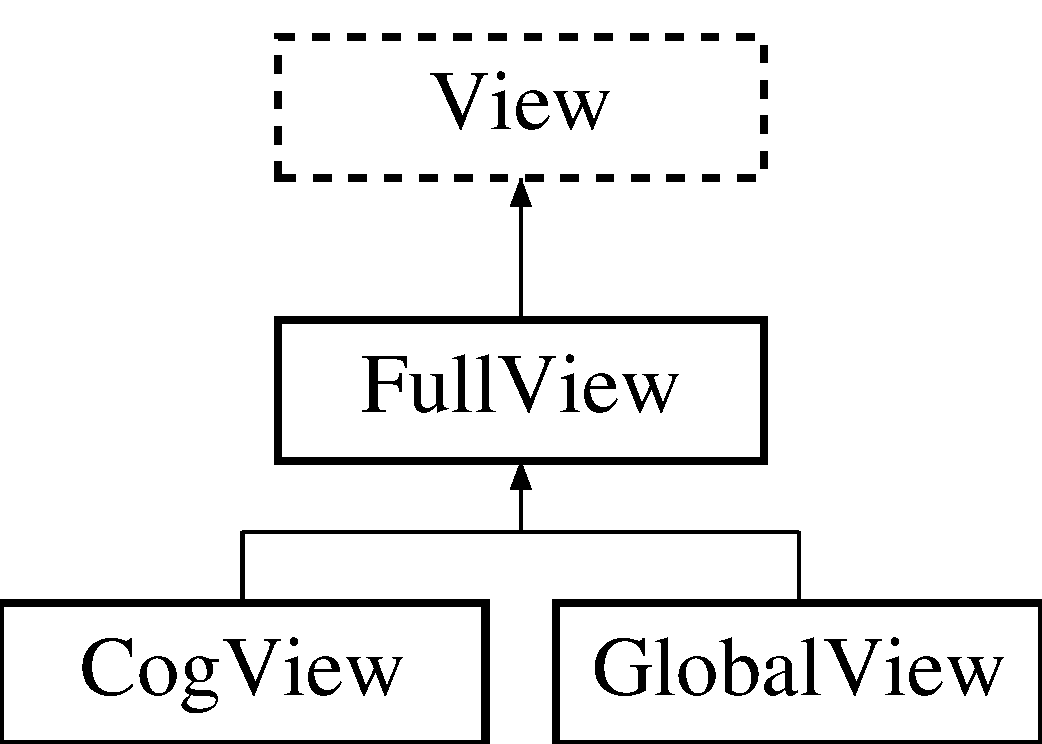
\includegraphics[height=3cm]{class_full_view}
\end{center}
\end{figure}
\subsection*{Protected Member Functions}
\begin{CompactItemize}
\item 
\hypertarget{class_full_view_2cf3b852e0fe260e10720d0d15c7f955}{
virtual std::set$<$ RobotRef $>$ \textbf{get\_\-visible\_\-robots} (const \hyperlink{class_robot_data}{RobotData} \&robot) const }
\label{class_full_view_2cf3b852e0fe260e10720d0d15c7f955}

\item 
\hypertarget{class_full_view_c70e733b24bcff73a2396738c2b0b7d5}{
virtual std::set$<$ ObstacleRef $>$ \textbf{get\_\-visible\_\-obstacles} (const \hyperlink{class_robot_data}{RobotData} \&robot) const }
\label{class_full_view_c70e733b24bcff73a2396738c2b0b7d5}

\item 
\hypertarget{class_full_view_cd69a9cdcc846e1b3f6394f0221b395c}{
virtual std::set$<$ MarkerRef $>$ \textbf{get\_\-visible\_\-markers} (const \hyperlink{class_robot_data}{RobotData} \&robot) const }
\label{class_full_view_cd69a9cdcc846e1b3f6394f0221b395c}

\end{CompactItemize}


\subsection{Detailed Description}
All objects visible to all robots view model. 

Provides implementations of getVisible... methods.

Assigning this class to a Robot corresponds to a \char`\"{}all objects visible to all robots\char`\"{} model. 

Definition at line 22 of file full\_\-view.h.

The documentation for this class was generated from the following files:\begin{CompactItemize}
\item 
src/Views/full\_\-view.h\item 
src/Views/full\_\-view.cc\end{CompactItemize}

\hypertarget{class_global_view}{
\section{GlobalView Class Reference}
\label{class_global_view}\index{GlobalView@{GlobalView}}
}
Global information view model.  


{\tt \#include $<$global\_\-view.h$>$}

Inheritance diagram for GlobalView::\begin{figure}[H]
\begin{center}
\leavevmode
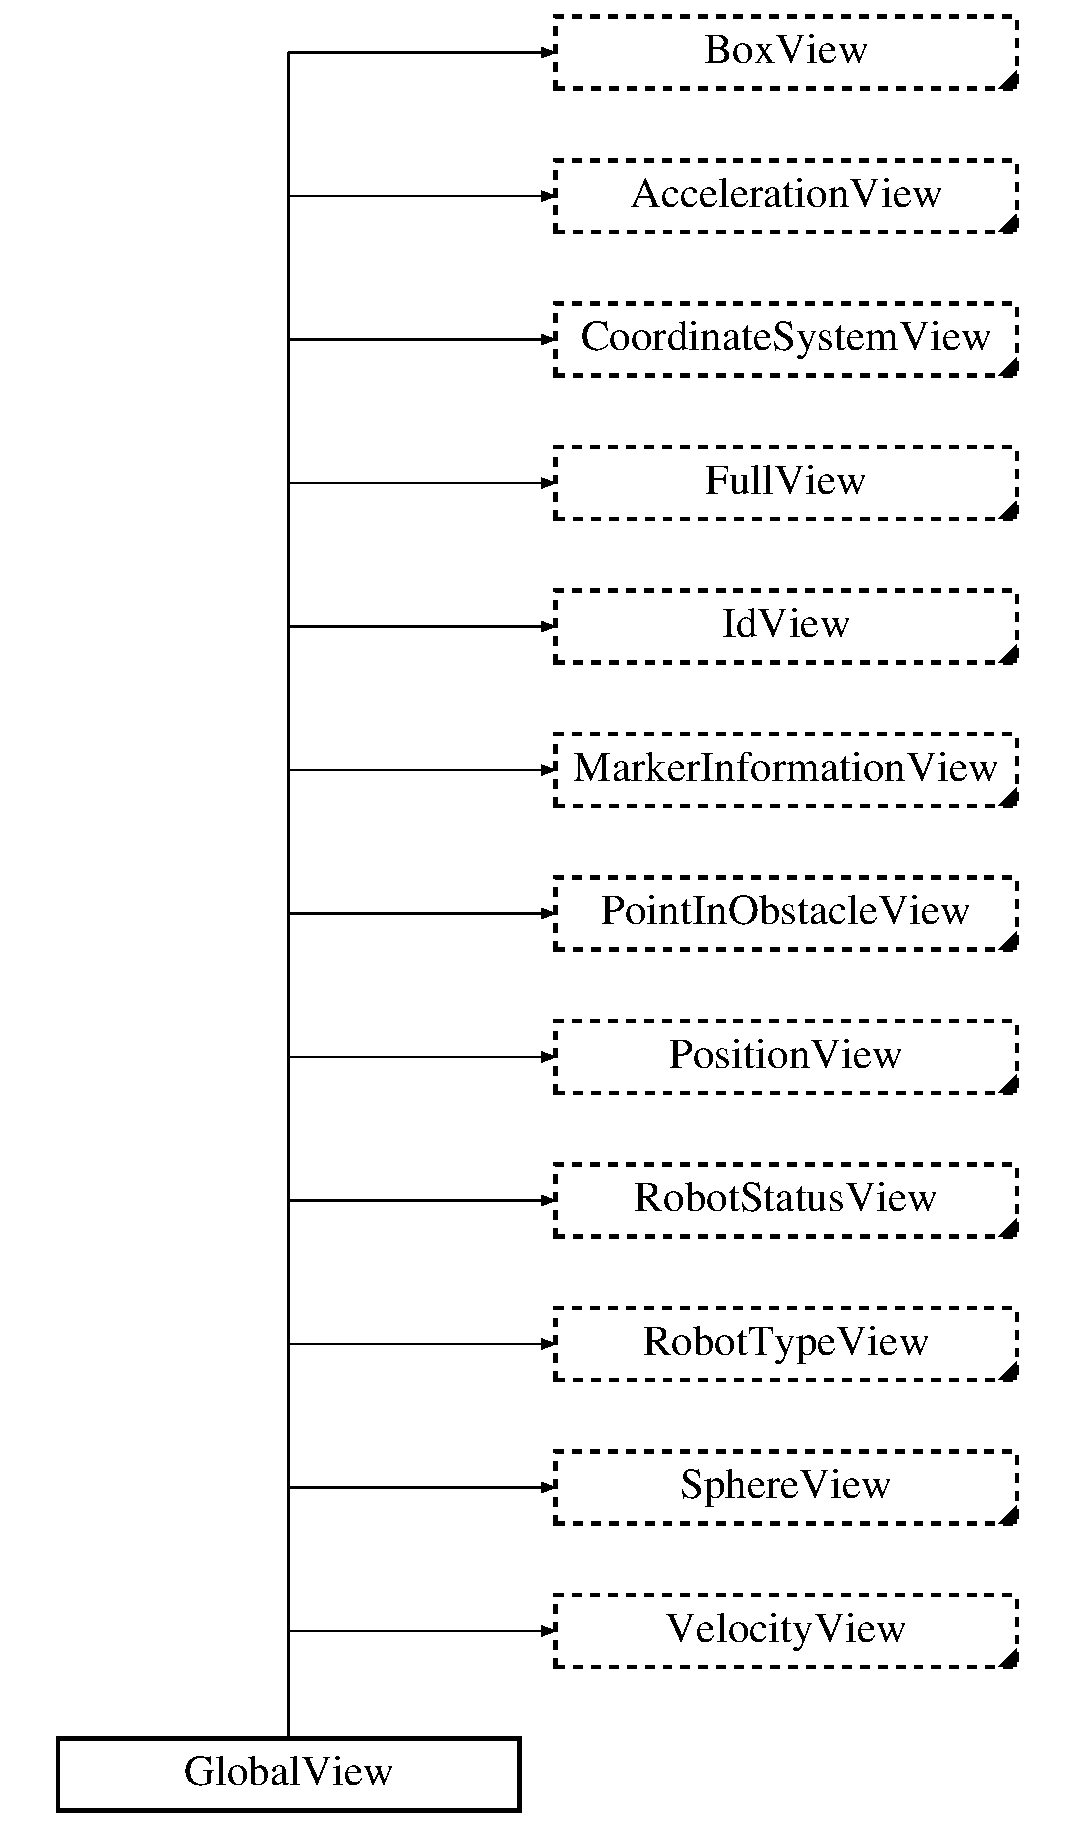
\includegraphics[height=12cm]{class_global_view}
\end{center}
\end{figure}


\subsection{Detailed Description}
Global information view model. 

Assigning this class to a Robot corresponds to a \char`\"{}see everything, everywhere\char`\"{} model. 

Definition at line 32 of file global\_\-view.h.

The documentation for this class was generated from the following files:\begin{CompactItemize}
\item 
src/Views/global\_\-view.h\item 
src/Views/global\_\-view.cc\end{CompactItemize}

\hypertarget{class_handle_requests_event}{
\section{HandleRequestsEvent Class Reference}
\label{class_handle_requests_event}\index{HandleRequestsEvent@{HandleRequestsEvent}}
}
A \hyperlink{class_handle_requests_event}{HandleRequestsEvent} is an event which causes a set of requests to be handled by the event handler.  


{\tt \#include $<$handle\_\-requests\_\-event.h$>$}

Inheritance diagram for HandleRequestsEvent::\begin{figure}[H]
\begin{center}
\leavevmode
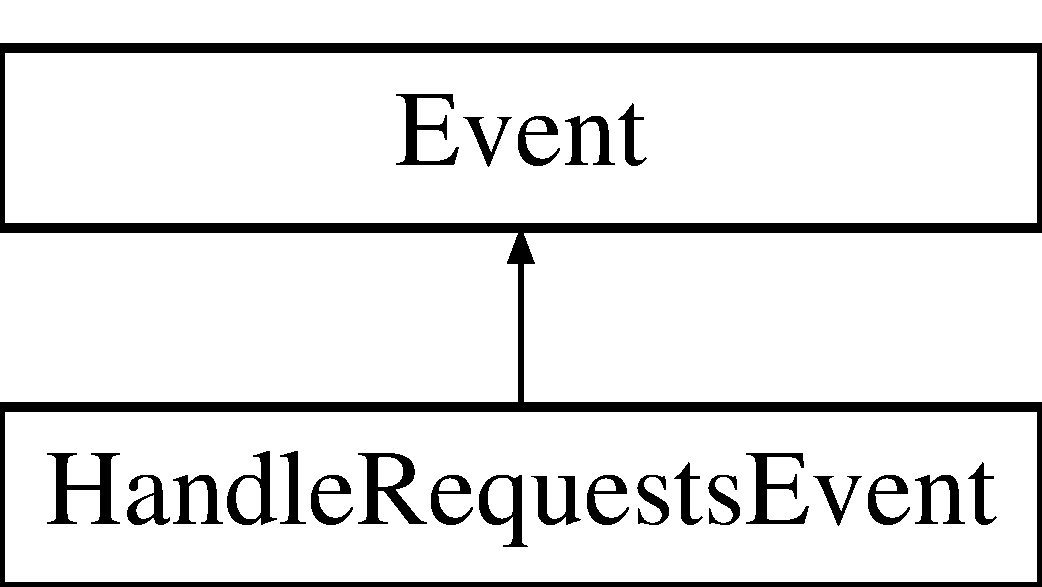
\includegraphics[height=2cm]{class_handle_requests_event}
\end{center}
\end{figure}
\subsection*{Public Member Functions}
\begin{CompactItemize}
\item 
\hypertarget{class_handle_requests_event_02097b7eb6a26773b12fcc6ec7be7335}{
\textbf{HandleRequestsEvent} (int time)}
\label{class_handle_requests_event_02097b7eb6a26773b12fcc6ec7be7335}

\item 
void \hyperlink{class_handle_requests_event_9d8db560c776cba3f19050f8a0b58ce3}{add\_\-to\_\-requests} (boost::shared\_\-ptr$<$ const \hyperlink{class_request}{Request} $>$ new\_\-request)
\item 
const vector$<$ boost::shared\_\-ptr$<$ const \hyperlink{class_request}{Request} $>$ $>$ \& \hyperlink{class_handle_requests_event_a03318f80549212e2023cdab01c9f924}{requests} () const 
\end{CompactItemize}
\subsection*{Private Attributes}
\begin{CompactItemize}
\item 
vector$<$ boost::shared\_\-ptr$<$ const \hyperlink{class_request}{Request} $>$ $>$ \hyperlink{class_handle_requests_event_38fd31bb391f81b55c1ec15de8a4bd00}{requests\_\-}
\end{CompactItemize}


\subsection{Detailed Description}
A \hyperlink{class_handle_requests_event}{HandleRequestsEvent} is an event which causes a set of requests to be handled by the event handler. 

Definition at line 24 of file handle\_\-requests\_\-event.h.

\subsection{Member Function Documentation}
\hypertarget{class_handle_requests_event_9d8db560c776cba3f19050f8a0b58ce3}{
\index{HandleRequestsEvent@{HandleRequestsEvent}!add\_\-to\_\-requests@{add\_\-to\_\-requests}}
\index{add\_\-to\_\-requests@{add\_\-to\_\-requests}!HandleRequestsEvent@{HandleRequestsEvent}}
\subsubsection[add\_\-to\_\-requests]{\setlength{\rightskip}{0pt plus 5cm}void HandleRequestsEvent::add\_\-to\_\-requests (boost::shared\_\-ptr$<$ const {\bf Request} $>$ {\em new\_\-request})}}
\label{class_handle_requests_event_9d8db560c776cba3f19050f8a0b58ce3}


Adds a new request to the set of requests. \begin{Desc}
\item[Parameters:]
\begin{description}
\item[{\em A}]shared pointer to the new request. \end{description}
\end{Desc}


Definition at line 10 of file handle\_\-requests\_\-event.cc.

References requests\_\-.

Referenced by SynchronousASG::get\_\-next\_\-event().\hypertarget{class_handle_requests_event_a03318f80549212e2023cdab01c9f924}{
\index{HandleRequestsEvent@{HandleRequestsEvent}!requests@{requests}}
\index{requests@{requests}!HandleRequestsEvent@{HandleRequestsEvent}}
\subsubsection[requests]{\setlength{\rightskip}{0pt plus 5cm}const vector$<$ boost::shared\_\-ptr$<$ const {\bf Request} $>$ $>$ \& HandleRequestsEvent::requests () const}}
\label{class_handle_requests_event_a03318f80549212e2023cdab01c9f924}


Returns a constant reference to the set of requests. \begin{Desc}
\item[Returns:]A constant reference to the set of requests. \end{Desc}


Definition at line 14 of file handle\_\-requests\_\-event.cc.

References requests\_\-.

\subsection{Member Data Documentation}
\hypertarget{class_handle_requests_event_38fd31bb391f81b55c1ec15de8a4bd00}{
\index{HandleRequestsEvent@{HandleRequestsEvent}!requests\_\-@{requests\_\-}}
\index{requests\_\-@{requests\_\-}!HandleRequestsEvent@{HandleRequestsEvent}}
\subsubsection[requests\_\-]{\setlength{\rightskip}{0pt plus 5cm}vector$<$boost::shared\_\-ptr$<$const {\bf Request}$>$ $>$ {\bf HandleRequestsEvent::requests\_\-}\hspace{0.3cm}{\tt  \mbox{[}private\mbox{]}}}}
\label{class_handle_requests_event_38fd31bb391f81b55c1ec15de8a4bd00}


The set of resulting requests 

Definition at line 45 of file handle\_\-requests\_\-event.h.

Referenced by add\_\-to\_\-requests(), and requests().

The documentation for this class was generated from the following files:\begin{CompactItemize}
\item 
src/Events/handle\_\-requests\_\-event.h\item 
src/Events/handle\_\-requests\_\-event.cc\end{CompactItemize}

\hypertarget{class_history}{
\section{History Class Reference}
\label{class_history}\index{History@{History}}
}
\hyperlink{class_history}{History} of the simulation The history class maintains a circular buffer to store past simulation states. It provides thread safe accessor to the buffer.  


{\tt \#include $<$history.h$>$}

\subsection*{Public Member Functions}
\begin{CompactItemize}
\item 
\hyperlink{class_history_29c644a10ab5e5f533b7e0dad3282550}{History} (std::size\_\-t size)
\item 
void \hyperlink{class_history_552af5c8e63ab3f8470d5143a8f91cdf}{insert} (boost::shared\_\-ptr$<$ \hyperlink{class_world_information}{WorldInformation} $>$ world\_\-information)
\item 
boost::shared\_\-ptr$<$ \hyperlink{class_world_information}{WorldInformation} $>$ \hyperlink{class_history_db58449276c5cd1da3837c233e908382}{get\_\-oldest\_\-unused} (bool block=false)
\item 
const \hyperlink{class_world_information}{WorldInformation} \& \hyperlink{class_history_bca19bfe4b9a2a4dea9c2ac42a22b4ab}{get\_\-newest} () const 
\end{CompactItemize}
\subsection*{Private Attributes}
\begin{CompactItemize}
\item 
\hypertarget{class_history_650374a2e1175423c867a77bd0d31075}{
boost::circular\_\-buffer$<$ boost::shared\_\-ptr$<$ \hyperlink{class_world_information}{WorldInformation} $>$ $>$ \textbf{history\_\-}}
\label{class_history_650374a2e1175423c867a77bd0d31075}

\item 
\hypertarget{class_history_323b31291bbed2a143bc4ba2c6607a4c}{
std::size\_\-t \textbf{consumer\_\-position\_\-}}
\label{class_history_323b31291bbed2a143bc4ba2c6607a4c}

\item 
\hypertarget{class_history_14eb7399599a276b8943137e0173e1bc}{
boost::interprocess::interprocess\_\-semaphore \textbf{empty\_\-count\_\-}}
\label{class_history_14eb7399599a276b8943137e0173e1bc}

\item 
\hypertarget{class_history_128179c2c8bd17ccbf429bda72b08d8d}{
boost::interprocess::interprocess\_\-semaphore \textbf{fill\_\-count\_\-}}
\label{class_history_128179c2c8bd17ccbf429bda72b08d8d}

\item 
\hypertarget{class_history_8030f931d185354ebf5576789625e404}{
boost::mutex \textbf{mutex\_\-}}
\label{class_history_8030f931d185354ebf5576789625e404}

\end{CompactItemize}


\subsection{Detailed Description}
\hyperlink{class_history}{History} of the simulation The history class maintains a circular buffer to store past simulation states. It provides thread safe accessor to the buffer. 

Definition at line 24 of file history.h.

\subsection{Constructor \& Destructor Documentation}
\hypertarget{class_history_29c644a10ab5e5f533b7e0dad3282550}{
\index{History@{History}!History@{History}}
\index{History@{History}!History@{History}}
\subsubsection[History]{\setlength{\rightskip}{0pt plus 5cm}History::History (std::size\_\-t {\em size})}}
\label{class_history_29c644a10ab5e5f533b7e0dad3282550}


creates a new history with given size 

Definition at line 14 of file history.cc.

\subsection{Member Function Documentation}
\hypertarget{class_history_552af5c8e63ab3f8470d5143a8f91cdf}{
\index{History@{History}!insert@{insert}}
\index{insert@{insert}!History@{History}}
\subsubsection[insert]{\setlength{\rightskip}{0pt plus 5cm}void History::insert (boost::shared\_\-ptr$<$ {\bf WorldInformation} $>$ {\em world\_\-information})}}
\label{class_history_552af5c8e63ab3f8470d5143a8f91cdf}


inserts a new \hyperlink{class_world_information}{WorldInformation} object into the history 

Definition at line 18 of file history.cc.\hypertarget{class_history_db58449276c5cd1da3837c233e908382}{
\index{History@{History}!get\_\-oldest\_\-unused@{get\_\-oldest\_\-unused}}
\index{get\_\-oldest\_\-unused@{get\_\-oldest\_\-unused}!History@{History}}
\subsubsection[get\_\-oldest\_\-unused]{\setlength{\rightskip}{0pt plus 5cm}boost::shared\_\-ptr$<$ {\bf WorldInformation} $>$ History::get\_\-oldest\_\-unused (bool {\em block} = {\tt false})}}
\label{class_history_db58449276c5cd1da3837c233e908382}


gets the oldest \hyperlink{class_world_information}{WorldInformation} object in the buffer as copy and marks it as consumed. If no consumeable \hyperlink{class_world_information}{WorldInformation} is available either the thread is blocked (blocked = true) or a NULL pointer is returned (block = false). 

Definition at line 30 of file history.cc.\hypertarget{class_history_bca19bfe4b9a2a4dea9c2ac42a22b4ab}{
\index{History@{History}!get\_\-newest@{get\_\-newest}}
\index{get\_\-newest@{get\_\-newest}!History@{History}}
\subsubsection[get\_\-newest]{\setlength{\rightskip}{0pt plus 5cm}const {\bf WorldInformation} \& History::get\_\-newest () const}}
\label{class_history_bca19bfe4b9a2a4dea9c2ac42a22b4ab}


returns a const reference to the newest world information object in the buffer. Should never be called if there is another thread which might call push\_\-back() concurrently 

Definition at line 47 of file history.cc.

The documentation for this class was generated from the following files:\begin{CompactItemize}
\item 
src/SimulationControl/history.h\item 
src/SimulationControl/history.cc\end{CompactItemize}

\hypertarget{class_identifier}{
\section{Identifier Class Reference}
\label{class_identifier}\index{Identifier@{Identifier}}
}
Denote ID's of robots.  


{\tt \#include $<$identifier.h$>$}

Inheritance diagram for Identifier::\begin{figure}[H]
\begin{center}
\leavevmode
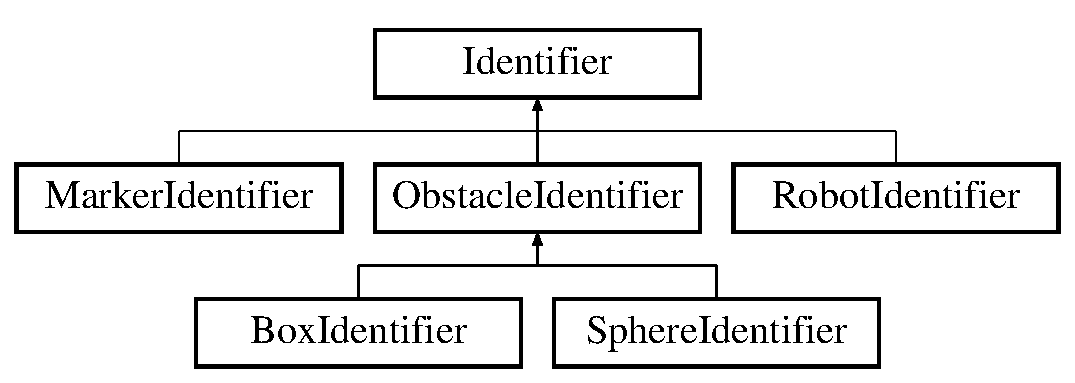
\includegraphics[height=3cm]{class_identifier}
\end{center}
\end{figure}
\subsection*{Public Member Functions}
\begin{CompactItemize}
\item 
\hypertarget{class_identifier_1f3dc42a16ac34879e694cca9cda3c00}{
virtual boost::shared\_\-ptr$<$ \hyperlink{class_identifier}{Identifier} $>$ \textbf{clone} () const =0}
\label{class_identifier_1f3dc42a16ac34879e694cca9cda3c00}

\end{CompactItemize}
\subsection*{Protected Member Functions}
\begin{CompactItemize}
\item 
\hypertarget{class_identifier_d5b9459c4949aa660a8823cc99e25bf1}{
\textbf{Identifier} (std::size\_\-t id)}
\label{class_identifier_d5b9459c4949aa660a8823cc99e25bf1}

\item 
std::size\_\-t \hyperlink{class_identifier_b60899833fdfebb88f78ecf4c71a2f78}{id} () const 
\end{CompactItemize}
\subsection*{Private Attributes}
\begin{CompactItemize}
\item 
\hypertarget{class_identifier_fb77402eef7f10eeb2a3f4251390a007}{
std::size\_\-t \textbf{id\_\-}}
\label{class_identifier_fb77402eef7f10eeb2a3f4251390a007}

\end{CompactItemize}
\subsection*{Friends}
\begin{CompactItemize}
\item 
\hypertarget{class_identifier_018ff8a950133459fda57a235706a80b}{
class \hyperlink{class_identifier_018ff8a950133459fda57a235706a80b}{View}}
\label{class_identifier_018ff8a950133459fda57a235706a80b}

\item 
\hypertarget{class_identifier_d26290837413ac85ad8f757b518bbe77}{
class \hyperlink{class_identifier_d26290837413ac85ad8f757b518bbe77}{WorldInformation}}
\label{class_identifier_d26290837413ac85ad8f757b518bbe77}

\item 
\hypertarget{class_identifier_b80291af9c262f63b83fa9c16f12014d}{
class \textbf{Parser}}
\label{class_identifier_b80291af9c262f63b83fa9c16f12014d}

\item 
\hypertarget{class_identifier_1c533f013e578e25f6831e9076855ec8}{
class \textbf{write\_\-obstacle\_\-1}}
\label{class_identifier_1c533f013e578e25f6831e9076855ec8}

\end{CompactItemize}
\subsection*{Classes}
\begin{CompactItemize}
\item 
class \textbf{Comp}
\end{CompactItemize}


\subsection{Detailed Description}
Denote ID's of robots. 

\begin{Desc}
\item[Author:]Martina Hüllmann \end{Desc}


Definition at line 13 of file identifier.h.

\subsection{Member Function Documentation}
\hypertarget{class_identifier_b60899833fdfebb88f78ecf4c71a2f78}{
\index{Identifier@{Identifier}!id@{id}}
\index{id@{id}!Identifier@{Identifier}}
\subsubsection[id]{\setlength{\rightskip}{0pt plus 5cm}std::size\_\-t Identifier::id () const\hspace{0.3cm}{\tt  \mbox{[}protected\mbox{]}}}}
\label{class_identifier_b60899833fdfebb88f78ecf4c71a2f78}


Return ID of identifier. \begin{Desc}
\item[Returns:]ID of identifier. \end{Desc}


Definition at line 12 of file identifier.cc.

The documentation for this class was generated from the following files:\begin{CompactItemize}
\item 
src/Model/identifier.h\item 
src/Model/identifier.cc\end{CompactItemize}

\hypertarget{class_look_event}{
\section{LookEvent Class Reference}
\label{class_look_event}\index{LookEvent@{LookEvent}}
}
A \hyperlink{class_look_event}{LookEvent} is an event which causes a subset of the robots to recieve new information about the world.  


{\tt \#include $<$look\_\-event.h$>$}

Inheritance diagram for LookEvent::\begin{figure}[H]
\begin{center}
\leavevmode
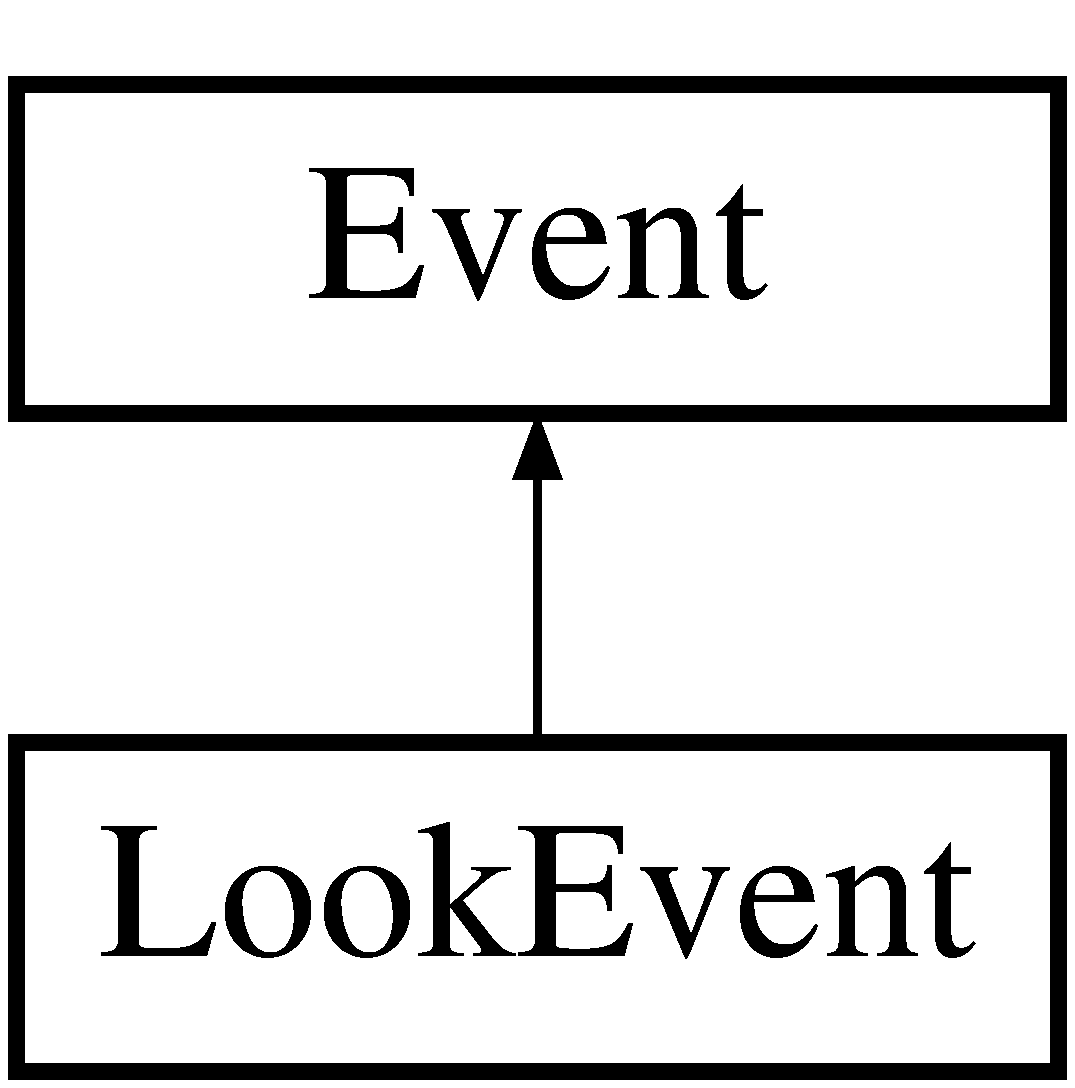
\includegraphics[height=2cm]{class_look_event}
\end{center}
\end{figure}
\subsection*{Public Member Functions}
\begin{CompactItemize}
\item 
\hypertarget{class_look_event_d1f3c66e1562c94f0e63564ec10ec599}{
\textbf{LookEvent} (int time)}
\label{class_look_event_d1f3c66e1562c94f0e63564ec10ec599}

\item 
void \hyperlink{class_look_event_69ea06b306f36339e6e5fbe3ffa7b1b8}{add\_\-to\_\-robot\_\-subset} (boost::shared\_\-ptr$<$ Robot $>$ new\_\-robot)
\item 
const vector$<$ boost::shared\_\-ptr$<$ Robot $>$ $>$ \& \hyperlink{class_look_event_3c33e32768298a315a0a242c823ea957}{robot\_\-subset} () const 
\end{CompactItemize}
\subsection*{Private Attributes}
\begin{CompactItemize}
\item 
vector$<$ boost::shared\_\-ptr$<$ Robot $>$ $>$ \hyperlink{class_look_event_a01e6d88edc4ae67bd1db1632eafb55f}{robot\_\-subset\_\-}
\end{CompactItemize}


\subsection{Detailed Description}
A \hyperlink{class_look_event}{LookEvent} is an event which causes a subset of the robots to recieve new information about the world. 

Definition at line 24 of file look\_\-event.h.

\subsection{Member Function Documentation}
\hypertarget{class_look_event_69ea06b306f36339e6e5fbe3ffa7b1b8}{
\index{LookEvent@{LookEvent}!add\_\-to\_\-robot\_\-subset@{add\_\-to\_\-robot\_\-subset}}
\index{add\_\-to\_\-robot\_\-subset@{add\_\-to\_\-robot\_\-subset}!LookEvent@{LookEvent}}
\subsubsection[add\_\-to\_\-robot\_\-subset]{\setlength{\rightskip}{0pt plus 5cm}void LookEvent::add\_\-to\_\-robot\_\-subset (boost::shared\_\-ptr$<$ Robot $>$ {\em new\_\-robot})}}
\label{class_look_event_69ea06b306f36339e6e5fbe3ffa7b1b8}


Adds a new robot to the subset of robots in the event. \begin{Desc}
\item[Parameters:]
\begin{description}
\item[{\em a}]shared pointer to the new robot \end{description}
\end{Desc}


Definition at line 10 of file look\_\-event.cc.

References robot\_\-subset\_\-.

Referenced by SynchronousASG::get\_\-next\_\-event().\hypertarget{class_look_event_3c33e32768298a315a0a242c823ea957}{
\index{LookEvent@{LookEvent}!robot\_\-subset@{robot\_\-subset}}
\index{robot\_\-subset@{robot\_\-subset}!LookEvent@{LookEvent}}
\subsubsection[robot\_\-subset]{\setlength{\rightskip}{0pt plus 5cm}const vector$<$ boost::shared\_\-ptr$<$ Robot $>$ $>$ \& LookEvent::robot\_\-subset () const}}
\label{class_look_event_3c33e32768298a315a0a242c823ea957}


Returns a constant reference to the robot subset. \begin{Desc}
\item[Returns:]A constant reference to the robot subset. \end{Desc}


Definition at line 15 of file look\_\-event.cc.

References robot\_\-subset\_\-.

\subsection{Member Data Documentation}
\hypertarget{class_look_event_a01e6d88edc4ae67bd1db1632eafb55f}{
\index{LookEvent@{LookEvent}!robot\_\-subset\_\-@{robot\_\-subset\_\-}}
\index{robot\_\-subset\_\-@{robot\_\-subset\_\-}!LookEvent@{LookEvent}}
\subsubsection[robot\_\-subset\_\-]{\setlength{\rightskip}{0pt plus 5cm}vector$<$boost::shared\_\-ptr$<$Robot$>$ $>$ {\bf LookEvent::robot\_\-subset\_\-}\hspace{0.3cm}{\tt  \mbox{[}private\mbox{]}}}}
\label{class_look_event_a01e6d88edc4ae67bd1db1632eafb55f}


The robot subset for this event. 

Definition at line 45 of file look\_\-event.h.

Referenced by add\_\-to\_\-robot\_\-subset(), and robot\_\-subset().

The documentation for this class was generated from the following files:\begin{CompactItemize}
\item 
src/Events/look\_\-event.h\item 
src/Events/look\_\-event.cc\end{CompactItemize}

\hypertarget{class_marker_identifier}{
\section{MarkerIdentifier Class Reference}
\label{class_marker_identifier}\index{MarkerIdentifier@{MarkerIdentifier}}
}
Denote ID's of markers.  


{\tt \#include $<$marker\_\-identifier.h$>$}

Inheritance diagram for MarkerIdentifier::\begin{figure}[H]
\begin{center}
\leavevmode
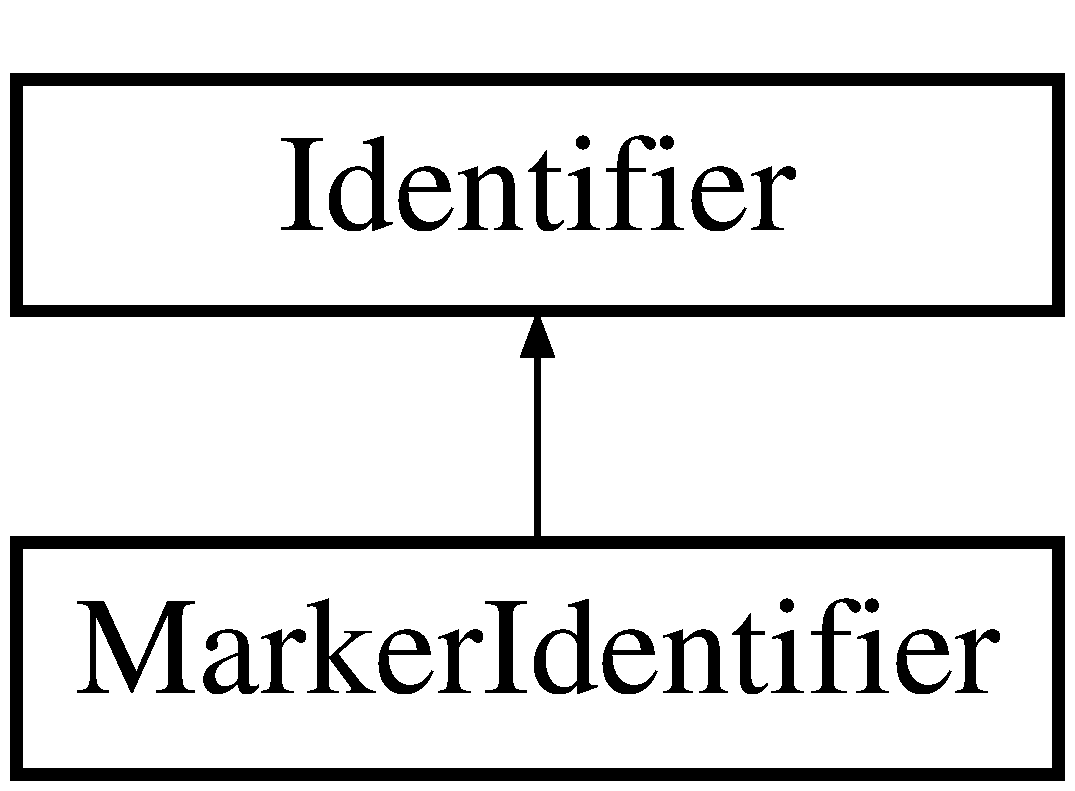
\includegraphics[height=2cm]{class_marker_identifier}
\end{center}
\end{figure}
\subsection*{Public Member Functions}
\begin{CompactItemize}
\item 
\hypertarget{class_marker_identifier_2b872bb640d730f586898bfec6bdccd9}{
virtual boost::shared\_\-ptr$<$ \hyperlink{class_identifier}{Identifier} $>$ \textbf{clone} () const }
\label{class_marker_identifier_2b872bb640d730f586898bfec6bdccd9}

\end{CompactItemize}
\subsection*{Protected Member Functions}
\begin{CompactItemize}
\item 
\hypertarget{class_marker_identifier_25454cbe8affbdec98269f46a59a40a7}{
\textbf{MarkerIdentifier} (size\_\-t id)}
\label{class_marker_identifier_25454cbe8affbdec98269f46a59a40a7}

\end{CompactItemize}
\subsection*{Friends}
\begin{CompactItemize}
\item 
\hypertarget{class_marker_identifier_6433c824d5e64fc5b3635b2a0f2af16c}{
class \textbf{SimpleWorldFixture}}
\label{class_marker_identifier_6433c824d5e64fc5b3635b2a0f2af16c}

\end{CompactItemize}


\subsection{Detailed Description}
Denote ID's of markers. 

\begin{Desc}
\item[Author:]Martina Hüllmann \end{Desc}


Definition at line 12 of file marker\_\-identifier.h.

The documentation for this class was generated from the following files:\begin{CompactItemize}
\item 
src/Model/marker\_\-identifier.h\item 
src/Model/marker\_\-identifier.cc\end{CompactItemize}

\hypertarget{class_marker_information}{
\section{MarkerInformation Class Reference}
\label{class_marker_information}\index{MarkerInformation@{MarkerInformation}}
}
TODO insert description here.  


{\tt \#include $<$marker\_\-information.h$>$}

\subsection*{Public Member Functions}
\begin{CompactItemize}
\item 
virtual boost::shared\_\-ptr$<$ \hyperlink{class_marker_information}{MarkerInformation} $>$ \hyperlink{class_marker_information_8ca33ead76cd7206804ee5dc38176b31}{clone} () const 
\end{CompactItemize}


\subsection{Detailed Description}
TODO insert description here. 

Definition at line 15 of file marker\_\-information.h.

\subsection{Member Function Documentation}
\hypertarget{class_marker_information_8ca33ead76cd7206804ee5dc38176b31}{
\index{MarkerInformation@{MarkerInformation}!clone@{clone}}
\index{clone@{clone}!MarkerInformation@{MarkerInformation}}
\subsubsection[clone]{\setlength{\rightskip}{0pt plus 5cm}boost::shared\_\-ptr$<$ {\bf MarkerInformation} $>$ MarkerInformation::clone () const\hspace{0.3cm}{\tt  \mbox{[}virtual\mbox{]}}}}
\label{class_marker_information_8ca33ead76cd7206804ee5dc38176b31}


Clones this object and returns a shared ptr to the cloned object. typeid($\ast$this) == typeid($\ast$clone) \begin{Desc}
\item[Returns:]shared ptr to the cloned object \end{Desc}


Definition at line 12 of file marker\_\-information.cc.

The documentation for this class was generated from the following files:\begin{CompactItemize}
\item 
src/Model/marker\_\-information.h\item 
src/Model/marker\_\-information.cc\end{CompactItemize}

\hypertarget{class_marker_request}{
\section{MarkerRequest Class Reference}
\label{class_marker_request}\index{MarkerRequest@{MarkerRequest}}
}
A Marker \hyperlink{class_request}{Request} is issued by a robot which wants to change its marker information.  


{\tt \#include $<$marker\_\-request.h$>$}

Inheritance diagram for MarkerRequest::\begin{figure}[H]
\begin{center}
\leavevmode
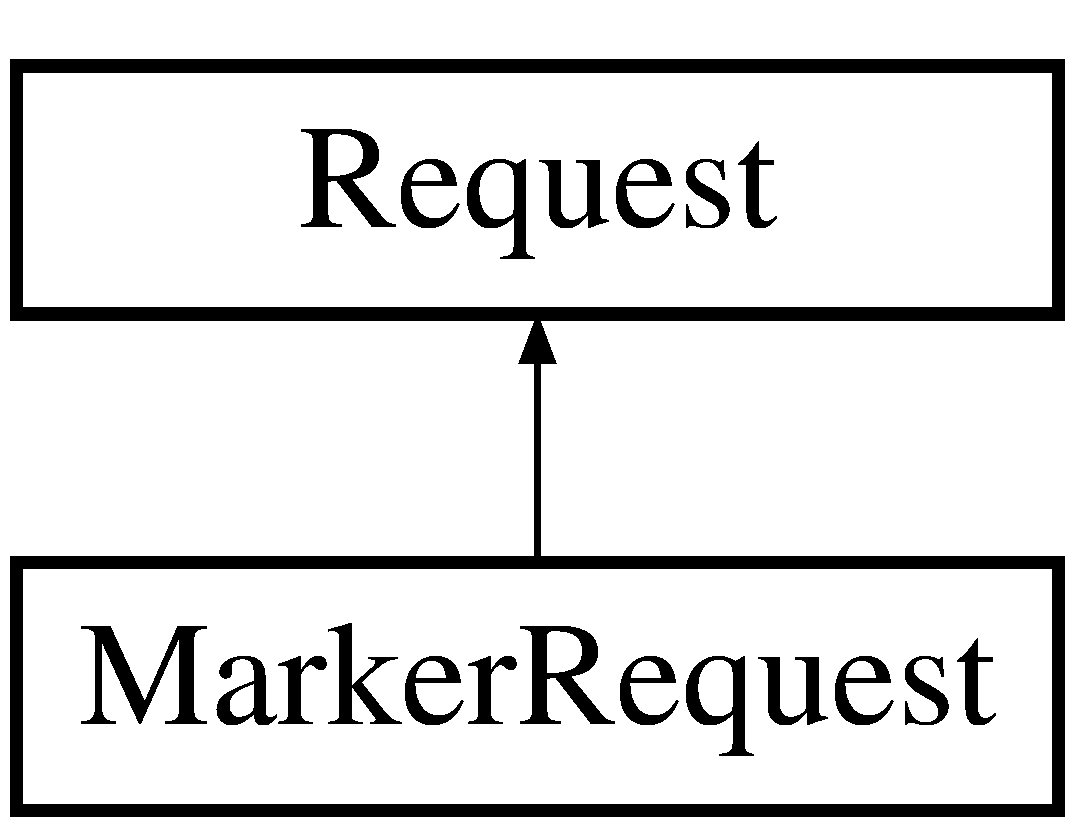
\includegraphics[height=2cm]{class_marker_request}
\end{center}
\end{figure}
\subsection*{Public Member Functions}
\begin{CompactItemize}
\item 
\hyperlink{class_marker_request_70e6f1fa26f348ec9cfc8e9880a4bb29}{MarkerRequest} (Robot \&robot, boost::shared\_\-ptr$<$ \hyperlink{class_marker_information}{MarkerInformation} $>$ requested\_\-marker\_\-information)
\item 
const \hyperlink{class_marker_information}{MarkerInformation} \& \hyperlink{class_marker_request_709617b7716a3f5305782bc18067d357}{requested\_\-marker\_\-information} () const 
\end{CompactItemize}
\subsection*{Private Attributes}
\begin{CompactItemize}
\item 
\hypertarget{class_marker_request_663c5ca8defcffb014b12787068ff94d}{
boost::shared\_\-ptr$<$ \hyperlink{class_marker_information}{MarkerInformation} $>$ \textbf{requested\_\-marker\_\-information\_\-}}
\label{class_marker_request_663c5ca8defcffb014b12787068ff94d}

\end{CompactItemize}


\subsection{Detailed Description}
A Marker \hyperlink{class_request}{Request} is issued by a robot which wants to change its marker information. 

Notes: The request cannot be changed after creating. 

Definition at line 21 of file marker\_\-request.h.

\subsection{Constructor \& Destructor Documentation}
\hypertarget{class_marker_request_70e6f1fa26f348ec9cfc8e9880a4bb29}{
\index{MarkerRequest@{MarkerRequest}!MarkerRequest@{MarkerRequest}}
\index{MarkerRequest@{MarkerRequest}!MarkerRequest@{MarkerRequest}}
\subsubsection[MarkerRequest]{\setlength{\rightskip}{0pt plus 5cm}MarkerRequest::MarkerRequest (Robot \& {\em robot}, \/  boost::shared\_\-ptr$<$ {\bf MarkerInformation} $>$ {\em requested\_\-marker\_\-information})\hspace{0.3cm}{\tt  \mbox{[}inline\mbox{]}}}}
\label{class_marker_request_70e6f1fa26f348ec9cfc8e9880a4bb29}


constructs a new \hyperlink{class_marker_request}{MarkerRequest}. The request cannot be changed after constructing. 

Definition at line 27 of file marker\_\-request.h.

\subsection{Member Function Documentation}
\hypertarget{class_marker_request_709617b7716a3f5305782bc18067d357}{
\index{MarkerRequest@{MarkerRequest}!requested\_\-marker\_\-information@{requested\_\-marker\_\-information}}
\index{requested\_\-marker\_\-information@{requested\_\-marker\_\-information}!MarkerRequest@{MarkerRequest}}
\subsubsection[requested\_\-marker\_\-information]{\setlength{\rightskip}{0pt plus 5cm}const {\bf MarkerInformation}\& MarkerRequest::requested\_\-marker\_\-information () const\hspace{0.3cm}{\tt  \mbox{[}inline\mbox{]}}}}
\label{class_marker_request_709617b7716a3f5305782bc18067d357}


Returns a constant reference to the requested marker information  A constant reference to the requested marker information 

Definition at line 35 of file marker\_\-request.h.

The documentation for this class was generated from the following file:\begin{CompactItemize}
\item 
src/Requests/marker\_\-request.h\end{CompactItemize}

\hypertarget{class_marker_request_handler}{
\section{MarkerRequestHandler Class Reference}
\label{class_marker_request_handler}\index{MarkerRequestHandler@{MarkerRequestHandler}}
}
{\tt \#include $<$marker\_\-request\_\-handler.h$>$}

Inheritance diagram for MarkerRequestHandler::\begin{figure}[H]
\begin{center}
\leavevmode
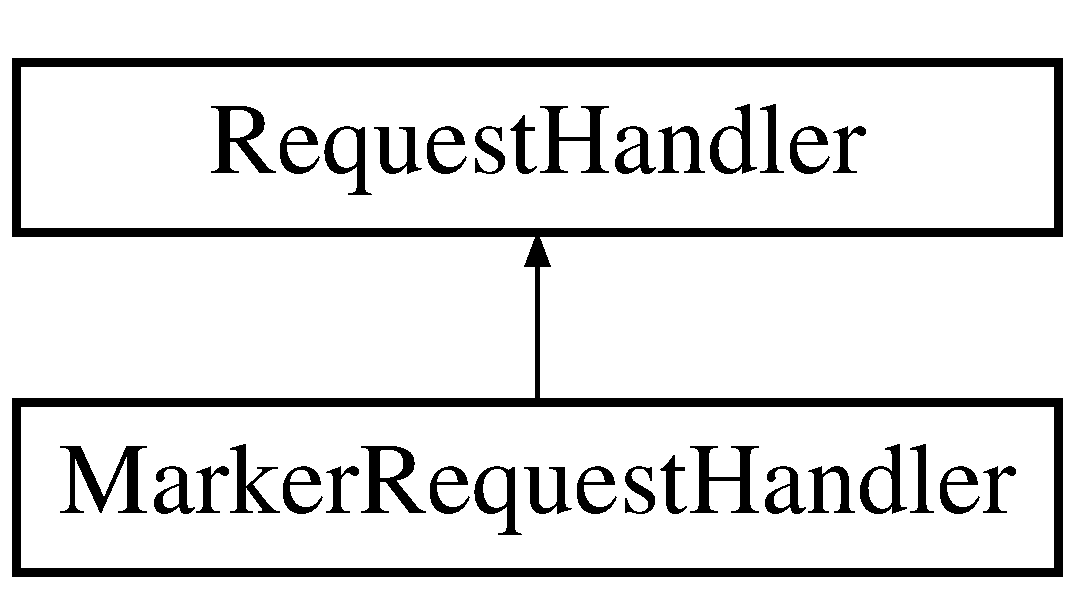
\includegraphics[height=2cm]{class_marker_request_handler}
\end{center}
\end{figure}
\subsection*{Public Member Functions}
\begin{CompactItemize}
\item 
\hypertarget{class_marker_request_handler_5e1961178d8824f7f209107e4f4c49c9}{
\textbf{MarkerRequestHandler} (unsigned int seed, double discard\_\-probability, const \hyperlink{class_history}{History} \&history)}
\label{class_marker_request_handler_5e1961178d8824f7f209107e4f4c49c9}

\end{CompactItemize}
\subsection*{Private Member Functions}
\begin{CompactItemize}
\item 
\hypertarget{class_marker_request_handler_653344108cddbff3f2163a64821ba730}{
virtual void \textbf{handle\_\-request\_\-reliable} (boost::shared\_\-ptr$<$ \hyperlink{class_world_information}{WorldInformation} $>$ world\_\-information, boost::shared\_\-ptr$<$ const \hyperlink{class_request}{Request} $>$ request)}
\label{class_marker_request_handler_653344108cddbff3f2163a64821ba730}

\end{CompactItemize}


\subsection{Detailed Description}
Standard marker request handler. Fullfills every marker request. 

Definition at line 16 of file marker\_\-request\_\-handler.h.

The documentation for this class was generated from the following files:\begin{CompactItemize}
\item 
src/EventHandlers/marker\_\-request\_\-handler.h\item 
src/EventHandlers/marker\_\-request\_\-handler.cc\end{CompactItemize}

\hypertarget{class_neighbor_view}{
\section{NeighborView Class Reference}
\label{class_neighbor_view}\index{NeighborView@{NeighborView}}
}
Basic k-nearest-neighbor view model.  


{\tt \#include $<$neighbor\_\-view.h$>$}

Inheritance diagram for NeighborView::\begin{figure}[H]
\begin{center}
\leavevmode
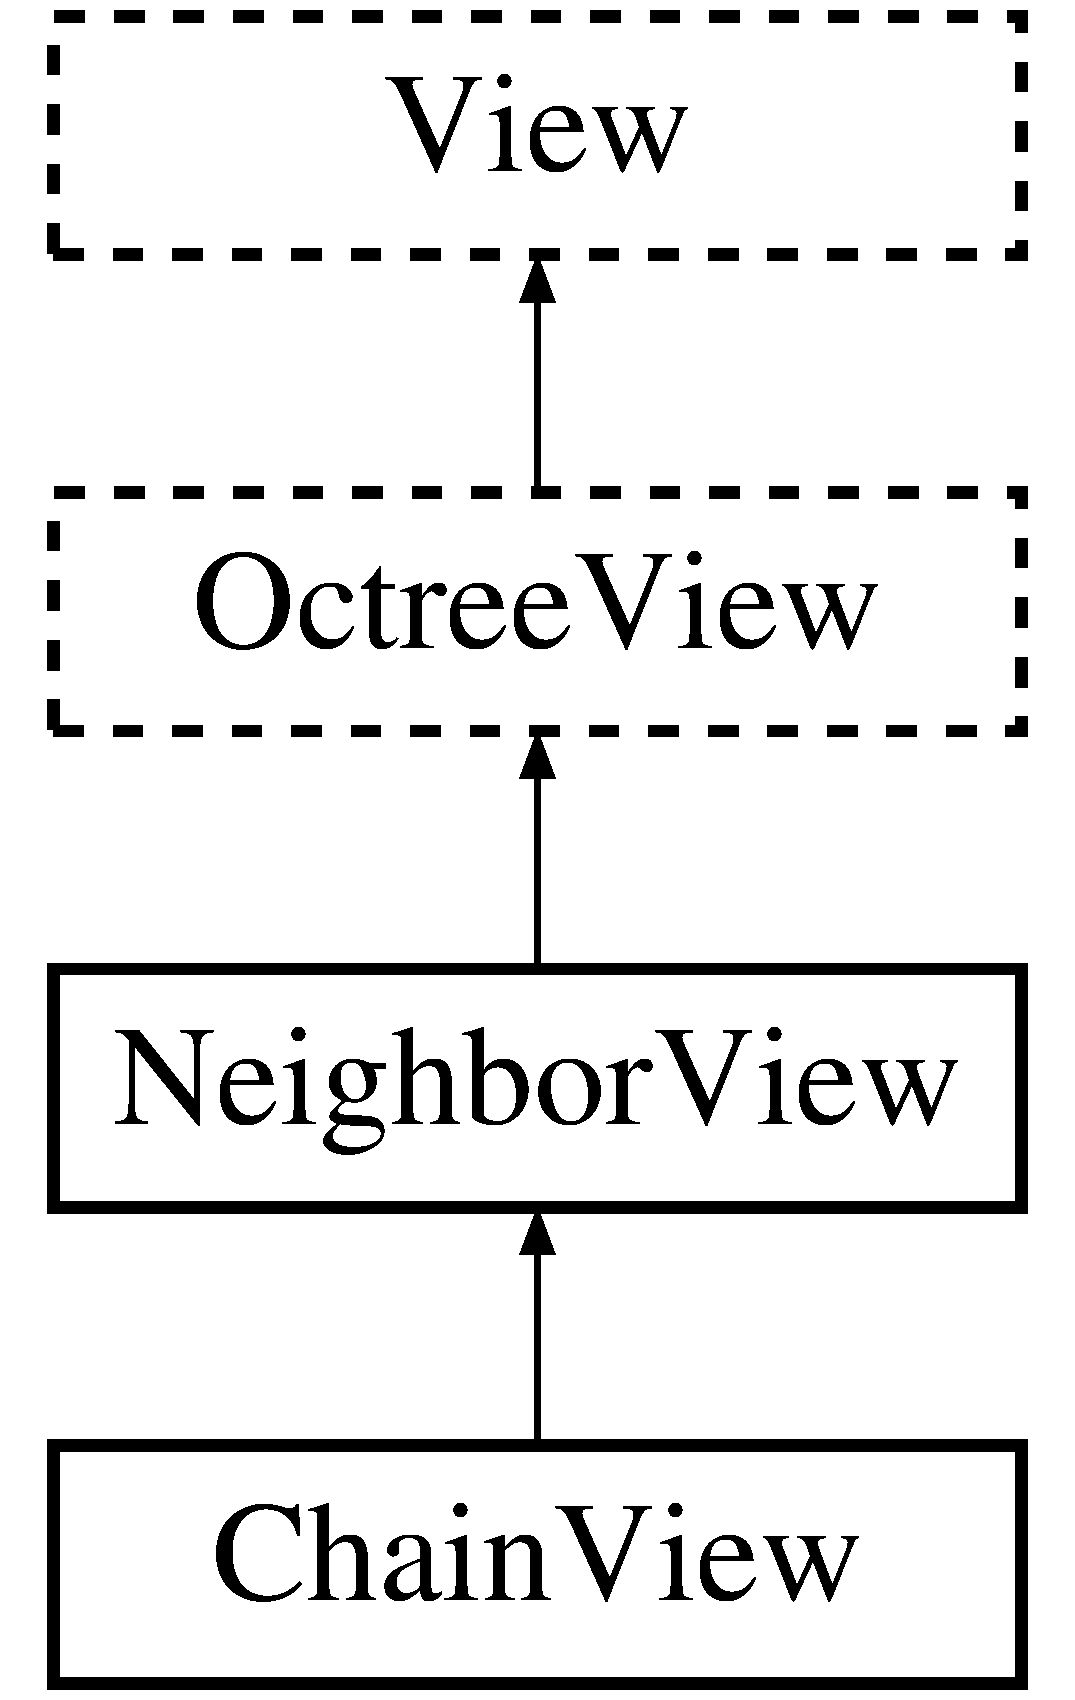
\includegraphics[height=4cm]{class_neighbor_view}
\end{center}
\end{figure}
\subsection*{Public Member Functions}
\begin{CompactItemize}
\item 
\hypertarget{class_neighbor_view_ca4206dd5c6a4c50499c1cf95ef6fb7e}{
\textbf{NeighborView} (unsigned seen\_\-objects\_\-count)}
\label{class_neighbor_view_ca4206dd5c6a4c50499c1cf95ef6fb7e}

\end{CompactItemize}
\subsection*{Protected Member Functions}
\begin{CompactItemize}
\item 
\hypertarget{class_neighbor_view_f443b8f5e8dd1d6becc02d694fee24a8}{
virtual std::set$<$ RobotRef $>$ \textbf{get\_\-visible\_\-robots} (const \hyperlink{class_robot_data}{RobotData} \&robot) const }
\label{class_neighbor_view_f443b8f5e8dd1d6becc02d694fee24a8}

\item 
\hypertarget{class_neighbor_view_2ecce04a8e257db985ad626ed4a0188f}{
virtual std::set$<$ ObstacleRef $>$ \textbf{get\_\-visible\_\-obstacles} (const \hyperlink{class_robot_data}{RobotData} \&robot) const }
\label{class_neighbor_view_2ecce04a8e257db985ad626ed4a0188f}

\item 
\hypertarget{class_neighbor_view_32e118b43fcecba1bf78276f70717a5e}{
virtual std::set$<$ MarkerRef $>$ \textbf{get\_\-visible\_\-markers} (const \hyperlink{class_robot_data}{RobotData} \&robot) const }
\label{class_neighbor_view_32e118b43fcecba1bf78276f70717a5e}

\item 
\hypertarget{class_neighbor_view_1cbcfcdebfa7e573ef73536a0c8fec2c}{
unsigned \textbf{seen\_\-objects\_\-count} () const }
\label{class_neighbor_view_1cbcfcdebfa7e573ef73536a0c8fec2c}

\end{CompactItemize}
\subsection*{Private Attributes}
\begin{CompactItemize}
\item 
\hypertarget{class_neighbor_view_d5a3d924c1a46f2ebcbb06c17bdfbf9b}{
unsigned \textbf{seen\_\-objects\_\-count\_\-}}
\label{class_neighbor_view_d5a3d924c1a46f2ebcbb06c17bdfbf9b}

\end{CompactItemize}


\subsection{Detailed Description}
Basic k-nearest-neighbor view model. 

Provides implementations of getVisible... methods. To efficiently implement them the classes uses an \hyperlink{class_octree}{Octree} as internal data structure.

Assigning this class to a Robot corresponds to a \char`\"{}see the k nearest objects\char`\"{} model. 

Definition at line 23 of file neighbor\_\-view.h.

The documentation for this class was generated from the following files:\begin{CompactItemize}
\item 
src/Views/neighbor\_\-view.h\item 
src/Views/neighbor\_\-view.cc\end{CompactItemize}

\hypertarget{class_num_set_stats}{
\section{NumSetStats Class Reference}
\label{class_num_set_stats}\index{NumSetStats@{NumSetStats}}
}
creates information on a numerical set  


{\tt \#include $<$numset\_\-stats.h$>$}

\subsection*{Public Member Functions}
\begin{CompactItemize}
\item 
\hyperlink{class_num_set_stats_889c116c12f1f1d08b71c78393abc2e4}{NumSetStats} ()
\item 
\hyperlink{class_num_set_stats_6453c26039df38b6a9dd8e5c039d1db1}{NumSetStats} (int cfg)
\item 
const int \hyperlink{class_num_set_stats_93c7b65ee1d6b2b618cf6d4fff0909ee}{cfg} () const 
\item 
void \hyperlink{class_num_set_stats_6306db6c6b350053c548421871ff9599}{set\_\-cfg} (int cfg)
\item 
void \hyperlink{class_num_set_stats_097be7d38f92b8618f9c5f5e8e86d07b}{handle} (const std::vector$<$ double $>$ \&data)
\item 
const double \hyperlink{class_num_set_stats_a20ab577f51080f3798a825a6392fda2}{min} () const 
\item 
const double \hyperlink{class_num_set_stats_ca1e3149eda7dc53aa884b577f61a12f}{max} () const 
\item 
const double \hyperlink{class_num_set_stats_36ddcdd2cdc3c01ae0b5253e26f3599e}{diam} () const 
\item 
const double \hyperlink{class_num_set_stats_c89ea68555e034fc8ad61a24e8105bbc}{avg} () const 
\item 
const double \hyperlink{class_num_set_stats_8576d0ce14fa99580e6f78666c841637}{sum} () const 
\item 
const double \hyperlink{class_num_set_stats_09c585c3187b3355b9c4e4f20bdef394}{abssum} () const 
\item 
const double \hyperlink{class_num_set_stats_09e5689d2b6635e1f7bf42cfb38d511c}{median} () const 
\item 
const double \hyperlink{class_num_set_stats_e531b9144515a839e21b0a9c9c74daae}{stddeviation} () const 
\item 
const std::string \hyperlink{class_num_set_stats_639732de39c31d82ade97d8e204db3c0}{to\_\-string} () const 
\end{CompactItemize}
\subsection*{Static Public Attributes}
\begin{CompactItemize}
\item 
static const int \hyperlink{class_num_set_stats_a650f090e33b5d6e21b4cb20d567d7d4}{MIN} = 0x01
\item 
static const int \hyperlink{class_num_set_stats_b9a7841be40024bbf113e9c936b3deab}{MAX} = 0x02
\item 
static const int \hyperlink{class_num_set_stats_b1820301209131d98f7cfab065d0440f}{DIAM} = 0x04
\item 
static const int \hyperlink{class_num_set_stats_c862317b59207332f5e0c8542ca31ce6}{AVG} = 0x08
\item 
static const int \hyperlink{class_num_set_stats_cc13e2095d277cf2e864e0fcb9504014}{MEDIAN} = 0x10
\item 
static const int \hyperlink{class_num_set_stats_d6d1e1e12eb76587059af855219f02a3}{SUM} = 0x20
\item 
static const int \hyperlink{class_num_set_stats_afd3e476b938988fc3ed9aef347d83f8}{ABSSUM} = 0x40
\item 
static const int \hyperlink{class_num_set_stats_e7880d38dc58838bda30a0554ef7af59}{STDDEVIATION} = 0x80
\item 
static const int \hyperlink{class_num_set_stats_0d368de57b461369635aced38be32b25}{DEFAULT} = \hyperlink{class_num_set_stats_a650f090e33b5d6e21b4cb20d567d7d4}{MIN}$|$\hyperlink{class_num_set_stats_b9a7841be40024bbf113e9c936b3deab}{MAX}$|$\hyperlink{class_num_set_stats_b1820301209131d98f7cfab065d0440f}{DIAM}$|$\hyperlink{class_num_set_stats_c862317b59207332f5e0c8542ca31ce6}{AVG}$|$\hyperlink{class_num_set_stats_e7880d38dc58838bda30a0554ef7af59}{STDDEVIATION}
\item 
static const int \hyperlink{class_num_set_stats_4e4f9d0b733c13f3c6feb99cde24bcec}{ALL} = 0xFFFFFFFF
\end{CompactItemize}
\subsection*{Private Member Functions}
\begin{CompactItemize}
\item 
void \hyperlink{class_num_set_stats_c16a5891e33db010aac26d062de620fd}{init} ()
\end{CompactItemize}
\subsection*{Private Attributes}
\begin{CompactItemize}
\item 
int \hyperlink{class_num_set_stats_a70473f5a35e86e19224550b7a919871}{cfg\_\-}
\item 
double \hyperlink{class_num_set_stats_e268eba5a003e3932b16e90ce8bad405}{min\_\-}
\item 
\hypertarget{class_num_set_stats_f5f15a621edab3e612c2d7430c78f892}{
double \textbf{max\_\-}}
\label{class_num_set_stats_f5f15a621edab3e612c2d7430c78f892}

\item 
\hypertarget{class_num_set_stats_87b5909c45d4fbe93fc16ab142e93bf6}{
double \textbf{diam\_\-}}
\label{class_num_set_stats_87b5909c45d4fbe93fc16ab142e93bf6}

\item 
\hypertarget{class_num_set_stats_1f384a596365ae07382cc5301493fe4a}{
double \textbf{avg\_\-}}
\label{class_num_set_stats_1f384a596365ae07382cc5301493fe4a}

\item 
\hypertarget{class_num_set_stats_def1065f51479ef02a8f4dbdc0f28c2c}{
double \textbf{median\_\-}}
\label{class_num_set_stats_def1065f51479ef02a8f4dbdc0f28c2c}

\item 
\hypertarget{class_num_set_stats_50d3d004ede70cd212499d5568f1fdc6}{
double \textbf{sum\_\-}}
\label{class_num_set_stats_50d3d004ede70cd212499d5568f1fdc6}

\item 
\hypertarget{class_num_set_stats_9a1f6e0f9634df90757a34da7ba9e7d7}{
double \textbf{abssum\_\-}}
\label{class_num_set_stats_9a1f6e0f9634df90757a34da7ba9e7d7}

\item 
\hypertarget{class_num_set_stats_a4ae52c9e1debca8595801eddb27e202}{
double \textbf{stddeviation\_\-}}
\label{class_num_set_stats_a4ae52c9e1debca8595801eddb27e202}

\end{CompactItemize}


\subsection{Detailed Description}
creates information on a numerical set 

\begin{Desc}
\item[Author:]Sven Kurras 1. create an instance of this class 2. configure it by a $|$$|$-combination of the various bitflags that are given as static ints in the class. Pass the configuration to the constructor or to set\_\-cfg(...)-function. 3. call handle(...) on a vector of the numbers to analyse. The currently configured information will now become (re)calculated. 4. read out the information by the respective getter-function or get an overview of all configured information by the \hyperlink{class_num_set_stats_639732de39c31d82ade97d8e204db3c0}{to\_\-string()}-function. 5. continue with any of the points above. \end{Desc}


Definition at line 23 of file numset\_\-stats.h.

\subsection{Constructor \& Destructor Documentation}
\hypertarget{class_num_set_stats_889c116c12f1f1d08b71c78393abc2e4}{
\index{NumSetStats@{NumSetStats}!NumSetStats@{NumSetStats}}
\index{NumSetStats@{NumSetStats}!NumSetStats@{NumSetStats}}
\subsubsection[NumSetStats]{\setlength{\rightskip}{0pt plus 5cm}NumSetStats::NumSetStats ()\hspace{0.3cm}{\tt  \mbox{[}explicit\mbox{]}}}}
\label{class_num_set_stats_889c116c12f1f1d08b71c78393abc2e4}


default constructor 

Definition at line 9 of file numset\_\-stats.cc.

References cfg\_\-, and DEFAULT.\hypertarget{class_num_set_stats_6453c26039df38b6a9dd8e5c039d1db1}{
\index{NumSetStats@{NumSetStats}!NumSetStats@{NumSetStats}}
\index{NumSetStats@{NumSetStats}!NumSetStats@{NumSetStats}}
\subsubsection[NumSetStats]{\setlength{\rightskip}{0pt plus 5cm}NumSetStats::NumSetStats (int {\em cfg})\hspace{0.3cm}{\tt  \mbox{[}explicit\mbox{]}}}}
\label{class_num_set_stats_6453c26039df38b6a9dd8e5c039d1db1}


constructor with initial configuration \begin{Desc}
\item[Parameters:]
\begin{description}
\item[{\em the}]cfg-flag-combination to use \end{description}
\end{Desc}


Definition at line 13 of file numset\_\-stats.cc.

References cfg\_\-.

\subsection{Member Function Documentation}
\hypertarget{class_num_set_stats_93c7b65ee1d6b2b618cf6d4fff0909ee}{
\index{NumSetStats@{NumSetStats}!cfg@{cfg}}
\index{cfg@{cfg}!NumSetStats@{NumSetStats}}
\subsubsection[cfg]{\setlength{\rightskip}{0pt plus 5cm}const int NumSetStats::cfg () const}}
\label{class_num_set_stats_93c7b65ee1d6b2b618cf6d4fff0909ee}


\begin{Desc}
\item[Returns:]current configuration-flags \end{Desc}


Definition at line 20 of file numset\_\-stats.cc.

References cfg\_\-.\hypertarget{class_num_set_stats_6306db6c6b350053c548421871ff9599}{
\index{NumSetStats@{NumSetStats}!set\_\-cfg@{set\_\-cfg}}
\index{set\_\-cfg@{set\_\-cfg}!NumSetStats@{NumSetStats}}
\subsubsection[set\_\-cfg]{\setlength{\rightskip}{0pt plus 5cm}void NumSetStats::set\_\-cfg (int {\em cfg})}}
\label{class_num_set_stats_6306db6c6b350053c548421871ff9599}


\begin{Desc}
\item[Parameters:]
\begin{description}
\item[{\em cfg}]new configuration-flags to use \end{description}
\end{Desc}


Definition at line 24 of file numset\_\-stats.cc.

References cfg\_\-.\hypertarget{class_num_set_stats_097be7d38f92b8618f9c5f5e8e86d07b}{
\index{NumSetStats@{NumSetStats}!handle@{handle}}
\index{handle@{handle}!NumSetStats@{NumSetStats}}
\subsubsection[handle]{\setlength{\rightskip}{0pt plus 5cm}void NumSetStats::handle (const std::vector$<$ double $>$ \& {\em data})}}
\label{class_num_set_stats_097be7d38f92b8618f9c5f5e8e86d07b}


Calculates all information on the numerical data in this vector that is requested by the currently set flags. Access the individual information via the respective getter-function, or all combined as a string via the \hyperlink{class_num_set_stats_639732de39c31d82ade97d8e204db3c0}{to\_\-string()}-function. \begin{Desc}
\item[Parameters:]
\begin{description}
\item[{\em data}]the numerical data to analyse \end{description}
\end{Desc}


Definition at line 37 of file numset\_\-stats.cc.

References cfg\_\-, init(), MEDIAN, and min\_\-.\hypertarget{class_num_set_stats_a20ab577f51080f3798a825a6392fda2}{
\index{NumSetStats@{NumSetStats}!min@{min}}
\index{min@{min}!NumSetStats@{NumSetStats}}
\subsubsection[min]{\setlength{\rightskip}{0pt plus 5cm}const double NumSetStats::min () const}}
\label{class_num_set_stats_a20ab577f51080f3798a825a6392fda2}


\begin{Desc}
\item[Returns:]latest calculated minimum-value, unspecified if not calculated \end{Desc}


Definition at line 77 of file numset\_\-stats.cc.

References min\_\-.\hypertarget{class_num_set_stats_ca1e3149eda7dc53aa884b577f61a12f}{
\index{NumSetStats@{NumSetStats}!max@{max}}
\index{max@{max}!NumSetStats@{NumSetStats}}
\subsubsection[max]{\setlength{\rightskip}{0pt plus 5cm}const double NumSetStats::max () const}}
\label{class_num_set_stats_ca1e3149eda7dc53aa884b577f61a12f}


\begin{Desc}
\item[Returns:]latest calculated maximum-value, unspecified if not calculated \end{Desc}


Definition at line 81 of file numset\_\-stats.cc.\hypertarget{class_num_set_stats_36ddcdd2cdc3c01ae0b5253e26f3599e}{
\index{NumSetStats@{NumSetStats}!diam@{diam}}
\index{diam@{diam}!NumSetStats@{NumSetStats}}
\subsubsection[diam]{\setlength{\rightskip}{0pt plus 5cm}const double NumSetStats::diam () const}}
\label{class_num_set_stats_36ddcdd2cdc3c01ae0b5253e26f3599e}


\begin{Desc}
\item[Returns:]latest calculated diameter-value (max-min) unspecified if not calculated \end{Desc}


Definition at line 85 of file numset\_\-stats.cc.\hypertarget{class_num_set_stats_c89ea68555e034fc8ad61a24e8105bbc}{
\index{NumSetStats@{NumSetStats}!avg@{avg}}
\index{avg@{avg}!NumSetStats@{NumSetStats}}
\subsubsection[avg]{\setlength{\rightskip}{0pt plus 5cm}const double NumSetStats::avg () const}}
\label{class_num_set_stats_c89ea68555e034fc8ad61a24e8105bbc}


\begin{Desc}
\item[Returns:]latest calculated average-value, unspecified if not calculated \end{Desc}


Definition at line 89 of file numset\_\-stats.cc.\hypertarget{class_num_set_stats_8576d0ce14fa99580e6f78666c841637}{
\index{NumSetStats@{NumSetStats}!sum@{sum}}
\index{sum@{sum}!NumSetStats@{NumSetStats}}
\subsubsection[sum]{\setlength{\rightskip}{0pt plus 5cm}const double NumSetStats::sum () const}}
\label{class_num_set_stats_8576d0ce14fa99580e6f78666c841637}


\begin{Desc}
\item[Returns:]latest calculated overall-sum, unspecified if not calculated \end{Desc}


Definition at line 93 of file numset\_\-stats.cc.\hypertarget{class_num_set_stats_09c585c3187b3355b9c4e4f20bdef394}{
\index{NumSetStats@{NumSetStats}!abssum@{abssum}}
\index{abssum@{abssum}!NumSetStats@{NumSetStats}}
\subsubsection[abssum]{\setlength{\rightskip}{0pt plus 5cm}const double NumSetStats::abssum () const}}
\label{class_num_set_stats_09c585c3187b3355b9c4e4f20bdef394}


\begin{Desc}
\item[Returns:]latest calculated overall-sum of absolute values, unspecified if not calculated \end{Desc}


Definition at line 97 of file numset\_\-stats.cc.\hypertarget{class_num_set_stats_09e5689d2b6635e1f7bf42cfb38d511c}{
\index{NumSetStats@{NumSetStats}!median@{median}}
\index{median@{median}!NumSetStats@{NumSetStats}}
\subsubsection[median]{\setlength{\rightskip}{0pt plus 5cm}const double NumSetStats::median () const}}
\label{class_num_set_stats_09e5689d2b6635e1f7bf42cfb38d511c}


\begin{Desc}
\item[Returns:]latest calculated median value, unspecified if not calculated \end{Desc}


Definition at line 101 of file numset\_\-stats.cc.\hypertarget{class_num_set_stats_e531b9144515a839e21b0a9c9c74daae}{
\index{NumSetStats@{NumSetStats}!stddeviation@{stddeviation}}
\index{stddeviation@{stddeviation}!NumSetStats@{NumSetStats}}
\subsubsection[stddeviation]{\setlength{\rightskip}{0pt plus 5cm}const double NumSetStats::stddeviation () const}}
\label{class_num_set_stats_e531b9144515a839e21b0a9c9c74daae}


\begin{Desc}
\item[Returns:]latest calculated standard-deviation, unspecified if not calculated \end{Desc}


Definition at line 105 of file numset\_\-stats.cc.\hypertarget{class_num_set_stats_639732de39c31d82ade97d8e204db3c0}{
\index{NumSetStats@{NumSetStats}!to\_\-string@{to\_\-string}}
\index{to\_\-string@{to\_\-string}!NumSetStats@{NumSetStats}}
\subsubsection[to\_\-string]{\setlength{\rightskip}{0pt plus 5cm}const std::string NumSetStats::to\_\-string () const}}
\label{class_num_set_stats_639732de39c31d82ade97d8e204db3c0}


\begin{Desc}
\item[Returns:]string-representation of all latest calculated values with flags set in cfg, unspecified if nothing calculated \end{Desc}


Definition at line 109 of file numset\_\-stats.cc.

References ABSSUM, AVG, cfg\_\-, DIAM, MAX, MEDIAN, MIN, min\_\-, STDDEVIATION, and SUM.\hypertarget{class_num_set_stats_c16a5891e33db010aac26d062de620fd}{
\index{NumSetStats@{NumSetStats}!init@{init}}
\index{init@{init}!NumSetStats@{NumSetStats}}
\subsubsection[init]{\setlength{\rightskip}{0pt plus 5cm}void NumSetStats::init ()\hspace{0.3cm}{\tt  \mbox{[}private\mbox{]}}}}
\label{class_num_set_stats_c16a5891e33db010aac26d062de620fd}


performs required initializations before calculation 

Definition at line 28 of file numset\_\-stats.cc.

References min\_\-.

Referenced by handle().

\subsection{Member Data Documentation}
\hypertarget{class_num_set_stats_a650f090e33b5d6e21b4cb20d567d7d4}{
\index{NumSetStats@{NumSetStats}!MIN@{MIN}}
\index{MIN@{MIN}!NumSetStats@{NumSetStats}}
\subsubsection[MIN]{\setlength{\rightskip}{0pt plus 5cm}const int {\bf NumSetStats::MIN} = 0x01\hspace{0.3cm}{\tt  \mbox{[}static\mbox{]}}}}
\label{class_num_set_stats_a650f090e33b5d6e21b4cb20d567d7d4}


flag for minimum 

Definition at line 30 of file numset\_\-stats.h.

Referenced by to\_\-string().\hypertarget{class_num_set_stats_b9a7841be40024bbf113e9c936b3deab}{
\index{NumSetStats@{NumSetStats}!MAX@{MAX}}
\index{MAX@{MAX}!NumSetStats@{NumSetStats}}
\subsubsection[MAX]{\setlength{\rightskip}{0pt plus 5cm}const int {\bf NumSetStats::MAX} = 0x02\hspace{0.3cm}{\tt  \mbox{[}static\mbox{]}}}}
\label{class_num_set_stats_b9a7841be40024bbf113e9c936b3deab}


flag for maximum 

Definition at line 35 of file numset\_\-stats.h.

Referenced by to\_\-string().\hypertarget{class_num_set_stats_b1820301209131d98f7cfab065d0440f}{
\index{NumSetStats@{NumSetStats}!DIAM@{DIAM}}
\index{DIAM@{DIAM}!NumSetStats@{NumSetStats}}
\subsubsection[DIAM]{\setlength{\rightskip}{0pt plus 5cm}const int {\bf NumSetStats::DIAM} = 0x04\hspace{0.3cm}{\tt  \mbox{[}static\mbox{]}}}}
\label{class_num_set_stats_b1820301209131d98f7cfab065d0440f}


flag for maximum 

Definition at line 40 of file numset\_\-stats.h.

Referenced by to\_\-string().\hypertarget{class_num_set_stats_c862317b59207332f5e0c8542ca31ce6}{
\index{NumSetStats@{NumSetStats}!AVG@{AVG}}
\index{AVG@{AVG}!NumSetStats@{NumSetStats}}
\subsubsection[AVG]{\setlength{\rightskip}{0pt plus 5cm}const int {\bf NumSetStats::AVG} = 0x08\hspace{0.3cm}{\tt  \mbox{[}static\mbox{]}}}}
\label{class_num_set_stats_c862317b59207332f5e0c8542ca31ce6}


flag for average 

Definition at line 45 of file numset\_\-stats.h.

Referenced by to\_\-string().\hypertarget{class_num_set_stats_cc13e2095d277cf2e864e0fcb9504014}{
\index{NumSetStats@{NumSetStats}!MEDIAN@{MEDIAN}}
\index{MEDIAN@{MEDIAN}!NumSetStats@{NumSetStats}}
\subsubsection[MEDIAN]{\setlength{\rightskip}{0pt plus 5cm}const int {\bf NumSetStats::MEDIAN} = 0x10\hspace{0.3cm}{\tt  \mbox{[}static\mbox{]}}}}
\label{class_num_set_stats_cc13e2095d277cf2e864e0fcb9504014}


flag for calculating median 

Definition at line 50 of file numset\_\-stats.h.

Referenced by handle(), and to\_\-string().\hypertarget{class_num_set_stats_d6d1e1e12eb76587059af855219f02a3}{
\index{NumSetStats@{NumSetStats}!SUM@{SUM}}
\index{SUM@{SUM}!NumSetStats@{NumSetStats}}
\subsubsection[SUM]{\setlength{\rightskip}{0pt plus 5cm}const int {\bf NumSetStats::SUM} = 0x20\hspace{0.3cm}{\tt  \mbox{[}static\mbox{]}}}}
\label{class_num_set_stats_d6d1e1e12eb76587059af855219f02a3}


flag for calculating the sum 

Definition at line 55 of file numset\_\-stats.h.

Referenced by to\_\-string().\hypertarget{class_num_set_stats_afd3e476b938988fc3ed9aef347d83f8}{
\index{NumSetStats@{NumSetStats}!ABSSUM@{ABSSUM}}
\index{ABSSUM@{ABSSUM}!NumSetStats@{NumSetStats}}
\subsubsection[ABSSUM]{\setlength{\rightskip}{0pt plus 5cm}const int {\bf NumSetStats::ABSSUM} = 0x40\hspace{0.3cm}{\tt  \mbox{[}static\mbox{]}}}}
\label{class_num_set_stats_afd3e476b938988fc3ed9aef347d83f8}


flag for calculating the sum of absolute values 

Definition at line 60 of file numset\_\-stats.h.

Referenced by to\_\-string().\hypertarget{class_num_set_stats_e7880d38dc58838bda30a0554ef7af59}{
\index{NumSetStats@{NumSetStats}!STDDEVIATION@{STDDEVIATION}}
\index{STDDEVIATION@{STDDEVIATION}!NumSetStats@{NumSetStats}}
\subsubsection[STDDEVIATION]{\setlength{\rightskip}{0pt plus 5cm}const int {\bf NumSetStats::STDDEVIATION} = 0x80\hspace{0.3cm}{\tt  \mbox{[}static\mbox{]}}}}
\label{class_num_set_stats_e7880d38dc58838bda30a0554ef7af59}


flag for calculating the standard deviation 

Definition at line 65 of file numset\_\-stats.h.

Referenced by to\_\-string().\hypertarget{class_num_set_stats_0d368de57b461369635aced38be32b25}{
\index{NumSetStats@{NumSetStats}!DEFAULT@{DEFAULT}}
\index{DEFAULT@{DEFAULT}!NumSetStats@{NumSetStats}}
\subsubsection[DEFAULT]{\setlength{\rightskip}{0pt plus 5cm}const int {\bf NumSetStats::DEFAULT} = {\bf MIN}$|${\bf MAX}$|${\bf DIAM}$|${\bf AVG}$|${\bf STDDEVIATION}\hspace{0.3cm}{\tt  \mbox{[}static\mbox{]}}}}
\label{class_num_set_stats_0d368de57b461369635aced38be32b25}


combined flag of default parameters 

Definition at line 70 of file numset\_\-stats.h.

Referenced by NumSetStats().\hypertarget{class_num_set_stats_4e4f9d0b733c13f3c6feb99cde24bcec}{
\index{NumSetStats@{NumSetStats}!ALL@{ALL}}
\index{ALL@{ALL}!NumSetStats@{NumSetStats}}
\subsubsection[ALL]{\setlength{\rightskip}{0pt plus 5cm}const int {\bf NumSetStats::ALL} = 0xFFFFFFFF\hspace{0.3cm}{\tt  \mbox{[}static\mbox{]}}}}
\label{class_num_set_stats_4e4f9d0b733c13f3c6feb99cde24bcec}


combined flag of all parameters 

Definition at line 75 of file numset\_\-stats.h.\hypertarget{class_num_set_stats_a70473f5a35e86e19224550b7a919871}{
\index{NumSetStats@{NumSetStats}!cfg\_\-@{cfg\_\-}}
\index{cfg\_\-@{cfg\_\-}!NumSetStats@{NumSetStats}}
\subsubsection[cfg\_\-]{\setlength{\rightskip}{0pt plus 5cm}int {\bf NumSetStats::cfg\_\-}\hspace{0.3cm}{\tt  \mbox{[}private\mbox{]}}}}
\label{class_num_set_stats_a70473f5a35e86e19224550b7a919871}


the current configuration of the calculation 

Definition at line 168 of file numset\_\-stats.h.

Referenced by cfg(), handle(), NumSetStats(), set\_\-cfg(), and to\_\-string().\hypertarget{class_num_set_stats_e268eba5a003e3932b16e90ce8bad405}{
\index{NumSetStats@{NumSetStats}!min\_\-@{min\_\-}}
\index{min\_\-@{min\_\-}!NumSetStats@{NumSetStats}}
\subsubsection[min\_\-]{\setlength{\rightskip}{0pt plus 5cm}double {\bf NumSetStats::min\_\-}\hspace{0.3cm}{\tt  \mbox{[}private\mbox{]}}}}
\label{class_num_set_stats_e268eba5a003e3932b16e90ce8bad405}


the values to calculate 

Definition at line 173 of file numset\_\-stats.h.

Referenced by handle(), init(), min(), and to\_\-string().

The documentation for this class was generated from the following files:\begin{CompactItemize}
\item 
src/Statistics/numset\_\-stats.h\item 
src/Statistics/numset\_\-stats.cc\end{CompactItemize}

\hypertarget{class_obstacle_identifier}{
\section{ObstacleIdentifier Class Reference}
\label{class_obstacle_identifier}\index{ObstacleIdentifier@{ObstacleIdentifier}}
}
Denote ID's of obstacles.  


{\tt \#include $<$obstacle\_\-identifier.h$>$}

Inheritance diagram for ObstacleIdentifier::\begin{figure}[H]
\begin{center}
\leavevmode
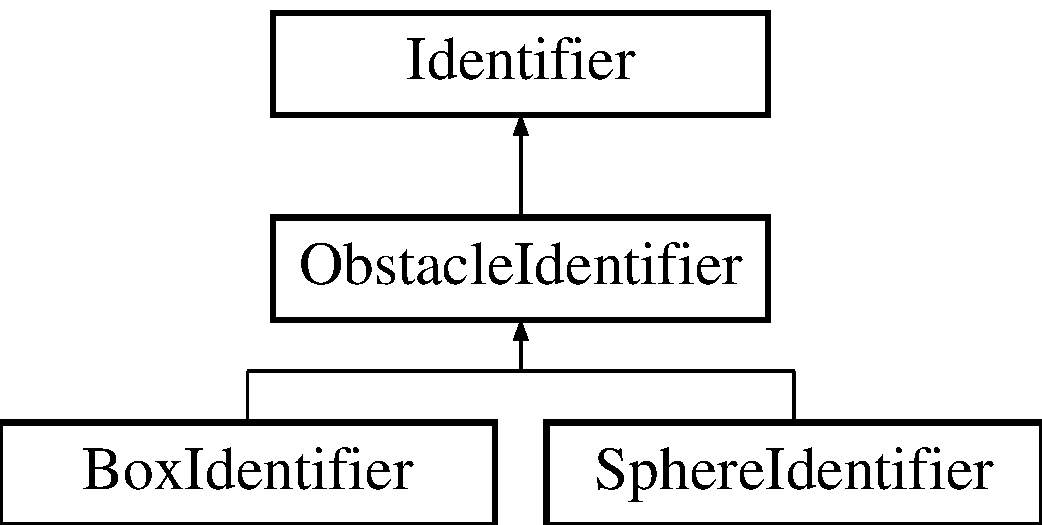
\includegraphics[height=3cm]{class_obstacle_identifier}
\end{center}
\end{figure}
\subsection*{Public Member Functions}
\begin{CompactItemize}
\item 
\hypertarget{class_obstacle_identifier_a9fb5f13b6cf6bdb188be340935e40a4}{
virtual boost::shared\_\-ptr$<$ \hyperlink{class_identifier}{Identifier} $>$ \textbf{clone} () const =0}
\label{class_obstacle_identifier_a9fb5f13b6cf6bdb188be340935e40a4}

\end{CompactItemize}
\subsection*{Protected Member Functions}
\begin{CompactItemize}
\item 
\hypertarget{class_obstacle_identifier_cba46d07cc834e281e891526f3a0f631}{
\textbf{ObstacleIdentifier} (std::size\_\-t id)}
\label{class_obstacle_identifier_cba46d07cc834e281e891526f3a0f631}

\end{CompactItemize}


\subsection{Detailed Description}
Denote ID's of obstacles. 

\begin{Desc}
\item[Author:]Martina Hüllmann \end{Desc}


Definition at line 12 of file obstacle\_\-identifier.h.

The documentation for this class was generated from the following files:\begin{CompactItemize}
\item 
src/Model/obstacle\_\-identifier.h\item 
src/Model/obstacle\_\-identifier.cc\end{CompactItemize}

\hypertarget{class_octree}{
\section{Octree Class Reference}
\label{class_octree}\index{Octree@{Octree}}
}
Implements an \hyperlink{class_octree}{Octree} for WorldObjects.  


{\tt \#include $<$octree.h$>$}

\subsection*{Public Types}
\begin{CompactItemize}
\item 
enum \hyperlink{class_octree_0279a06c2f71637befe827a037c89311}{OctreeNodes} \{ \par
\textbf{TOP\_\-LEFT\_\-FRONT}, 
\textbf{TOP\_\-LEFT\_\-BACK}, 
\textbf{TOP\_\-RIGHT\_\-BACK}, 
\par
\textbf{TOP\_\-RIGHT\_\-FRONT}, 
\textbf{BOTTOM\_\-LEFT\_\-FRONT}, 
\textbf{BOTTOM\_\-LEFT\_\-BACK}, 
\par
\textbf{BOTTOM\_\-RIGHT\_\-BACK}, 
\textbf{BOTTOM\_\-RIGHT\_\-FRONT}
 \}
\begin{CompactList}\small\item\em Gives Names to Child Nodes of the octree instead of numeric values. \item\end{CompactList}\end{CompactItemize}
\subsection*{Public Member Functions}
\begin{CompactItemize}
\item 
\hyperlink{class_octree_5a8d6069e6a7848f8f1df2a4975cd446}{Octree} ()
\begin{CompactList}\small\item\em Set up the \hyperlink{class_octree}{Octree} Node. \item\end{CompactList}\item 
\hypertarget{class_octree_53a9d3f5b99977ece75cc5e00c4e9aed}{
\textbf{Octree} (int max\_\-levels)}
\label{class_octree_53a9d3f5b99977ece75cc5e00c4e9aed}

\item 
\hypertarget{class_octree_9e3744a765883d1d20f345a4336fc639}{
\textbf{Octree} (float min\_\-width)}
\label{class_octree_9e3744a765883d1d20f345a4336fc639}

\item 
\hyperlink{class_octree_1fba0564f41c14943a79fc874e92a60d}{Octree} (int max\_\-levels, float min\_\-width)
\begin{CompactList}\small\item\em Set up the \hyperlink{class_octree}{Octree} Node. \item\end{CompactList}\item 
\hypertarget{class_octree_ed978900fdafcf488b852f15d7690f42}{
void \textbf{destroy\_\-octree} ()}
\label{class_octree_ed978900fdafcf488b852f15d7690f42}

\item 
void \hyperlink{class_octree_d09d7848f637b4322aa94f93217ef686}{scene\_\-dimensions} (const std::vector$<$ boost::shared\_\-ptr$<$ \hyperlink{class_world_object}{WorldObject} $>$ $>$ \&markers, const std::vector$<$ boost::shared\_\-ptr$<$ Obstacle $>$ $>$ \&obstacles, const std::vector$<$ boost::shared\_\-ptr$<$ \hyperlink{class_robot_data}{RobotData} $>$ $>$ \&robot\_\-datas)
\begin{CompactList}\small\item\em This sets the initial width, height and depth for the whole scene. \item\end{CompactList}\item 
Vector3d \hyperlink{class_octree_65c7cdf803bfb02dab9681ff6bc03520}{new\_\-node\_\-center} (Vector3d center, float width, int node\_\-id)
\begin{CompactList}\small\item\em This Method calculates the new center point of a node. \item\end{CompactList}\item 
void \hyperlink{class_octree_7eb807d724b4caa99d723d07c1d1f4a6}{create\_\-node} (const std::vector$<$ boost::shared\_\-ptr$<$ \hyperlink{class_world_object}{WorldObject} $>$ $>$ \&markers, const std::vector$<$ boost::shared\_\-ptr$<$ Obstacle $>$ $>$ \&obstacles, const std::vector$<$ boost::shared\_\-ptr$<$ \hyperlink{class_robot_data}{RobotData} $>$ $>$ \&robot\_\-datas, const Vector3d center, float width)
\item 
void \hyperlink{class_octree_a40e7b86db10838454cf39b3dc04e762}{create\_\-new\_\-node} (const std::vector$<$ boost::shared\_\-ptr$<$ \hyperlink{class_world_object}{WorldObject} $>$ $>$ \&markers, const std::vector$<$ boost::shared\_\-ptr$<$ Obstacle $>$ $>$ \&obstacles, const std::vector$<$ boost::shared\_\-ptr$<$ \hyperlink{class_robot_data}{RobotData} $>$ $>$ \&robot\_\-datas, Vector3d center, float width, int node\_\-id)
\begin{CompactList}\small\item\em This creates a new node. \item\end{CompactList}\item 
void \hyperlink{class_octree_2bb5bd9cce1feeebecd645f893647681}{create\_\-tree} (const std::vector$<$ boost::shared\_\-ptr$<$ \hyperlink{class_world_object}{WorldObject} $>$ $>$ \&markers, const std::vector$<$ boost::shared\_\-ptr$<$ Obstacle $>$ $>$ \&obstacles, const std::vector$<$ boost::shared\_\-ptr$<$ \hyperlink{class_robot_data}{RobotData} $>$ $>$ \&robot\_\-datas)
\begin{CompactList}\small\item\em This is the starting point of the tree creation. \item\end{CompactList}\item 
float \hyperlink{class_octree_2108bbcd5fecadd8e3f072f871c5632c}{calculate\_\-dist\_\-to\_\-node} (const Vector3d \&pos) const 
\begin{CompactList}\small\item\em Calculates the distance to this node from a given point. \item\end{CompactList}\item 
int \hyperlink{class_octree_de868d730ef2ebe1442d0cc65cfc4f39}{point\_\-in\_\-node} (const Vector3d \&pos)
\item 
bool \hyperlink{class_octree_09d72bc24be26e5814e01ee2674545b1}{does\_\-obstacle\_\-fit} (boost::shared\_\-ptr$<$ Obstacle $>$ \&obstacle) const 
\item 
void \hyperlink{class_octree_7c327c632fbbcac0676ccd8dda9d99ce}{assign\_\-objects\_\-to\_\-node} (const std::vector$<$ boost::shared\_\-ptr$<$ \hyperlink{class_world_object}{WorldObject} $>$ $>$ \&markers, const std::vector$<$ boost::shared\_\-ptr$<$ Obstacle $>$ $>$ \&obstacles, const std::vector$<$ boost::shared\_\-ptr$<$ \hyperlink{class_robot_data}{RobotData} $>$ $>$ \&robot\_\-datas)
\item 
void \hyperlink{class_octree_1e97431b76893f009beca8578f365ca9}{add\_\-marker\_\-to\_\-node} (boost::shared\_\-ptr$<$ \hyperlink{class_world_object}{WorldObject} $>$ marker)
\item 
void \hyperlink{class_octree_bf82f696a0f350ad2eae35431e971a66}{add\_\-obstacle\_\-to\_\-node} (boost::shared\_\-ptr$<$ Obstacle $>$ obstacle)
\item 
void \hyperlink{class_octree_c09b4c93c005fd24b6feb35147d6cfd1}{add\_\-robot\_\-data\_\-to\_\-node} (boost::shared\_\-ptr$<$ \hyperlink{class_robot_data}{RobotData} $>$ robot\_\-data)
\item 
std::vector$<$ boost::shared\_\-ptr$<$ \hyperlink{class_world_object}{WorldObject} $>$ $>$ \& \hyperlink{class_octree_b87eff58fb428441817a569e4674a414}{marker\_\-information} ()
\item 
std::vector$<$ boost::shared\_\-ptr$<$ Obstacle $>$ $>$ \& \hyperlink{class_octree_0f5d4b3c958b35605eb5f8ed808dc021}{obstacles} ()
\item 
std::vector$<$ boost::shared\_\-ptr$<$ \hyperlink{class_robot_data}{RobotData} $>$ $>$ \& \hyperlink{class_octree_daef5372a7ebc7e42cc7f3004b68c1ed}{robot\_\-datas} ()
\item 
void \hyperlink{class_octree_9b884a39d8adf578ced6df783d477c4c}{set\_\-parent} (\hyperlink{class_octree}{Octree} $\ast$parent)
\item 
\hyperlink{class_octree}{Octree} \& \hyperlink{class_octree_1aa93bae9b39e49b97f587357747cd17}{parent} ()
\item 
int \hyperlink{class_octree_e6729a08500e8937d91d809db870777c}{level} ()
\item 
Vector3d \hyperlink{class_octree_8a7a88c27aa9a48f6fbdfd6db5faa455}{center} () const 
\item 
int \hyperlink{class_octree_88cb79978d550bdd2699c15fe9879fc4}{object\_\-count} () const 
\item 
float \hyperlink{class_octree_174fc16c8dda632cf8c0ba7bfc9db4b0}{width} () const 
\item 
bool \hyperlink{class_octree_c05628e77200a5243dd1b0d84332ef39}{sub\_\-divided} () const 
\item 
int \hyperlink{class_octree_f514ecc29e3882b0c2e46ccb5ba4fcd9}{max\_\-levels} ()
\item 
float \hyperlink{class_octree_9c9093d2ed7caa8ac16a1f230a66428f}{min\_\-width} ()
\item 
const boost::shared\_\-ptr$<$ \hyperlink{class_octree}{Octree} $>$ \& \hyperlink{class_octree_211c7b90c150193b6124c05229eb2abb}{child} (int child\_\-id)
\end{CompactItemize}
\subsection*{Protected Member Functions}
\begin{CompactItemize}
\item 
void \hyperlink{class_octree_3456b71a9ff5067eed4317fe10947fcf}{set\_\-level} (int level)
\item 
void \hyperlink{class_octree_eb0215c31bf2b52267e0252940812680}{set\_\-max\_\-levels} (int max\_\-level)
\item 
void \hyperlink{class_octree_046a7db4d122f2b8ef6a5188ef78ffda}{set\_\-min\_\-width} (float min\_\-width)
\item 
int \hyperlink{class_octree_a721cdd20e21a952ea04721ae756d091}{determine\_\-obstacle\_\-type} (const boost::shared\_\-ptr$<$ Obstacle $>$ \&obstacle) const 
\begin{CompactList}\small\item\em Helps to determin the type of an obstacle object. \item\end{CompactList}\item 
float \hyperlink{class_octree_295852d7bca479a4abf01c579d2e93ae}{determine\_\-obstacle\_\-max\_\-size} (const boost::shared\_\-ptr$<$ Obstacle $>$ \&obstacle) const 
\begin{CompactList}\small\item\em Returns the maximum size of an obstacle. \item\end{CompactList}\end{CompactItemize}
\subsection*{Private Member Functions}
\begin{CompactItemize}
\item 
\hypertarget{class_octree_311009ce6bc730b736fccde2f3b840d8}{
void \textbf{init\_\-octree} ()}
\label{class_octree_311009ce6bc730b736fccde2f3b840d8}

\end{CompactItemize}
\subsection*{Private Attributes}
\begin{CompactItemize}
\item 
\hyperlink{class_octree}{Octree} $\ast$ \hyperlink{class_octree_513527d29f670449b0a665625d476ad6}{parent\_\-}
\item 
int \hyperlink{class_octree_3955482b438c39aef803253592306217}{level\_\-}
\item 
int \hyperlink{class_octree_1b29e2ff7de0ce212008fc928de2e8c0}{max\_\-levels\_\-}
\item 
float \hyperlink{class_octree_d8300c6fe2f72671675b351e8b4e65db}{min\_\-width\_\-}
\item 
bool \hyperlink{class_octree_1ff3eebef24edecea4359fdaa994d26d}{sub\_\-divided\_\-}
\item 
float \hyperlink{class_octree_8f8660a65257ea4368c6ba2e57df86fc}{width\_\-}
\item 
int \hyperlink{class_octree_0faf7b0d6e445aee6e6954d4efdafcf9}{object\_\-count\_\-}
\item 
Vector3d \hyperlink{class_octree_d1830408734e4435f934a6cb31a0c8a4}{center\_\-}
\item 
std::vector$<$ boost::shared\_\-ptr$<$ \hyperlink{class_world_object}{WorldObject} $>$ $>$ \hyperlink{class_octree_420b03d97b1631a2809b3b4929a84e89}{markers\_\-}
\item 
std::vector$<$ boost::shared\_\-ptr$<$ Obstacle $>$ $>$ \hyperlink{class_octree_7ba27f0c60cc3eceb10799bcc43e8acf}{obstacles\_\-}
\item 
std::vector$<$ boost::shared\_\-ptr$<$ \hyperlink{class_robot_data}{RobotData} $>$ $>$ \hyperlink{class_octree_f93af4c2615db522f4496fd050a5b61b}{robot\_\-datas\_\-}
\item 
boost::shared\_\-ptr$<$ \hyperlink{class_octree}{Octree} $>$ \hyperlink{class_octree_a7b4d7aa295f945512b9e39d8fd2d5d6}{octree\_\-nodes\_\-} \mbox{[}8\mbox{]}
\end{CompactItemize}
\subsection*{Friends}
\begin{CompactItemize}
\item 
\hypertarget{class_octree_836eb2cdddfa75db7fe8368e211bbe65}{
class \hyperlink{class_octree_836eb2cdddfa75db7fe8368e211bbe65}{OctreeUtilities}}
\label{class_octree_836eb2cdddfa75db7fe8368e211bbe65}

\end{CompactItemize}


\subsection{Detailed Description}
Implements an \hyperlink{class_octree}{Octree} for WorldObjects. 

\begin{Desc}
\item[Author:]Kamil Swierkot TODO: Describe how to use this class.... \end{Desc}


Definition at line 30 of file octree.h.

\subsection{Constructor \& Destructor Documentation}
\hypertarget{class_octree_5a8d6069e6a7848f8f1df2a4975cd446}{
\index{Octree@{Octree}!Octree@{Octree}}
\index{Octree@{Octree}!Octree@{Octree}}
\subsubsection[Octree]{\setlength{\rightskip}{0pt plus 5cm}Octree::Octree ()}}
\label{class_octree_5a8d6069e6a7848f8f1df2a4975cd446}


Set up the \hyperlink{class_octree}{Octree} Node. 

max\_\-levels\_\- is set to 20000 and min\_\-width\_\- is set to 0. 

Definition at line 23 of file octree.cc.

References max\_\-levels\_\-, and min\_\-width\_\-.

Referenced by create\_\-new\_\-node().\hypertarget{class_octree_1fba0564f41c14943a79fc874e92a60d}{
\index{Octree@{Octree}!Octree@{Octree}}
\index{Octree@{Octree}!Octree@{Octree}}
\subsubsection[Octree]{\setlength{\rightskip}{0pt plus 5cm}Octree::Octree (int {\em max\_\-levels}, \/  float {\em min\_\-width})}}
\label{class_octree_1fba0564f41c14943a79fc874e92a60d}


Set up the \hyperlink{class_octree}{Octree} Node. 

\begin{Desc}
\item[Parameters:]
\begin{description}
\item[{\em max\_\-levels}]Used to set the maximum depth of the \hyperlink{class_octree}{Octree} \item[{\em min\_\-width}]Used to set the min\_\-width of an octree node \end{description}
\end{Desc}


Definition at line 45 of file octree.cc.

\subsection{Member Function Documentation}
\hypertarget{class_octree_d09d7848f637b4322aa94f93217ef686}{
\index{Octree@{Octree}!scene\_\-dimensions@{scene\_\-dimensions}}
\index{scene\_\-dimensions@{scene\_\-dimensions}!Octree@{Octree}}
\subsubsection[scene\_\-dimensions]{\setlength{\rightskip}{0pt plus 5cm}void Octree::scene\_\-dimensions (const std::vector$<$ boost::shared\_\-ptr$<$ {\bf WorldObject} $>$ $>$ \& {\em markers}, \/  const std::vector$<$ boost::shared\_\-ptr$<$ Obstacle $>$ $>$ \& {\em obstacles}, \/  const std::vector$<$ boost::shared\_\-ptr$<$ {\bf RobotData} $>$ $>$ \& {\em robot\_\-datas})}}
\label{class_octree_d09d7848f637b4322aa94f93217ef686}


This sets the initial width, height and depth for the whole scene. 

\begin{Desc}
\item[Parameters:]
\begin{description}
\item[{\em markers}]The marker object in an vector of shared\_\-ptr \item[{\em obstacles}]The obstacles in an vector of shared\_\-ptr \item[{\em robot\_\-datas}]The robot\_\-datas in an vector of shared\_\-ptr \end{description}
\end{Desc}


Definition at line 97 of file octree.cc.

References center\_\-, determine\_\-obstacle\_\-max\_\-size(), obstacles(), robot\_\-datas(), and width\_\-.

Referenced by create\_\-tree().\hypertarget{class_octree_65c7cdf803bfb02dab9681ff6bc03520}{
\index{Octree@{Octree}!new\_\-node\_\-center@{new\_\-node\_\-center}}
\index{new\_\-node\_\-center@{new\_\-node\_\-center}!Octree@{Octree}}
\subsubsection[new\_\-node\_\-center]{\setlength{\rightskip}{0pt plus 5cm}Vector3d Octree::new\_\-node\_\-center (Vector3d {\em center}, \/  float {\em width}, \/  int {\em node\_\-id})}}
\label{class_octree_65c7cdf803bfb02dab9681ff6bc03520}


This Method calculates the new center point of a node. 

This takes in the previous nodes center, width and which node ID that will be subdivided. The Result is the center of the new node. \begin{Desc}
\item[Parameters:]
\begin{description}
\item[{\em center}]The center of the parent node \item[{\em width}]The width of the \hyperlink{class_octree}{Octree} Node box. \item[{\em node\_\-id}]The ID of the node \end{description}
\end{Desc}


Definition at line 234 of file octree.cc.

References center().

Referenced by create\_\-new\_\-node(), and create\_\-node().\hypertarget{class_octree_7eb807d724b4caa99d723d07c1d1f4a6}{
\index{Octree@{Octree}!create\_\-node@{create\_\-node}}
\index{create\_\-node@{create\_\-node}!Octree@{Octree}}
\subsubsection[create\_\-node]{\setlength{\rightskip}{0pt plus 5cm}void Octree::create\_\-node (const std::vector$<$ boost::shared\_\-ptr$<$ {\bf WorldObject} $>$ $>$ \& {\em markers}, \/  const std::vector$<$ boost::shared\_\-ptr$<$ Obstacle $>$ $>$ \& {\em obstacles}, \/  const std::vector$<$ boost::shared\_\-ptr$<$ {\bf RobotData} $>$ $>$ \& {\em robot\_\-datas}, \/  const Vector3d {\em center}, \/  float {\em width})}}
\label{class_octree_7eb807d724b4caa99d723d07c1d1f4a6}


This subdivides a node depending on the objects and node width

\begin{Desc}
\item[Parameters:]
\begin{description}
\item[{\em markers}]the markers to store in this subtree \item[{\em obstacles}]the obstacles to store in this subtree \item[{\em robot\_\-datas}]the robot\_\-datas to store in this subtree \item[{\em center}]the center point of this node \item[{\em width}]the width of this node \end{description}
\end{Desc}


Definition at line 377 of file octree.cc.

References assign\_\-objects\_\-to\_\-node(), center(), center\_\-, create\_\-new\_\-node(), determine\_\-obstacle\_\-max\_\-size(), level\_\-, max\_\-levels\_\-, min\_\-width\_\-, new\_\-node\_\-center(), object\_\-count(), object\_\-count\_\-, obstacles(), obstacles\_\-, octree\_\-nodes\_\-, robot\_\-datas(), sub\_\-divided\_\-, and width\_\-.

Referenced by create\_\-tree().\hypertarget{class_octree_a40e7b86db10838454cf39b3dc04e762}{
\index{Octree@{Octree}!create\_\-new\_\-node@{create\_\-new\_\-node}}
\index{create\_\-new\_\-node@{create\_\-new\_\-node}!Octree@{Octree}}
\subsubsection[create\_\-new\_\-node]{\setlength{\rightskip}{0pt plus 5cm}void Octree::create\_\-new\_\-node (const std::vector$<$ boost::shared\_\-ptr$<$ {\bf WorldObject} $>$ $>$ \& {\em markers}, \/  const std::vector$<$ boost::shared\_\-ptr$<$ Obstacle $>$ $>$ \& {\em obstacles}, \/  const std::vector$<$ boost::shared\_\-ptr$<$ {\bf RobotData} $>$ $>$ \& {\em robot\_\-datas}, \/  Vector3d {\em center}, \/  float {\em width}, \/  int {\em node\_\-id})}}
\label{class_octree_a40e7b86db10838454cf39b3dc04e762}


This creates a new node. 

\begin{Desc}
\item[Parameters:]
\begin{description}
\item[{\em markers}]The Markers to be stored in this subtree \item[{\em obstacles}]The obstacles to be stored in this subtree \item[{\em robot\_\-datas}]The robot datas to be stored in this subtree \item[{\em center}]The center point of the new node \item[{\em width}]the width of the bounding box \end{description}
\end{Desc}


Definition at line 332 of file octree.cc.

References level\_\-, max\_\-levels\_\-, min\_\-width\_\-, new\_\-node\_\-center(), obstacles(), Octree(), octree\_\-nodes\_\-, and robot\_\-datas().

Referenced by create\_\-node().\hypertarget{class_octree_2bb5bd9cce1feeebecd645f893647681}{
\index{Octree@{Octree}!create\_\-tree@{create\_\-tree}}
\index{create\_\-tree@{create\_\-tree}!Octree@{Octree}}
\subsubsection[create\_\-tree]{\setlength{\rightskip}{0pt plus 5cm}void Octree::create\_\-tree (const std::vector$<$ boost::shared\_\-ptr$<$ {\bf WorldObject} $>$ $>$ \& {\em markers}, \/  const std::vector$<$ boost::shared\_\-ptr$<$ Obstacle $>$ $>$ \& {\em obstacles}, \/  const std::vector$<$ boost::shared\_\-ptr$<$ {\bf RobotData} $>$ $>$ \& {\em robot\_\-datas})}}
\label{class_octree_2bb5bd9cce1feeebecd645f893647681}


This is the starting point of the tree creation. 

\begin{Desc}
\item[Parameters:]
\begin{description}
\item[{\em markers}]the markers to be stored in this tree \item[{\em obstacles}]the obstacles to be stored in this tree \item[{\em robot\_\-datas}]the robot datas to be stored in this tree \end{description}
\end{Desc}


Definition at line 877 of file octree.cc.

References center\_\-, create\_\-node(), obstacles(), robot\_\-datas(), scene\_\-dimensions(), and width\_\-.\hypertarget{class_octree_2108bbcd5fecadd8e3f072f871c5632c}{
\index{Octree@{Octree}!calculate\_\-dist\_\-to\_\-node@{calculate\_\-dist\_\-to\_\-node}}
\index{calculate\_\-dist\_\-to\_\-node@{calculate\_\-dist\_\-to\_\-node}!Octree@{Octree}}
\subsubsection[calculate\_\-dist\_\-to\_\-node]{\setlength{\rightskip}{0pt plus 5cm}float Octree::calculate\_\-dist\_\-to\_\-node (const Vector3d \& {\em pos}) const}}
\label{class_octree_2108bbcd5fecadd8e3f072f871c5632c}


Calculates the distance to this node from a given point. 

\begin{Desc}
\item[Parameters:]
\begin{description}
\item[{\em pos}]The position \end{description}
\end{Desc}
\begin{Desc}
\item[Returns:]Returns the distance to this node from the given point \end{Desc}


Definition at line 756 of file octree.cc.

References center\_\-, and width\_\-.\hypertarget{class_octree_de868d730ef2ebe1442d0cc65cfc4f39}{
\index{Octree@{Octree}!point\_\-in\_\-node@{point\_\-in\_\-node}}
\index{point\_\-in\_\-node@{point\_\-in\_\-node}!Octree@{Octree}}
\subsubsection[point\_\-in\_\-node]{\setlength{\rightskip}{0pt plus 5cm}int Octree::point\_\-in\_\-node (const Vector3d \& {\em pos})}}
\label{class_octree_de868d730ef2ebe1442d0cc65cfc4f39}


Returns the index of the child node in which the point would belong to

\begin{Desc}
\item[Parameters:]
\begin{description}
\item[{\em pos}]The position of the point \end{description}
\end{Desc}


Definition at line 825 of file octree.cc.

References center\_\-.\hypertarget{class_octree_09d72bc24be26e5814e01ee2674545b1}{
\index{Octree@{Octree}!does\_\-obstacle\_\-fit@{does\_\-obstacle\_\-fit}}
\index{does\_\-obstacle\_\-fit@{does\_\-obstacle\_\-fit}!Octree@{Octree}}
\subsubsection[does\_\-obstacle\_\-fit]{\setlength{\rightskip}{0pt plus 5cm}bool Octree::does\_\-obstacle\_\-fit (boost::shared\_\-ptr$<$ Obstacle $>$ \& {\em obstacle}) const}}
\label{class_octree_09d72bc24be26e5814e01ee2674545b1}


Returns whether an obstacle would fit into this node or not

\begin{Desc}
\item[Parameters:]
\begin{description}
\item[{\em obstacle}]the obstacle \end{description}
\end{Desc}


Definition at line 769 of file octree.cc.

References determine\_\-obstacle\_\-max\_\-size().\hypertarget{class_octree_7c327c632fbbcac0676ccd8dda9d99ce}{
\index{Octree@{Octree}!assign\_\-objects\_\-to\_\-node@{assign\_\-objects\_\-to\_\-node}}
\index{assign\_\-objects\_\-to\_\-node@{assign\_\-objects\_\-to\_\-node}!Octree@{Octree}}
\subsubsection[assign\_\-objects\_\-to\_\-node]{\setlength{\rightskip}{0pt plus 5cm}void Octree::assign\_\-objects\_\-to\_\-node (const std::vector$<$ boost::shared\_\-ptr$<$ {\bf WorldObject} $>$ $>$ \& {\em markers}, \/  const std::vector$<$ boost::shared\_\-ptr$<$ Obstacle $>$ $>$ \& {\em obstacles}, \/  const std::vector$<$ boost::shared\_\-ptr$<$ {\bf RobotData} $>$ $>$ \& {\em robot\_\-datas})}}
\label{class_octree_7c327c632fbbcac0676ccd8dda9d99ce}


This method allows to add objects to the octree.

\begin{Desc}
\item[Parameters:]
\begin{description}
\item[{\em markers}]The new marker objects \item[{\em obstacles}]The new obstacles \item[{\em robot\_\-datas}]The new robot\_\-datas \end{description}
\end{Desc}


Definition at line 888 of file octree.cc.

References markers\_\-, obstacles(), obstacles\_\-, robot\_\-datas(), and robot\_\-datas\_\-.

Referenced by create\_\-node().\hypertarget{class_octree_1e97431b76893f009beca8578f365ca9}{
\index{Octree@{Octree}!add\_\-marker\_\-to\_\-node@{add\_\-marker\_\-to\_\-node}}
\index{add\_\-marker\_\-to\_\-node@{add\_\-marker\_\-to\_\-node}!Octree@{Octree}}
\subsubsection[add\_\-marker\_\-to\_\-node]{\setlength{\rightskip}{0pt plus 5cm}void Octree::add\_\-marker\_\-to\_\-node (boost::shared\_\-ptr$<$ {\bf WorldObject} $>$ {\em marker})}}
\label{class_octree_1e97431b76893f009beca8578f365ca9}


This method allows to add a marker to this node

\begin{Desc}
\item[Parameters:]
\begin{description}
\item[{\em marker}]The marker to add to this node \end{description}
\end{Desc}


Definition at line 897 of file octree.cc.

References markers\_\-.\hypertarget{class_octree_bf82f696a0f350ad2eae35431e971a66}{
\index{Octree@{Octree}!add\_\-obstacle\_\-to\_\-node@{add\_\-obstacle\_\-to\_\-node}}
\index{add\_\-obstacle\_\-to\_\-node@{add\_\-obstacle\_\-to\_\-node}!Octree@{Octree}}
\subsubsection[add\_\-obstacle\_\-to\_\-node]{\setlength{\rightskip}{0pt plus 5cm}void Octree::add\_\-obstacle\_\-to\_\-node (boost::shared\_\-ptr$<$ Obstacle $>$ {\em obstacle})}}
\label{class_octree_bf82f696a0f350ad2eae35431e971a66}


This method allows to add an obstacle to this node

\begin{Desc}
\item[Parameters:]
\begin{description}
\item[{\em obstacle}]The obstacle to add to this node \end{description}
\end{Desc}


Definition at line 903 of file octree.cc.

References obstacles\_\-.\hypertarget{class_octree_c09b4c93c005fd24b6feb35147d6cfd1}{
\index{Octree@{Octree}!add\_\-robot\_\-data\_\-to\_\-node@{add\_\-robot\_\-data\_\-to\_\-node}}
\index{add\_\-robot\_\-data\_\-to\_\-node@{add\_\-robot\_\-data\_\-to\_\-node}!Octree@{Octree}}
\subsubsection[add\_\-robot\_\-data\_\-to\_\-node]{\setlength{\rightskip}{0pt plus 5cm}void Octree::add\_\-robot\_\-data\_\-to\_\-node (boost::shared\_\-ptr$<$ {\bf RobotData} $>$ {\em robot\_\-data})}}
\label{class_octree_c09b4c93c005fd24b6feb35147d6cfd1}


This method allows to add a robot data to this node

\begin{Desc}
\item[Parameters:]
\begin{description}
\item[{\em robot\_\-data}]the new robot\_\-data to add to this node \end{description}
\end{Desc}


Definition at line 909 of file octree.cc.

References robot\_\-datas\_\-.\hypertarget{class_octree_b87eff58fb428441817a569e4674a414}{
\index{Octree@{Octree}!marker\_\-information@{marker\_\-information}}
\index{marker\_\-information@{marker\_\-information}!Octree@{Octree}}
\subsubsection[marker\_\-information]{\setlength{\rightskip}{0pt plus 5cm}std::vector$<$ boost::shared\_\-ptr$<${\bf WorldObject}$>$ $>$\& Octree::marker\_\-information ()\hspace{0.3cm}{\tt  \mbox{[}inline\mbox{]}}}}
\label{class_octree_b87eff58fb428441817a569e4674a414}


Returns the marker stored in this node. 

Definition at line 205 of file octree.h.

References markers\_\-.\hypertarget{class_octree_0f5d4b3c958b35605eb5f8ed808dc021}{
\index{Octree@{Octree}!obstacles@{obstacles}}
\index{obstacles@{obstacles}!Octree@{Octree}}
\subsubsection[obstacles]{\setlength{\rightskip}{0pt plus 5cm}std::vector$<$ boost::shared\_\-ptr$<$Obstacle$>$ $>$\& Octree::obstacles ()\hspace{0.3cm}{\tt  \mbox{[}inline\mbox{]}}}}
\label{class_octree_0f5d4b3c958b35605eb5f8ed808dc021}


Returns the obstacles stored in this node. 

Definition at line 212 of file octree.h.

References obstacles\_\-.

Referenced by assign\_\-objects\_\-to\_\-node(), create\_\-new\_\-node(), create\_\-node(), create\_\-tree(), and scene\_\-dimensions().\hypertarget{class_octree_daef5372a7ebc7e42cc7f3004b68c1ed}{
\index{Octree@{Octree}!robot\_\-datas@{robot\_\-datas}}
\index{robot\_\-datas@{robot\_\-datas}!Octree@{Octree}}
\subsubsection[robot\_\-datas]{\setlength{\rightskip}{0pt plus 5cm}std::vector$<$ boost::shared\_\-ptr$<${\bf RobotData}$>$ $>$\& Octree::robot\_\-datas ()\hspace{0.3cm}{\tt  \mbox{[}inline\mbox{]}}}}
\label{class_octree_daef5372a7ebc7e42cc7f3004b68c1ed}


Returns the robot datas stored in this node. 

Definition at line 219 of file octree.h.

References robot\_\-datas\_\-.

Referenced by assign\_\-objects\_\-to\_\-node(), create\_\-new\_\-node(), create\_\-node(), create\_\-tree(), and scene\_\-dimensions().\hypertarget{class_octree_9b884a39d8adf578ced6df783d477c4c}{
\index{Octree@{Octree}!set\_\-parent@{set\_\-parent}}
\index{set\_\-parent@{set\_\-parent}!Octree@{Octree}}
\subsubsection[set\_\-parent]{\setlength{\rightskip}{0pt plus 5cm}void Octree::set\_\-parent ({\bf Octree} $\ast$ {\em parent})\hspace{0.3cm}{\tt  \mbox{[}inline\mbox{]}}}}
\label{class_octree_9b884a39d8adf578ced6df783d477c4c}


This sets the parent of this node

\begin{Desc}
\item[Parameters:]
\begin{description}
\item[{\em parent}]A pointer to the parent of this node \end{description}
\end{Desc}


Definition at line 228 of file octree.h.

References parent\_\-.\hypertarget{class_octree_1aa93bae9b39e49b97f587357747cd17}{
\index{Octree@{Octree}!parent@{parent}}
\index{parent@{parent}!Octree@{Octree}}
\subsubsection[parent]{\setlength{\rightskip}{0pt plus 5cm}{\bf Octree}\& Octree::parent ()\hspace{0.3cm}{\tt  \mbox{[}inline\mbox{]}}}}
\label{class_octree_1aa93bae9b39e49b97f587357747cd17}


Returns the parent of this node. This is node a boost::shared\_\-ptr because the child nodes get destroyed before their parent. 

Definition at line 237 of file octree.h.

References parent\_\-.\hypertarget{class_octree_e6729a08500e8937d91d809db870777c}{
\index{Octree@{Octree}!level@{level}}
\index{level@{level}!Octree@{Octree}}
\subsubsection[level]{\setlength{\rightskip}{0pt plus 5cm}int Octree::level ()\hspace{0.3cm}{\tt  \mbox{[}inline\mbox{]}}}}
\label{class_octree_e6729a08500e8937d91d809db870777c}


Returns the depth of this node in the octree 

Definition at line 244 of file octree.h.

References level\_\-.\hypertarget{class_octree_8a7a88c27aa9a48f6fbdfd6db5faa455}{
\index{Octree@{Octree}!center@{center}}
\index{center@{center}!Octree@{Octree}}
\subsubsection[center]{\setlength{\rightskip}{0pt plus 5cm}Vector3d Octree::center () const\hspace{0.3cm}{\tt  \mbox{[}inline\mbox{]}}}}
\label{class_octree_8a7a88c27aa9a48f6fbdfd6db5faa455}


This returns the center of this node 

Definition at line 251 of file octree.h.

References center\_\-.

Referenced by create\_\-node(), and new\_\-node\_\-center().\hypertarget{class_octree_88cb79978d550bdd2699c15fe9879fc4}{
\index{Octree@{Octree}!object\_\-count@{object\_\-count}}
\index{object\_\-count@{object\_\-count}!Octree@{Octree}}
\subsubsection[object\_\-count]{\setlength{\rightskip}{0pt plus 5cm}int Octree::object\_\-count () const\hspace{0.3cm}{\tt  \mbox{[}inline\mbox{]}}}}
\label{class_octree_88cb79978d550bdd2699c15fe9879fc4}


This return the number of objects which were stored in this node 

Definition at line 258 of file octree.h.

References object\_\-count\_\-.

Referenced by create\_\-node().\hypertarget{class_octree_174fc16c8dda632cf8c0ba7bfc9db4b0}{
\index{Octree@{Octree}!width@{width}}
\index{width@{width}!Octree@{Octree}}
\subsubsection[width]{\setlength{\rightskip}{0pt plus 5cm}float Octree::width () const\hspace{0.3cm}{\tt  \mbox{[}inline\mbox{]}}}}
\label{class_octree_174fc16c8dda632cf8c0ba7bfc9db4b0}


This returns the width of this node (since it's a cube the height and depth are the same) 

Definition at line 265 of file octree.h.

References width\_\-.\hypertarget{class_octree_c05628e77200a5243dd1b0d84332ef39}{
\index{Octree@{Octree}!sub\_\-divided@{sub\_\-divided}}
\index{sub\_\-divided@{sub\_\-divided}!Octree@{Octree}}
\subsubsection[sub\_\-divided]{\setlength{\rightskip}{0pt plus 5cm}bool Octree::sub\_\-divided () const\hspace{0.3cm}{\tt  \mbox{[}inline\mbox{]}}}}
\label{class_octree_c05628e77200a5243dd1b0d84332ef39}


This return whether the node is subdivided or not. If a node is subdivided, then it has all eight children. 

Definition at line 274 of file octree.h.

References sub\_\-divided\_\-.\hypertarget{class_octree_f514ecc29e3882b0c2e46ccb5ba4fcd9}{
\index{Octree@{Octree}!max\_\-levels@{max\_\-levels}}
\index{max\_\-levels@{max\_\-levels}!Octree@{Octree}}
\subsubsection[max\_\-levels]{\setlength{\rightskip}{0pt plus 5cm}int Octree::max\_\-levels ()\hspace{0.3cm}{\tt  \mbox{[}inline\mbox{]}}}}
\label{class_octree_f514ecc29e3882b0c2e46ccb5ba4fcd9}


Returns the maximal depth of this octree 

Definition at line 280 of file octree.h.

References max\_\-levels\_\-.\hypertarget{class_octree_9c9093d2ed7caa8ac16a1f230a66428f}{
\index{Octree@{Octree}!min\_\-width@{min\_\-width}}
\index{min\_\-width@{min\_\-width}!Octree@{Octree}}
\subsubsection[min\_\-width]{\setlength{\rightskip}{0pt plus 5cm}float Octree::min\_\-width ()\hspace{0.3cm}{\tt  \mbox{[}inline\mbox{]}}}}
\label{class_octree_9c9093d2ed7caa8ac16a1f230a66428f}


Returns the minimal width of a node in this octree. 

Definition at line 285 of file octree.h.

References min\_\-width\_\-.\hypertarget{class_octree_211c7b90c150193b6124c05229eb2abb}{
\index{Octree@{Octree}!child@{child}}
\index{child@{child}!Octree@{Octree}}
\subsubsection[child]{\setlength{\rightskip}{0pt plus 5cm}const boost::shared\_\-ptr$<${\bf Octree}$>$\& Octree::child (int {\em child\_\-id})\hspace{0.3cm}{\tt  \mbox{[}inline\mbox{]}}}}
\label{class_octree_211c7b90c150193b6124c05229eb2abb}


Returns a child node.

\begin{Desc}
\item[Parameters:]
\begin{description}
\item[{\em child\_\-id}]The number of the child. Values in between 0 and 7 are legal numbers \end{description}
\end{Desc}


Definition at line 292 of file octree.h.

References octree\_\-nodes\_\-.\hypertarget{class_octree_3456b71a9ff5067eed4317fe10947fcf}{
\index{Octree@{Octree}!set\_\-level@{set\_\-level}}
\index{set\_\-level@{set\_\-level}!Octree@{Octree}}
\subsubsection[set\_\-level]{\setlength{\rightskip}{0pt plus 5cm}void Octree::set\_\-level (int {\em level})\hspace{0.3cm}{\tt  \mbox{[}inline, protected\mbox{]}}}}
\label{class_octree_3456b71a9ff5067eed4317fe10947fcf}


Sets the actual depth of this node. \begin{Desc}
\item[Parameters:]
\begin{description}
\item[{\em level}]The depth of this node \end{description}
\end{Desc}


Definition at line 302 of file octree.h.

References level\_\-.\hypertarget{class_octree_eb0215c31bf2b52267e0252940812680}{
\index{Octree@{Octree}!set\_\-max\_\-levels@{set\_\-max\_\-levels}}
\index{set\_\-max\_\-levels@{set\_\-max\_\-levels}!Octree@{Octree}}
\subsubsection[set\_\-max\_\-levels]{\setlength{\rightskip}{0pt plus 5cm}void Octree::set\_\-max\_\-levels (int {\em max\_\-level})\hspace{0.3cm}{\tt  \mbox{[}inline, protected\mbox{]}}}}
\label{class_octree_eb0215c31bf2b52267e0252940812680}


Sets the max depth of the tree \begin{Desc}
\item[Parameters:]
\begin{description}
\item[{\em max\_\-level}]The maximal depth of the tree. \end{description}
\end{Desc}


Definition at line 310 of file octree.h.

References max\_\-levels\_\-.\hypertarget{class_octree_046a7db4d122f2b8ef6a5188ef78ffda}{
\index{Octree@{Octree}!set\_\-min\_\-width@{set\_\-min\_\-width}}
\index{set\_\-min\_\-width@{set\_\-min\_\-width}!Octree@{Octree}}
\subsubsection[set\_\-min\_\-width]{\setlength{\rightskip}{0pt plus 5cm}void Octree::set\_\-min\_\-width (float {\em min\_\-width})\hspace{0.3cm}{\tt  \mbox{[}inline, protected\mbox{]}}}}
\label{class_octree_046a7db4d122f2b8ef6a5188ef78ffda}


Sets the minimal width of a node. \begin{Desc}
\item[Parameters:]
\begin{description}
\item[{\em min\_\-width}]The minimal width of a node. \end{description}
\end{Desc}


Definition at line 316 of file octree.h.

References min\_\-width\_\-.\hypertarget{class_octree_a721cdd20e21a952ea04721ae756d091}{
\index{Octree@{Octree}!determine\_\-obstacle\_\-type@{determine\_\-obstacle\_\-type}}
\index{determine\_\-obstacle\_\-type@{determine\_\-obstacle\_\-type}!Octree@{Octree}}
\subsubsection[determine\_\-obstacle\_\-type]{\setlength{\rightskip}{0pt plus 5cm}int Octree::determine\_\-obstacle\_\-type (const boost::shared\_\-ptr$<$ Obstacle $>$ \& {\em obstacle}) const\hspace{0.3cm}{\tt  \mbox{[}protected\mbox{]}}}}
\label{class_octree_a721cdd20e21a952ea04721ae756d091}


Helps to determin the type of an obstacle object. 

\begin{Desc}
\item[Parameters:]
\begin{description}
\item[{\em obstacle}]The obstacle to retrieve the real type of \end{description}
\end{Desc}
\begin{Desc}
\item[Returns:]The type of the obstacle: 1 \hyperlink{class_box}{Box}, 2 \hyperlink{class_sphere}{Sphere} \end{Desc}


Definition at line 780 of file octree.cc.

Referenced by determine\_\-obstacle\_\-max\_\-size().\hypertarget{class_octree_295852d7bca479a4abf01c579d2e93ae}{
\index{Octree@{Octree}!determine\_\-obstacle\_\-max\_\-size@{determine\_\-obstacle\_\-max\_\-size}}
\index{determine\_\-obstacle\_\-max\_\-size@{determine\_\-obstacle\_\-max\_\-size}!Octree@{Octree}}
\subsubsection[determine\_\-obstacle\_\-max\_\-size]{\setlength{\rightskip}{0pt plus 5cm}float Octree::determine\_\-obstacle\_\-max\_\-size (const boost::shared\_\-ptr$<$ Obstacle $>$ \& {\em obstacle}) const\hspace{0.3cm}{\tt  \mbox{[}protected\mbox{]}}}}
\label{class_octree_295852d7bca479a4abf01c579d2e93ae}


Returns the maximum size of an obstacle. 

\begin{Desc}
\item[Parameters:]
\begin{description}
\item[{\em obstacle}]the obstacle \end{description}
\end{Desc}


Definition at line 792 of file octree.cc.

References Box::depth(), determine\_\-obstacle\_\-type(), Box::height(), Sphere::radius(), and Box::width().

Referenced by create\_\-node(), does\_\-obstacle\_\-fit(), and scene\_\-dimensions().

\subsection{Member Data Documentation}
\hypertarget{class_octree_513527d29f670449b0a665625d476ad6}{
\index{Octree@{Octree}!parent\_\-@{parent\_\-}}
\index{parent\_\-@{parent\_\-}!Octree@{Octree}}
\subsubsection[parent\_\-]{\setlength{\rightskip}{0pt plus 5cm}{\bf Octree}$\ast$ {\bf Octree::parent\_\-}\hspace{0.3cm}{\tt  \mbox{[}private\mbox{]}}}}
\label{class_octree_513527d29f670449b0a665625d476ad6}


this stores an pointer to its parent. 

Definition at line 342 of file octree.h.

Referenced by parent(), and set\_\-parent().\hypertarget{class_octree_3955482b438c39aef803253592306217}{
\index{Octree@{Octree}!level\_\-@{level\_\-}}
\index{level\_\-@{level\_\-}!Octree@{Octree}}
\subsubsection[level\_\-]{\setlength{\rightskip}{0pt plus 5cm}int {\bf Octree::level\_\-}\hspace{0.3cm}{\tt  \mbox{[}private\mbox{]}}}}
\label{class_octree_3955482b438c39aef803253592306217}


The depth of this node. 

Definition at line 347 of file octree.h.

Referenced by create\_\-new\_\-node(), create\_\-node(), level(), and set\_\-level().\hypertarget{class_octree_1b29e2ff7de0ce212008fc928de2e8c0}{
\index{Octree@{Octree}!max\_\-levels\_\-@{max\_\-levels\_\-}}
\index{max\_\-levels\_\-@{max\_\-levels\_\-}!Octree@{Octree}}
\subsubsection[max\_\-levels\_\-]{\setlength{\rightskip}{0pt plus 5cm}int {\bf Octree::max\_\-levels\_\-}\hspace{0.3cm}{\tt  \mbox{[}private\mbox{]}}}}
\label{class_octree_1b29e2ff7de0ce212008fc928de2e8c0}


The maximal depth of this tree 

Definition at line 351 of file octree.h.

Referenced by create\_\-new\_\-node(), create\_\-node(), max\_\-levels(), Octree(), and set\_\-max\_\-levels().\hypertarget{class_octree_d8300c6fe2f72671675b351e8b4e65db}{
\index{Octree@{Octree}!min\_\-width\_\-@{min\_\-width\_\-}}
\index{min\_\-width\_\-@{min\_\-width\_\-}!Octree@{Octree}}
\subsubsection[min\_\-width\_\-]{\setlength{\rightskip}{0pt plus 5cm}float {\bf Octree::min\_\-width\_\-}\hspace{0.3cm}{\tt  \mbox{[}private\mbox{]}}}}
\label{class_octree_d8300c6fe2f72671675b351e8b4e65db}


The minimum size of an node 

Definition at line 355 of file octree.h.

Referenced by create\_\-new\_\-node(), create\_\-node(), min\_\-width(), Octree(), and set\_\-min\_\-width().\hypertarget{class_octree_1ff3eebef24edecea4359fdaa994d26d}{
\index{Octree@{Octree}!sub\_\-divided\_\-@{sub\_\-divided\_\-}}
\index{sub\_\-divided\_\-@{sub\_\-divided\_\-}!Octree@{Octree}}
\subsubsection[sub\_\-divided\_\-]{\setlength{\rightskip}{0pt plus 5cm}bool {\bf Octree::sub\_\-divided\_\-}\hspace{0.3cm}{\tt  \mbox{[}private\mbox{]}}}}
\label{class_octree_1ff3eebef24edecea4359fdaa994d26d}


This tells whether the node has been subdivided or not. If this has been set to true, there won't be any robots and markers saved in this node 

Definition at line 361 of file octree.h.

Referenced by create\_\-node(), and sub\_\-divided().\hypertarget{class_octree_8f8660a65257ea4368c6ba2e57df86fc}{
\index{Octree@{Octree}!width\_\-@{width\_\-}}
\index{width\_\-@{width\_\-}!Octree@{Octree}}
\subsubsection[width\_\-]{\setlength{\rightskip}{0pt plus 5cm}float {\bf Octree::width\_\-}\hspace{0.3cm}{\tt  \mbox{[}private\mbox{]}}}}
\label{class_octree_8f8660a65257ea4368c6ba2e57df86fc}


This is the size of the cube for this current node 

Definition at line 366 of file octree.h.

Referenced by calculate\_\-dist\_\-to\_\-node(), create\_\-node(), create\_\-tree(), scene\_\-dimensions(), and width().\hypertarget{class_octree_0faf7b0d6e445aee6e6954d4efdafcf9}{
\index{Octree@{Octree}!object\_\-count\_\-@{object\_\-count\_\-}}
\index{object\_\-count\_\-@{object\_\-count\_\-}!Octree@{Octree}}
\subsubsection[object\_\-count\_\-]{\setlength{\rightskip}{0pt plus 5cm}int {\bf Octree::object\_\-count\_\-}\hspace{0.3cm}{\tt  \mbox{[}private\mbox{]}}}}
\label{class_octree_0faf7b0d6e445aee6e6954d4efdafcf9}


This holds the count of the objects in this node 

Definition at line 371 of file octree.h.

Referenced by create\_\-node(), and object\_\-count().\hypertarget{class_octree_d1830408734e4435f934a6cb31a0c8a4}{
\index{Octree@{Octree}!center\_\-@{center\_\-}}
\index{center\_\-@{center\_\-}!Octree@{Octree}}
\subsubsection[center\_\-]{\setlength{\rightskip}{0pt plus 5cm}Vector3d {\bf Octree::center\_\-}\hspace{0.3cm}{\tt  \mbox{[}private\mbox{]}}}}
\label{class_octree_d1830408734e4435f934a6cb31a0c8a4}


This is the center of the node 

Definition at line 377 of file octree.h.

Referenced by calculate\_\-dist\_\-to\_\-node(), center(), create\_\-node(), create\_\-tree(), point\_\-in\_\-node(), and scene\_\-dimensions().\hypertarget{class_octree_420b03d97b1631a2809b3b4929a84e89}{
\index{Octree@{Octree}!markers\_\-@{markers\_\-}}
\index{markers\_\-@{markers\_\-}!Octree@{Octree}}
\subsubsection[markers\_\-]{\setlength{\rightskip}{0pt plus 5cm}std::vector$<$ boost::shared\_\-ptr$<${\bf WorldObject}$>$ $>$ {\bf Octree::markers\_\-}\hspace{0.3cm}{\tt  \mbox{[}private\mbox{]}}}}
\label{class_octree_420b03d97b1631a2809b3b4929a84e89}


Set of markers in the world 

Definition at line 382 of file octree.h.

Referenced by add\_\-marker\_\-to\_\-node(), assign\_\-objects\_\-to\_\-node(), and marker\_\-information().\hypertarget{class_octree_7ba27f0c60cc3eceb10799bcc43e8acf}{
\index{Octree@{Octree}!obstacles\_\-@{obstacles\_\-}}
\index{obstacles\_\-@{obstacles\_\-}!Octree@{Octree}}
\subsubsection[obstacles\_\-]{\setlength{\rightskip}{0pt plus 5cm}std::vector$<$ boost::shared\_\-ptr$<$Obstacle$>$ $>$ {\bf Octree::obstacles\_\-}\hspace{0.3cm}{\tt  \mbox{[}private\mbox{]}}}}
\label{class_octree_7ba27f0c60cc3eceb10799bcc43e8acf}


Set of obstacles in the world 

Definition at line 387 of file octree.h.

Referenced by add\_\-obstacle\_\-to\_\-node(), assign\_\-objects\_\-to\_\-node(), create\_\-node(), and obstacles().\hypertarget{class_octree_f93af4c2615db522f4496fd050a5b61b}{
\index{Octree@{Octree}!robot\_\-datas\_\-@{robot\_\-datas\_\-}}
\index{robot\_\-datas\_\-@{robot\_\-datas\_\-}!Octree@{Octree}}
\subsubsection[robot\_\-datas\_\-]{\setlength{\rightskip}{0pt plus 5cm}std::vector$<$ boost::shared\_\-ptr$<${\bf RobotData}$>$ $>$ {\bf Octree::robot\_\-datas\_\-}\hspace{0.3cm}{\tt  \mbox{[}private\mbox{]}}}}
\label{class_octree_f93af4c2615db522f4496fd050a5b61b}


Set of robot datas of robots in the world 

Definition at line 392 of file octree.h.

Referenced by add\_\-robot\_\-data\_\-to\_\-node(), assign\_\-objects\_\-to\_\-node(), and robot\_\-datas().\hypertarget{class_octree_a7b4d7aa295f945512b9e39d8fd2d5d6}{
\index{Octree@{Octree}!octree\_\-nodes\_\-@{octree\_\-nodes\_\-}}
\index{octree\_\-nodes\_\-@{octree\_\-nodes\_\-}!Octree@{Octree}}
\subsubsection[octree\_\-nodes\_\-]{\setlength{\rightskip}{0pt plus 5cm}boost::shared\_\-ptr$<${\bf Octree}$>$ {\bf Octree::octree\_\-nodes\_\-}\mbox{[}8\mbox{]}\hspace{0.3cm}{\tt  \mbox{[}private\mbox{]}}}}
\label{class_octree_a7b4d7aa295f945512b9e39d8fd2d5d6}


This are the links to the child nodes 

Definition at line 398 of file octree.h.

Referenced by child(), create\_\-new\_\-node(), and create\_\-node().

The documentation for this class was generated from the following files:\begin{CompactItemize}
\item 
src/Views/octree.h\item 
src/Views/octree.cc\end{CompactItemize}

\hypertarget{class_octree_utilities}{
\section{OctreeUtilities Class Reference}
\label{class_octree_utilities}\index{OctreeUtilities@{OctreeUtilities}}
}
{\tt \#include $<$octree\_\-utilities.h$>$}

\subsection*{Static Public Member Functions}
\begin{CompactItemize}
\item 
static std::set$<$ RobotRef $>$ \hyperlink{class_octree_utilities_5a89e609e139c6b82ad9d94579811d71}{get\_\-nearest\_\-robots} (const boost::shared\_\-ptr$<$ \hyperlink{class_octree}{Octree} $>$ \&octree, const Vector3d \&pos, const RobotRef \&id, std::size\_\-t num\_\-nearest)
\item 
static std::set$<$ MarkerRef $>$ \hyperlink{class_octree_utilities_881aca84cc863219aa0b96123b70f0ca}{get\_\-nearest\_\-markers} (const boost::shared\_\-ptr$<$ \hyperlink{class_octree}{Octree} $>$ \&octree, const Vector3d \&pos, std::size\_\-t num\_\-nearest)
\item 
static std::set$<$ ObstacleRef $>$ \hyperlink{class_octree_utilities_45cebd25791115e73902559da1d3b5b7}{get\_\-nearest\_\-obstacles} (const boost::shared\_\-ptr$<$ \hyperlink{class_octree}{Octree} $>$ \&octree, const Vector3d \&pos, std::size\_\-t num\_\-nearest)
\item 
static std::set$<$ RobotRef $>$ \hyperlink{class_octree_utilities_05c722135a9cab040b67890ac5a1b8bd}{get\_\-visible\_\-robots\_\-by\_\-radius} (const boost::shared\_\-ptr$<$ \hyperlink{class_octree}{Octree} $>$ \&octree, const Vector3d \&pos, float view\_\-radius)
\item 
static std::set$<$ MarkerRef $>$ \hyperlink{class_octree_utilities_ae9db0d29166f40f0691a21f7a8e2290}{get\_\-visible\_\-markers\_\-by\_\-radius} (const boost::shared\_\-ptr$<$ \hyperlink{class_octree}{Octree} $>$ \&octree, const Vector3d \&pos, float view\_\-radius)
\item 
static std::set$<$ ObstacleRef $>$ \hyperlink{class_octree_utilities_18b26e822f6ebec9c655a65cfb12768b}{get\_\-visible\_\-obstacles\_\-by\_\-radius} (const boost::shared\_\-ptr$<$ \hyperlink{class_octree}{Octree} $>$ \&octree, const Vector3d \&pos, float view\_\-radius)
\end{CompactItemize}
\subsection*{Protected Types}
\begin{CompactItemize}
\item 
\hypertarget{class_octree_utilities_defea31b9e1f51132deebe397c4afaf8}{
typedef boost::shared\_\-ptr$<$ \hyperlink{class_robot_identifier}{RobotIdentifier} $>$ \textbf{RobotRef}}
\label{class_octree_utilities_defea31b9e1f51132deebe397c4afaf8}

\item 
\hypertarget{class_octree_utilities_1efe8125ddbeae47ee06fae5fb15ef6a}{
typedef boost::shared\_\-ptr$<$ \hyperlink{class_obstacle_identifier}{ObstacleIdentifier} $>$ \textbf{ObstacleRef}}
\label{class_octree_utilities_1efe8125ddbeae47ee06fae5fb15ef6a}

\item 
\hypertarget{class_octree_utilities_f0ab4d17f6e4cbf89169d2db408f5987}{
typedef boost::shared\_\-ptr$<$ \hyperlink{class_marker_identifier}{MarkerIdentifier} $>$ \textbf{MarkerRef}}
\label{class_octree_utilities_f0ab4d17f6e4cbf89169d2db408f5987}

\end{CompactItemize}
\subsection*{Private Member Functions}
\begin{CompactItemize}
\item 
\hyperlink{class_octree_utilities_f202963d538bef3e5513d51dc118705d}{OctreeUtilities} ()
\end{CompactItemize}
\subsection*{Static Private Member Functions}
\begin{CompactItemize}
\item 
static void \hyperlink{class_octree_utilities_082a4c0a6384ee0a467378f5e6552d9a}{get\_\-nearest\_\-robots\_\-Rec} (const boost::shared\_\-ptr$<$ \hyperlink{class_octree}{Octree} $>$ \&octree, const Vector3d \&pos, std::size\_\-t num\_\-nearest, PriorityQueue$<$ RobotRef $>$::Type \&queue, const RobotRef \&id)
\item 
static void \hyperlink{class_octree_utilities_9ccc20518e6adfa2f2d7d28d368d53c2}{get\_\-nearest\_\-markers\_\-Rec} (const boost::shared\_\-ptr$<$ \hyperlink{class_octree}{Octree} $>$ \&octree, const Vector3d \&pos, std::size\_\-t num\_\-nearest, PriorityQueue$<$ MarkerRef $>$::Type \&queue)
\item 
static void \hyperlink{class_octree_utilities_168f67374ca6c78060e016441c11f399}{get\_\-nearest\_\-obstacles\_\-Rec} (const boost::shared\_\-ptr$<$ \hyperlink{class_octree}{Octree} $>$ \&octree, const Vector3d \&pos, std::size\_\-t num\_\-nearest, PriorityQueue$<$ ObstacleRef $>$::Type \&queue)
\item 
static void \hyperlink{class_octree_utilities_6f5879dfd1fd84edcadb03de4cf03dd6}{get\_\-visible\_\-robots\_\-by\_\-radius\_\-Rec} (const boost::shared\_\-ptr$<$ \hyperlink{class_octree}{Octree} $>$ \&octree, std::set$<$ RobotRef $>$ \&robots\_\-found, float sq\_\-radius, const Vector3d \&pos)
\item 
static void \hyperlink{class_octree_utilities_9067642270dc482ceee34c004af054b6}{get\_\-visible\_\-markers\_\-by\_\-radius\_\-Rec} (const boost::shared\_\-ptr$<$ \hyperlink{class_octree}{Octree} $>$ \&octree, std::set$<$ MarkerRef $>$ \&markers\_\-found, float sq\_\-radius, const Vector3d \&pos)
\item 
static void \hyperlink{class_octree_utilities_2d10ca715823cfe5ff3804e2b5c1628a}{get\_\-visible\_\-obstacles\_\-by\_\-radius\_\-Rec} (const boost::shared\_\-ptr$<$ \hyperlink{class_octree}{Octree} $>$ \&octree, std::set$<$ ObstacleRef $>$ \&obstacles\_\-found, float radius, const Vector3d \&pos)
\item 
static bool \hyperlink{class_octree_utilities_25ecea967e3734fd326470404a043489}{compare\_\-to\_\-squared\_\-radius} (const boost::shared\_\-ptr$<$ \hyperlink{class_octree}{Octree} $>$ \&octree, const Vector3d \&pos, float sq\_\-radius)
\item 
static float \hyperlink{class_octree_utilities_9a9c30e007a5b97651933c3ab76a7801}{calculate\_\-squared\_\-dist} (const boost::shared\_\-ptr$<$ \hyperlink{class_octree}{Octree} $>$ \&octree, const Vector3d \&pos)
\end{CompactItemize}
\subsection*{Classes}
\begin{CompactItemize}
\item 
struct \textbf{PriorityQueue}
\item 
class \hyperlink{class_octree_utilities_1_1_queue_entry}{QueueEntry}
\end{CompactItemize}


\subsection{Detailed Description}
This Class adds some Methods for searching in the octree: $\ast$ by maximal radius $\ast$ k Nearest 

Definition at line 36 of file octree\_\-utilities.h.

\subsection{Constructor \& Destructor Documentation}
\hypertarget{class_octree_utilities_f202963d538bef3e5513d51dc118705d}{
\index{OctreeUtilities@{OctreeUtilities}!OctreeUtilities@{OctreeUtilities}}
\index{OctreeUtilities@{OctreeUtilities}!OctreeUtilities@{OctreeUtilities}}
\subsubsection[OctreeUtilities]{\setlength{\rightskip}{0pt plus 5cm}OctreeUtilities::OctreeUtilities ()\hspace{0.3cm}{\tt  \mbox{[}inline, private\mbox{]}}}}
\label{class_octree_utilities_f202963d538bef3e5513d51dc118705d}


Do not allow any Objects of this type. So the constructor is private. 

Definition at line 141 of file octree\_\-utilities.h.

\subsection{Member Function Documentation}
\hypertarget{class_octree_utilities_5a89e609e139c6b82ad9d94579811d71}{
\index{OctreeUtilities@{OctreeUtilities}!get\_\-nearest\_\-robots@{get\_\-nearest\_\-robots}}
\index{get\_\-nearest\_\-robots@{get\_\-nearest\_\-robots}!OctreeUtilities@{OctreeUtilities}}
\subsubsection[get\_\-nearest\_\-robots]{\setlength{\rightskip}{0pt plus 5cm}std::set$<$ OctreeUtilities::RobotRef $>$ OctreeUtilities::get\_\-nearest\_\-robots (const boost::shared\_\-ptr$<$ {\bf Octree} $>$ \& {\em octree}, \/  const Vector3d \& {\em pos}, \/  const RobotRef \& {\em id}, \/  std::size\_\-t {\em num\_\-nearest})\hspace{0.3cm}{\tt  \mbox{[}static\mbox{]}}}}
\label{class_octree_utilities_5a89e609e139c6b82ad9d94579811d71}


Returns the num\_\-nearest robots relative to a point. To speed up the computation this works on the octree used by some \hyperlink{class_view}{View} Objects.

\begin{Desc}
\item[Parameters:]
\begin{description}
\item[{\em octree}]The \hyperlink{class_octree}{Octree} in which all robots are saved. \item[{\em pos}]The position for which to calculate the nearest robots \item[{\em num\_\-nearest}]The number of nearest robots to find\end{description}
\end{Desc}
\begin{Desc}
\item[Returns:]A set of Roboter Identifiers \end{Desc}


Definition at line 229 of file octree\_\-utilities.cc.

References get\_\-nearest\_\-robots\_\-Rec().\hypertarget{class_octree_utilities_881aca84cc863219aa0b96123b70f0ca}{
\index{OctreeUtilities@{OctreeUtilities}!get\_\-nearest\_\-markers@{get\_\-nearest\_\-markers}}
\index{get\_\-nearest\_\-markers@{get\_\-nearest\_\-markers}!OctreeUtilities@{OctreeUtilities}}
\subsubsection[get\_\-nearest\_\-markers]{\setlength{\rightskip}{0pt plus 5cm}std::set$<$ OctreeUtilities::MarkerRef $>$ OctreeUtilities::get\_\-nearest\_\-markers (const boost::shared\_\-ptr$<$ {\bf Octree} $>$ \& {\em octree}, \/  const Vector3d \& {\em pos}, \/  std::size\_\-t {\em num\_\-nearest})\hspace{0.3cm}{\tt  \mbox{[}static\mbox{]}}}}
\label{class_octree_utilities_881aca84cc863219aa0b96123b70f0ca}


Returns the num\_\-nearest robots relative to a point. To speed up the computation this works on the octree used by some \hyperlink{class_view}{View} Objects.

\begin{Desc}
\item[Parameters:]
\begin{description}
\item[{\em octree}]The \hyperlink{class_octree}{Octree} in which all robots are saved. \item[{\em pos}]The position for which to calculate the nearest markers \item[{\em num\_\-nearest}]The number of nearest markers to find\end{description}
\end{Desc}
\begin{Desc}
\item[Returns:]A set of Roboter Identifiers \end{Desc}


Definition at line 359 of file octree\_\-utilities.cc.

References get\_\-nearest\_\-markers\_\-Rec().\hypertarget{class_octree_utilities_45cebd25791115e73902559da1d3b5b7}{
\index{OctreeUtilities@{OctreeUtilities}!get\_\-nearest\_\-obstacles@{get\_\-nearest\_\-obstacles}}
\index{get\_\-nearest\_\-obstacles@{get\_\-nearest\_\-obstacles}!OctreeUtilities@{OctreeUtilities}}
\subsubsection[get\_\-nearest\_\-obstacles]{\setlength{\rightskip}{0pt plus 5cm}std::set$<$ OctreeUtilities::ObstacleRef $>$ OctreeUtilities::get\_\-nearest\_\-obstacles (const boost::shared\_\-ptr$<$ {\bf Octree} $>$ \& {\em octree}, \/  const Vector3d \& {\em pos}, \/  std::size\_\-t {\em num\_\-nearest})\hspace{0.3cm}{\tt  \mbox{[}static\mbox{]}}}}
\label{class_octree_utilities_45cebd25791115e73902559da1d3b5b7}


Returns the num\_\-nearest obstacles relative to a point. To speed up the computation this works on the octree used by some \hyperlink{class_view}{View} Objects.

\begin{Desc}
\item[Parameters:]
\begin{description}
\item[{\em octree}]The \hyperlink{class_octree}{Octree} in which all robots are saved. \item[{\em pos}]The position for which to calculate the nearest obstacles \item[{\em num\_\-nearest}]The number of nearest obstacles to find\end{description}
\end{Desc}
\begin{Desc}
\item[Returns:]A set of Obstacle Identifiers \end{Desc}


Definition at line 486 of file octree\_\-utilities.cc.

References get\_\-nearest\_\-obstacles\_\-Rec().\hypertarget{class_octree_utilities_05c722135a9cab040b67890ac5a1b8bd}{
\index{OctreeUtilities@{OctreeUtilities}!get\_\-visible\_\-robots\_\-by\_\-radius@{get\_\-visible\_\-robots\_\-by\_\-radius}}
\index{get\_\-visible\_\-robots\_\-by\_\-radius@{get\_\-visible\_\-robots\_\-by\_\-radius}!OctreeUtilities@{OctreeUtilities}}
\subsubsection[get\_\-visible\_\-robots\_\-by\_\-radius]{\setlength{\rightskip}{0pt plus 5cm}std::set$<$ OctreeUtilities::RobotRef $>$ OctreeUtilities::get\_\-visible\_\-robots\_\-by\_\-radius (const boost::shared\_\-ptr$<$ {\bf Octree} $>$ \& {\em octree}, \/  const Vector3d \& {\em pos}, \/  float {\em view\_\-radius})\hspace{0.3cm}{\tt  \mbox{[}static\mbox{]}}}}
\label{class_octree_utilities_05c722135a9cab040b67890ac5a1b8bd}


Returns the robots which have a distance to the point 'pos' at most view\_\-radius. To speed up the computation this works on an octree used by some \hyperlink{class_view}{View} Objects.

\begin{Desc}
\item[Parameters:]
\begin{description}
\item[{\em octree}]The octree to work on \item[{\em pos}]The position to calculate the distance from \item[{\em view\_\-radius}]The maximal distance from the point pos\end{description}
\end{Desc}
\begin{Desc}
\item[Returns:]A set of Robot Identifiers. \end{Desc}


Definition at line 53 of file octree\_\-utilities.cc.

References get\_\-visible\_\-robots\_\-by\_\-radius\_\-Rec().\hypertarget{class_octree_utilities_ae9db0d29166f40f0691a21f7a8e2290}{
\index{OctreeUtilities@{OctreeUtilities}!get\_\-visible\_\-markers\_\-by\_\-radius@{get\_\-visible\_\-markers\_\-by\_\-radius}}
\index{get\_\-visible\_\-markers\_\-by\_\-radius@{get\_\-visible\_\-markers\_\-by\_\-radius}!OctreeUtilities@{OctreeUtilities}}
\subsubsection[get\_\-visible\_\-markers\_\-by\_\-radius]{\setlength{\rightskip}{0pt plus 5cm}std::set$<$ OctreeUtilities::MarkerRef $>$ OctreeUtilities::get\_\-visible\_\-markers\_\-by\_\-radius (const boost::shared\_\-ptr$<$ {\bf Octree} $>$ \& {\em octree}, \/  const Vector3d \& {\em pos}, \/  float {\em view\_\-radius})\hspace{0.3cm}{\tt  \mbox{[}static\mbox{]}}}}
\label{class_octree_utilities_ae9db0d29166f40f0691a21f7a8e2290}


Returns the markers which have a distance to the point 'pos' at most view\_\-radius. To speed up the computation this works on an octree used by some \hyperlink{class_view}{View} Objects.

\begin{Desc}
\item[Parameters:]
\begin{description}
\item[{\em octree}]The octree to work on \item[{\em pos}]The position to calculate the distance from \item[{\em view\_\-radius}]The maximal distance from the point pos\end{description}
\end{Desc}
\begin{Desc}
\item[Returns:]A set of Marker Identifiers. \end{Desc}


Definition at line 114 of file octree\_\-utilities.cc.

References get\_\-visible\_\-markers\_\-by\_\-radius\_\-Rec().\hypertarget{class_octree_utilities_18b26e822f6ebec9c655a65cfb12768b}{
\index{OctreeUtilities@{OctreeUtilities}!get\_\-visible\_\-obstacles\_\-by\_\-radius@{get\_\-visible\_\-obstacles\_\-by\_\-radius}}
\index{get\_\-visible\_\-obstacles\_\-by\_\-radius@{get\_\-visible\_\-obstacles\_\-by\_\-radius}!OctreeUtilities@{OctreeUtilities}}
\subsubsection[get\_\-visible\_\-obstacles\_\-by\_\-radius]{\setlength{\rightskip}{0pt plus 5cm}std::set$<$ OctreeUtilities::ObstacleRef $>$ OctreeUtilities::get\_\-visible\_\-obstacles\_\-by\_\-radius (const boost::shared\_\-ptr$<$ {\bf Octree} $>$ \& {\em octree}, \/  const Vector3d \& {\em pos}, \/  float {\em view\_\-radius})\hspace{0.3cm}{\tt  \mbox{[}static\mbox{]}}}}
\label{class_octree_utilities_18b26e822f6ebec9c655a65cfb12768b}


Returns the obstacles which have a distance to the point 'pos' at most view\_\-radius. To speed up the computation this works on an octree used by some \hyperlink{class_view}{View} Objects.

\begin{Desc}
\item[Parameters:]
\begin{description}
\item[{\em octree}]The octree to work on \item[{\em pos}]The position to calculate the distance from \item[{\em view\_\-radius}]The maximal distance from the point pos\end{description}
\end{Desc}
\begin{Desc}
\item[Returns:]A set of Obstacle Identifiers. \end{Desc}


Definition at line 170 of file octree\_\-utilities.cc.

References get\_\-visible\_\-obstacles\_\-by\_\-radius\_\-Rec().\hypertarget{class_octree_utilities_082a4c0a6384ee0a467378f5e6552d9a}{
\index{OctreeUtilities@{OctreeUtilities}!get\_\-nearest\_\-robots\_\-Rec@{get\_\-nearest\_\-robots\_\-Rec}}
\index{get\_\-nearest\_\-robots\_\-Rec@{get\_\-nearest\_\-robots\_\-Rec}!OctreeUtilities@{OctreeUtilities}}
\subsubsection[get\_\-nearest\_\-robots\_\-Rec]{\setlength{\rightskip}{0pt plus 5cm}void OctreeUtilities::get\_\-nearest\_\-robots\_\-Rec (const boost::shared\_\-ptr$<$ {\bf Octree} $>$ \& {\em octree}, \/  const Vector3d \& {\em pos}, \/  std::size\_\-t {\em num\_\-nearest}, \/  PriorityQueue$<$ RobotRef $>$::Type \& {\em queue}, \/  const RobotRef \& {\em id})\hspace{0.3cm}{\tt  \mbox{[}static, private\mbox{]}}}}
\label{class_octree_utilities_082a4c0a6384ee0a467378f5e6552d9a}


Does the real work for computing the nearest robots.

\begin{Desc}
\item[Parameters:]
\begin{description}
\item[{\em octree}]The octree to work on \item[{\em pos}]The position to calculate the nearest robots for. \item[{\em num\_\-nearest}]The number of robots to find. \item[{\em queue}]A Max Heap with the already found robots. New Robots will be added to this Heap. \item[{\em id}]the id of the Robot, so we can distinguish the robot from the other \end{description}
\end{Desc}


Definition at line 255 of file octree\_\-utilities.cc.

Referenced by get\_\-nearest\_\-robots().\hypertarget{class_octree_utilities_9ccc20518e6adfa2f2d7d28d368d53c2}{
\index{OctreeUtilities@{OctreeUtilities}!get\_\-nearest\_\-markers\_\-Rec@{get\_\-nearest\_\-markers\_\-Rec}}
\index{get\_\-nearest\_\-markers\_\-Rec@{get\_\-nearest\_\-markers\_\-Rec}!OctreeUtilities@{OctreeUtilities}}
\subsubsection[get\_\-nearest\_\-markers\_\-Rec]{\setlength{\rightskip}{0pt plus 5cm}void OctreeUtilities::get\_\-nearest\_\-markers\_\-Rec (const boost::shared\_\-ptr$<$ {\bf Octree} $>$ \& {\em octree}, \/  const Vector3d \& {\em pos}, \/  std::size\_\-t {\em num\_\-nearest}, \/  PriorityQueue$<$ MarkerRef $>$::Type \& {\em queue})\hspace{0.3cm}{\tt  \mbox{[}static, private\mbox{]}}}}
\label{class_octree_utilities_9ccc20518e6adfa2f2d7d28d368d53c2}


Does the real work for computing the nearest markers.

\begin{Desc}
\item[Parameters:]
\begin{description}
\item[{\em octree}]The octree to work on \item[{\em pos}]The position to calculate the markers robots for. \item[{\em num\_\-nearest}]The number of markers to find. \item[{\em queue}]A Max Heap with the already found markers. New markers will be added to this Heap. \end{description}
\end{Desc}


Definition at line 384 of file octree\_\-utilities.cc.

Referenced by get\_\-nearest\_\-markers().\hypertarget{class_octree_utilities_168f67374ca6c78060e016441c11f399}{
\index{OctreeUtilities@{OctreeUtilities}!get\_\-nearest\_\-obstacles\_\-Rec@{get\_\-nearest\_\-obstacles\_\-Rec}}
\index{get\_\-nearest\_\-obstacles\_\-Rec@{get\_\-nearest\_\-obstacles\_\-Rec}!OctreeUtilities@{OctreeUtilities}}
\subsubsection[get\_\-nearest\_\-obstacles\_\-Rec]{\setlength{\rightskip}{0pt plus 5cm}void OctreeUtilities::get\_\-nearest\_\-obstacles\_\-Rec (const boost::shared\_\-ptr$<$ {\bf Octree} $>$ \& {\em octree}, \/  const Vector3d \& {\em pos}, \/  std::size\_\-t {\em num\_\-nearest}, \/  PriorityQueue$<$ ObstacleRef $>$::Type \& {\em queue})\hspace{0.3cm}{\tt  \mbox{[}static, private\mbox{]}}}}
\label{class_octree_utilities_168f67374ca6c78060e016441c11f399}


Does the real work for computing the nearest obstacles.

\begin{Desc}
\item[Parameters:]
\begin{description}
\item[{\em octree}]The octree to work on \item[{\em pos}]The position to calculate the nearest obstacles for. \item[{\em num\_\-nearest}]The number of obstacles to find. \item[{\em queue}]A Max Heap with the already found obstacles. New obstacles will be added to this Heap. \end{description}
\end{Desc}


Definition at line 512 of file octree\_\-utilities.cc.

Referenced by get\_\-nearest\_\-obstacles().\hypertarget{class_octree_utilities_6f5879dfd1fd84edcadb03de4cf03dd6}{
\index{OctreeUtilities@{OctreeUtilities}!get\_\-visible\_\-robots\_\-by\_\-radius\_\-Rec@{get\_\-visible\_\-robots\_\-by\_\-radius\_\-Rec}}
\index{get\_\-visible\_\-robots\_\-by\_\-radius\_\-Rec@{get\_\-visible\_\-robots\_\-by\_\-radius\_\-Rec}!OctreeUtilities@{OctreeUtilities}}
\subsubsection[get\_\-visible\_\-robots\_\-by\_\-radius\_\-Rec]{\setlength{\rightskip}{0pt plus 5cm}void OctreeUtilities::get\_\-visible\_\-robots\_\-by\_\-radius\_\-Rec (const boost::shared\_\-ptr$<$ {\bf Octree} $>$ \& {\em octree}, \/  std::set$<$ RobotRef $>$ \& {\em robots\_\-found}, \/  float {\em sq\_\-radius}, \/  const Vector3d \& {\em pos})\hspace{0.3cm}{\tt  \mbox{[}static, private\mbox{]}}}}
\label{class_octree_utilities_6f5879dfd1fd84edcadb03de4cf03dd6}


Does the real Work on finding robots by radius.

\begin{Desc}
\item[Parameters:]
\begin{description}
\item[{\em octree}]The octree to work on \item[{\em robots\_\-found}]The set of already found robots. New found robots will be added to this set. \item[{\em sq\_\-radius}]The square of the view radius \item[{\em pos}]The position of the robot \end{description}
\end{Desc}


Definition at line 65 of file octree\_\-utilities.cc.

References compare\_\-to\_\-squared\_\-radius().

Referenced by get\_\-visible\_\-robots\_\-by\_\-radius().\hypertarget{class_octree_utilities_9067642270dc482ceee34c004af054b6}{
\index{OctreeUtilities@{OctreeUtilities}!get\_\-visible\_\-markers\_\-by\_\-radius\_\-Rec@{get\_\-visible\_\-markers\_\-by\_\-radius\_\-Rec}}
\index{get\_\-visible\_\-markers\_\-by\_\-radius\_\-Rec@{get\_\-visible\_\-markers\_\-by\_\-radius\_\-Rec}!OctreeUtilities@{OctreeUtilities}}
\subsubsection[get\_\-visible\_\-markers\_\-by\_\-radius\_\-Rec]{\setlength{\rightskip}{0pt plus 5cm}void OctreeUtilities::get\_\-visible\_\-markers\_\-by\_\-radius\_\-Rec (const boost::shared\_\-ptr$<$ {\bf Octree} $>$ \& {\em octree}, \/  std::set$<$ MarkerRef $>$ \& {\em markers\_\-found}, \/  float {\em sq\_\-radius}, \/  const Vector3d \& {\em pos})\hspace{0.3cm}{\tt  \mbox{[}static, private\mbox{]}}}}
\label{class_octree_utilities_9067642270dc482ceee34c004af054b6}


Does the real Work on finding robots by radius.

\begin{Desc}
\item[Parameters:]
\begin{description}
\item[{\em octree}]The octree to work on \item[{\em robots\_\-found}]The set of already found robots. New found robots will be added to this set. \item[{\em sq\_\-radius}]The square of the view radius \item[{\em pos}]The position of the robot \end{description}
\end{Desc}


Definition at line 126 of file octree\_\-utilities.cc.

References compare\_\-to\_\-squared\_\-radius().

Referenced by get\_\-visible\_\-markers\_\-by\_\-radius().\hypertarget{class_octree_utilities_2d10ca715823cfe5ff3804e2b5c1628a}{
\index{OctreeUtilities@{OctreeUtilities}!get\_\-visible\_\-obstacles\_\-by\_\-radius\_\-Rec@{get\_\-visible\_\-obstacles\_\-by\_\-radius\_\-Rec}}
\index{get\_\-visible\_\-obstacles\_\-by\_\-radius\_\-Rec@{get\_\-visible\_\-obstacles\_\-by\_\-radius\_\-Rec}!OctreeUtilities@{OctreeUtilities}}
\subsubsection[get\_\-visible\_\-obstacles\_\-by\_\-radius\_\-Rec]{\setlength{\rightskip}{0pt plus 5cm}void OctreeUtilities::get\_\-visible\_\-obstacles\_\-by\_\-radius\_\-Rec (const boost::shared\_\-ptr$<$ {\bf Octree} $>$ \& {\em octree}, \/  std::set$<$ ObstacleRef $>$ \& {\em obstacles\_\-found}, \/  float {\em radius}, \/  const Vector3d \& {\em pos})\hspace{0.3cm}{\tt  \mbox{[}static, private\mbox{]}}}}
\label{class_octree_utilities_2d10ca715823cfe5ff3804e2b5c1628a}


Does the real Work on finding robots by radius.

\begin{Desc}
\item[Parameters:]
\begin{description}
\item[{\em octree}]The octree to work on \item[{\em obstacles\_\-found}]The set of already found obstacles. New found obstacles will be added to this set. \item[{\em radius}]The view radius \item[{\em pos}]The position of the robot \end{description}
\end{Desc}


Definition at line 182 of file octree\_\-utilities.cc.

References compare\_\-to\_\-squared\_\-radius().

Referenced by get\_\-visible\_\-obstacles\_\-by\_\-radius().\hypertarget{class_octree_utilities_25ecea967e3734fd326470404a043489}{
\index{OctreeUtilities@{OctreeUtilities}!compare\_\-to\_\-squared\_\-radius@{compare\_\-to\_\-squared\_\-radius}}
\index{compare\_\-to\_\-squared\_\-radius@{compare\_\-to\_\-squared\_\-radius}!OctreeUtilities@{OctreeUtilities}}
\subsubsection[compare\_\-to\_\-squared\_\-radius]{\setlength{\rightskip}{0pt plus 5cm}bool OctreeUtilities::compare\_\-to\_\-squared\_\-radius (const boost::shared\_\-ptr$<$ {\bf Octree} $>$ \& {\em octree}, \/  const Vector3d \& {\em pos}, \/  float {\em sq\_\-radius})\hspace{0.3cm}{\tt  \mbox{[}static, private\mbox{]}}}}
\label{class_octree_utilities_25ecea967e3734fd326470404a043489}


Helper function to get rid of roots. 

Definition at line 30 of file octree\_\-utilities.cc.

Referenced by get\_\-visible\_\-markers\_\-by\_\-radius\_\-Rec(), get\_\-visible\_\-obstacles\_\-by\_\-radius\_\-Rec(), and get\_\-visible\_\-robots\_\-by\_\-radius\_\-Rec().\hypertarget{class_octree_utilities_9a9c30e007a5b97651933c3ab76a7801}{
\index{OctreeUtilities@{OctreeUtilities}!calculate\_\-squared\_\-dist@{calculate\_\-squared\_\-dist}}
\index{calculate\_\-squared\_\-dist@{calculate\_\-squared\_\-dist}!OctreeUtilities@{OctreeUtilities}}
\subsubsection[calculate\_\-squared\_\-dist]{\setlength{\rightskip}{0pt plus 5cm}float OctreeUtilities::calculate\_\-squared\_\-dist (const boost::shared\_\-ptr$<$ {\bf Octree} $>$ \& {\em octree}, \/  const Vector3d \& {\em pos})\hspace{0.3cm}{\tt  \mbox{[}static, private\mbox{]}}}}
\label{class_octree_utilities_9a9c30e007a5b97651933c3ab76a7801}


Helper function to get rid of roots. 

Definition at line 42 of file octree\_\-utilities.cc.

The documentation for this class was generated from the following files:\begin{CompactItemize}
\item 
src/Views/octree\_\-utilities.h\item 
src/Views/octree\_\-utilities.cc\end{CompactItemize}

\hypertarget{class_octree_utilities_1_1_queue_entry}{
\section{OctreeUtilities::QueueEntry$<$ T $>$ Class Template Reference}
\label{class_octree_utilities_1_1_queue_entry}\index{OctreeUtilities::QueueEntry@{OctreeUtilities::QueueEntry}}
}
\subsection*{Public Member Functions}
\begin{CompactItemize}
\item 
\hyperlink{class_octree_utilities_1_1_queue_entry_4b3001a35f246edecbe10537592f2dd1}{QueueEntry} (const T \&id, float dist)
\item 
const T \& \hyperlink{class_octree_utilities_1_1_queue_entry_352779fe64b13308ee400471ed9c1706}{id} ()
\item 
float \hyperlink{class_octree_utilities_1_1_queue_entry_3e71be860b89a0f4fd267c6357379cd8}{dist} ()
\end{CompactItemize}
\subsection*{Private Attributes}
\begin{CompactItemize}
\item 
T \hyperlink{class_octree_utilities_1_1_queue_entry_e6484d99214e495d595ac287694e9d31}{id\_\-}
\item 
float \hyperlink{class_octree_utilities_1_1_queue_entry_80e3dbbc0d9529e1068dd13db3501a04}{dist\_\-}
\end{CompactItemize}
\subsection*{Classes}
\begin{CompactItemize}
\item 
class \hyperlink{class_octree_utilities_1_1_queue_entry_1_1_less}{Less}
\end{CompactItemize}


\subsection{Detailed Description}
\subsubsection*{template$<$class T$>$ class OctreeUtilities::QueueEntry$<$ T $>$}

Helper Class for the Priority Queue. This represents an entry in the Priority Queue. It consits of an robot and its distance to the point. 

Definition at line 150 of file octree\_\-utilities.h.

\subsection{Constructor \& Destructor Documentation}
\hypertarget{class_octree_utilities_1_1_queue_entry_4b3001a35f246edecbe10537592f2dd1}{
\index{OctreeUtilities::QueueEntry@{OctreeUtilities::QueueEntry}!QueueEntry@{QueueEntry}}
\index{QueueEntry@{QueueEntry}!OctreeUtilities::QueueEntry@{OctreeUtilities::QueueEntry}}
\subsubsection[QueueEntry]{\setlength{\rightskip}{0pt plus 5cm}template$<$class T$>$ {\bf OctreeUtilities::QueueEntry}$<$ T $>$::{\bf QueueEntry} (const T \& {\em id}, \/  float {\em dist})\hspace{0.3cm}{\tt  \mbox{[}inline\mbox{]}}}}
\label{class_octree_utilities_1_1_queue_entry_4b3001a35f246edecbe10537592f2dd1}


This initializes the Entry \begin{Desc}
\item[Parameters:]
\begin{description}
\item[{\em robot}]A Robot \hyperlink{class_identifier}{Identifier} \item[{\em dist}]The distance between the robot and the point. \end{description}
\end{Desc}


Definition at line 158 of file octree\_\-utilities.h.

\subsection{Member Function Documentation}
\hypertarget{class_octree_utilities_1_1_queue_entry_352779fe64b13308ee400471ed9c1706}{
\index{OctreeUtilities::QueueEntry@{OctreeUtilities::QueueEntry}!id@{id}}
\index{id@{id}!OctreeUtilities::QueueEntry@{OctreeUtilities::QueueEntry}}
\subsubsection[id]{\setlength{\rightskip}{0pt plus 5cm}template$<$class T$>$ const T\& {\bf OctreeUtilities::QueueEntry}$<$ T $>$::id ()\hspace{0.3cm}{\tt  \mbox{[}inline\mbox{]}}}}
\label{class_octree_utilities_1_1_queue_entry_352779fe64b13308ee400471ed9c1706}


Returns the robot \hyperlink{class_identifier}{Identifier} 

Definition at line 163 of file octree\_\-utilities.h.

References OctreeUtilities::QueueEntry$<$ T $>$::id\_\-.\hypertarget{class_octree_utilities_1_1_queue_entry_3e71be860b89a0f4fd267c6357379cd8}{
\index{OctreeUtilities::QueueEntry@{OctreeUtilities::QueueEntry}!dist@{dist}}
\index{dist@{dist}!OctreeUtilities::QueueEntry@{OctreeUtilities::QueueEntry}}
\subsubsection[dist]{\setlength{\rightskip}{0pt plus 5cm}template$<$class T$>$ float {\bf OctreeUtilities::QueueEntry}$<$ T $>$::dist ()\hspace{0.3cm}{\tt  \mbox{[}inline\mbox{]}}}}
\label{class_octree_utilities_1_1_queue_entry_3e71be860b89a0f4fd267c6357379cd8}


Returns its distance to the point 

Definition at line 168 of file octree\_\-utilities.h.

References OctreeUtilities::QueueEntry$<$ T $>$::dist\_\-.

\subsection{Member Data Documentation}
\hypertarget{class_octree_utilities_1_1_queue_entry_e6484d99214e495d595ac287694e9d31}{
\index{OctreeUtilities::QueueEntry@{OctreeUtilities::QueueEntry}!id\_\-@{id\_\-}}
\index{id\_\-@{id\_\-}!OctreeUtilities::QueueEntry@{OctreeUtilities::QueueEntry}}
\subsubsection[id\_\-]{\setlength{\rightskip}{0pt plus 5cm}template$<$class T$>$ T {\bf OctreeUtilities::QueueEntry}$<$ T $>$::{\bf id\_\-}\hspace{0.3cm}{\tt  \mbox{[}private\mbox{]}}}}
\label{class_octree_utilities_1_1_queue_entry_e6484d99214e495d595ac287694e9d31}


The Robot \hyperlink{class_identifier}{Identifier} 

Definition at line 193 of file octree\_\-utilities.h.

Referenced by OctreeUtilities::QueueEntry$<$ T $>$::id().\hypertarget{class_octree_utilities_1_1_queue_entry_80e3dbbc0d9529e1068dd13db3501a04}{
\index{OctreeUtilities::QueueEntry@{OctreeUtilities::QueueEntry}!dist\_\-@{dist\_\-}}
\index{dist\_\-@{dist\_\-}!OctreeUtilities::QueueEntry@{OctreeUtilities::QueueEntry}}
\subsubsection[dist\_\-]{\setlength{\rightskip}{0pt plus 5cm}template$<$class T$>$ float {\bf OctreeUtilities::QueueEntry}$<$ T $>$::{\bf dist\_\-}\hspace{0.3cm}{\tt  \mbox{[}private\mbox{]}}}}
\label{class_octree_utilities_1_1_queue_entry_80e3dbbc0d9529e1068dd13db3501a04}


The distance to the search point 

Definition at line 198 of file octree\_\-utilities.h.

Referenced by OctreeUtilities::QueueEntry$<$ T $>$::dist().

The documentation for this class was generated from the following file:\begin{CompactItemize}
\item 
src/Views/octree\_\-utilities.h\end{CompactItemize}

\hypertarget{class_octree_utilities_1_1_queue_entry_1_1_less}{
\section{OctreeUtilities::QueueEntry$<$ T $>$::Less Class Reference}
\label{class_octree_utilities_1_1_queue_entry_1_1_less}\index{OctreeUtilities::QueueEntry::Less@{OctreeUtilities::QueueEntry::Less}}
}
{\tt \#include $<$octree\_\-utilities.h$>$}

\subsection*{Public Member Functions}
\begin{CompactItemize}
\item 
bool \hyperlink{class_octree_utilities_1_1_queue_entry_1_1_less_3602baab3d940a3838266445d3360ddb}{operator()} (const boost::shared\_\-ptr$<$ \hyperlink{class_octree_utilities_1_1_queue_entry}{QueueEntry}$<$ T $>$ $>$ \&entry\_\-one, const boost::shared\_\-ptr$<$ \hyperlink{class_octree_utilities_1_1_queue_entry}{QueueEntry}$<$ T $>$ $>$ \&entry\_\-two)
\end{CompactItemize}


\subsection{Detailed Description}
\subsubsection*{template$<$class T$>$ class OctreeUtilities::QueueEntry$<$ T $>$::Less}

Comparator class so the priority queue is a max heap. 

Definition at line 174 of file octree\_\-utilities.h.

\subsection{Member Function Documentation}
\hypertarget{class_octree_utilities_1_1_queue_entry_1_1_less_3602baab3d940a3838266445d3360ddb}{
\index{OctreeUtilities::QueueEntry::Less@{OctreeUtilities::QueueEntry::Less}!operator()@{operator()}}
\index{operator()@{operator()}!OctreeUtilities::QueueEntry::Less@{OctreeUtilities::QueueEntry::Less}}
\subsubsection[operator()]{\setlength{\rightskip}{0pt plus 5cm}template$<$class T$>$ bool {\bf OctreeUtilities::QueueEntry}$<$ T $>$::Less::operator() (const boost::shared\_\-ptr$<$ {\bf QueueEntry}$<$ T $>$ $>$ \& {\em entry\_\-one}, \/  const boost::shared\_\-ptr$<$ {\bf QueueEntry}$<$ T $>$ $>$ \& {\em entry\_\-two})\hspace{0.3cm}{\tt  \mbox{[}inline\mbox{]}}}}
\label{class_octree_utilities_1_1_queue_entry_1_1_less_3602baab3d940a3838266445d3360ddb}


Overloaded Operator for comparesion of two QueueEntries. The decision is made up by the distance to the search point 

Definition at line 181 of file octree\_\-utilities.h.

The documentation for this class was generated from the following file:\begin{CompactItemize}
\item 
src/Views/octree\_\-utilities.h\end{CompactItemize}

\hypertarget{class_octree_view}{
\section{OctreeView Class Reference}
\label{class_octree_view}\index{OctreeView@{OctreeView}}
}
\hyperlink{class_view}{View} sub class managing a octree.  


{\tt \#include $<$octree\_\-view.h$>$}

Inheritance diagram for OctreeView::\begin{figure}[H]
\begin{center}
\leavevmode
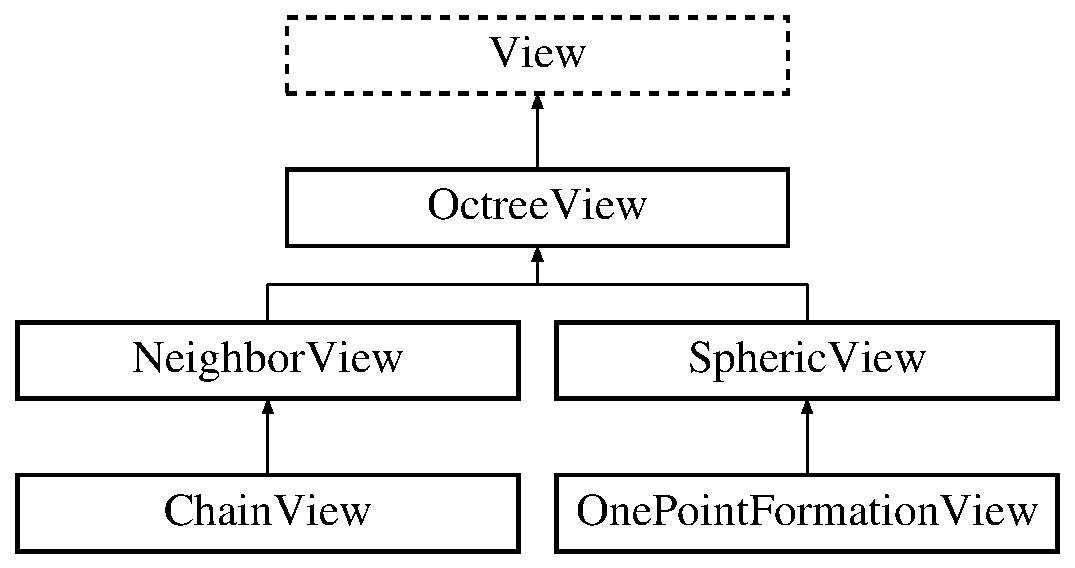
\includegraphics[height=4cm]{class_octree_view}
\end{center}
\end{figure}
\subsection*{Public Member Functions}
\begin{CompactItemize}
\item 
virtual void \hyperlink{class_octree_view_800b8d09dbd898769439f1765e7d87b1}{init} (const \hyperlink{class_world_information}{WorldInformation} \&world\_\-information)
\end{CompactItemize}
\subsection*{Protected Member Functions}
\begin{CompactItemize}
\item 
\hypertarget{class_octree_view_085a2326d14c933d278bce50391bde8a}{
const boost::shared\_\-ptr$<$ \hyperlink{class_octree}{Octree} $>$ \& \textbf{octree} () const }
\label{class_octree_view_085a2326d14c933d278bce50391bde8a}

\end{CompactItemize}
\subsection*{Protected Attributes}
\begin{CompactItemize}
\item 
\hypertarget{class_octree_view_2da509013a80d95319e5fc01d57d26c3}{
boost::shared\_\-ptr$<$ \hyperlink{class_octree}{Octree} $>$ \textbf{octree\_\-}}
\label{class_octree_view_2da509013a80d95319e5fc01d57d26c3}

\end{CompactItemize}


\subsection{Detailed Description}
\hyperlink{class_view}{View} sub class managing a octree. 

This class is designed as a base class for view sub classes needing an octree.

Abstract class, because it makes no sense to assign this class to a Robot since the view model provided by this class is the same as by \hyperlink{class_view}{View}. 

Definition at line 26 of file octree\_\-view.h.

\subsection{Member Function Documentation}
\hypertarget{class_octree_view_800b8d09dbd898769439f1765e7d87b1}{
\index{OctreeView@{OctreeView}!init@{init}}
\index{init@{init}!OctreeView@{OctreeView}}
\subsubsection[init]{\setlength{\rightskip}{0pt plus 5cm}void OctreeView::init (const {\bf WorldInformation} \& {\em world\_\-information})\hspace{0.3cm}{\tt  \mbox{[}virtual\mbox{]}}}}
\label{class_octree_view_800b8d09dbd898769439f1765e7d87b1}


Although init is trivial, it is nice to have a default constructor in virtual inherited classes. Otherwise every arbitrary deep sub class has to call the non-default constructor. Call this method before using any other method of \hyperlink{class_view}{View}. \begin{Desc}
\item[Parameters:]
\begin{description}
\item[{\em \hyperlink{class_world_information}{WorldInformation}}]\end{description}
\end{Desc}


Reimplemented from \hyperlink{class_view_fa489c0530d45e3e24c3151c0908240d}{View}.

Reimplemented in \hyperlink{class_spheric_view_dbd6a1d5e2f17594f82e831c38d35ec6}{SphericView}.

Definition at line 21 of file octree\_\-view.cc.

References View::init(), WorldInformation::markers(), WorldInformation::obstacles(), and WorldInformation::robot\_\-data().

The documentation for this class was generated from the following files:\begin{CompactItemize}
\item 
src/Views/octree\_\-view.h\item 
src/Views/octree\_\-view.cc\end{CompactItemize}

\hypertarget{class_one_point_formation_view}{
\section{OnePointFormationView Class Reference}
\label{class_one_point_formation_view}\index{OnePointFormationView@{OnePointFormationView}}
}
\hyperlink{class_view}{View} model of the 1PointFormation algorithm.  


{\tt \#include $<$one\_\-point\_\-formation\_\-view.h$>$}

Inheritance diagram for OnePointFormationView::\begin{figure}[H]
\begin{center}
\leavevmode
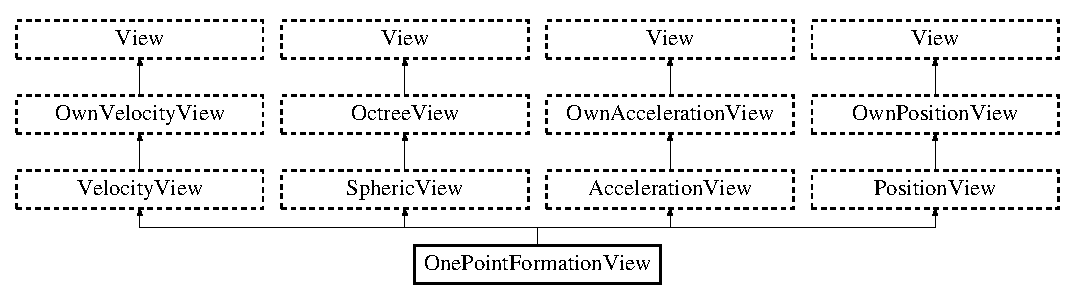
\includegraphics[height=3.58974cm]{class_one_point_formation_view}
\end{center}
\end{figure}
\subsection*{Public Member Functions}
\begin{CompactItemize}
\item 
\hypertarget{class_one_point_formation_view_4862bc6a8d1fc1e68e34e0be1f414e04}{
\textbf{OnePointFormationView} (double view\_\-radius)}
\label{class_one_point_formation_view_4862bc6a8d1fc1e68e34e0be1f414e04}

\end{CompactItemize}


\subsection{Detailed Description}
\hyperlink{class_view}{View} model of the 1PointFormation algorithm. 

Assigning this class to a Robot corresponds to the 1 Point Formation view model, i.e. every Robot can see every other Robots position, velocity and acceleration only in a limited radius. The coordinate-system and id of each Robot is not visible.

\begin{Desc}
\item[See also:]\href{https://wiki.math.uni-paderborn.de/pg-schwarm/StartSeite/AK/Szenarien}{\tt https://wiki.math.uni-paderborn.de/pg-schwarm/StartSeite/AK/Szenarien} \end{Desc}


Definition at line 27 of file one\_\-point\_\-formation\_\-view.h.

The documentation for this class was generated from the following files:\begin{CompactItemize}
\item 
src/Views/one\_\-point\_\-formation\_\-view.h\item 
src/Views/one\_\-point\_\-formation\_\-view.cc\end{CompactItemize}

\hypertarget{class_parametrized_view_factory}{
\section{ParametrizedViewFactory$<$ T, P $>$ Class Template Reference}
\label{class_parametrized_view_factory}\index{ParametrizedViewFactory@{ParametrizedViewFactory}}
}
{\tt \#include $<$parametrized\_\-view\_\-factory.h$>$}

Inheritance diagram for ParametrizedViewFactory$<$ T, P $>$::\begin{figure}[H]
\begin{center}
\leavevmode
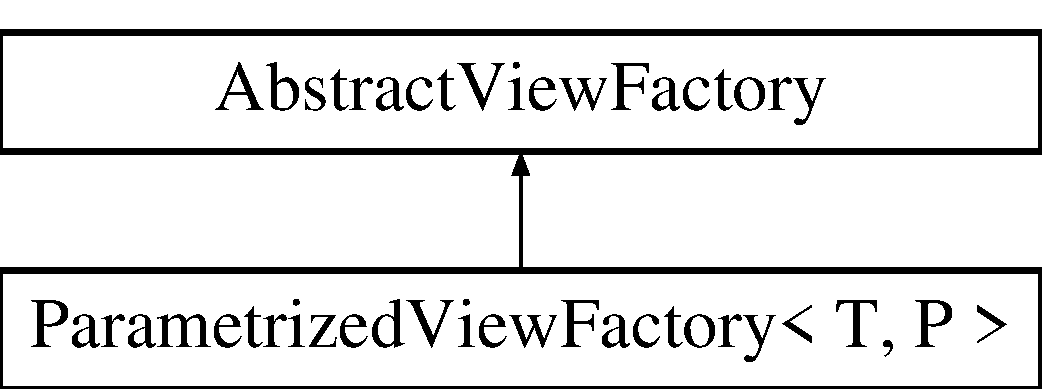
\includegraphics[height=2cm]{class_parametrized_view_factory}
\end{center}
\end{figure}
\subsection*{Public Member Functions}
\begin{CompactItemize}
\item 
\hypertarget{class_parametrized_view_factory_fb2dd21156ea282ac8bd5d008e2d7d55}{
\textbf{ParametrizedViewFactory} (const P \&argument)}
\label{class_parametrized_view_factory_fb2dd21156ea282ac8bd5d008e2d7d55}

\item 
\hypertarget{class_parametrized_view_factory_6ccbba555f6e406416113bd7c81ccab2}{
virtual boost::shared\_\-ptr$<$ \hyperlink{class_view}{View} $>$ \textbf{create\_\-new\_\-view\_\-instance} (const \hyperlink{class_world_information}{WorldInformation} \&world\_\-information) const }
\label{class_parametrized_view_factory_6ccbba555f6e406416113bd7c81ccab2}

\end{CompactItemize}
\subsection*{Private Attributes}
\begin{CompactItemize}
\item 
\hypertarget{class_parametrized_view_factory_1cccdef60401ee4afe6af7d9a15bc0ef}{
P \textbf{argument\_\-}}
\label{class_parametrized_view_factory_1cccdef60401ee4afe6af7d9a15bc0ef}

\end{CompactItemize}


\subsection{Detailed Description}
\subsubsection*{template$<$typename T, typename P$>$ class ParametrizedViewFactory$<$ T, P $>$}

Factory which can produce new \hyperlink{class_view}{View} objects. The type created is the template type of the factory. The second template type describes the parameter type of the \hyperlink{class_view}{View} constructor parameter. Constructor parameter determines the argument each created view class instance will get constructed with. 

Definition at line 23 of file parametrized\_\-view\_\-factory.h.

The documentation for this class was generated from the following file:\begin{CompactItemize}
\item 
src/Views/parametrized\_\-view\_\-factory.h\end{CompactItemize}

\hypertarget{class_position_request}{
\section{PositionRequest Class Reference}
\label{class_position_request}\index{PositionRequest@{PositionRequest}}
}
A position request is issued by a robot which wants to change its position to a new value.  


{\tt \#include $<$position\_\-request.h$>$}

Inheritance diagram for PositionRequest::\begin{figure}[H]
\begin{center}
\leavevmode
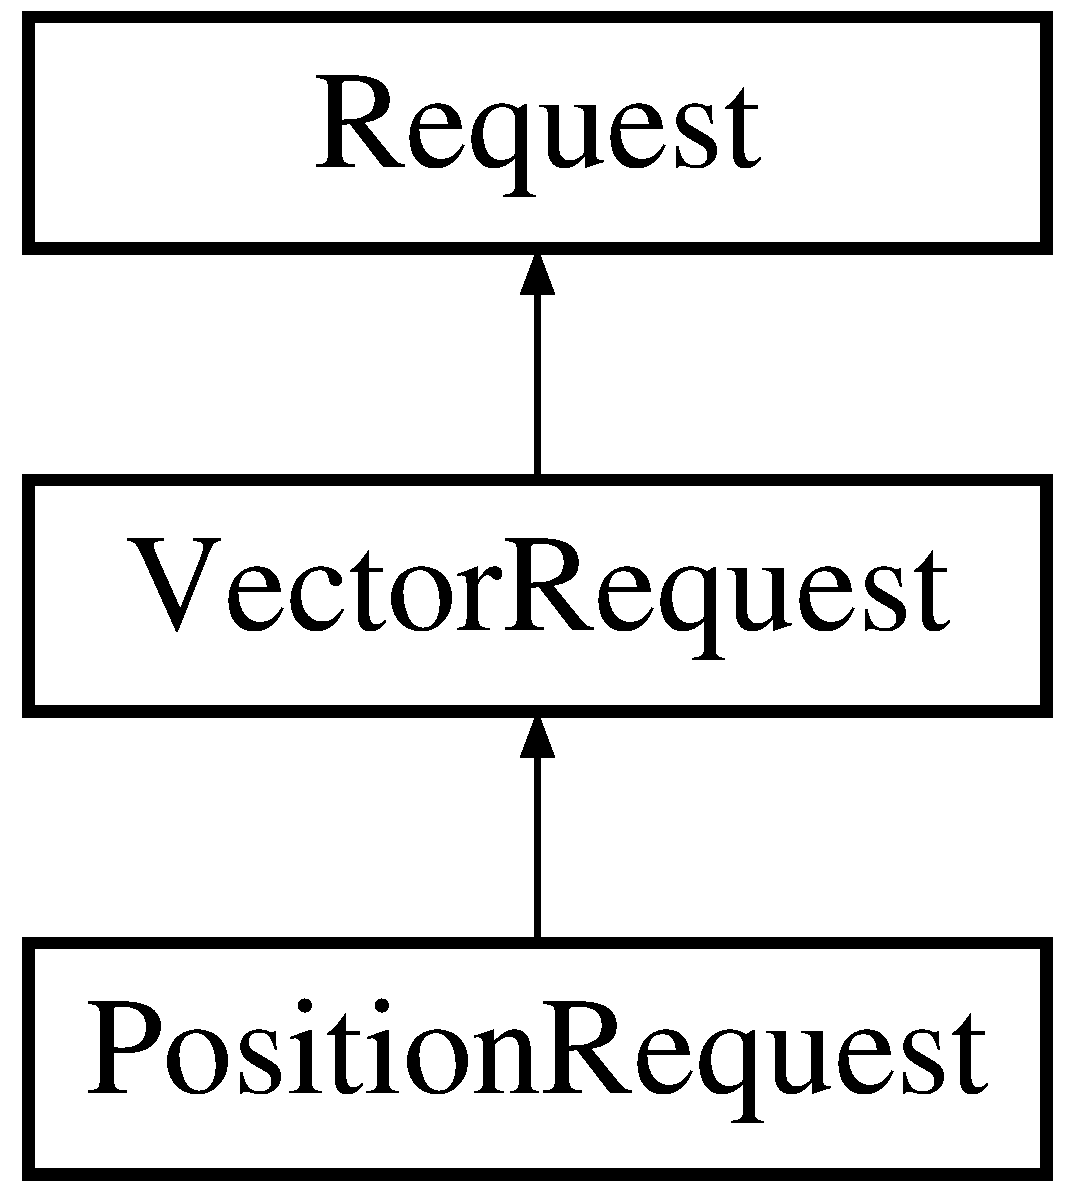
\includegraphics[height=3cm]{class_position_request}
\end{center}
\end{figure}
\subsection*{Public Member Functions}
\begin{CompactItemize}
\item 
\hypertarget{class_position_request_619ce34e18b2dcae4c36c59f59671719}{
\textbf{PositionRequest} (Robot \&robot, boost::shared\_\-ptr$<$ Vector3d $>$ requested\_\-vector)}
\label{class_position_request_619ce34e18b2dcae4c36c59f59671719}

\end{CompactItemize}


\subsection{Detailed Description}
A position request is issued by a robot which wants to change its position to a new value. 

Notes: The new position is expressed in terms of the local coordinate system of the robot. This means it has to be transformed before using.

The request cannot be changed after construction. 

Definition at line 23 of file position\_\-request.h.

The documentation for this class was generated from the following file:\begin{CompactItemize}
\item 
src/Requests/position\_\-request.h\end{CompactItemize}

\hypertarget{class_request}{
\section{Request Class Reference}
\label{class_request}\index{Request@{Request}}
}
Class which represents a request of a robot.  


{\tt \#include $<$request.h$>$}

Inheritance diagram for Request::\begin{figure}[H]
\begin{center}
\leavevmode
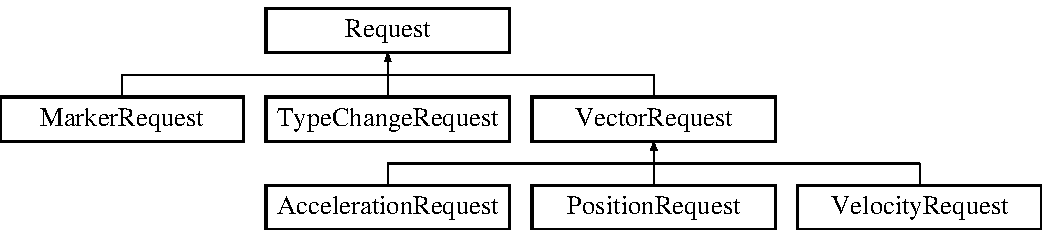
\includegraphics[height=3cm]{class_request}
\end{center}
\end{figure}
\subsection*{Public Member Functions}
\begin{CompactItemize}
\item 
\hypertarget{class_request_e6f2f79d4ba96802e0bc97bfe4d67c83}{
\textbf{Request} (Robot \&robot)}
\label{class_request_e6f2f79d4ba96802e0bc97bfe4d67c83}

\item 
const Robot \& \hyperlink{class_request_4bb10126bc0069cd7aa4dfe2f6d6c3fe}{robot} () const 
\end{CompactItemize}
\subsection*{Private Attributes}
\begin{CompactItemize}
\item 
Robot \& \hyperlink{class_request_2dcc3df8dd7a258caf4c605962581e8d}{robot\_\-}
\end{CompactItemize}


\subsection{Detailed Description}
Class which represents a request of a robot. 

Definition at line 19 of file request.h.

\subsection{Member Function Documentation}
\hypertarget{class_request_4bb10126bc0069cd7aa4dfe2f6d6c3fe}{
\index{Request@{Request}!robot@{robot}}
\index{robot@{robot}!Request@{Request}}
\subsubsection[robot]{\setlength{\rightskip}{0pt plus 5cm}const Robot\& Request::robot () const\hspace{0.3cm}{\tt  \mbox{[}inline\mbox{]}}}}
\label{class_request_4bb10126bc0069cd7aa4dfe2f6d6c3fe}


returns a constant reference to the robot which issued the request  a constant reference to the robot which issued the request 

Definition at line 28 of file request.h.

\subsection{Member Data Documentation}
\hypertarget{class_request_2dcc3df8dd7a258caf4c605962581e8d}{
\index{Request@{Request}!robot\_\-@{robot\_\-}}
\index{robot\_\-@{robot\_\-}!Request@{Request}}
\subsubsection[robot\_\-]{\setlength{\rightskip}{0pt plus 5cm}Robot\& {\bf Request::robot\_\-}\hspace{0.3cm}{\tt  \mbox{[}private\mbox{]}}}}
\label{class_request_2dcc3df8dd7a258caf4c605962581e8d}


The robot which issued the request. 

Definition at line 28 of file request.h.

The documentation for this class was generated from the following files:\begin{CompactItemize}
\item 
src/Requests/request.h\item 
src/Requests/request.cc\end{CompactItemize}

\hypertarget{class_request_handler}{
\section{RequestHandler Class Reference}
\label{class_request_handler}\index{RequestHandler@{RequestHandler}}
}
{\tt \#include $<$request\_\-handler.h$>$}

Inheritance diagram for RequestHandler::\begin{figure}[H]
\begin{center}
\leavevmode
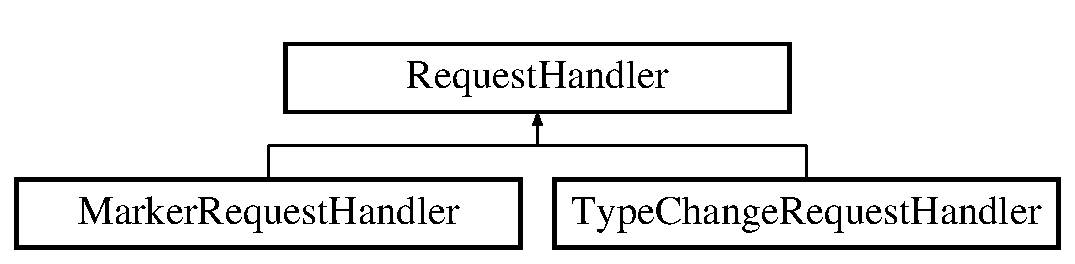
\includegraphics[height=2cm]{class_request_handler}
\end{center}
\end{figure}
\subsection*{Public Member Functions}
\begin{CompactItemize}
\item 
\hyperlink{class_request_handler_eb1589536489e52f0d6b0207f5d861d2}{RequestHandler} (unsigned int seed, double discard\_\-probability, const \hyperlink{class_history}{History} \&history)
\item 
void \hyperlink{class_request_handler_8f5f5cd120fdfa9774ea2e5f7886a908}{handle\_\-request} (boost::shared\_\-ptr$<$ \hyperlink{class_world_information}{WorldInformation} $>$ world\_\-information, boost::shared\_\-ptr$<$ const \hyperlink{class_request}{Request} $>$ request)
\end{CompactItemize}
\subsection*{Protected Attributes}
\begin{CompactItemize}
\item 
const \hyperlink{class_history}{History} \& \hyperlink{class_request_handler_a046537a35694efb8a288ed0b0283442}{history\_\-}
\end{CompactItemize}
\subsection*{Private Member Functions}
\begin{CompactItemize}
\item 
\hypertarget{class_request_handler_aee8881d705c6d20717e93d07a3929c4}{
virtual void \textbf{handle\_\-request\_\-reliable} (boost::shared\_\-ptr$<$ \hyperlink{class_world_information}{WorldInformation} $>$ world\_\-information, boost::shared\_\-ptr$<$ const \hyperlink{class_request}{Request} $>$ request)=0}
\label{class_request_handler_aee8881d705c6d20717e93d07a3929c4}

\end{CompactItemize}
\subsection*{Private Attributes}
\begin{CompactItemize}
\item 
\hypertarget{class_request_handler_adf54654024ab9b2aa41d50a69a2d8a8}{
double \textbf{discard\_\-probability\_\-}}
\label{class_request_handler_adf54654024ab9b2aa41d50a69a2d8a8}

\item 
\hypertarget{class_request_handler_045da9cac28878d81e8813d747a536d1}{
boost::shared\_\-ptr$<$ \hyperlink{class_distribution_generator}{DistributionGenerator} $>$ \textbf{distribution\_\-generator\_\-}}
\label{class_request_handler_045da9cac28878d81e8813d747a536d1}

\end{CompactItemize}


\subsection{Detailed Description}
abstract base class for handling requests. It implements unreliable handling of requests by randomly discarding them with the given discard probability. 

Definition at line 23 of file request\_\-handler.h.

\subsection{Constructor \& Destructor Documentation}
\hypertarget{class_request_handler_eb1589536489e52f0d6b0207f5d861d2}{
\index{RequestHandler@{RequestHandler}!RequestHandler@{RequestHandler}}
\index{RequestHandler@{RequestHandler}!RequestHandler@{RequestHandler}}
\subsubsection[RequestHandler]{\setlength{\rightskip}{0pt plus 5cm}RequestHandler::RequestHandler (unsigned int {\em seed}, \/  double {\em discard\_\-probability}, \/  const {\bf History} \& {\em history})}}
\label{class_request_handler_eb1589536489e52f0d6b0207f5d861d2}


constructs the \hyperlink{class_request_handler}{RequestHandler} by setting up the distribution generator with the given seed and discard probability. 

Definition at line 16 of file request\_\-handler.cc.

\subsection{Member Function Documentation}
\hypertarget{class_request_handler_8f5f5cd120fdfa9774ea2e5f7886a908}{
\index{RequestHandler@{RequestHandler}!handle\_\-request@{handle\_\-request}}
\index{handle\_\-request@{handle\_\-request}!RequestHandler@{RequestHandler}}
\subsubsection[handle\_\-request]{\setlength{\rightskip}{0pt plus 5cm}void RequestHandler::handle\_\-request (boost::shared\_\-ptr$<$ {\bf WorldInformation} $>$ {\em world\_\-information}, \/  boost::shared\_\-ptr$<$ const {\bf Request} $>$ {\em request})}}
\label{class_request_handler_8f5f5cd120fdfa9774ea2e5f7886a908}


discards the given request with the given probability. If not discarded the request is delegated to the abstract handle\_\-request\_\-reliable member.

Non-abstract RequestHandlers should implement handle\_\-request\_\-reliable 

Definition at line 26 of file request\_\-handler.cc.

\subsection{Member Data Documentation}
\hypertarget{class_request_handler_a046537a35694efb8a288ed0b0283442}{
\index{RequestHandler@{RequestHandler}!history\_\-@{history\_\-}}
\index{history\_\-@{history\_\-}!RequestHandler@{RequestHandler}}
\subsubsection[history\_\-]{\setlength{\rightskip}{0pt plus 5cm}const {\bf History}\& {\bf RequestHandler::history\_\-}\hspace{0.3cm}{\tt  \mbox{[}protected\mbox{]}}}}
\label{class_request_handler_a046537a35694efb8a288ed0b0283442}


\hyperlink{class_history}{History} may be used by inheriting classes to implement adversial behavior. 

Definition at line 45 of file request\_\-handler.h.

The documentation for this class was generated from the following files:\begin{CompactItemize}
\item 
src/EventHandlers/request\_\-handler.h\item 
src/EventHandlers/request\_\-handler.cc\end{CompactItemize}

\hypertarget{class_robot_control}{
\section{RobotControl Class Reference}
\label{class_robot_control}\index{RobotControl@{RobotControl}}
}
{\tt \#include $<$robot\_\-control.h$>$}

\subsection*{Public Member Functions}
\begin{CompactItemize}
\item 
\hyperlink{class_robot_control_2f44ebe0a98fff131117c10b3594381f}{RobotControl} (boost::shared\_\-ptr$<$ AbstractViewFactory $>$ view\_\-factory, std::size\_\-t history\_\-length, const \hyperlink{class_world_information}{WorldInformation} \&initial\_\-world\_\-information)
\item 
\hypertarget{class_robot_control_1d0bc5562cbfed424f029c09a38971ee}{
void \textbf{update} (const \hyperlink{class_world_information}{WorldInformation} \&world\_\-information)}
\label{class_robot_control_1d0bc5562cbfed424f029c09a38971ee}

\item 
std::set$<$ boost::shared\_\-ptr$<$ \hyperlink{class_request}{Request} $>$ $>$ \hyperlink{class_robot_control_55c97895d6d2a895ce67ecd118e7f1a0}{compute\_\-new\_\-request} (Robot \&robot)
\item 
void \hyperlink{class_robot_control_368f64b670eb9b3dd9488616832cafa9}{compute\_\-view} (Robot \&robot)
\item 
\hypertarget{class_robot_control_bca9b0186a6380e8838e47023a2626f9}{
void \textbf{set\_\-view\_\-facotry} (const boost::shared\_\-ptr$<$ AbstractViewFactory $>$ \&view\_\-factory)}
\label{class_robot_control_bca9b0186a6380e8838e47023a2626f9}

\end{CompactItemize}
\subsection*{Private Attributes}
\begin{CompactItemize}
\item 
\hypertarget{class_robot_control_928c58a2249ec85a6bbb742990db7551}{
boost::shared\_\-ptr$<$ AbstractViewFactory $>$ \textbf{view\_\-factory\_\-}}
\label{class_robot_control_928c58a2249ec85a6bbb742990db7551}

\item 
\hypertarget{class_robot_control_a6a8906b228423d0815d04a849e2e489}{
boost::circular\_\-buffer$<$ boost::shared\_\-ptr$<$ \hyperlink{class_view}{View} $>$ $>$ \textbf{view\_\-buffer\_\-}}
\label{class_robot_control_a6a8906b228423d0815d04a849e2e489}

\end{CompactItemize}


\subsection{Detailed Description}
Controls the Robots. Responsible for assigning the \hyperlink{class_view}{View} to each Robot and calling the compute method when requested.

\hyperlink{class_robot_control}{RobotControl} holds a buffer of Views of length history\_\-length. To do this, the \hyperlink{class_robot_control}{RobotControl} implements the \hyperlink{class_simulation_listener}{SimulationListener} interface. Whenever update is called together with an \hyperlink{class_handle_requests_event}{HandleRequestsEvent} \hyperlink{class_robot_control}{RobotControl} creates a new \hyperlink{class_view}{View} for the new WorldInfortion. 

Definition at line 36 of file robot\_\-control.h.

\subsection{Constructor \& Destructor Documentation}
\hypertarget{class_robot_control_2f44ebe0a98fff131117c10b3594381f}{
\index{RobotControl@{RobotControl}!RobotControl@{RobotControl}}
\index{RobotControl@{RobotControl}!RobotControl@{RobotControl}}
\subsubsection[RobotControl]{\setlength{\rightskip}{0pt plus 5cm}RobotControl::RobotControl (boost::shared\_\-ptr$<$ AbstractViewFactory $>$ {\em view\_\-factory}, \/  std::size\_\-t {\em history\_\-length}, \/  const {\bf WorldInformation} \& {\em initial\_\-world\_\-information})}}
\label{class_robot_control_2f44ebe0a98fff131117c10b3594381f}


Constructs a new \hyperlink{class_robot_control}{RobotControl}. \begin{Desc}
\item[Parameters:]
\begin{description}
\item[{\em The}]view\_\-factory given determines which view model should be used for the robots \item[{\em The}]length of the history \item[{\em intial}]\hyperlink{class_world_information}{WorldInformation} \end{description}
\end{Desc}
\begin{Desc}
\item[See also:]ModelParameters::HISTORY\_\-LENGTH \end{Desc}


Definition at line 13 of file robot\_\-control.cc.

\subsection{Member Function Documentation}
\hypertarget{class_robot_control_55c97895d6d2a895ce67ecd118e7f1a0}{
\index{RobotControl@{RobotControl}!compute\_\-new\_\-request@{compute\_\-new\_\-request}}
\index{compute\_\-new\_\-request@{compute\_\-new\_\-request}!RobotControl@{RobotControl}}
\subsubsection[compute\_\-new\_\-request]{\setlength{\rightskip}{0pt plus 5cm}std::set$<$ boost::shared\_\-ptr$<$ {\bf Request} $>$ $>$ RobotControl::compute\_\-new\_\-request (Robot \& {\em robot})}}
\label{class_robot_control_55c97895d6d2a895ce67ecd118e7f1a0}


Equivalent to robot.compute(). \begin{Desc}
\item[Parameters:]
\begin{description}
\item[{\em robot}]\item[{\em Set}]of Requests \end{description}
\end{Desc}
\begin{Desc}
\item[See also:]Robot::compute() \end{Desc}


Definition at line 28 of file robot\_\-control.cc.\hypertarget{class_robot_control_368f64b670eb9b3dd9488616832cafa9}{
\index{RobotControl@{RobotControl}!compute\_\-view@{compute\_\-view}}
\index{compute\_\-view@{compute\_\-view}!RobotControl@{RobotControl}}
\subsubsection[compute\_\-view]{\setlength{\rightskip}{0pt plus 5cm}void RobotControl::compute\_\-view (Robot \& {\em robot})}}
\label{class_robot_control_368f64b670eb9b3dd9488616832cafa9}


Computes and assigns the newest \hyperlink{class_view}{View} to the given robot. \begin{Desc}
\item[Parameters:]
\begin{description}
\item[{\em robot}]\end{description}
\end{Desc}


Definition at line 32 of file robot\_\-control.cc.

The documentation for this class was generated from the following files:\begin{CompactItemize}
\item 
src/SimulationKernel/robot\_\-control.h\item 
src/SimulationKernel/robot\_\-control.cc\end{CompactItemize}

\hypertarget{class_robot_data}{
\section{RobotData Class Reference}
\label{class_robot_data}\index{RobotData@{RobotData}}
}
Contains the properties a robot can have, but which are not necessarily visible to the robot and belong to the \hyperlink{class_world_information}{WorldInformation}.  


{\tt \#include $<$robot\_\-data.h$>$}

Inheritance diagram for RobotData::\begin{figure}[H]
\begin{center}
\leavevmode
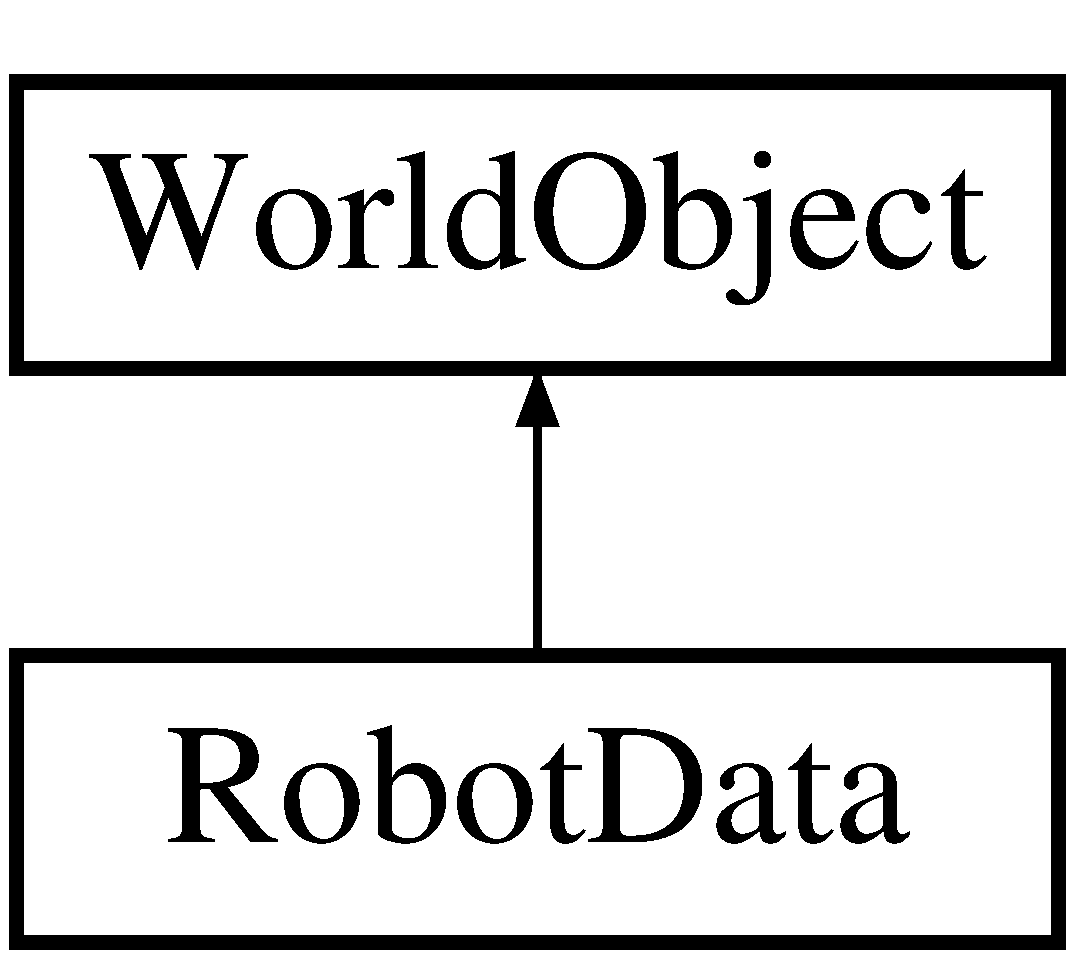
\includegraphics[height=2cm]{class_robot_data}
\end{center}
\end{figure}
\subsection*{Public Member Functions}
\begin{CompactItemize}
\item 
\hypertarget{class_robot_data_41a63a97d244ee80067af26873266d12}{
\textbf{RobotData} (boost::shared\_\-ptr$<$ \hyperlink{class_identifier}{Identifier} $>$ id, boost::shared\_\-ptr$<$ Vector3d $>$ position, const Robot \&robot)}
\label{class_robot_data_41a63a97d244ee80067af26873266d12}

\item 
\hypertarget{class_robot_data_11e1e006781a7bf7c26c93ef1ac04c21}{
\textbf{RobotData} (boost::shared\_\-ptr$<$ \hyperlink{class_identifier}{Identifier} $>$ id, boost::shared\_\-ptr$<$ Vector3d $>$ position, boost::shared\_\-ptr$<$ \hyperlink{class_marker_information}{MarkerInformation} $>$ marker\_\-information, const Robot \&robot)}
\label{class_robot_data_11e1e006781a7bf7c26c93ef1ac04c21}

\item 
\hypertarget{class_robot_data_23945633e0d7d4e732239c8f857dd2f1}{
\textbf{RobotData} (const \hyperlink{class_robot_data}{RobotData} \&rhs)}
\label{class_robot_data_23945633e0d7d4e732239c8f857dd2f1}

\item 
const Vector3d \& \hyperlink{class_robot_data_a65f6448e4ec4061b6300283f3cdd8da}{acceleration} () const 
\item 
void \hyperlink{class_robot_data_8799d69f51da76c16da773ca4cf8a8c5}{set\_\-acceleration} (boost::shared\_\-ptr$<$ Vector3d $>$ new\_\-acceleration)
\item 
const boost::tuple$<$ boost::shared\_\-ptr$<$ Vector3d $>$, boost::shared\_\-ptr$<$ Vector3d $>$, boost::shared\_\-ptr$<$ Vector3d $>$ $>$ \& \hyperlink{class_robot_data_e093fc063e47ad844c20a9332c5bea6a}{coordinate\_\-system\_\-axis} () const 
\item 
void \hyperlink{class_robot_data_26807404a2503711944c55f4ed75dd2e}{set\_\-coordinate\_\-system\_\-axis} (boost::tuple$<$ boost::shared\_\-ptr$<$ Vector3d $>$, boost::shared\_\-ptr$<$ Vector3d $>$, boost::shared\_\-ptr$<$ Vector3d $>$ $>$ new\_\-axes)
\item 
const RobotType \hyperlink{class_robot_data_b83255012ce788fdbf9b277c775e0240}{type} () const 
\item 
void \hyperlink{class_robot_data_ac8292bb51a92b2c5c9a6a6e00529fce}{set\_\-type} (RobotType type)
\item 
const Vector3d \& \hyperlink{class_robot_data_933da54224245d40afb0ed1b2446599c}{velocity} () const 
\item 
void \hyperlink{class_robot_data_4a45b387b65f7924015075bdcea2b00a}{set\_\-velocity} (boost::shared\_\-ptr$<$ Vector3d $>$ new\_\-velocity)
\item 
boost::shared\_\-ptr$<$ Vector3d $>$ \hyperlink{class_robot_data_5604cb6b35b70e6d70da6429349eec65}{extrapolated\_\-position} (double timesteps) const 
\item 
boost::shared\_\-ptr$<$ Vector3d $>$ \hyperlink{class_robot_data_37848feb0ad585292fd126465e126f67}{extrapolated\_\-velocity} (double timesteps) const 
\item 
RobotStatus \hyperlink{class_robot_data_9c8d2252555f1d5866c0332a80e82685}{status} () const 
\item 
void \hyperlink{class_robot_data_4a471efa8f681d3978f35f84caa77efd}{set\_\-status} (RobotStatus new\_\-status)
\item 
const Robot \& \hyperlink{class_robot_data_7e08f6f226617e6fda8f4b27e2622959}{robot} () const 
\item 
virtual boost::shared\_\-ptr$<$ \hyperlink{class_world_object}{WorldObject} $>$ \hyperlink{class_robot_data_81b5c3ba1f959f41ff3a9cb8067d75cb}{clone} () const 
\end{CompactItemize}
\subsection*{Private Attributes}
\begin{CompactItemize}
\item 
const Robot \& \hyperlink{class_robot_data_76bc912be93d4367f36234756b3bab7d}{robot\_\-}
\item 
\hypertarget{class_robot_data_da33b1d10cd1437104019459ca5cc214}{
boost::shared\_\-ptr$<$ Vector3d $>$ \textbf{acceleration\_\-}}
\label{class_robot_data_da33b1d10cd1437104019459ca5cc214}

\item 
\hypertarget{class_robot_data_5108482654c2bbfa3ff33e5be338ac2c}{
boost::tuple$<$ boost::shared\_\-ptr$<$ Vector3d $>$, boost::shared\_\-ptr$<$ Vector3d $>$, boost::shared\_\-ptr$<$ Vector3d $>$ $>$ \textbf{coordinate\_\-system\_\-axis\_\-}}
\label{class_robot_data_5108482654c2bbfa3ff33e5be338ac2c}

\item 
\hypertarget{class_robot_data_0ccbbf541e62a57ca12ffbb2239884c7}{
RobotType \textbf{type\_\-}}
\label{class_robot_data_0ccbbf541e62a57ca12ffbb2239884c7}

\item 
\hypertarget{class_robot_data_de8cc166cfa98dd9ef1ba1823111d82d}{
boost::shared\_\-ptr$<$ Vector3d $>$ \textbf{velocity\_\-}}
\label{class_robot_data_de8cc166cfa98dd9ef1ba1823111d82d}

\item 
\hypertarget{class_robot_data_8a991a0b98bdc099ab7e8c37394039a4}{
RobotStatus \textbf{status\_\-}}
\label{class_robot_data_8a991a0b98bdc099ab7e8c37394039a4}

\end{CompactItemize}


\subsection{Detailed Description}
Contains the properties a robot can have, but which are not necessarily visible to the robot and belong to the \hyperlink{class_world_information}{WorldInformation}. 

\begin{Desc}
\item[Author:]Martina Hüllmann \end{Desc}


Definition at line 34 of file robot\_\-data.h.

\subsection{Member Function Documentation}
\hypertarget{class_robot_data_a65f6448e4ec4061b6300283f3cdd8da}{
\index{RobotData@{RobotData}!acceleration@{acceleration}}
\index{acceleration@{acceleration}!RobotData@{RobotData}}
\subsubsection[acceleration]{\setlength{\rightskip}{0pt plus 5cm}const Vector3d \& RobotData::acceleration () const}}
\label{class_robot_data_a65f6448e4ec4061b6300283f3cdd8da}


Returns constant reference to acceleration vector of the robot. \begin{Desc}
\item[Returns:]Constant reference to acceleration vector of the robot. \end{Desc}


Definition at line 42 of file robot\_\-data.cc.

Referenced by extrapolated\_\-position(), and extrapolated\_\-velocity().\hypertarget{class_robot_data_8799d69f51da76c16da773ca4cf8a8c5}{
\index{RobotData@{RobotData}!set\_\-acceleration@{set\_\-acceleration}}
\index{set\_\-acceleration@{set\_\-acceleration}!RobotData@{RobotData}}
\subsubsection[set\_\-acceleration]{\setlength{\rightskip}{0pt plus 5cm}void RobotData::set\_\-acceleration (boost::shared\_\-ptr$<$ Vector3d $>$ {\em new\_\-acceleration})}}
\label{class_robot_data_8799d69f51da76c16da773ca4cf8a8c5}


Sets acceleration of the robot. \begin{Desc}
\item[Parameters:]
\begin{description}
\item[{\em Pointer}]to acceleration vector. \end{description}
\end{Desc}


Definition at line 46 of file robot\_\-data.cc.\hypertarget{class_robot_data_e093fc063e47ad844c20a9332c5bea6a}{
\index{RobotData@{RobotData}!coordinate\_\-system\_\-axis@{coordinate\_\-system\_\-axis}}
\index{coordinate\_\-system\_\-axis@{coordinate\_\-system\_\-axis}!RobotData@{RobotData}}
\subsubsection[coordinate\_\-system\_\-axis]{\setlength{\rightskip}{0pt plus 5cm}const boost::tuple$<$ boost::shared\_\-ptr$<$ Vector3d $>$, boost::shared\_\-ptr$<$ Vector3d $>$, boost::shared\_\-ptr$<$ Vector3d $>$ $>$ \& RobotData::coordinate\_\-system\_\-axis () const}}
\label{class_robot_data_e093fc063e47ad844c20a9332c5bea6a}


Returns constant reference to triple of pointers to vectors containing the coordinate system axis. \begin{Desc}
\item[Returns:]Triple of vectors containing the coordinate system axis. \end{Desc}


Definition at line 51 of file robot\_\-data.cc.\hypertarget{class_robot_data_26807404a2503711944c55f4ed75dd2e}{
\index{RobotData@{RobotData}!set\_\-coordinate\_\-system\_\-axis@{set\_\-coordinate\_\-system\_\-axis}}
\index{set\_\-coordinate\_\-system\_\-axis@{set\_\-coordinate\_\-system\_\-axis}!RobotData@{RobotData}}
\subsubsection[set\_\-coordinate\_\-system\_\-axis]{\setlength{\rightskip}{0pt plus 5cm}void RobotData::set\_\-coordinate\_\-system\_\-axis (boost::tuple$<$ boost::shared\_\-ptr$<$ Vector3d $>$, boost::shared\_\-ptr$<$ Vector3d $>$, boost::shared\_\-ptr$<$ Vector3d $>$ $>$ {\em new\_\-axes})}}
\label{class_robot_data_26807404a2503711944c55f4ed75dd2e}


Sets the coordinate system to the given triple of vectors. \begin{Desc}
\item[Parameters:]
\begin{description}
\item[{\em Triple}]of vectors for new axes. \end{description}
\end{Desc}


Definition at line 55 of file robot\_\-data.cc.\hypertarget{class_robot_data_b83255012ce788fdbf9b277c775e0240}{
\index{RobotData@{RobotData}!type@{type}}
\index{type@{type}!RobotData@{RobotData}}
\subsubsection[type]{\setlength{\rightskip}{0pt plus 5cm}const RobotType RobotData::type () const}}
\label{class_robot_data_b83255012ce788fdbf9b277c775e0240}


Returns type of the robot. \begin{Desc}
\item[Returns:]type of the robot. \end{Desc}


Definition at line 60 of file robot\_\-data.cc.\hypertarget{class_robot_data_ac8292bb51a92b2c5c9a6a6e00529fce}{
\index{RobotData@{RobotData}!set\_\-type@{set\_\-type}}
\index{set\_\-type@{set\_\-type}!RobotData@{RobotData}}
\subsubsection[set\_\-type]{\setlength{\rightskip}{0pt plus 5cm}void RobotData::set\_\-type (RobotType {\em type})\hspace{0.3cm}{\tt  \mbox{[}inline\mbox{]}}}}
\label{class_robot_data_ac8292bb51a92b2c5c9a6a6e00529fce}


Sets the type of the robot. \begin{Desc}
\item[Parameters:]
\begin{description}
\item[{\em new}]type \end{description}
\end{Desc}


Definition at line 83 of file robot\_\-data.h.\hypertarget{class_robot_data_933da54224245d40afb0ed1b2446599c}{
\index{RobotData@{RobotData}!velocity@{velocity}}
\index{velocity@{velocity}!RobotData@{RobotData}}
\subsubsection[velocity]{\setlength{\rightskip}{0pt plus 5cm}const Vector3d \& RobotData::velocity () const}}
\label{class_robot_data_933da54224245d40afb0ed1b2446599c}


Returns constant reference to velocity vector of the robot. \begin{Desc}
\item[Returns:]constant reference Velocity vector of the robot. \end{Desc}


Definition at line 64 of file robot\_\-data.cc.

Referenced by extrapolated\_\-position(), and extrapolated\_\-velocity().\hypertarget{class_robot_data_4a45b387b65f7924015075bdcea2b00a}{
\index{RobotData@{RobotData}!set\_\-velocity@{set\_\-velocity}}
\index{set\_\-velocity@{set\_\-velocity}!RobotData@{RobotData}}
\subsubsection[set\_\-velocity]{\setlength{\rightskip}{0pt plus 5cm}void RobotData::set\_\-velocity (boost::shared\_\-ptr$<$ Vector3d $>$ {\em new\_\-velocity})}}
\label{class_robot_data_4a45b387b65f7924015075bdcea2b00a}


Sets velocity of the robot. \begin{Desc}
\item[Parameters:]
\begin{description}
\item[{\em Pointer}]to new velocity vector. \end{description}
\end{Desc}


Definition at line 68 of file robot\_\-data.cc.\hypertarget{class_robot_data_5604cb6b35b70e6d70da6429349eec65}{
\index{RobotData@{RobotData}!extrapolated\_\-position@{extrapolated\_\-position}}
\index{extrapolated\_\-position@{extrapolated\_\-position}!RobotData@{RobotData}}
\subsubsection[extrapolated\_\-position]{\setlength{\rightskip}{0pt plus 5cm}boost::shared\_\-ptr$<$ Vector3d $>$ RobotData::extrapolated\_\-position (double {\em timesteps}) const}}
\label{class_robot_data_5604cb6b35b70e6d70da6429349eec65}


Returns position of the robot at the moment some timesteps in the future. \begin{Desc}
\item[Parameters:]
\begin{description}
\item[{\em double}]for additional timesteps \end{description}
\end{Desc}
\begin{Desc}
\item[Returns:]Vector3d for coordinates \end{Desc}


Definition at line 72 of file robot\_\-data.cc.

References acceleration(), WorldObject::position(), and velocity().\hypertarget{class_robot_data_37848feb0ad585292fd126465e126f67}{
\index{RobotData@{RobotData}!extrapolated\_\-velocity@{extrapolated\_\-velocity}}
\index{extrapolated\_\-velocity@{extrapolated\_\-velocity}!RobotData@{RobotData}}
\subsubsection[extrapolated\_\-velocity]{\setlength{\rightskip}{0pt plus 5cm}boost::shared\_\-ptr$<$ Vector3d $>$ RobotData::extrapolated\_\-velocity (double {\em timesteps}) const}}
\label{class_robot_data_37848feb0ad585292fd126465e126f67}


Returns velocity of the robot at the moment some timesteps in the future. \begin{Desc}
\item[Parameters:]
\begin{description}
\item[{\em double}]for additional timesteps \end{description}
\end{Desc}
\begin{Desc}
\item[Returns:]Vector3d for coordinates \end{Desc}


Definition at line 84 of file robot\_\-data.cc.

References acceleration(), and velocity().\hypertarget{class_robot_data_9c8d2252555f1d5866c0332a80e82685}{
\index{RobotData@{RobotData}!status@{status}}
\index{status@{status}!RobotData@{RobotData}}
\subsubsection[status]{\setlength{\rightskip}{0pt plus 5cm}RobotStatus RobotData::status () const}}
\label{class_robot_data_9c8d2252555f1d5866c0332a80e82685}


Returns status of the robot. \begin{Desc}
\item[Returns:]Status of the robot. \end{Desc}


Definition at line 92 of file robot\_\-data.cc.\hypertarget{class_robot_data_4a471efa8f681d3978f35f84caa77efd}{
\index{RobotData@{RobotData}!set\_\-status@{set\_\-status}}
\index{set\_\-status@{set\_\-status}!RobotData@{RobotData}}
\subsubsection[set\_\-status]{\setlength{\rightskip}{0pt plus 5cm}void RobotData::set\_\-status (RobotStatus {\em new\_\-status})}}
\label{class_robot_data_4a471efa8f681d3978f35f84caa77efd}


Sets status of the robot. \begin{Desc}
\item[Parameters:]
\begin{description}
\item[{\em new}]status \end{description}
\end{Desc}


Definition at line 96 of file robot\_\-data.cc.\hypertarget{class_robot_data_7e08f6f226617e6fda8f4b27e2622959}{
\index{RobotData@{RobotData}!robot@{robot}}
\index{robot@{robot}!RobotData@{RobotData}}
\subsubsection[robot]{\setlength{\rightskip}{0pt plus 5cm}const Robot \& RobotData::robot () const}}
\label{class_robot_data_7e08f6f226617e6fda8f4b27e2622959}


Returns reference to according robot-object. \begin{Desc}
\item[Returns:]Reference to according robot-object. \end{Desc}


Definition at line 100 of file robot\_\-data.cc.

References robot\_\-.\hypertarget{class_robot_data_81b5c3ba1f959f41ff3a9cb8067d75cb}{
\index{RobotData@{RobotData}!clone@{clone}}
\index{clone@{clone}!RobotData@{RobotData}}
\subsubsection[clone]{\setlength{\rightskip}{0pt plus 5cm}boost::shared\_\-ptr$<$ {\bf WorldObject} $>$ RobotData::clone () const\hspace{0.3cm}{\tt  \mbox{[}virtual\mbox{]}}}}
\label{class_robot_data_81b5c3ba1f959f41ff3a9cb8067d75cb}


Clones this object and returns a shared ptr to the cloned object. typeid($\ast$this) == typeid($\ast$clone) \begin{Desc}
\item[Returns:]shared ptr to the cloned object \end{Desc}


Reimplemented from \hyperlink{class_world_object_dba468299ce77ce5781e60081bf44b14}{WorldObject}.

Definition at line 104 of file robot\_\-data.cc.

\subsection{Member Data Documentation}
\hypertarget{class_robot_data_76bc912be93d4367f36234756b3bab7d}{
\index{RobotData@{RobotData}!robot\_\-@{robot\_\-}}
\index{robot\_\-@{robot\_\-}!RobotData@{RobotData}}
\subsubsection[robot\_\-]{\setlength{\rightskip}{0pt plus 5cm}const Robot\& {\bf RobotData::robot\_\-}\hspace{0.3cm}{\tt  \mbox{[}private\mbox{]}}}}
\label{class_robot_data_76bc912be93d4367f36234756b3bab7d}


Reference to according robot. 

Definition at line 134 of file robot\_\-data.h.

Referenced by robot().

The documentation for this class was generated from the following files:\begin{CompactItemize}
\item 
src/Model/robot\_\-data.h\item 
src/Model/robot\_\-data.cc\end{CompactItemize}

\hypertarget{class_robot_identifier}{
\section{RobotIdentifier Class Reference}
\label{class_robot_identifier}\index{RobotIdentifier@{RobotIdentifier}}
}
Denote ID's of robots.  


{\tt \#include $<$robot\_\-identifier.h$>$}

Inheritance diagram for RobotIdentifier::\begin{figure}[H]
\begin{center}
\leavevmode
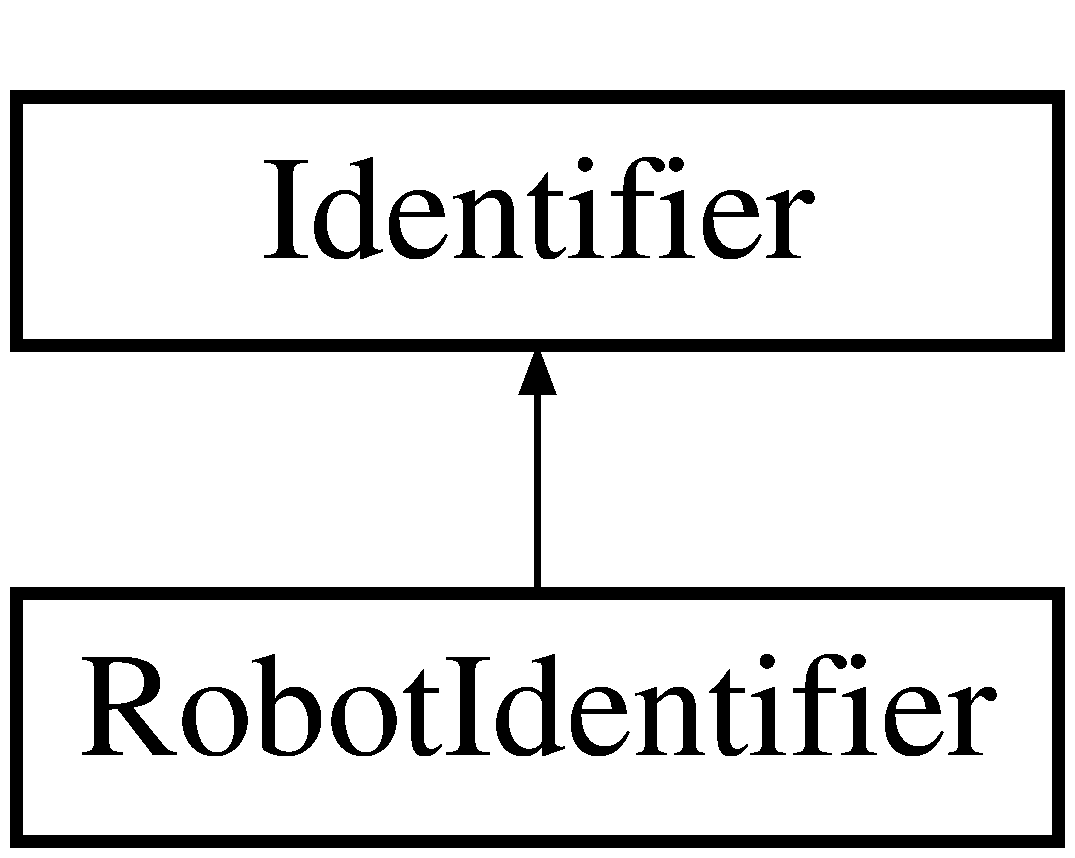
\includegraphics[height=2cm]{class_robot_identifier}
\end{center}
\end{figure}
\subsection*{Public Member Functions}
\begin{CompactItemize}
\item 
\hypertarget{class_robot_identifier_06b6379fa91d4d7ae0b74ff734c0bd69}{
\textbf{RobotIdentifier} (std::size\_\-t id)}
\label{class_robot_identifier_06b6379fa91d4d7ae0b74ff734c0bd69}

\item 
\hypertarget{class_robot_identifier_940b1d28c51fe39e360c34ebaac9a7ad}{
virtual boost::shared\_\-ptr$<$ \hyperlink{class_identifier}{Identifier} $>$ \textbf{clone} () const }
\label{class_robot_identifier_940b1d28c51fe39e360c34ebaac9a7ad}

\end{CompactItemize}


\subsection{Detailed Description}
Denote ID's of robots. 

\begin{Desc}
\item[Author:]Martina Hüllmann \end{Desc}


Definition at line 15 of file robot\_\-identifier.h.

The documentation for this class was generated from the following files:\begin{CompactItemize}
\item 
src/Model/robot\_\-identifier.h\item 
src/Model/robot\_\-identifier.cc\end{CompactItemize}

\hypertarget{class_self_view}{
\section{SelfView Class Reference}
\label{class_self_view}\index{SelfView@{SelfView}}
}
\char`\"{}Known everything about yourself, but nothing about others\char`\"{} view model.  


{\tt \#include $<$self\_\-view.h$>$}

Inheritance diagram for SelfView::\begin{figure}[H]
\begin{center}
\leavevmode
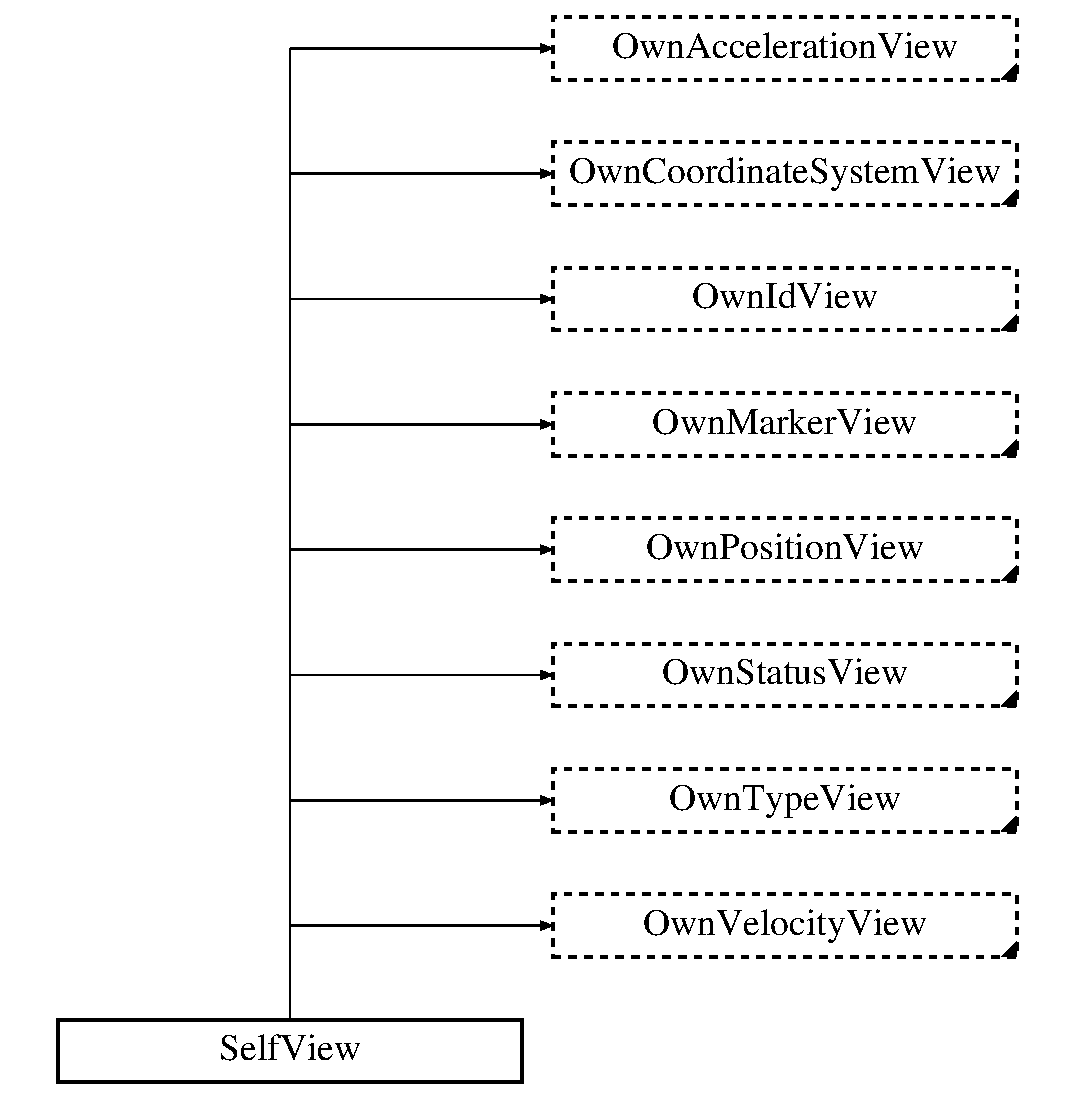
\includegraphics[height=9cm]{class_self_view}
\end{center}
\end{figure}


\subsection{Detailed Description}
\char`\"{}Known everything about yourself, but nothing about others\char`\"{} view model. 

Assigning this class to a Robot corresponds to a \char`\"{}known everything about yourself, but nothing about others\char`\"{} model. 

Definition at line 28 of file self\_\-view.h.

The documentation for this class was generated from the following files:\begin{CompactItemize}
\item 
src/Views/self\_\-view.h\item 
src/Views/self\_\-view.cc\end{CompactItemize}

\hypertarget{class_simulation_control}{
\section{SimulationControl Class Reference}
\label{class_simulation_control}\index{SimulationControl@{SimulationControl}}
}
Controls the simulation.  


{\tt \#include $<$simulation\_\-control.h$>$}

Inherited by SampleControl.

\subsection*{Public Member Functions}
\begin{CompactItemize}
\item 
void \hyperlink{class_simulation_control_4571c7dae922020316b8f2069a6297a2}{create\_\-new\_\-simulation} (const std::string \&configuration\_\-filename, std::size\_\-t history\_\-length)
\item 
void \hyperlink{class_simulation_control_cf99b31b2a40f9162445b4e06095dda2}{start\_\-simulation} ()
\item 
void \hyperlink{class_simulation_control_edae523153b33eea2bb79c0f7b3076f1}{pause\_\-simulation} ()
\item 
void \hyperlink{class_simulation_control_8e9cd7b65a4757d3af067a459144a94c}{terminate\_\-simulation} ()
\item 
void \hyperlink{class_simulation_control_c22664bf7cf9fd4280787123b01a970e}{process\_\-simulation} ()
\item 
void \hyperlink{class_simulation_control_2e3eb01723381bbaaa80f4700e4aba4e}{set\_\-visualizer} (boost::shared\_\-ptr$<$ Visualizer $>$ visualizer)
\end{CompactItemize}
\subsection*{Private Member Functions}
\begin{CompactItemize}
\item 
\hypertarget{class_simulation_control_44d5e77f43e0b3cd5e008bc63c19f65d}{
double \textbf{compute\_\-new\_\-processing\_\-time} ()}
\label{class_simulation_control_44d5e77f43e0b3cd5e008bc63c19f65d}

\end{CompactItemize}
\subsection*{Private Attributes}
\begin{CompactItemize}
\item 
\hypertarget{class_simulation_control_0435ad5ef168d1952c733ae05ce06784}{
double \textbf{processing\_\-time\_\-factor\_\-}}
\label{class_simulation_control_0435ad5ef168d1952c733ae05ce06784}

\item 
\hypertarget{class_simulation_control_ce445691937d7972b7fd19e590b5279e}{
double \textbf{current\_\-processing\_\-time\_\-}}
\label{class_simulation_control_ce445691937d7972b7fd19e590b5279e}

\item 
\hypertarget{class_simulation_control_34faee52b56375399307ec229bdbd412}{
boost::posix\_\-time::ptime \textbf{last\_\-process\_\-simulation\_\-time\_\-}}
\label{class_simulation_control_34faee52b56375399307ec229bdbd412}

\item 
\hypertarget{class_simulation_control_a22c3ae0c981bd7cc956a7189606d3df}{
boost::shared\_\-ptr$<$ \hyperlink{class_world_information}{WorldInformation} $>$ \textbf{current\_\-world\_\-information\_\-}}
\label{class_simulation_control_a22c3ae0c981bd7cc956a7189606d3df}

\item 
\hypertarget{class_simulation_control_ab2be5f82be231fc495ef504df050a15}{
boost::shared\_\-ptr$<$ \hyperlink{class_world_information}{WorldInformation} $>$ \textbf{next\_\-world\_\-information\_\-}}
\label{class_simulation_control_ab2be5f82be231fc495ef504df050a15}

\item 
\hypertarget{class_simulation_control_69e51cca0a4925987cba9b00aa604290}{
boost::shared\_\-ptr$<$ \hyperlink{class_history}{History} $>$ \textbf{history\_\-}}
\label{class_simulation_control_69e51cca0a4925987cba9b00aa604290}

\item 
\hypertarget{class_simulation_control_3bad0ca00bcec0a1580cccde6545114a}{
boost::shared\_\-ptr$<$ \hyperlink{class_simulation_control_1_1_simulation_kernel_functor}{SimulationKernelFunctor} $>$ \textbf{simulation\_\-kernel\_\-functor\_\-}}
\label{class_simulation_control_3bad0ca00bcec0a1580cccde6545114a}

\item 
\hypertarget{class_simulation_control_54cbf830e33518eea2c1305921f46657}{
boost::thread \textbf{simulation\_\-thread\_\-}}
\label{class_simulation_control_54cbf830e33518eea2c1305921f46657}

\item 
\hypertarget{class_simulation_control_e0921fe6a32e848db09a3bf5d53dbc37}{
boost::shared\_\-ptr$<$ Visualizer $>$ \textbf{visualizer\_\-}}
\label{class_simulation_control_e0921fe6a32e848db09a3bf5d53dbc37}

\end{CompactItemize}
\subsection*{Classes}
\begin{CompactItemize}
\item 
class \hyperlink{class_simulation_control_1_1_simulation_kernel_functor}{SimulationKernelFunctor}
\end{CompactItemize}


\subsection{Detailed Description}
Controls the simulation. 

The class \hyperlink{class_simulation_control}{SimulationControl} provides code to set up a new simulation (and cleanup any old one) as well as start/pause/terminate the Simulation�Thread. Furthermore it provides a method called process simulation that is responsible for consuming the history�s elements according to the Processing�Time.

\begin{Desc}
\item[Author:]Daniel Wonisch \end{Desc}


Definition at line 30 of file simulation\_\-control.h.

\subsection{Member Function Documentation}
\hypertarget{class_simulation_control_4571c7dae922020316b8f2069a6297a2}{
\index{SimulationControl@{SimulationControl}!create\_\-new\_\-simulation@{create\_\-new\_\-simulation}}
\index{create\_\-new\_\-simulation@{create\_\-new\_\-simulation}!SimulationControl@{SimulationControl}}
\subsubsection[create\_\-new\_\-simulation]{\setlength{\rightskip}{0pt plus 5cm}void SimulationControl::create\_\-new\_\-simulation (const std::string \& {\em configuration\_\-filename}, \/  std::size\_\-t {\em history\_\-length})}}
\label{class_simulation_control_4571c7dae922020316b8f2069a6297a2}


cleans up the old simulation and creates a new one without starting it. 

Definition at line 24 of file simulation\_\-control.cc.

References terminate\_\-simulation().\hypertarget{class_simulation_control_cf99b31b2a40f9162445b4e06095dda2}{
\index{SimulationControl@{SimulationControl}!start\_\-simulation@{start\_\-simulation}}
\index{start\_\-simulation@{start\_\-simulation}!SimulationControl@{SimulationControl}}
\subsubsection[start\_\-simulation]{\setlength{\rightskip}{0pt plus 5cm}void SimulationControl::start\_\-simulation ()}}
\label{class_simulation_control_cf99b31b2a40f9162445b4e06095dda2}


starts the simulation 

Definition at line 51 of file simulation\_\-control.cc.

References SimulationControl::SimulationKernelFunctor::loop().\hypertarget{class_simulation_control_edae523153b33eea2bb79c0f7b3076f1}{
\index{SimulationControl@{SimulationControl}!pause\_\-simulation@{pause\_\-simulation}}
\index{pause\_\-simulation@{pause\_\-simulation}!SimulationControl@{SimulationControl}}
\subsubsection[pause\_\-simulation]{\setlength{\rightskip}{0pt plus 5cm}void SimulationControl::pause\_\-simulation ()}}
\label{class_simulation_control_edae523153b33eea2bb79c0f7b3076f1}


pauses the simulation 

Definition at line 69 of file simulation\_\-control.cc.\hypertarget{class_simulation_control_8e9cd7b65a4757d3af067a459144a94c}{
\index{SimulationControl@{SimulationControl}!terminate\_\-simulation@{terminate\_\-simulation}}
\index{terminate\_\-simulation@{terminate\_\-simulation}!SimulationControl@{SimulationControl}}
\subsubsection[terminate\_\-simulation]{\setlength{\rightskip}{0pt plus 5cm}void SimulationControl::terminate\_\-simulation ()}}
\label{class_simulation_control_8e9cd7b65a4757d3af067a459144a94c}


terminates simulation and cleans up the simulation thread 

Definition at line 75 of file simulation\_\-control.cc.

Referenced by create\_\-new\_\-simulation().\hypertarget{class_simulation_control_c22664bf7cf9fd4280787123b01a970e}{
\index{SimulationControl@{SimulationControl}!process\_\-simulation@{process\_\-simulation}}
\index{process\_\-simulation@{process\_\-simulation}!SimulationControl@{SimulationControl}}
\subsubsection[process\_\-simulation]{\setlength{\rightskip}{0pt plus 5cm}void SimulationControl::process\_\-simulation ()}}
\label{class_simulation_control_c22664bf7cf9fd4280787123b01a970e}


process the simulation: advances the processing time and calls the visualizer if there is one. 

Definition at line 86 of file simulation\_\-control.cc.\hypertarget{class_simulation_control_2e3eb01723381bbaaa80f4700e4aba4e}{
\index{SimulationControl@{SimulationControl}!set\_\-visualizer@{set\_\-visualizer}}
\index{set\_\-visualizer@{set\_\-visualizer}!SimulationControl@{SimulationControl}}
\subsubsection[set\_\-visualizer]{\setlength{\rightskip}{0pt plus 5cm}void SimulationControl::set\_\-visualizer (boost::shared\_\-ptr$<$ Visualizer $>$ {\em visualizer})}}
\label{class_simulation_control_2e3eb01723381bbaaa80f4700e4aba4e}


supplies the control with a new visualizer. 

The documentation for this class was generated from the following files:\begin{CompactItemize}
\item 
src/SimulationControl/simulation\_\-control.h\item 
src/SimulationControl/simulation\_\-control.cc\end{CompactItemize}

\hypertarget{class_simulation_control_1_1_simulation_kernel_functor}{
\section{SimulationControl::SimulationKernelFunctor Class Reference}
\label{class_simulation_control_1_1_simulation_kernel_functor}\index{SimulationControl::SimulationKernelFunctor@{SimulationControl::SimulationKernelFunctor}}
}
\subsection*{Public Member Functions}
\begin{CompactItemize}
\item 
\hyperlink{class_simulation_control_1_1_simulation_kernel_functor_5264e83328beeaafae7e87179614c436}{SimulationKernelFunctor} (boost::shared\_\-ptr$<$ \hyperlink{class_simulation_kernel}{SimulationKernel} $>$ simulation\_\-kernel)
\item 
void \hyperlink{class_simulation_control_1_1_simulation_kernel_functor_c23f51cedb9c10e346a7bb6a66ed98ab}{unpause} ()
\item 
void \hyperlink{class_simulation_control_1_1_simulation_kernel_functor_1228e457d2a780ba379b36e66f57e8cd}{pause} ()
\item 
void \hyperlink{class_simulation_control_1_1_simulation_kernel_functor_afb53670154b6460d79358f9b866ef24}{terminate} ()
\item 
void \hyperlink{class_simulation_control_1_1_simulation_kernel_functor_44aaca5c7b6605436b889d41cc4b9472}{loop} ()
\end{CompactItemize}
\subsection*{Private Attributes}
\begin{CompactItemize}
\item 
bool \hyperlink{class_simulation_control_1_1_simulation_kernel_functor_0803093cc15c83a7b85044ae2d630270}{terminated\_\-}
\item 
bool \hyperlink{class_simulation_control_1_1_simulation_kernel_functor_c0b1b92a6a04db5775afbcbae5a734ec}{paused\_\-}
\item 
\hypertarget{class_simulation_control_1_1_simulation_kernel_functor_d513c7e18afaed223c9477654d33638e}{
boost::interprocess::interprocess\_\-semaphore \textbf{unpaused\_\-}}
\label{class_simulation_control_1_1_simulation_kernel_functor_d513c7e18afaed223c9477654d33638e}

\item 
\hypertarget{class_simulation_control_1_1_simulation_kernel_functor_ee9b24898cfae41f76f8fd096cdcab24}{
boost::shared\_\-ptr$<$ \hyperlink{class_simulation_kernel}{SimulationKernel} $>$ \textbf{simulation\_\-kernel\_\-}}
\label{class_simulation_control_1_1_simulation_kernel_functor_ee9b24898cfae41f76f8fd096cdcab24}

\end{CompactItemize}


\subsection{Detailed Description}
Thread-Wrapper for the simulation kernel. Allows the simulation kernel thread to be paused and unpaused. 

Definition at line 70 of file simulation\_\-control.h.

\subsection{Constructor \& Destructor Documentation}
\hypertarget{class_simulation_control_1_1_simulation_kernel_functor_5264e83328beeaafae7e87179614c436}{
\index{SimulationControl::SimulationKernelFunctor@{SimulationControl::SimulationKernelFunctor}!SimulationKernelFunctor@{SimulationKernelFunctor}}
\index{SimulationKernelFunctor@{SimulationKernelFunctor}!SimulationControl::SimulationKernelFunctor@{SimulationControl::SimulationKernelFunctor}}
\subsubsection[SimulationKernelFunctor]{\setlength{\rightskip}{0pt plus 5cm}SimulationControl::SimulationKernelFunctor::SimulationKernelFunctor (boost::shared\_\-ptr$<$ {\bf SimulationKernel} $>$ {\em simulation\_\-kernel})}}
\label{class_simulation_control_1_1_simulation_kernel_functor_5264e83328beeaafae7e87179614c436}


constructs a new functor with the given simulation kernel thread. 

Definition at line 127 of file simulation\_\-control.cc.

\subsection{Member Function Documentation}
\hypertarget{class_simulation_control_1_1_simulation_kernel_functor_c23f51cedb9c10e346a7bb6a66ed98ab}{
\index{SimulationControl::SimulationKernelFunctor@{SimulationControl::SimulationKernelFunctor}!unpause@{unpause}}
\index{unpause@{unpause}!SimulationControl::SimulationKernelFunctor@{SimulationControl::SimulationKernelFunctor}}
\subsubsection[unpause]{\setlength{\rightskip}{0pt plus 5cm}void SimulationControl::SimulationKernelFunctor::unpause ()}}
\label{class_simulation_control_1_1_simulation_kernel_functor_c23f51cedb9c10e346a7bb6a66ed98ab}


unpauses the simulation thread using a semaphor 

Definition at line 132 of file simulation\_\-control.cc.

References paused\_\-.\hypertarget{class_simulation_control_1_1_simulation_kernel_functor_1228e457d2a780ba379b36e66f57e8cd}{
\index{SimulationControl::SimulationKernelFunctor@{SimulationControl::SimulationKernelFunctor}!pause@{pause}}
\index{pause@{pause}!SimulationControl::SimulationKernelFunctor@{SimulationControl::SimulationKernelFunctor}}
\subsubsection[pause]{\setlength{\rightskip}{0pt plus 5cm}void SimulationControl::SimulationKernelFunctor::pause ()}}
\label{class_simulation_control_1_1_simulation_kernel_functor_1228e457d2a780ba379b36e66f57e8cd}


pauses the simulation thread using a semaphor 

Definition at line 140 of file simulation\_\-control.cc.

References paused\_\-.\hypertarget{class_simulation_control_1_1_simulation_kernel_functor_afb53670154b6460d79358f9b866ef24}{
\index{SimulationControl::SimulationKernelFunctor@{SimulationControl::SimulationKernelFunctor}!terminate@{terminate}}
\index{terminate@{terminate}!SimulationControl::SimulationKernelFunctor@{SimulationControl::SimulationKernelFunctor}}
\subsubsection[terminate]{\setlength{\rightskip}{0pt plus 5cm}void SimulationControl::SimulationKernelFunctor::terminate ()}}
\label{class_simulation_control_1_1_simulation_kernel_functor_afb53670154b6460d79358f9b866ef24}


terminates the simulation thread by exiting the endless loop 

Definition at line 148 of file simulation\_\-control.cc.

References terminated\_\-.\hypertarget{class_simulation_control_1_1_simulation_kernel_functor_44aaca5c7b6605436b889d41cc4b9472}{
\index{SimulationControl::SimulationKernelFunctor@{SimulationControl::SimulationKernelFunctor}!loop@{loop}}
\index{loop@{loop}!SimulationControl::SimulationKernelFunctor@{SimulationControl::SimulationKernelFunctor}}
\subsubsection[loop]{\setlength{\rightskip}{0pt plus 5cm}void SimulationControl::SimulationKernelFunctor::loop ()}}
\label{class_simulation_control_1_1_simulation_kernel_functor_44aaca5c7b6605436b889d41cc4b9472}


a endless loop performing simulation steps until terminated. 

Definition at line 152 of file simulation\_\-control.cc.

References terminated\_\-.

Referenced by SimulationControl::start\_\-simulation().

\subsection{Member Data Documentation}
\hypertarget{class_simulation_control_1_1_simulation_kernel_functor_0803093cc15c83a7b85044ae2d630270}{
\index{SimulationControl::SimulationKernelFunctor@{SimulationControl::SimulationKernelFunctor}!terminated\_\-@{terminated\_\-}}
\index{terminated\_\-@{terminated\_\-}!SimulationControl::SimulationKernelFunctor@{SimulationControl::SimulationKernelFunctor}}
\subsubsection[terminated\_\-]{\setlength{\rightskip}{0pt plus 5cm}bool {\bf SimulationControl::SimulationKernelFunctor::terminated\_\-}\hspace{0.3cm}{\tt  \mbox{[}private\mbox{]}}}}
\label{class_simulation_control_1_1_simulation_kernel_functor_0803093cc15c83a7b85044ae2d630270}


true iff the endless loop belonging to this functor should exit / is already exited. 

Definition at line 101 of file simulation\_\-control.h.

Referenced by loop(), and terminate().\hypertarget{class_simulation_control_1_1_simulation_kernel_functor_c0b1b92a6a04db5775afbcbae5a734ec}{
\index{SimulationControl::SimulationKernelFunctor@{SimulationControl::SimulationKernelFunctor}!paused\_\-@{paused\_\-}}
\index{paused\_\-@{paused\_\-}!SimulationControl::SimulationKernelFunctor@{SimulationControl::SimulationKernelFunctor}}
\subsubsection[paused\_\-]{\setlength{\rightskip}{0pt plus 5cm}bool {\bf SimulationControl::SimulationKernelFunctor::paused\_\-}\hspace{0.3cm}{\tt  \mbox{[}private\mbox{]}}}}
\label{class_simulation_control_1_1_simulation_kernel_functor_c0b1b92a6a04db5775afbcbae5a734ec}


true iff the thread should pause / is already pausing. 

Definition at line 106 of file simulation\_\-control.h.

Referenced by pause(), and unpause().

The documentation for this class was generated from the following files:\begin{CompactItemize}
\item 
src/SimulationControl/simulation\_\-control.h\item 
src/SimulationControl/simulation\_\-control.cc\end{CompactItemize}

\hypertarget{class_simulation_kernel}{
\section{SimulationKernel Class Reference}
\label{class_simulation_kernel}\index{SimulationKernel@{SimulationKernel}}
}
The central module of the Swarm–Simulator. Manages the data and the progress of the simulated world.  


{\tt \#include $<$simulation\_\-kernel.h$>$}

\subsection*{Public Member Functions}
\begin{CompactItemize}
\item 
const vector$<$ boost::shared\_\-ptr$<$ Robot $>$ $>$ \& \hyperlink{class_simulation_kernel_33dcfe76bf0c0e0cf980c7a6ccdd817b}{robots} () const 
\item 
const boost::shared\_\-ptr$<$ \hyperlink{class_history}{History} $>$ \& \hyperlink{class_simulation_kernel_70346340fc146d8582723ee05ee54f33}{history} () const 
\item 
void \hyperlink{class_simulation_kernel_c6990f8bb4b86d3b04cb02e5581bc3e1}{init} (const string \&project\_\-filename, boost::shared\_\-ptr$<$ \hyperlink{class_history}{History} $>$ history)
\item 
void \hyperlink{class_simulation_kernel_b1d2477386ccc99d784f1d4fce87691d}{step} ()
\item 
void \hyperlink{class_simulation_kernel_77c22f17fdbea282e373bb1a0e373918}{multistep} (int steps)
\end{CompactItemize}
\subsection*{Private Attributes}
\begin{CompactItemize}
\item 
std::vector$<$ boost::shared\_\-ptr$<$ Robot $>$ $>$ \hyperlink{class_simulation_kernel_3f66cf6d56a17d864955a771086292ea}{robots\_\-}
\item 
boost::shared\_\-ptr$<$ \hyperlink{class_history}{History} $>$ \hyperlink{class_simulation_kernel_197d4dccd403ae6bd8f636a458c8b58d}{history\_\-}
\end{CompactItemize}
\subsection*{Friends}
\begin{CompactItemize}
\item 
\hypertarget{class_simulation_kernel_0f35710cb67a4ed772bedc38abb66fda}{
class \textbf{save\_\-main\_\-project\_\-file\_\-1}}
\label{class_simulation_kernel_0f35710cb67a4ed772bedc38abb66fda}

\item 
\hypertarget{class_simulation_kernel_7139ec7291f4c3b20402943c2b664758}{
class \textbf{save\_\-robot\_\-file\_\-1}}
\label{class_simulation_kernel_7139ec7291f4c3b20402943c2b664758}

\item 
\hypertarget{class_simulation_kernel_1c533f013e578e25f6831e9076855ec8}{
class \textbf{write\_\-obstacle\_\-1}}
\label{class_simulation_kernel_1c533f013e578e25f6831e9076855ec8}

\item 
\hypertarget{class_simulation_kernel_32c332247c653074ebf0439d6eabfba8}{
class \textbf{write\_\-robot\_\-1}}
\label{class_simulation_kernel_32c332247c653074ebf0439d6eabfba8}

\end{CompactItemize}


\subsection{Detailed Description}
The central module of the Swarm–Simulator. Manages the data and the progress of the simulated world. 

Class for reading and saving project files.

\begin{Desc}
\item[Author:]Martina Hüllmann \end{Desc}


Definition at line 34 of file simulation\_\-kernel.h.

\subsection{Member Function Documentation}
\hypertarget{class_simulation_kernel_33dcfe76bf0c0e0cf980c7a6ccdd817b}{
\index{SimulationKernel@{SimulationKernel}!robots@{robots}}
\index{robots@{robots}!SimulationKernel@{SimulationKernel}}
\subsubsection[robots]{\setlength{\rightskip}{0pt plus 5cm}const vector$<$ boost::shared\_\-ptr$<$ Robot $>$ $>$ \& SimulationKernel::robots () const}}
\label{class_simulation_kernel_33dcfe76bf0c0e0cf980c7a6ccdd817b}


Returns a constant reference to the set of the robots. \begin{Desc}
\item[Returns:]Constant reference to the set of the robots. \end{Desc}


Definition at line 11 of file simulation\_\-kernel.cc.

References robots\_\-.\hypertarget{class_simulation_kernel_70346340fc146d8582723ee05ee54f33}{
\index{SimulationKernel@{SimulationKernel}!history@{history}}
\index{history@{history}!SimulationKernel@{SimulationKernel}}
\subsubsection[history]{\setlength{\rightskip}{0pt plus 5cm}const boost::shared\_\-ptr$<$ {\bf History} $>$ \& SimulationKernel::history () const}}
\label{class_simulation_kernel_70346340fc146d8582723ee05ee54f33}


Returns a constant reference to \hyperlink{class_history}{History} of WorldInformations. \begin{Desc}
\item[Returns:]Constant reference to \hyperlink{class_history}{History} of WorldInformations.\end{Desc}
TODO(martinah) return \hyperlink{class_history}{History}\& instead of boost::shared\_\-ptr$<$History$>$\& TODO(craupach) is this method needed? 

Definition at line 15 of file simulation\_\-kernel.cc.

References history\_\-.\hypertarget{class_simulation_kernel_c6990f8bb4b86d3b04cb02e5581bc3e1}{
\index{SimulationKernel@{SimulationKernel}!init@{init}}
\index{init@{init}!SimulationKernel@{SimulationKernel}}
\subsubsection[init]{\setlength{\rightskip}{0pt plus 5cm}void SimulationKernel::init (const string \& {\em project\_\-filename}, \/  boost::shared\_\-ptr$<$ {\bf History} $>$ {\em history})}}
\label{class_simulation_kernel_c6990f8bb4b86d3b04cb02e5581bc3e1}


This method initializes the simulation kernel 

Definition at line 19 of file simulation\_\-kernel.cc.

References history\_\-.\hypertarget{class_simulation_kernel_b1d2477386ccc99d784f1d4fce87691d}{
\index{SimulationKernel@{SimulationKernel}!step@{step}}
\index{step@{step}!SimulationKernel@{SimulationKernel}}
\subsubsection[step]{\setlength{\rightskip}{0pt plus 5cm}void SimulationKernel::step ()}}
\label{class_simulation_kernel_b1d2477386ccc99d784f1d4fce87691d}


Method for performing one event-based step of the simulation by calling the current \hyperlink{class_event_handler}{EventHandler} 

Definition at line 39 of file simulation\_\-kernel.cc.

Referenced by multistep().\hypertarget{class_simulation_kernel_77c22f17fdbea282e373bb1a0e373918}{
\index{SimulationKernel@{SimulationKernel}!multistep@{multistep}}
\index{multistep@{multistep}!SimulationKernel@{SimulationKernel}}
\subsubsection[multistep]{\setlength{\rightskip}{0pt plus 5cm}void SimulationKernel::multistep (int {\em steps})}}
\label{class_simulation_kernel_77c22f17fdbea282e373bb1a0e373918}


calls the step-method multiple times \begin{Desc}
\item[Parameters:]
\begin{description}
\item[{\em number}]of steps \end{description}
\end{Desc}


Definition at line 45 of file simulation\_\-kernel.cc.

References step().

\subsection{Member Data Documentation}
\hypertarget{class_simulation_kernel_3f66cf6d56a17d864955a771086292ea}{
\index{SimulationKernel@{SimulationKernel}!robots\_\-@{robots\_\-}}
\index{robots\_\-@{robots\_\-}!SimulationKernel@{SimulationKernel}}
\subsubsection[robots\_\-]{\setlength{\rightskip}{0pt plus 5cm}std::vector$<$ boost::shared\_\-ptr$<$Robot$>$ $>$ {\bf SimulationKernel::robots\_\-}\hspace{0.3cm}{\tt  \mbox{[}private\mbox{]}}}}
\label{class_simulation_kernel_3f66cf6d56a17d864955a771086292ea}


Set of robots in the world 

Definition at line 80 of file simulation\_\-kernel.h.

Referenced by robots().\hypertarget{class_simulation_kernel_197d4dccd403ae6bd8f636a458c8b58d}{
\index{SimulationKernel@{SimulationKernel}!history\_\-@{history\_\-}}
\index{history\_\-@{history\_\-}!SimulationKernel@{SimulationKernel}}
\subsubsection[history\_\-]{\setlength{\rightskip}{0pt plus 5cm}boost::shared\_\-ptr$<${\bf History}$>$ {\bf SimulationKernel::history\_\-}\hspace{0.3cm}{\tt  \mbox{[}private\mbox{]}}}}
\label{class_simulation_kernel_197d4dccd403ae6bd8f636a458c8b58d}


Reference to a \hyperlink{class_history}{History} of the WorldInformations. 

Definition at line 85 of file simulation\_\-kernel.h.

Referenced by history(), and init().

The documentation for this class was generated from the following files:\begin{CompactItemize}
\item 
src/SimulationKernel/simulation\_\-kernel.h\item 
src/SimulationKernel/simulation\_\-kernel.cc\end{CompactItemize}

\hypertarget{class_simulation_listener}{
\section{SimulationListener Class Reference}
\label{class_simulation_listener}\index{SimulationListener@{SimulationListener}}
}
{\tt \#include $<$simulation\_\-listener.h$>$}

Inheritance diagram for SimulationListener::\begin{figure}[H]
\begin{center}
\leavevmode
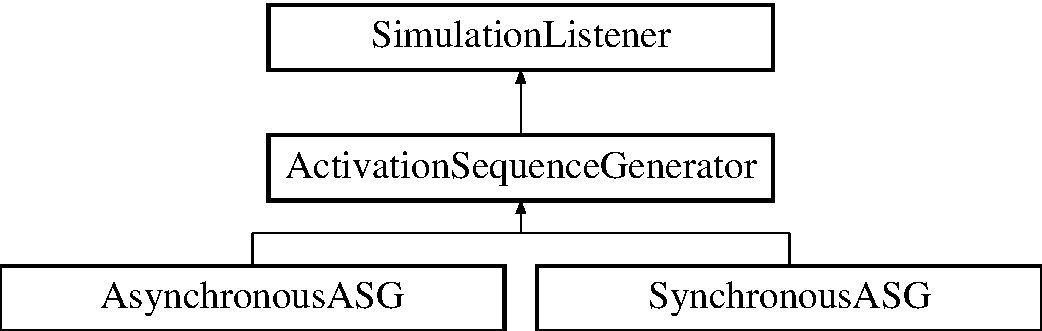
\includegraphics[height=3cm]{class_simulation_listener}
\end{center}
\end{figure}
\subsection*{Public Member Functions}
\begin{CompactItemize}
\item 
virtual void \hyperlink{class_simulation_listener_f1b53fbefce7830648bb059dfd0f18b4}{update} (const \hyperlink{class_world_information}{WorldInformation} \&world\_\-information, boost::shared\_\-ptr$<$ Event $>$ last\_\-event)=0
\end{CompactItemize}


\subsection{Detailed Description}
\hyperlink{class_simulation_listener}{SimulationListener} is an interface to be implemented by classes which wish to be informed of handled events. 

Definition at line 20 of file simulation\_\-listener.h.

\subsection{Member Function Documentation}
\hypertarget{class_simulation_listener_f1b53fbefce7830648bb059dfd0f18b4}{
\index{SimulationListener@{SimulationListener}!update@{update}}
\index{update@{update}!SimulationListener@{SimulationListener}}
\subsubsection[update]{\setlength{\rightskip}{0pt plus 5cm}virtual void SimulationListener::update (const {\bf WorldInformation} \& {\em world\_\-information}, \/  boost::shared\_\-ptr$<$ Event $>$ {\em last\_\-event})\hspace{0.3cm}{\tt  \mbox{[}pure virtual\mbox{]}}}}
\label{class_simulation_listener_f1b53fbefce7830648bb059dfd0f18b4}


updates the listener after a event has happened. World\_\-information is guaranteed to be a pointer to the most recently generated \hyperlink{class_world_information}{WorldInformation} object. It is not guaranteed that last\_\-event is a handle\_\-request event and that world\_\-information was generated for last\_\-event.

\begin{Desc}
\item[Parameters:]
\begin{description}
\item[{\em A}]constant reference to the newest world information \item[{\em The}]last handled event \end{description}
\end{Desc}


Implemented in \hyperlink{class_asynchronous_a_s_g_159110685ece0b48788dcf9d2c085010}{AsynchronousASG}, and \hyperlink{class_synchronous_a_s_g_4b85489783f05e0061c701a1dac51773}{SynchronousASG}.

The documentation for this class was generated from the following file:\begin{CompactItemize}
\item 
src/SimulationKernel/simulation\_\-listener.h\end{CompactItemize}

\hypertarget{class_sphere}{
\section{Sphere Class Reference}
\label{class_sphere}\index{Sphere@{Sphere}}
}
Denotes a sphere-obstacle.  


{\tt \#include $<$sphere.h$>$}

Inheritance diagram for Sphere::\begin{figure}[H]
\begin{center}
\leavevmode
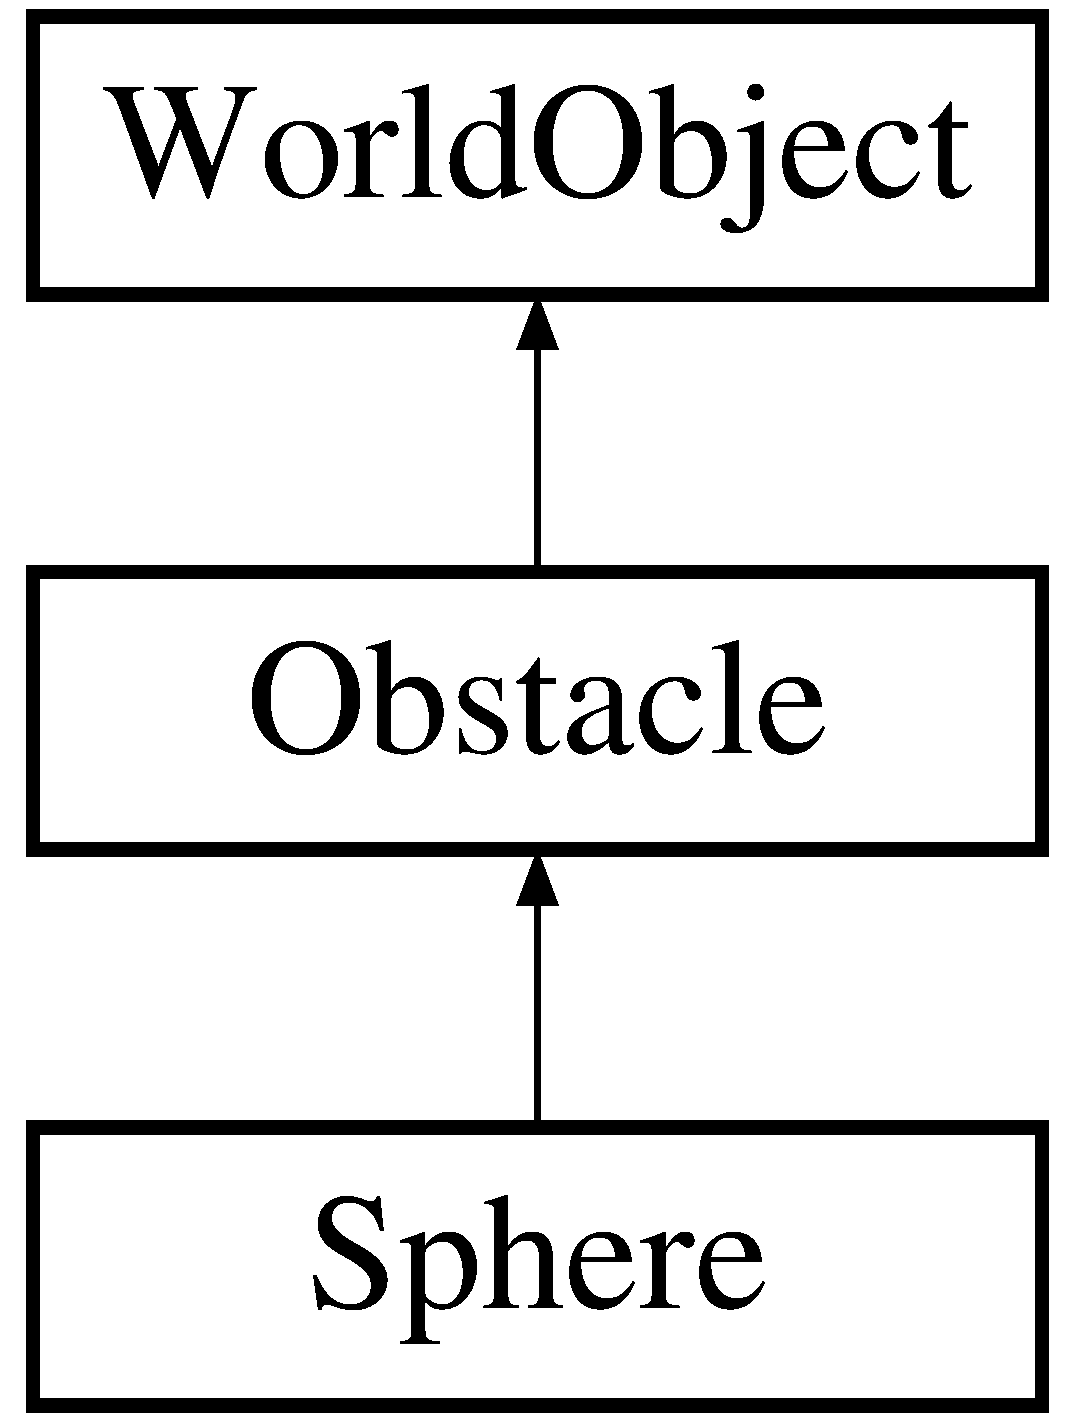
\includegraphics[height=3cm]{class_sphere}
\end{center}
\end{figure}
\subsection*{Public Member Functions}
\begin{CompactItemize}
\item 
\hypertarget{class_sphere_e52b4416e92f208ab754e0d8692091ed}{
\textbf{Sphere} (boost::shared\_\-ptr$<$ \hyperlink{class_identifier}{Identifier} $>$ id, boost::shared\_\-ptr$<$ Vector3d $>$ position, double radius)}
\label{class_sphere_e52b4416e92f208ab754e0d8692091ed}

\item 
\hypertarget{class_sphere_d897b22b306c1b275dafddf22c3d75c8}{
\textbf{Sphere} (boost::shared\_\-ptr$<$ \hyperlink{class_identifier}{Identifier} $>$ id, boost::shared\_\-ptr$<$ Vector3d $>$ position, boost::shared\_\-ptr$<$ \hyperlink{class_marker_information}{MarkerInformation} $>$ marker\_\-information, double radius)}
\label{class_sphere_d897b22b306c1b275dafddf22c3d75c8}

\item 
double \hyperlink{class_sphere_82c3e6746f79196c744b46f39569689e}{radius} () const 
\item 
void \hyperlink{class_sphere_67b1c1595ffd2c0dcf8abfeca8de5c36}{set\_\-radius} (double new\_\-radius)
\item 
bool \hyperlink{class_sphere_f031ce505d4f21bc7d8bf1b7684280e0}{contains\_\-point} (boost::shared\_\-ptr$<$ Vector3d $>$ point) const 
\item 
virtual boost::shared\_\-ptr$<$ \hyperlink{class_world_object}{WorldObject} $>$ \hyperlink{class_sphere_6fcc846dbbef396057b572b9a0786cdc}{clone} () const 
\end{CompactItemize}
\subsection*{Private Attributes}
\begin{CompactItemize}
\item 
\hypertarget{class_sphere_e5bc6962474cb1fb220b7aa956257554}{
double \textbf{radius\_\-}}
\label{class_sphere_e5bc6962474cb1fb220b7aa956257554}

\end{CompactItemize}


\subsection{Detailed Description}
Denotes a sphere-obstacle. 

\begin{Desc}
\item[Author:]Martina Hüllmann \end{Desc}


Definition at line 13 of file sphere.h.

\subsection{Member Function Documentation}
\hypertarget{class_sphere_82c3e6746f79196c744b46f39569689e}{
\index{Sphere@{Sphere}!radius@{radius}}
\index{radius@{radius}!Sphere@{Sphere}}
\subsubsection[radius]{\setlength{\rightskip}{0pt plus 5cm}double Sphere::radius () const}}
\label{class_sphere_82c3e6746f79196c744b46f39569689e}


Returns the radius of the sphere. \begin{Desc}
\item[Returns:]Radius of the sphere. \end{Desc}


Definition at line 27 of file sphere.cc.

Referenced by Octree::determine\_\-obstacle\_\-max\_\-size().\hypertarget{class_sphere_67b1c1595ffd2c0dcf8abfeca8de5c36}{
\index{Sphere@{Sphere}!set\_\-radius@{set\_\-radius}}
\index{set\_\-radius@{set\_\-radius}!Sphere@{Sphere}}
\subsubsection[set\_\-radius]{\setlength{\rightskip}{0pt plus 5cm}void Sphere::set\_\-radius (double {\em new\_\-radius})}}
\label{class_sphere_67b1c1595ffd2c0dcf8abfeca8de5c36}


Sets the radius of the sphere to the given value. \begin{Desc}
\item[Parameters:]
\begin{description}
\item[{\em New}]radius of the sphere. \end{description}
\end{Desc}


Definition at line 31 of file sphere.cc.\hypertarget{class_sphere_f031ce505d4f21bc7d8bf1b7684280e0}{
\index{Sphere@{Sphere}!contains\_\-point@{contains\_\-point}}
\index{contains\_\-point@{contains\_\-point}!Sphere@{Sphere}}
\subsubsection[contains\_\-point]{\setlength{\rightskip}{0pt plus 5cm}bool Sphere::contains\_\-point (boost::shared\_\-ptr$<$ Vector3d $>$ {\em point}) const}}
\label{class_sphere_f031ce505d4f21bc7d8bf1b7684280e0}


Checks whether the given point is contained in the obstacle. \begin{Desc}
\item[Parameters:]
\begin{description}
\item[{\em Pointer}]to vector of point to check whether it's contained in the obstacle. \end{description}
\end{Desc}


Definition at line 35 of file sphere.cc.\hypertarget{class_sphere_6fcc846dbbef396057b572b9a0786cdc}{
\index{Sphere@{Sphere}!clone@{clone}}
\index{clone@{clone}!Sphere@{Sphere}}
\subsubsection[clone]{\setlength{\rightskip}{0pt plus 5cm}boost::shared\_\-ptr$<$ {\bf WorldObject} $>$ Sphere::clone () const\hspace{0.3cm}{\tt  \mbox{[}virtual\mbox{]}}}}
\label{class_sphere_6fcc846dbbef396057b572b9a0786cdc}


Clones this object and returns a shared ptr to the cloned object. typeid($\ast$this) == typeid($\ast$clone) \begin{Desc}
\item[Returns:]shared ptr to the cloned object \end{Desc}


Reimplemented from \hyperlink{class_world_object_dba468299ce77ce5781e60081bf44b14}{WorldObject}.

Definition at line 48 of file sphere.cc.

The documentation for this class was generated from the following files:\begin{CompactItemize}
\item 
src/Model/sphere.h\item 
src/Model/sphere.cc\end{CompactItemize}

\hypertarget{class_sphere_identifier}{
\section{SphereIdentifier Class Reference}
\label{class_sphere_identifier}\index{SphereIdentifier@{SphereIdentifier}}
}
Denote ID's of spheres.  


{\tt \#include $<$sphere\_\-identifier.h$>$}

Inheritance diagram for SphereIdentifier::\begin{figure}[H]
\begin{center}
\leavevmode
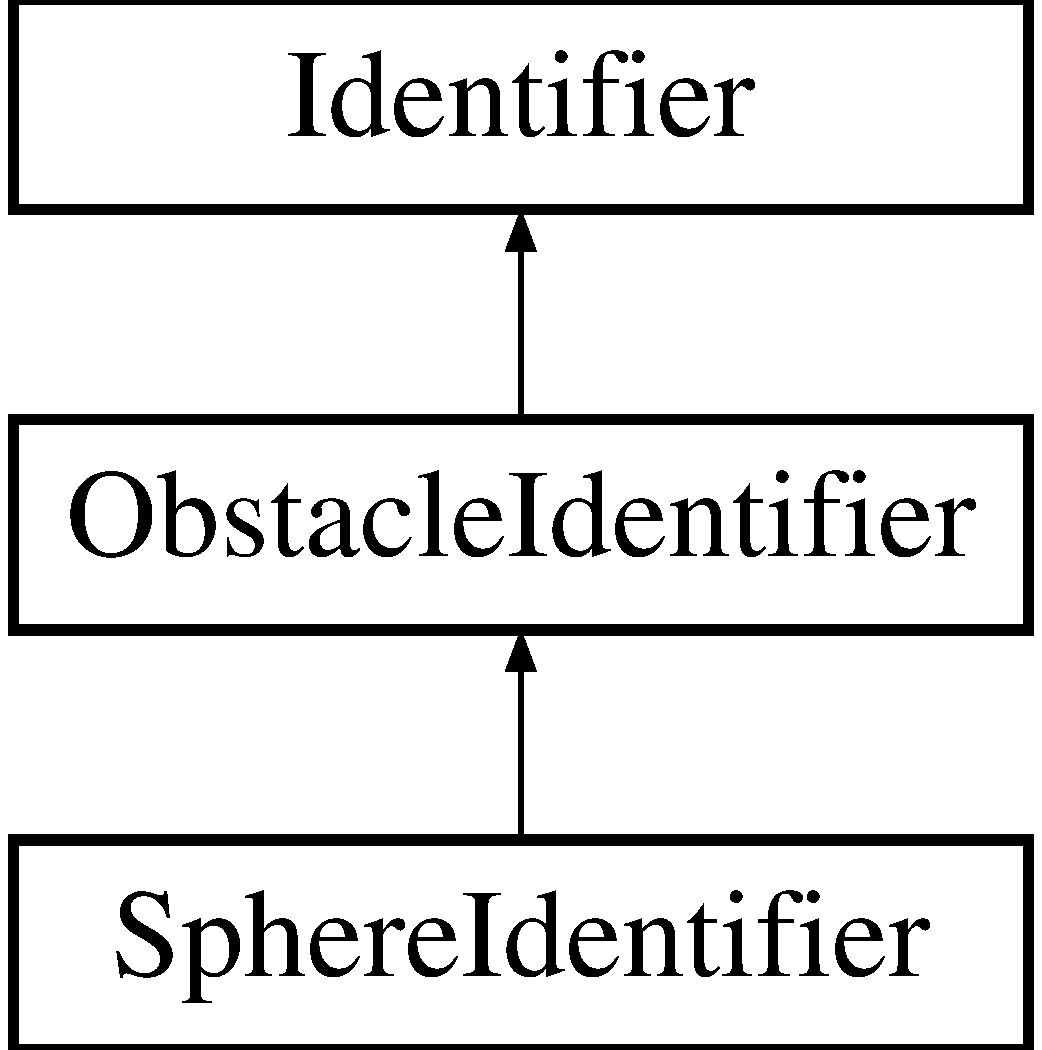
\includegraphics[height=3cm]{class_sphere_identifier}
\end{center}
\end{figure}
\subsection*{Public Member Functions}
\begin{CompactItemize}
\item 
\hypertarget{class_sphere_identifier_e3e16fb0a8e0dfd15ab6c46f7b5661ed}{
virtual boost::shared\_\-ptr$<$ \hyperlink{class_identifier}{Identifier} $>$ \textbf{clone} () const }
\label{class_sphere_identifier_e3e16fb0a8e0dfd15ab6c46f7b5661ed}

\end{CompactItemize}
\subsection*{Protected Member Functions}
\begin{CompactItemize}
\item 
\hypertarget{class_sphere_identifier_d8aa95d39370ed459d385ce79cbb7c5a}{
\textbf{SphereIdentifier} (std::size\_\-t id)}
\label{class_sphere_identifier_d8aa95d39370ed459d385ce79cbb7c5a}

\end{CompactItemize}
\subsection*{Friends}
\begin{CompactItemize}
\item 
\hypertarget{class_sphere_identifier_6433c824d5e64fc5b3635b2a0f2af16c}{
class \textbf{SimpleWorldFixture}}
\label{class_sphere_identifier_6433c824d5e64fc5b3635b2a0f2af16c}

\end{CompactItemize}


\subsection{Detailed Description}
Denote ID's of spheres. 

\begin{Desc}
\item[Author:]Martina Hüllmann \end{Desc}


Definition at line 12 of file sphere\_\-identifier.h.

The documentation for this class was generated from the following files:\begin{CompactItemize}
\item 
src/Model/sphere\_\-identifier.h\item 
src/Model/sphere\_\-identifier.cc\end{CompactItemize}

\hypertarget{class_spheric_view}{
\section{SphericView Class Reference}
\label{class_spheric_view}\index{SphericView@{SphericView}}
}
Basic spherical view model.  


{\tt \#include $<$spheric\_\-view.h$>$}

Inheritance diagram for SphericView::\begin{figure}[H]
\begin{center}
\leavevmode
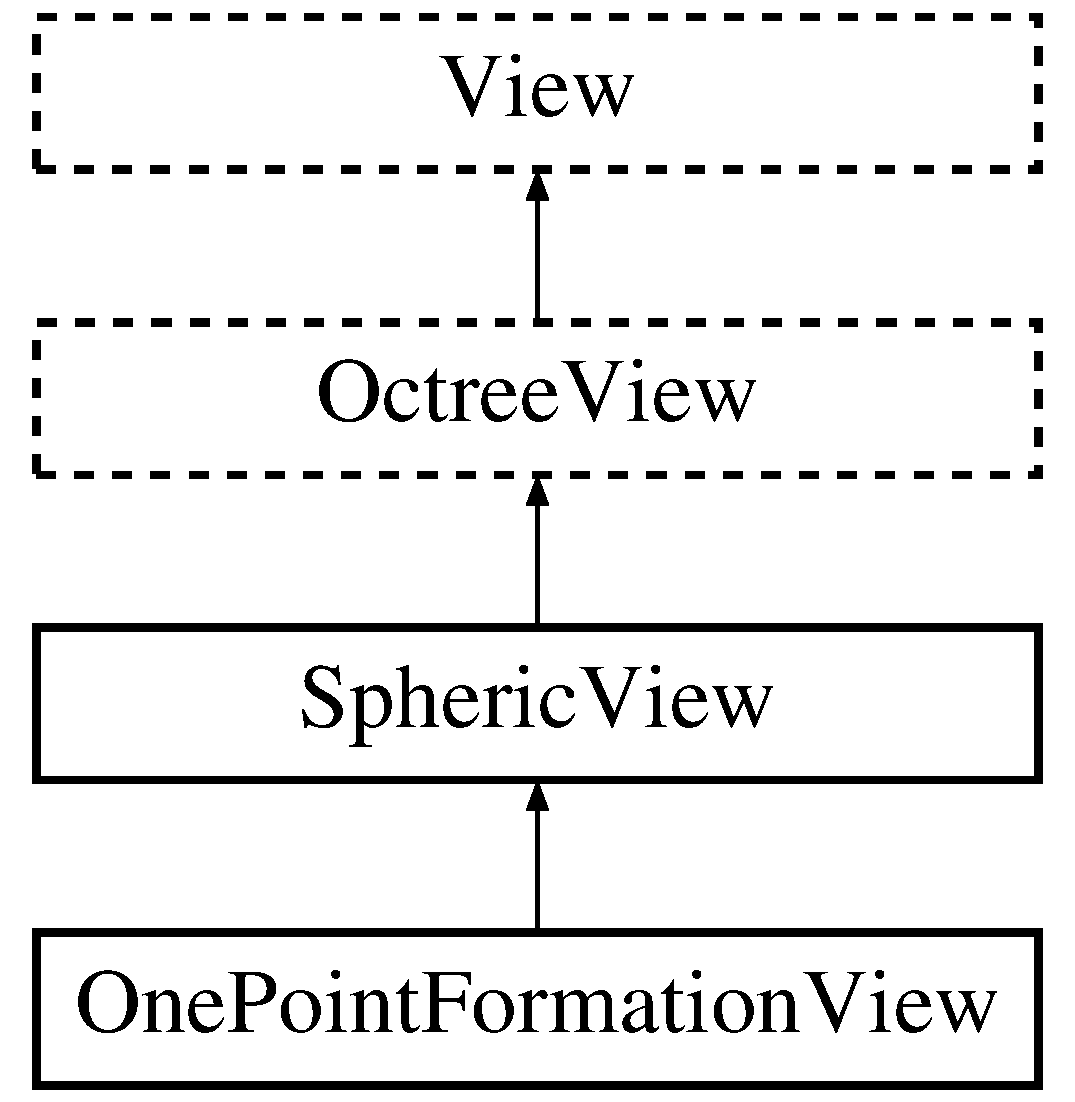
\includegraphics[height=4cm]{class_spheric_view}
\end{center}
\end{figure}
\subsection*{Public Member Functions}
\begin{CompactItemize}
\item 
\hypertarget{class_spheric_view_bfe97f597005a4de0a36ef639990ab63}{
\textbf{SphericView} (double view\_\-radius)}
\label{class_spheric_view_bfe97f597005a4de0a36ef639990ab63}

\item 
void \hyperlink{class_spheric_view_dbd6a1d5e2f17594f82e831c38d35ec6}{init} (const \hyperlink{class_world_information}{WorldInformation} \&world\_\-information)
\end{CompactItemize}
\subsection*{Protected Member Functions}
\begin{CompactItemize}
\item 
\hypertarget{class_spheric_view_432056355d892add503c2950df457209}{
virtual std::set$<$ RobotRef $>$ \textbf{get\_\-visible\_\-robots} (const \hyperlink{class_robot_data}{RobotData} \&robot) const }
\label{class_spheric_view_432056355d892add503c2950df457209}

\item 
\hypertarget{class_spheric_view_63302af51818598dd14b4a41f68424de}{
virtual std::set$<$ ObstacleRef $>$ \textbf{get\_\-visible\_\-obstacles} (const \hyperlink{class_robot_data}{RobotData} \&robot) const }
\label{class_spheric_view_63302af51818598dd14b4a41f68424de}

\item 
\hypertarget{class_spheric_view_daa935af0af47909afd7234f024ab1f2}{
virtual std::set$<$ MarkerRef $>$ \textbf{get\_\-visible\_\-markers} (const \hyperlink{class_robot_data}{RobotData} \&robot) const }
\label{class_spheric_view_daa935af0af47909afd7234f024ab1f2}

\item 
\hypertarget{class_spheric_view_83c5707136239b6c1c7af5fb2f320030}{
double \textbf{view\_\-radius} () const }
\label{class_spheric_view_83c5707136239b6c1c7af5fb2f320030}

\end{CompactItemize}
\subsection*{Private Attributes}
\begin{CompactItemize}
\item 
\hypertarget{class_spheric_view_5145c1290593cd597136d588dae1c060}{
double \textbf{view\_\-radius\_\-}}
\label{class_spheric_view_5145c1290593cd597136d588dae1c060}

\end{CompactItemize}


\subsection{Detailed Description}
Basic spherical view model. 

Provides implementations of getVisible... methods. To efficiently implement them the classes uses an \hyperlink{class_octree}{Octree} as internal data structure.

Assigning this class to a Robot corresponds to a \char`\"{}see all objects in a given radius\char`\"{} model. 

Definition at line 25 of file spheric\_\-view.h.

\subsection{Member Function Documentation}
\hypertarget{class_spheric_view_dbd6a1d5e2f17594f82e831c38d35ec6}{
\index{SphericView@{SphericView}!init@{init}}
\index{init@{init}!SphericView@{SphericView}}
\subsubsection[init]{\setlength{\rightskip}{0pt plus 5cm}void SphericView::init (const {\bf WorldInformation} \& {\em world\_\-information})\hspace{0.3cm}{\tt  \mbox{[}virtual\mbox{]}}}}
\label{class_spheric_view_dbd6a1d5e2f17594f82e831c38d35ec6}


Although init is trivial, it is nice to have a default constructor in virtual inherited classes. Otherwise every arbitrary deep sub class has to call the non-default constructor. Call this method before using any other method of \hyperlink{class_view}{View}. \begin{Desc}
\item[Parameters:]
\begin{description}
\item[{\em \hyperlink{class_world_information}{WorldInformation}}]\end{description}
\end{Desc}


Reimplemented from \hyperlink{class_octree_view_800b8d09dbd898769439f1765e7d87b1}{OctreeView}.

Definition at line 24 of file spheric\_\-view.cc.

References View::init(), WorldInformation::markers(), WorldInformation::obstacles(), and WorldInformation::robot\_\-data().

The documentation for this class was generated from the following files:\begin{CompactItemize}
\item 
src/Views/spheric\_\-view.h\item 
src/Views/spheric\_\-view.cc\end{CompactItemize}

\hypertarget{class_synchronous_a_s_g}{
\section{SynchronousASG Class Reference}
\label{class_synchronous_a_s_g}\index{SynchronousASG@{SynchronousASG}}
}
The synchronous ASG produces a sequence of events according to the fully-synchronous time-model.  


{\tt \#include $<$synchronous\_\-asg.h$>$}

Inheritance diagram for SynchronousASG::\begin{figure}[H]
\begin{center}
\leavevmode
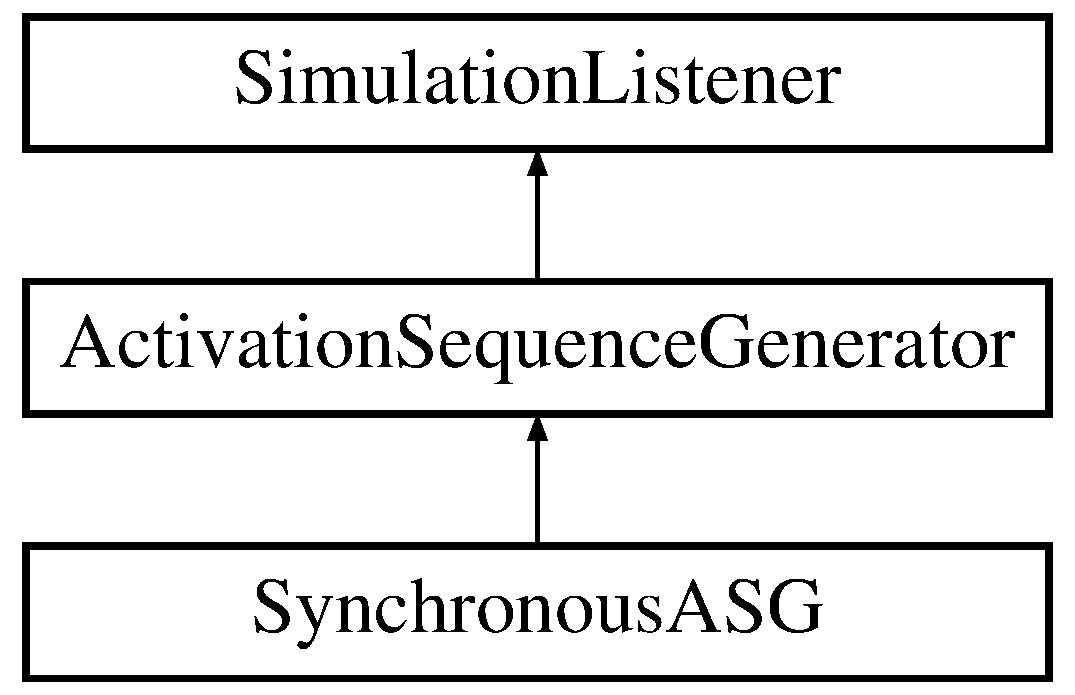
\includegraphics[height=3cm]{class_synchronous_a_s_g}
\end{center}
\end{figure}
\subsection*{Public Member Functions}
\begin{CompactItemize}
\item 
void \hyperlink{class_synchronous_a_s_g_05acba7c914bdb8b4080ef763c092993}{initialize} (const \hyperlink{class_history}{History} \&history, const vector$<$ boost::shared\_\-ptr$<$ Robot $>$ $>$ \&robots)
\item 
boost::shared\_\-ptr$<$ Event $>$ \hyperlink{class_synchronous_a_s_g_05fbdbd3ed9638ab90c3817944fbba95}{get\_\-next\_\-event} ()
\item 
int \hyperlink{class_synchronous_a_s_g_b675d2066e00287119c772b0411531b5}{get\_\-time\_\-of\_\-next\_\-event} ()
\item 
void \hyperlink{class_synchronous_a_s_g_4b85489783f05e0061c701a1dac51773}{update} (const \hyperlink{class_world_information}{WorldInformation} \&world\_\-information, boost::shared\_\-ptr$<$ Event $>$ event)
\end{CompactItemize}
\subsection*{Private Attributes}
\begin{CompactItemize}
\item 
int \hyperlink{class_synchronous_a_s_g_abb2e0b562aea4bc197c54e4a9298918}{time\_\-of\_\-next\_\-event\_\-}
\item 
vector$<$ boost::shared\_\-ptr$<$ const \hyperlink{class_request}{Request} $>$ $>$ \hyperlink{class_synchronous_a_s_g_decb1886c61bad1814a2d76f03b6021c}{unhandled\_\-request\_\-set\_\-}
\item 
vector$<$ boost::shared\_\-ptr$<$ Robot $>$ $>$ \hyperlink{class_synchronous_a_s_g_a2a7e5be2f90c3e875db299d27895346}{robots\_\-}
\end{CompactItemize}
\subsection*{Static Private Attributes}
\begin{CompactItemize}
\item 
\hypertarget{class_synchronous_a_s_g_9127128e60da48154da2e3ef6e8ced85}{
static const int \textbf{kTimeToLook} = 0}
\label{class_synchronous_a_s_g_9127128e60da48154da2e3ef6e8ced85}

\item 
\hypertarget{class_synchronous_a_s_g_87b700024cffa28e67b05abc5fdbab46}{
static const int \textbf{kTimeToCompute} = 1}
\label{class_synchronous_a_s_g_87b700024cffa28e67b05abc5fdbab46}

\item 
\hypertarget{class_synchronous_a_s_g_c9d1ea6a8943c9308c0e238fd1d379ef}{
static const int \textbf{kTimeToMove} = 2}
\label{class_synchronous_a_s_g_c9d1ea6a8943c9308c0e238fd1d379ef}

\item 
\hypertarget{class_synchronous_a_s_g_f5d8677345914ed5c915e331e6796cd8}{
static const int \textbf{kNumberOfEvents} = 3}
\label{class_synchronous_a_s_g_f5d8677345914ed5c915e331e6796cd8}

\end{CompactItemize}


\subsection{Detailed Description}
The synchronous ASG produces a sequence of events according to the fully-synchronous time-model. 

Definition at line 29 of file synchronous\_\-asg.h.

\subsection{Member Function Documentation}
\hypertarget{class_synchronous_a_s_g_05acba7c914bdb8b4080ef763c092993}{
\index{SynchronousASG@{SynchronousASG}!initialize@{initialize}}
\index{initialize@{initialize}!SynchronousASG@{SynchronousASG}}
\subsubsection[initialize]{\setlength{\rightskip}{0pt plus 5cm}void SynchronousASG::initialize (const {\bf History} \& {\em history}, \/  const vector$<$ boost::shared\_\-ptr$<$ Robot $>$ $>$ \& {\em robots})\hspace{0.3cm}{\tt  \mbox{[}virtual\mbox{]}}}}
\label{class_synchronous_a_s_g_05acba7c914bdb8b4080ef763c092993}


initializes the synchronous ASG from the given intial world\_\-state. Needs to be called before the ASG is used \begin{Desc}
\item[Parameters:]
\begin{description}
\item[{\em The}]intial world state \end{description}
\end{Desc}


Implements \hyperlink{class_activation_sequence_generator_01592eb2b4293512d2ad00dc4adf0361}{ActivationSequenceGenerator}.

Definition at line 24 of file synchronous\_\-asg.cc.

References robots\_\-.\hypertarget{class_synchronous_a_s_g_05fbdbd3ed9638ab90c3817944fbba95}{
\index{SynchronousASG@{SynchronousASG}!get\_\-next\_\-event@{get\_\-next\_\-event}}
\index{get\_\-next\_\-event@{get\_\-next\_\-event}!SynchronousASG@{SynchronousASG}}
\subsubsection[get\_\-next\_\-event]{\setlength{\rightskip}{0pt plus 5cm}boost::shared\_\-ptr$<$ Event $>$ SynchronousASG::get\_\-next\_\-event ()\hspace{0.3cm}{\tt  \mbox{[}virtual\mbox{]}}}}
\label{class_synchronous_a_s_g_05fbdbd3ed9638ab90c3817944fbba95}


Returns the next event. Since the ASG is synchronous the sequence of events will have the form of (look-compute-handle\_\-requests)$\ast$. Each look and each compute event applies to every existing robot. In each handle\_\-requests event all outstanding requests from the previous compute event is given to the event handler. \begin{Desc}
\item[Returns:]The next event in the sequence. \end{Desc}


Implements \hyperlink{class_activation_sequence_generator_cf20a8caaee580655c57b8843d82d5f5}{ActivationSequenceGenerator}.

Definition at line 32 of file synchronous\_\-asg.cc.

References HandleRequestsEvent::add\_\-to\_\-requests(), ComputeEvent::add\_\-to\_\-robot\_\-subset(), LookEvent::add\_\-to\_\-robot\_\-subset(), robots\_\-, time\_\-of\_\-next\_\-event\_\-, and unhandled\_\-request\_\-set\_\-.\hypertarget{class_synchronous_a_s_g_b675d2066e00287119c772b0411531b5}{
\index{SynchronousASG@{SynchronousASG}!get\_\-time\_\-of\_\-next\_\-event@{get\_\-time\_\-of\_\-next\_\-event}}
\index{get\_\-time\_\-of\_\-next\_\-event@{get\_\-time\_\-of\_\-next\_\-event}!SynchronousASG@{SynchronousASG}}
\subsubsection[get\_\-time\_\-of\_\-next\_\-event]{\setlength{\rightskip}{0pt plus 5cm}int SynchronousASG::get\_\-time\_\-of\_\-next\_\-event ()\hspace{0.3cm}{\tt  \mbox{[}inline, virtual\mbox{]}}}}
\label{class_synchronous_a_s_g_b675d2066e00287119c772b0411531b5}


Returns the time of the next event. This is always the time of the last event plus one. \begin{Desc}
\item[Returns:]The time of the next event. \end{Desc}


Implements \hyperlink{class_activation_sequence_generator_724cfa2e135813db7becb90af1783050}{ActivationSequenceGenerator}.

Definition at line 53 of file synchronous\_\-asg.h.

References time\_\-of\_\-next\_\-event\_\-.\hypertarget{class_synchronous_a_s_g_4b85489783f05e0061c701a1dac51773}{
\index{SynchronousASG@{SynchronousASG}!update@{update}}
\index{update@{update}!SynchronousASG@{SynchronousASG}}
\subsubsection[update]{\setlength{\rightskip}{0pt plus 5cm}void SynchronousASG::update (const {\bf WorldInformation} \& {\em world\_\-information}, \/  boost::shared\_\-ptr$<$ Event $>$ {\em event})\hspace{0.3cm}{\tt  \mbox{[}virtual\mbox{]}}}}
\label{class_synchronous_a_s_g_4b85489783f05e0061c701a1dac51773}


Updates the sequence of events. For the synchronous ASG this only stores the requests of robots stored in compute events. The requests are added to the next handle\_\-requests event. \begin{Desc}
\item[Parameters:]
\begin{description}
\item[{\em A}]constant refrence to the newest world information \item[{\em The}]last handled event \end{description}
\end{Desc}


Implements \hyperlink{class_simulation_listener_f1b53fbefce7830648bb059dfd0f18b4}{SimulationListener}.

Definition at line 68 of file synchronous\_\-asg.cc.

References ComputeEvent::requests(), and unhandled\_\-request\_\-set\_\-.

\subsection{Member Data Documentation}
\hypertarget{class_synchronous_a_s_g_abb2e0b562aea4bc197c54e4a9298918}{
\index{SynchronousASG@{SynchronousASG}!time\_\-of\_\-next\_\-event\_\-@{time\_\-of\_\-next\_\-event\_\-}}
\index{time\_\-of\_\-next\_\-event\_\-@{time\_\-of\_\-next\_\-event\_\-}!SynchronousASG@{SynchronousASG}}
\subsubsection[time\_\-of\_\-next\_\-event\_\-]{\setlength{\rightskip}{0pt plus 5cm}int {\bf SynchronousASG::time\_\-of\_\-next\_\-event\_\-}\hspace{0.3cm}{\tt  \mbox{[}private\mbox{]}}}}
\label{class_synchronous_a_s_g_abb2e0b562aea4bc197c54e4a9298918}


The time the next event will happen. 

Definition at line 68 of file synchronous\_\-asg.h.

Referenced by get\_\-next\_\-event(), and get\_\-time\_\-of\_\-next\_\-event().\hypertarget{class_synchronous_a_s_g_decb1886c61bad1814a2d76f03b6021c}{
\index{SynchronousASG@{SynchronousASG}!unhandled\_\-request\_\-set\_\-@{unhandled\_\-request\_\-set\_\-}}
\index{unhandled\_\-request\_\-set\_\-@{unhandled\_\-request\_\-set\_\-}!SynchronousASG@{SynchronousASG}}
\subsubsection[unhandled\_\-request\_\-set\_\-]{\setlength{\rightskip}{0pt plus 5cm}vector$<$boost::shared\_\-ptr$<$const {\bf Request}$>$ $>$ {\bf SynchronousASG::unhandled\_\-request\_\-set\_\-}\hspace{0.3cm}{\tt  \mbox{[}private\mbox{]}}}}
\label{class_synchronous_a_s_g_decb1886c61bad1814a2d76f03b6021c}


A set of unhandled requests from the last compute event. 

Definition at line 73 of file synchronous\_\-asg.h.

Referenced by get\_\-next\_\-event(), and update().\hypertarget{class_synchronous_a_s_g_a2a7e5be2f90c3e875db299d27895346}{
\index{SynchronousASG@{SynchronousASG}!robots\_\-@{robots\_\-}}
\index{robots\_\-@{robots\_\-}!SynchronousASG@{SynchronousASG}}
\subsubsection[robots\_\-]{\setlength{\rightskip}{0pt plus 5cm}vector$<$boost::shared\_\-ptr$<$Robot$>$ $>$ {\bf SynchronousASG::robots\_\-}\hspace{0.3cm}{\tt  \mbox{[}private\mbox{]}}}}
\label{class_synchronous_a_s_g_a2a7e5be2f90c3e875db299d27895346}


The set of all robots 

Definition at line 78 of file synchronous\_\-asg.h.

Referenced by get\_\-next\_\-event(), and initialize().

The documentation for this class was generated from the following files:\begin{CompactItemize}
\item 
src/ActivationSequenceGenerators/synchronous\_\-asg.h\item 
src/ActivationSequenceGenerators/synchronous\_\-asg.cc\end{CompactItemize}

\hypertarget{class_type_change_request}{
\section{TypeChangeRequest Class Reference}
\label{class_type_change_request}\index{TypeChangeRequest@{TypeChangeRequest}}
}
A Type Change \hyperlink{class_request}{Request} is issued by a robot which wants to change its type (e.g. become leader).  


{\tt \#include $<$type\_\-change\_\-request.h$>$}

Inheritance diagram for TypeChangeRequest::\begin{figure}[H]
\begin{center}
\leavevmode
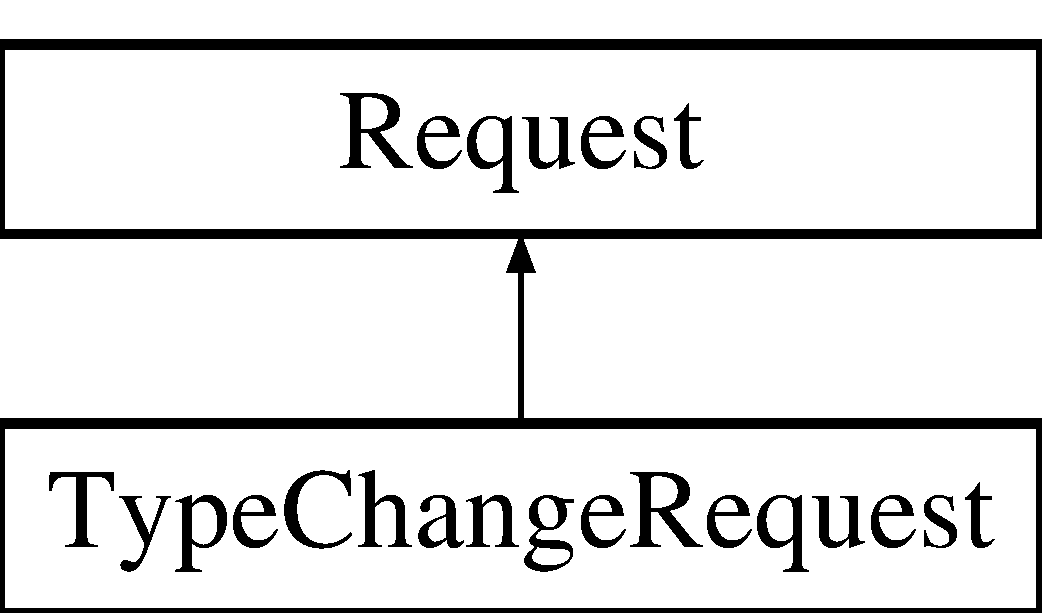
\includegraphics[height=2cm]{class_type_change_request}
\end{center}
\end{figure}
\subsection*{Public Member Functions}
\begin{CompactItemize}
\item 
\hyperlink{class_type_change_request_2722d08bb752b22163f2cb0fd82e1d6d}{TypeChangeRequest} (Robot \&robot, RobotType requested\_\-type)
\item 
const RobotType \& \hyperlink{class_type_change_request_bba308af9b35aa89b2feb9665249ea9a}{requested\_\-type} () const 
\end{CompactItemize}
\subsection*{Private Attributes}
\begin{CompactItemize}
\item 
\hypertarget{class_type_change_request_612c0385a16030c01d4324080408c52f}{
RobotType \textbf{requested\_\-type\_\-}}
\label{class_type_change_request_612c0385a16030c01d4324080408c52f}

\end{CompactItemize}


\subsection{Detailed Description}
A Type Change \hyperlink{class_request}{Request} is issued by a robot which wants to change its type (e.g. become leader). 

Notes: This request differs from the other request classes since it doesn't take a pointer to the requested type but rather the type directly. Since Type is only a small enum we don't need the overhead of the shared pointer.

The request cannot be changed after creating. 

Definition at line 25 of file type\_\-change\_\-request.h.

\subsection{Constructor \& Destructor Documentation}
\hypertarget{class_type_change_request_2722d08bb752b22163f2cb0fd82e1d6d}{
\index{TypeChangeRequest@{TypeChangeRequest}!TypeChangeRequest@{TypeChangeRequest}}
\index{TypeChangeRequest@{TypeChangeRequest}!TypeChangeRequest@{TypeChangeRequest}}
\subsubsection[TypeChangeRequest]{\setlength{\rightskip}{0pt plus 5cm}TypeChangeRequest::TypeChangeRequest (Robot \& {\em robot}, \/  RobotType {\em requested\_\-type})\hspace{0.3cm}{\tt  \mbox{[}inline\mbox{]}}}}
\label{class_type_change_request_2722d08bb752b22163f2cb0fd82e1d6d}


Constructs a new type change request. The request cannot be changed after construction. 

Definition at line 31 of file type\_\-change\_\-request.h.

\subsection{Member Function Documentation}
\hypertarget{class_type_change_request_bba308af9b35aa89b2feb9665249ea9a}{
\index{TypeChangeRequest@{TypeChangeRequest}!requested\_\-type@{requested\_\-type}}
\index{requested\_\-type@{requested\_\-type}!TypeChangeRequest@{TypeChangeRequest}}
\subsubsection[requested\_\-type]{\setlength{\rightskip}{0pt plus 5cm}const RobotType\& TypeChangeRequest::requested\_\-type () const\hspace{0.3cm}{\tt  \mbox{[}inline\mbox{]}}}}
\label{class_type_change_request_bba308af9b35aa89b2feb9665249ea9a}


Returns a constant reference to the requested type \begin{Desc}
\item[Returns:]A constant reference to the requested type \end{Desc}


Definition at line 38 of file type\_\-change\_\-request.h.

The documentation for this class was generated from the following file:\begin{CompactItemize}
\item 
src/Requests/type\_\-change\_\-request.h\end{CompactItemize}

\hypertarget{class_type_change_request_handler}{
\section{TypeChangeRequestHandler Class Reference}
\label{class_type_change_request_handler}\index{TypeChangeRequestHandler@{TypeChangeRequestHandler}}
}
{\tt \#include $<$type\_\-change\_\-request\_\-handler.h$>$}

Inheritance diagram for TypeChangeRequestHandler::\begin{figure}[H]
\begin{center}
\leavevmode
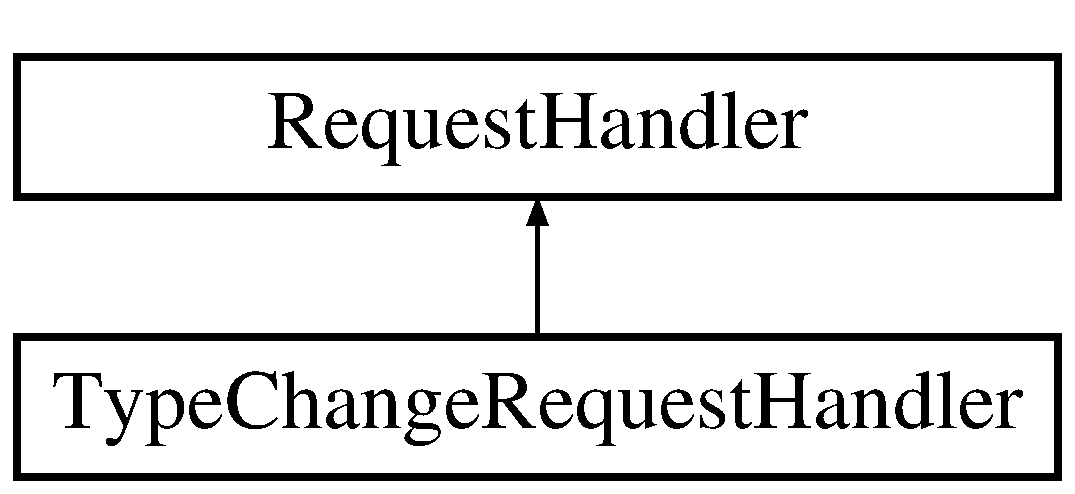
\includegraphics[height=2cm]{class_type_change_request_handler}
\end{center}
\end{figure}
\subsection*{Public Member Functions}
\begin{CompactItemize}
\item 
\hypertarget{class_type_change_request_handler_c832f59730866b2a7dda685358743ac6}{
\textbf{TypeChangeRequestHandler} (unsigned int seed, double discard\_\-probability, const \hyperlink{class_history}{History} \&history)}
\label{class_type_change_request_handler_c832f59730866b2a7dda685358743ac6}

\end{CompactItemize}
\subsection*{Private Member Functions}
\begin{CompactItemize}
\item 
\hypertarget{class_type_change_request_handler_d6e47777fcdb40fe034b0e745364649c}{
virtual void \textbf{handle\_\-request\_\-reliable} (boost::shared\_\-ptr$<$ \hyperlink{class_world_information}{WorldInformation} $>$ world\_\-information, boost::shared\_\-ptr$<$ const \hyperlink{class_request}{Request} $>$ request)}
\label{class_type_change_request_handler_d6e47777fcdb40fe034b0e745364649c}

\end{CompactItemize}


\subsection{Detailed Description}
Standard type change request handler. Fullfills every type change request. 

Definition at line 16 of file type\_\-change\_\-request\_\-handler.h.

The documentation for this class was generated from the following files:\begin{CompactItemize}
\item 
src/EventHandlers/type\_\-change\_\-request\_\-handler.h\item 
src/EventHandlers/type\_\-change\_\-request\_\-handler.cc\end{CompactItemize}

\hypertarget{class_vec_set_stats}{
\section{VecSetStats Class Reference}
\label{class_vec_set_stats}\index{VecSetStats@{VecSetStats}}
}
creates information on a set of Vector3d  


{\tt \#include $<$vecset\_\-stats.h$>$}

\subsection*{Public Member Functions}
\begin{CompactItemize}
\item 
\hyperlink{class_vec_set_stats_c4f1f328da6ba34452e433c6d28b313a}{VecSetStats} ()
\item 
\hyperlink{class_vec_set_stats_15b02682930db0edc827dfcdcfbfcf69}{VecSetStats} (int cfg)
\item 
void \hyperlink{class_vec_set_stats_cf9ea6b5b6b3880f6a55f68c3546b859}{handle} (const std::vector$<$ boost::shared\_\-ptr$<$ Vector3d $>$ $>$ \&data)
\item 
const int \hyperlink{class_vec_set_stats_8d51d3b79744c15c0fa669abbad1d469}{cfg} () const 
\item 
void \hyperlink{class_vec_set_stats_41912c77a81f3fbaeaf15dbdcdb4b4b8}{set\_\-cfg} (int cfg)
\item 
const Vector3d \& \hyperlink{class_vec_set_stats_dddc218d55693faa61892774a28b1929}{sum} () const 
\item 
const Vector3d \& \hyperlink{class_vec_set_stats_cb1197a75e96a53182cc0904312240b3}{sumnorm} () const 
\item 
const double \hyperlink{class_vec_set_stats_c3cb153b88e051899d7d731181bef46c}{sumlen} () const 
\item 
const Vector3d \& \hyperlink{class_vec_set_stats_9b87664854b8b4eaf4d4a9b7ce6dd9dd}{avg} () const 
\item 
const Vector3d \& \hyperlink{class_vec_set_stats_7a17760a90c4ae82919f7976df427ba2}{avgnorm} () const 
\item 
const double \hyperlink{class_vec_set_stats_823c982b6d964b040bcd0afe5623ae5a}{avglen} () const 
\item 
const Vector3d \& \hyperlink{class_vec_set_stats_6fb6a02bbdabbcfb815cdb591c850030}{shortest} () const 
\item 
const double \hyperlink{class_vec_set_stats_b91c568dbcd9cd91a16f2610af2b66aa}{shortestlen} () const 
\item 
const Vector3d \& \hyperlink{class_vec_set_stats_c5e5192e85e5633cdedf4900f46adb1d}{longest} () const 
\item 
const double \hyperlink{class_vec_set_stats_746c64887edd603e6bf6d139078f8a5c}{longestlen} () const 
\item 
const double \hyperlink{class_vec_set_stats_bada15ff01d5ab8b4a5addae68cd8b02}{cumullen} () const 
\item 
const std::string \hyperlink{class_vec_set_stats_1618681fee0ab61e61243be352a4cee5}{to\_\-string} () const 
\end{CompactItemize}
\subsection*{Static Public Attributes}
\begin{CompactItemize}
\item 
static const int \hyperlink{class_vec_set_stats_d40b4c031735e61869d380bec761041a}{SUM} = 0x01
\item 
static const int \hyperlink{class_vec_set_stats_5c6b167522f05f04d0357f9c525404ed}{SUMNORM} = 0x02
\item 
static const int \hyperlink{class_vec_set_stats_1a5991a18254611aec6ea124f916b650}{SUMLEN} = 0x04
\item 
static const int \hyperlink{class_vec_set_stats_8d4885dfc7b4e4d631e12b1031dabfa8}{AVG} = 0x08
\item 
static const int \hyperlink{class_vec_set_stats_0972452644e7552d3de11d9763f04d13}{AVGNORM} = 0x10
\item 
static const int \hyperlink{class_vec_set_stats_6d85082797085df8918a799163244e20}{AVGLEN} = 0x20
\item 
static const int \hyperlink{class_vec_set_stats_5ec901fadff91737ffd16ca3d89e08f2}{SHORTEST} = 0x40
\item 
static const int \hyperlink{class_vec_set_stats_3023bfabad5006b6dce50482725a2319}{SHORTEST\_\-LEN} = 0x80
\item 
static const int \hyperlink{class_vec_set_stats_0be7215a7373552c5fabd78881735003}{LONGEST} = 0x100
\item 
static const int \hyperlink{class_vec_set_stats_6fcd640961e61b328785f8c030e30181}{LONGEST\_\-LEN} = 0x200
\item 
static const int \hyperlink{class_vec_set_stats_8fe79d213b693917d14bcacd86ff62aa}{CUMUL\_\-LEN} = 0x400
\item 
static const int \hyperlink{class_vec_set_stats_dd7f69167d67da63e03c36f57335c92c}{DEFAULT} = \hyperlink{class_vec_set_stats_d40b4c031735e61869d380bec761041a}{SUM}$|$\hyperlink{class_vec_set_stats_8d4885dfc7b4e4d631e12b1031dabfa8}{AVG}$|$\hyperlink{class_vec_set_stats_5ec901fadff91737ffd16ca3d89e08f2}{SHORTEST}$|$\hyperlink{class_vec_set_stats_0be7215a7373552c5fabd78881735003}{LONGEST}
\item 
static const int \hyperlink{class_vec_set_stats_b56c7865a2064a85a8e46d6add9bda9f}{ALL} = 0xFFFFFFFF
\end{CompactItemize}
\subsection*{Private Member Functions}
\begin{CompactItemize}
\item 
void \hyperlink{class_vec_set_stats_37fbc88237b5eb4d2ec81656bbf2ecc1}{init} ()
\item 
const double \hyperlink{class_vec_set_stats_e33f29edbe292df8f90a7baed6875d4c}{vec\_\-len} (const Vector3d \&vec) const 
\item 
const std::string \hyperlink{class_vec_set_stats_65b3c5457a2fe6b5fa784263356ab8ac}{to\_\-string} (const Vector3d \&vec) const 
\end{CompactItemize}
\subsection*{Private Attributes}
\begin{CompactItemize}
\item 
int \hyperlink{class_vec_set_stats_c389362aaab290a37301168295c1bb07}{cfg\_\-}
\item 
Vector3d \hyperlink{class_vec_set_stats_6b267c33c513e2ca267d1e75e54828dd}{sum\_\-}
\item 
\hypertarget{class_vec_set_stats_43cfe7e1b1a01a7e46682782741f3ba8}{
Vector3d \textbf{sumnorm\_\-}}
\label{class_vec_set_stats_43cfe7e1b1a01a7e46682782741f3ba8}

\item 
\hypertarget{class_vec_set_stats_7dd2bb9237bb3d5319a7123f6c9bb5f7}{
Vector3d \textbf{avg\_\-}}
\label{class_vec_set_stats_7dd2bb9237bb3d5319a7123f6c9bb5f7}

\item 
\hypertarget{class_vec_set_stats_eecd2407a225f3adebe9c5c673c0dd9a}{
Vector3d \textbf{avgnorm\_\-}}
\label{class_vec_set_stats_eecd2407a225f3adebe9c5c673c0dd9a}

\item 
\hypertarget{class_vec_set_stats_eea888e9caf34a5a03049f2882fb098e}{
Vector3d \textbf{shortest\_\-}}
\label{class_vec_set_stats_eea888e9caf34a5a03049f2882fb098e}

\item 
\hypertarget{class_vec_set_stats_84e222df5cffb87fa471e100993469b3}{
Vector3d \textbf{longest\_\-}}
\label{class_vec_set_stats_84e222df5cffb87fa471e100993469b3}

\item 
\hypertarget{class_vec_set_stats_1bcb8977d966b38050bf48eee16ff6dd}{
double \textbf{sumlen\_\-}}
\label{class_vec_set_stats_1bcb8977d966b38050bf48eee16ff6dd}

\item 
\hypertarget{class_vec_set_stats_b660e97626286d70e381fe3df33b4220}{
double \textbf{avglen\_\-}}
\label{class_vec_set_stats_b660e97626286d70e381fe3df33b4220}

\item 
\hypertarget{class_vec_set_stats_5915bff1a81fa0ae62d8f3c1bc7dc213}{
double \textbf{shortestlen\_\-}}
\label{class_vec_set_stats_5915bff1a81fa0ae62d8f3c1bc7dc213}

\item 
\hypertarget{class_vec_set_stats_f802bcd03f9504792ca0d7d75b388015}{
double \textbf{longestlen\_\-}}
\label{class_vec_set_stats_f802bcd03f9504792ca0d7d75b388015}

\item 
\hypertarget{class_vec_set_stats_e54054f7d22ab2c2e8c7295bf8f1dc9b}{
double \textbf{cumullen\_\-}}
\label{class_vec_set_stats_e54054f7d22ab2c2e8c7295bf8f1dc9b}

\end{CompactItemize}


\subsection{Detailed Description}
creates information on a set of Vector3d 

\begin{Desc}
\item[Author:]Sven Kurras 1. create an instance of this class 2. configure it by a $|$$|$-combination of the various bitflags that are given as static ints in the class. Pass the configuration to the constructor or to set\_\-cfg(...)-function. 3. call handle(...) on a vector of Vector3d to analyse. The currently configured information will now become (re)calculated. 4. read out the information by the respective getter-function or get an overview of all configured information by the \hyperlink{class_vec_set_stats_1618681fee0ab61e61243be352a4cee5}{to\_\-string()}-function. 5. continue with any of the points above. \end{Desc}


Definition at line 23 of file vecset\_\-stats.h.

\subsection{Constructor \& Destructor Documentation}
\hypertarget{class_vec_set_stats_c4f1f328da6ba34452e433c6d28b313a}{
\index{VecSetStats@{VecSetStats}!VecSetStats@{VecSetStats}}
\index{VecSetStats@{VecSetStats}!VecSetStats@{VecSetStats}}
\subsubsection[VecSetStats]{\setlength{\rightskip}{0pt plus 5cm}VecSetStats::VecSetStats ()\hspace{0.3cm}{\tt  \mbox{[}explicit\mbox{]}}}}
\label{class_vec_set_stats_c4f1f328da6ba34452e433c6d28b313a}


default constructor 

Definition at line 3 of file vecset\_\-stats.cc.

References cfg\_\-, and DEFAULT.\hypertarget{class_vec_set_stats_15b02682930db0edc827dfcdcfbfcf69}{
\index{VecSetStats@{VecSetStats}!VecSetStats@{VecSetStats}}
\index{VecSetStats@{VecSetStats}!VecSetStats@{VecSetStats}}
\subsubsection[VecSetStats]{\setlength{\rightskip}{0pt plus 5cm}VecSetStats::VecSetStats (int {\em cfg})\hspace{0.3cm}{\tt  \mbox{[}explicit\mbox{]}}}}
\label{class_vec_set_stats_15b02682930db0edc827dfcdcfbfcf69}


constructor with initial configuration \begin{Desc}
\item[Parameters:]
\begin{description}
\item[{\em the}]cfg-flag-combination to use \end{description}
\end{Desc}


Definition at line 7 of file vecset\_\-stats.cc.

References cfg\_\-.

\subsection{Member Function Documentation}
\hypertarget{class_vec_set_stats_cf9ea6b5b6b3880f6a55f68c3546b859}{
\index{VecSetStats@{VecSetStats}!handle@{handle}}
\index{handle@{handle}!VecSetStats@{VecSetStats}}
\subsubsection[handle]{\setlength{\rightskip}{0pt plus 5cm}void VecSetStats::handle (const std::vector$<$ boost::shared\_\-ptr$<$ Vector3d $>$ $>$ \& {\em data})}}
\label{class_vec_set_stats_cf9ea6b5b6b3880f6a55f68c3546b859}


Calculates all information on all the Vector3D in this std::vector that is requested by the currently set flags. Access the individual information via the respective getter-function, or all combined as a string via the \hyperlink{class_vec_set_stats_1618681fee0ab61e61243be352a4cee5}{to\_\-string()}-function. \begin{Desc}
\item[Parameters:]
\begin{description}
\item[{\em data}]the vectorial data to analyse \end{description}
\end{Desc}


Definition at line 30 of file vecset\_\-stats.cc.

References AVG, AVGLEN, AVGNORM, cfg\_\-, init(), LONGEST, LONGEST\_\-LEN, SHORTEST, SHORTEST\_\-LEN, SUM, sum\_\-, SUMLEN, SUMNORM, and vec\_\-len().\hypertarget{class_vec_set_stats_8d51d3b79744c15c0fa669abbad1d469}{
\index{VecSetStats@{VecSetStats}!cfg@{cfg}}
\index{cfg@{cfg}!VecSetStats@{VecSetStats}}
\subsubsection[cfg]{\setlength{\rightskip}{0pt plus 5cm}const int VecSetStats::cfg () const}}
\label{class_vec_set_stats_8d51d3b79744c15c0fa669abbad1d469}


\begin{Desc}
\item[Returns:]current configuration-flags \end{Desc}


Definition at line 14 of file vecset\_\-stats.cc.

References cfg\_\-.\hypertarget{class_vec_set_stats_41912c77a81f3fbaeaf15dbdcdb4b4b8}{
\index{VecSetStats@{VecSetStats}!set\_\-cfg@{set\_\-cfg}}
\index{set\_\-cfg@{set\_\-cfg}!VecSetStats@{VecSetStats}}
\subsubsection[set\_\-cfg]{\setlength{\rightskip}{0pt plus 5cm}void VecSetStats::set\_\-cfg (int {\em cfg})}}
\label{class_vec_set_stats_41912c77a81f3fbaeaf15dbdcdb4b4b8}


\begin{Desc}
\item[Parameters:]
\begin{description}
\item[{\em cfg}]new configuration-flags to use \end{description}
\end{Desc}


Definition at line 18 of file vecset\_\-stats.cc.

References cfg\_\-.\hypertarget{class_vec_set_stats_dddc218d55693faa61892774a28b1929}{
\index{VecSetStats@{VecSetStats}!sum@{sum}}
\index{sum@{sum}!VecSetStats@{VecSetStats}}
\subsubsection[sum]{\setlength{\rightskip}{0pt plus 5cm}const Vector3d \& VecSetStats::sum () const}}
\label{class_vec_set_stats_dddc218d55693faa61892774a28b1929}


\begin{Desc}
\item[Returns:]constant reference to latest calculated sum-vector, unspecified if not calculated \end{Desc}


Definition at line 97 of file vecset\_\-stats.cc.

References sum\_\-.\hypertarget{class_vec_set_stats_cb1197a75e96a53182cc0904312240b3}{
\index{VecSetStats@{VecSetStats}!sumnorm@{sumnorm}}
\index{sumnorm@{sumnorm}!VecSetStats@{VecSetStats}}
\subsubsection[sumnorm]{\setlength{\rightskip}{0pt plus 5cm}const Vector3d \& VecSetStats::sumnorm () const}}
\label{class_vec_set_stats_cb1197a75e96a53182cc0904312240b3}


\begin{Desc}
\item[Returns:]constant reference to latest calculated normalized sum-vector, unspecified if not calculated \end{Desc}


Definition at line 101 of file vecset\_\-stats.cc.\hypertarget{class_vec_set_stats_c3cb153b88e051899d7d731181bef46c}{
\index{VecSetStats@{VecSetStats}!sumlen@{sumlen}}
\index{sumlen@{sumlen}!VecSetStats@{VecSetStats}}
\subsubsection[sumlen]{\setlength{\rightskip}{0pt plus 5cm}const double VecSetStats::sumlen () const}}
\label{class_vec_set_stats_c3cb153b88e051899d7d731181bef46c}


\begin{Desc}
\item[Returns:]latest calculated sum-vector's length, unspecified if not calculated \end{Desc}


Definition at line 105 of file vecset\_\-stats.cc.\hypertarget{class_vec_set_stats_9b87664854b8b4eaf4d4a9b7ce6dd9dd}{
\index{VecSetStats@{VecSetStats}!avg@{avg}}
\index{avg@{avg}!VecSetStats@{VecSetStats}}
\subsubsection[avg]{\setlength{\rightskip}{0pt plus 5cm}const Vector3d \& VecSetStats::avg () const}}
\label{class_vec_set_stats_9b87664854b8b4eaf4d4a9b7ce6dd9dd}


\begin{Desc}
\item[Returns:]constant reference to latest calculated average-vector, unspecified if not calculated \end{Desc}


Definition at line 109 of file vecset\_\-stats.cc.\hypertarget{class_vec_set_stats_7a17760a90c4ae82919f7976df427ba2}{
\index{VecSetStats@{VecSetStats}!avgnorm@{avgnorm}}
\index{avgnorm@{avgnorm}!VecSetStats@{VecSetStats}}
\subsubsection[avgnorm]{\setlength{\rightskip}{0pt plus 5cm}const Vector3d \& VecSetStats::avgnorm () const}}
\label{class_vec_set_stats_7a17760a90c4ae82919f7976df427ba2}


\begin{Desc}
\item[Returns:]constant reference to latest calculated normalized average-vector, unspecified if not calculated \end{Desc}


Definition at line 113 of file vecset\_\-stats.cc.\hypertarget{class_vec_set_stats_823c982b6d964b040bcd0afe5623ae5a}{
\index{VecSetStats@{VecSetStats}!avglen@{avglen}}
\index{avglen@{avglen}!VecSetStats@{VecSetStats}}
\subsubsection[avglen]{\setlength{\rightskip}{0pt plus 5cm}const double VecSetStats::avglen () const}}
\label{class_vec_set_stats_823c982b6d964b040bcd0afe5623ae5a}


\begin{Desc}
\item[Returns:]latest calculated average-vector's length, unspecified if not calculated \end{Desc}


Definition at line 117 of file vecset\_\-stats.cc.\hypertarget{class_vec_set_stats_6fb6a02bbdabbcfb815cdb591c850030}{
\index{VecSetStats@{VecSetStats}!shortest@{shortest}}
\index{shortest@{shortest}!VecSetStats@{VecSetStats}}
\subsubsection[shortest]{\setlength{\rightskip}{0pt plus 5cm}const Vector3d \& VecSetStats::shortest () const}}
\label{class_vec_set_stats_6fb6a02bbdabbcfb815cdb591c850030}


\begin{Desc}
\item[Returns:]constant reference to latest calculated shortest vector, unspecified if not calculated \end{Desc}


Definition at line 121 of file vecset\_\-stats.cc.\hypertarget{class_vec_set_stats_b91c568dbcd9cd91a16f2610af2b66aa}{
\index{VecSetStats@{VecSetStats}!shortestlen@{shortestlen}}
\index{shortestlen@{shortestlen}!VecSetStats@{VecSetStats}}
\subsubsection[shortestlen]{\setlength{\rightskip}{0pt plus 5cm}const double VecSetStats::shortestlen () const}}
\label{class_vec_set_stats_b91c568dbcd9cd91a16f2610af2b66aa}


\begin{Desc}
\item[Returns:]latest calculated shortest vector's length, unspecified if not calculated \end{Desc}


Definition at line 125 of file vecset\_\-stats.cc.\hypertarget{class_vec_set_stats_c5e5192e85e5633cdedf4900f46adb1d}{
\index{VecSetStats@{VecSetStats}!longest@{longest}}
\index{longest@{longest}!VecSetStats@{VecSetStats}}
\subsubsection[longest]{\setlength{\rightskip}{0pt plus 5cm}const Vector3d \& VecSetStats::longest () const}}
\label{class_vec_set_stats_c5e5192e85e5633cdedf4900f46adb1d}


\begin{Desc}
\item[Returns:]constant reference to latest calculated longest vector, unspecified if not calculated \end{Desc}


Definition at line 129 of file vecset\_\-stats.cc.\hypertarget{class_vec_set_stats_746c64887edd603e6bf6d139078f8a5c}{
\index{VecSetStats@{VecSetStats}!longestlen@{longestlen}}
\index{longestlen@{longestlen}!VecSetStats@{VecSetStats}}
\subsubsection[longestlen]{\setlength{\rightskip}{0pt plus 5cm}const double VecSetStats::longestlen () const}}
\label{class_vec_set_stats_746c64887edd603e6bf6d139078f8a5c}


\begin{Desc}
\item[Returns:]latest calculated longest vector's length, unspecified if not calculated \end{Desc}


Definition at line 133 of file vecset\_\-stats.cc.\hypertarget{class_vec_set_stats_bada15ff01d5ab8b4a5addae68cd8b02}{
\index{VecSetStats@{VecSetStats}!cumullen@{cumullen}}
\index{cumullen@{cumullen}!VecSetStats@{VecSetStats}}
\subsubsection[cumullen]{\setlength{\rightskip}{0pt plus 5cm}const double VecSetStats::cumullen () const}}
\label{class_vec_set_stats_bada15ff01d5ab8b4a5addae68cd8b02}


\begin{Desc}
\item[Returns:]latest calculated cumulated length over all vectors, unspecified if not calculated \end{Desc}


Definition at line 137 of file vecset\_\-stats.cc.\hypertarget{class_vec_set_stats_1618681fee0ab61e61243be352a4cee5}{
\index{VecSetStats@{VecSetStats}!to\_\-string@{to\_\-string}}
\index{to\_\-string@{to\_\-string}!VecSetStats@{VecSetStats}}
\subsubsection[to\_\-string]{\setlength{\rightskip}{0pt plus 5cm}const std::string VecSetStats::to\_\-string () const}}
\label{class_vec_set_stats_1618681fee0ab61e61243be352a4cee5}


\begin{Desc}
\item[Returns:]string-representation of all latest calculated values with flags set in cfg, unspecified if nothing calculated \end{Desc}


Definition at line 151 of file vecset\_\-stats.cc.

References AVG, AVGLEN, AVGNORM, cfg\_\-, CUMUL\_\-LEN, LONGEST, LONGEST\_\-LEN, SHORTEST, SHORTEST\_\-LEN, SUM, sum\_\-, SUMLEN, and SUMNORM.\hypertarget{class_vec_set_stats_37fbc88237b5eb4d2ec81656bbf2ecc1}{
\index{VecSetStats@{VecSetStats}!init@{init}}
\index{init@{init}!VecSetStats@{VecSetStats}}
\subsubsection[init]{\setlength{\rightskip}{0pt plus 5cm}void VecSetStats::init ()\hspace{0.3cm}{\tt  \mbox{[}private\mbox{]}}}}
\label{class_vec_set_stats_37fbc88237b5eb4d2ec81656bbf2ecc1}


performs required initializations before calculation 

Definition at line 22 of file vecset\_\-stats.cc.

References sum\_\-.

Referenced by handle().\hypertarget{class_vec_set_stats_e33f29edbe292df8f90a7baed6875d4c}{
\index{VecSetStats@{VecSetStats}!vec\_\-len@{vec\_\-len}}
\index{vec\_\-len@{vec\_\-len}!VecSetStats@{VecSetStats}}
\subsubsection[vec\_\-len]{\setlength{\rightskip}{0pt plus 5cm}const double VecSetStats::vec\_\-len (const Vector3d \& {\em vec}) const\hspace{0.3cm}{\tt  \mbox{[}private\mbox{]}}}}
\label{class_vec_set_stats_e33f29edbe292df8f90a7baed6875d4c}


helper-function that calculates the euclidean length of the given vector \begin{Desc}
\item[Parameters:]
\begin{description}
\item[{\em vec}]the vector for which to get the length \end{description}
\end{Desc}
\begin{Desc}
\item[Returns:]euclidean length of vec \end{Desc}


Definition at line 141 of file vecset\_\-stats.cc.

Referenced by handle().\hypertarget{class_vec_set_stats_65b3c5457a2fe6b5fa784263356ab8ac}{
\index{VecSetStats@{VecSetStats}!to\_\-string@{to\_\-string}}
\index{to\_\-string@{to\_\-string}!VecSetStats@{VecSetStats}}
\subsubsection[to\_\-string]{\setlength{\rightskip}{0pt plus 5cm}const std::string VecSetStats::to\_\-string (const Vector3d \& {\em vec}) const\hspace{0.3cm}{\tt  \mbox{[}private\mbox{]}}}}
\label{class_vec_set_stats_65b3c5457a2fe6b5fa784263356ab8ac}


helper-function that constructs a string-representation of a Vector3d \begin{Desc}
\item[Parameters:]
\begin{description}
\item[{\em vec}]the vector for which to get the coordinates as string \end{description}
\end{Desc}
\begin{Desc}
\item[Returns:]string-representation of vec \end{Desc}


Definition at line 145 of file vecset\_\-stats.cc.

\subsection{Member Data Documentation}
\hypertarget{class_vec_set_stats_d40b4c031735e61869d380bec761041a}{
\index{VecSetStats@{VecSetStats}!SUM@{SUM}}
\index{SUM@{SUM}!VecSetStats@{VecSetStats}}
\subsubsection[SUM]{\setlength{\rightskip}{0pt plus 5cm}const int {\bf VecSetStats::SUM} = 0x01\hspace{0.3cm}{\tt  \mbox{[}static\mbox{]}}}}
\label{class_vec_set_stats_d40b4c031735e61869d380bec761041a}


flag for sum-vector 

Definition at line 30 of file vecset\_\-stats.h.

Referenced by handle(), and to\_\-string().\hypertarget{class_vec_set_stats_5c6b167522f05f04d0357f9c525404ed}{
\index{VecSetStats@{VecSetStats}!SUMNORM@{SUMNORM}}
\index{SUMNORM@{SUMNORM}!VecSetStats@{VecSetStats}}
\subsubsection[SUMNORM]{\setlength{\rightskip}{0pt plus 5cm}const int {\bf VecSetStats::SUMNORM} = 0x02\hspace{0.3cm}{\tt  \mbox{[}static\mbox{]}}}}
\label{class_vec_set_stats_5c6b167522f05f04d0357f9c525404ed}


flag for normalized sum-vector 

Definition at line 35 of file vecset\_\-stats.h.

Referenced by handle(), and to\_\-string().\hypertarget{class_vec_set_stats_1a5991a18254611aec6ea124f916b650}{
\index{VecSetStats@{VecSetStats}!SUMLEN@{SUMLEN}}
\index{SUMLEN@{SUMLEN}!VecSetStats@{VecSetStats}}
\subsubsection[SUMLEN]{\setlength{\rightskip}{0pt plus 5cm}const int {\bf VecSetStats::SUMLEN} = 0x04\hspace{0.3cm}{\tt  \mbox{[}static\mbox{]}}}}
\label{class_vec_set_stats_1a5991a18254611aec6ea124f916b650}


flag for length of sum-vector 

Definition at line 40 of file vecset\_\-stats.h.

Referenced by handle(), and to\_\-string().\hypertarget{class_vec_set_stats_8d4885dfc7b4e4d631e12b1031dabfa8}{
\index{VecSetStats@{VecSetStats}!AVG@{AVG}}
\index{AVG@{AVG}!VecSetStats@{VecSetStats}}
\subsubsection[AVG]{\setlength{\rightskip}{0pt plus 5cm}const int {\bf VecSetStats::AVG} = 0x08\hspace{0.3cm}{\tt  \mbox{[}static\mbox{]}}}}
\label{class_vec_set_stats_8d4885dfc7b4e4d631e12b1031dabfa8}


flag for average-vector 

Definition at line 45 of file vecset\_\-stats.h.

Referenced by handle(), and to\_\-string().\hypertarget{class_vec_set_stats_0972452644e7552d3de11d9763f04d13}{
\index{VecSetStats@{VecSetStats}!AVGNORM@{AVGNORM}}
\index{AVGNORM@{AVGNORM}!VecSetStats@{VecSetStats}}
\subsubsection[AVGNORM]{\setlength{\rightskip}{0pt plus 5cm}const int {\bf VecSetStats::AVGNORM} = 0x10\hspace{0.3cm}{\tt  \mbox{[}static\mbox{]}}}}
\label{class_vec_set_stats_0972452644e7552d3de11d9763f04d13}


flag for normalized average-vector 

Definition at line 50 of file vecset\_\-stats.h.

Referenced by handle(), and to\_\-string().\hypertarget{class_vec_set_stats_6d85082797085df8918a799163244e20}{
\index{VecSetStats@{VecSetStats}!AVGLEN@{AVGLEN}}
\index{AVGLEN@{AVGLEN}!VecSetStats@{VecSetStats}}
\subsubsection[AVGLEN]{\setlength{\rightskip}{0pt plus 5cm}const int {\bf VecSetStats::AVGLEN} = 0x20\hspace{0.3cm}{\tt  \mbox{[}static\mbox{]}}}}
\label{class_vec_set_stats_6d85082797085df8918a799163244e20}


flag for length of average-vector 

Definition at line 55 of file vecset\_\-stats.h.

Referenced by handle(), and to\_\-string().\hypertarget{class_vec_set_stats_5ec901fadff91737ffd16ca3d89e08f2}{
\index{VecSetStats@{VecSetStats}!SHORTEST@{SHORTEST}}
\index{SHORTEST@{SHORTEST}!VecSetStats@{VecSetStats}}
\subsubsection[SHORTEST]{\setlength{\rightskip}{0pt plus 5cm}const int {\bf VecSetStats::SHORTEST} = 0x40\hspace{0.3cm}{\tt  \mbox{[}static\mbox{]}}}}
\label{class_vec_set_stats_5ec901fadff91737ffd16ca3d89e08f2}


flag for shortest vector 

Definition at line 60 of file vecset\_\-stats.h.

Referenced by handle(), and to\_\-string().\hypertarget{class_vec_set_stats_3023bfabad5006b6dce50482725a2319}{
\index{VecSetStats@{VecSetStats}!SHORTEST\_\-LEN@{SHORTEST\_\-LEN}}
\index{SHORTEST\_\-LEN@{SHORTEST\_\-LEN}!VecSetStats@{VecSetStats}}
\subsubsection[SHORTEST\_\-LEN]{\setlength{\rightskip}{0pt plus 5cm}const int {\bf VecSetStats::SHORTEST\_\-LEN} = 0x80\hspace{0.3cm}{\tt  \mbox{[}static\mbox{]}}}}
\label{class_vec_set_stats_3023bfabad5006b6dce50482725a2319}


flag for shortest length 

Definition at line 65 of file vecset\_\-stats.h.

Referenced by handle(), and to\_\-string().\hypertarget{class_vec_set_stats_0be7215a7373552c5fabd78881735003}{
\index{VecSetStats@{VecSetStats}!LONGEST@{LONGEST}}
\index{LONGEST@{LONGEST}!VecSetStats@{VecSetStats}}
\subsubsection[LONGEST]{\setlength{\rightskip}{0pt plus 5cm}const int {\bf VecSetStats::LONGEST} = 0x100\hspace{0.3cm}{\tt  \mbox{[}static\mbox{]}}}}
\label{class_vec_set_stats_0be7215a7373552c5fabd78881735003}


flag for longest vector 

Definition at line 70 of file vecset\_\-stats.h.

Referenced by handle(), and to\_\-string().\hypertarget{class_vec_set_stats_6fcd640961e61b328785f8c030e30181}{
\index{VecSetStats@{VecSetStats}!LONGEST\_\-LEN@{LONGEST\_\-LEN}}
\index{LONGEST\_\-LEN@{LONGEST\_\-LEN}!VecSetStats@{VecSetStats}}
\subsubsection[LONGEST\_\-LEN]{\setlength{\rightskip}{0pt plus 5cm}const int {\bf VecSetStats::LONGEST\_\-LEN} = 0x200\hspace{0.3cm}{\tt  \mbox{[}static\mbox{]}}}}
\label{class_vec_set_stats_6fcd640961e61b328785f8c030e30181}


flag for longest length 

Definition at line 75 of file vecset\_\-stats.h.

Referenced by handle(), and to\_\-string().\hypertarget{class_vec_set_stats_8fe79d213b693917d14bcacd86ff62aa}{
\index{VecSetStats@{VecSetStats}!CUMUL\_\-LEN@{CUMUL\_\-LEN}}
\index{CUMUL\_\-LEN@{CUMUL\_\-LEN}!VecSetStats@{VecSetStats}}
\subsubsection[CUMUL\_\-LEN]{\setlength{\rightskip}{0pt plus 5cm}const int {\bf VecSetStats::CUMUL\_\-LEN} = 0x400\hspace{0.3cm}{\tt  \mbox{[}static\mbox{]}}}}
\label{class_vec_set_stats_8fe79d213b693917d14bcacd86ff62aa}


flag for cumulated length of all vectors 

Definition at line 80 of file vecset\_\-stats.h.

Referenced by to\_\-string().\hypertarget{class_vec_set_stats_dd7f69167d67da63e03c36f57335c92c}{
\index{VecSetStats@{VecSetStats}!DEFAULT@{DEFAULT}}
\index{DEFAULT@{DEFAULT}!VecSetStats@{VecSetStats}}
\subsubsection[DEFAULT]{\setlength{\rightskip}{0pt plus 5cm}const int {\bf VecSetStats::DEFAULT} = {\bf SUM}$|${\bf AVG}$|${\bf SHORTEST}$|${\bf LONGEST}\hspace{0.3cm}{\tt  \mbox{[}static\mbox{]}}}}
\label{class_vec_set_stats_dd7f69167d67da63e03c36f57335c92c}


combined flag of default parameters 

Definition at line 85 of file vecset\_\-stats.h.

Referenced by VecSetStats().\hypertarget{class_vec_set_stats_b56c7865a2064a85a8e46d6add9bda9f}{
\index{VecSetStats@{VecSetStats}!ALL@{ALL}}
\index{ALL@{ALL}!VecSetStats@{VecSetStats}}
\subsubsection[ALL]{\setlength{\rightskip}{0pt plus 5cm}const int {\bf VecSetStats::ALL} = 0xFFFFFFFF\hspace{0.3cm}{\tt  \mbox{[}static\mbox{]}}}}
\label{class_vec_set_stats_b56c7865a2064a85a8e46d6add9bda9f}


combined flag of all parameters 

Definition at line 90 of file vecset\_\-stats.h.\hypertarget{class_vec_set_stats_c389362aaab290a37301168295c1bb07}{
\index{VecSetStats@{VecSetStats}!cfg\_\-@{cfg\_\-}}
\index{cfg\_\-@{cfg\_\-}!VecSetStats@{VecSetStats}}
\subsubsection[cfg\_\-]{\setlength{\rightskip}{0pt plus 5cm}int {\bf VecSetStats::cfg\_\-}\hspace{0.3cm}{\tt  \mbox{[}private\mbox{]}}}}
\label{class_vec_set_stats_c389362aaab290a37301168295c1bb07}


the current configuration of the calculation 

Definition at line 201 of file vecset\_\-stats.h.

Referenced by cfg(), handle(), set\_\-cfg(), to\_\-string(), and VecSetStats().\hypertarget{class_vec_set_stats_6b267c33c513e2ca267d1e75e54828dd}{
\index{VecSetStats@{VecSetStats}!sum\_\-@{sum\_\-}}
\index{sum\_\-@{sum\_\-}!VecSetStats@{VecSetStats}}
\subsubsection[sum\_\-]{\setlength{\rightskip}{0pt plus 5cm}Vector3d {\bf VecSetStats::sum\_\-}\hspace{0.3cm}{\tt  \mbox{[}private\mbox{]}}}}
\label{class_vec_set_stats_6b267c33c513e2ca267d1e75e54828dd}


the values to calculate 

Definition at line 206 of file vecset\_\-stats.h.

Referenced by handle(), init(), sum(), and to\_\-string().

The documentation for this class was generated from the following files:\begin{CompactItemize}
\item 
src/Statistics/vecset\_\-stats.h\item 
src/Statistics/vecset\_\-stats.cc\end{CompactItemize}

\hypertarget{class_velocity_request}{
\section{VelocityRequest Class Reference}
\label{class_velocity_request}\index{VelocityRequest@{VelocityRequest}}
}
A velocity request is issued by a robot which wants to change its velocity to a new value.  


{\tt \#include $<$velocity\_\-request.h$>$}

Inheritance diagram for VelocityRequest::\begin{figure}[H]
\begin{center}
\leavevmode
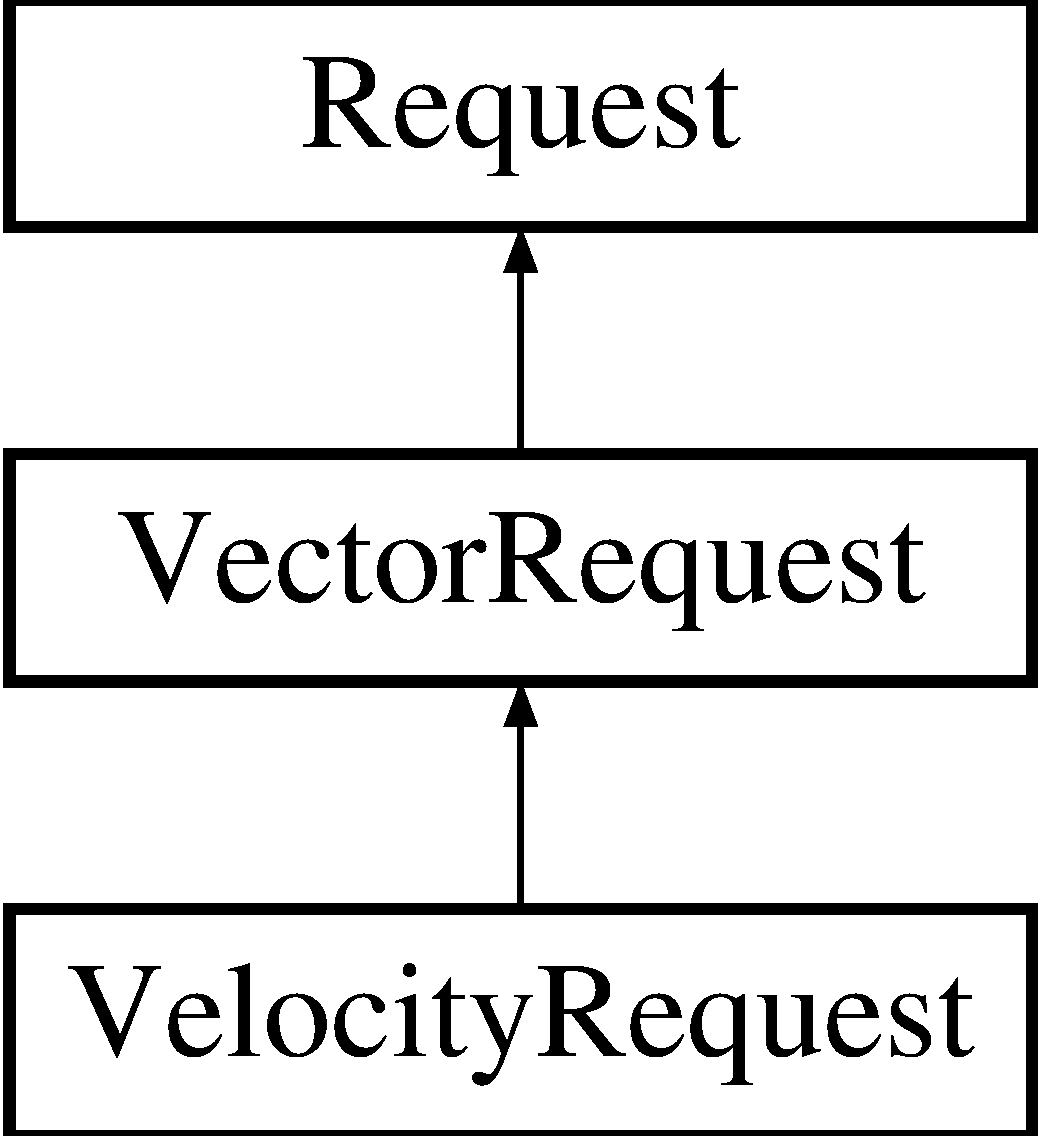
\includegraphics[height=3cm]{class_velocity_request}
\end{center}
\end{figure}
\subsection*{Public Member Functions}
\begin{CompactItemize}
\item 
\hypertarget{class_velocity_request_4d67e0268ad27325e7e06ff5cb9b7d71}{
\textbf{VelocityRequest} (Robot \&robot, boost::shared\_\-ptr$<$ Vector3d $>$ requested\_\-vector)}
\label{class_velocity_request_4d67e0268ad27325e7e06ff5cb9b7d71}

\end{CompactItemize}


\subsection{Detailed Description}
A velocity request is issued by a robot which wants to change its velocity to a new value. 

Notes: The new velocity is expressed in terms of the local coordinate system of the robot. This means it has to be transformed before using.

The request cannot be changed after construction. 

Definition at line 23 of file velocity\_\-request.h.

The documentation for this class was generated from the following file:\begin{CompactItemize}
\item 
src/Requests/velocity\_\-request.h\end{CompactItemize}

\hypertarget{class_view}{
\section{View Class Reference}
\label{class_view}\index{View@{View}}
}
Interface for Robot::compute() to the \hyperlink{class_world_information}{WorldInformation}.  


{\tt \#include $<$view.h$>$}

Inheritance diagram for View::\begin{figure}[H]
\begin{center}
\leavevmode
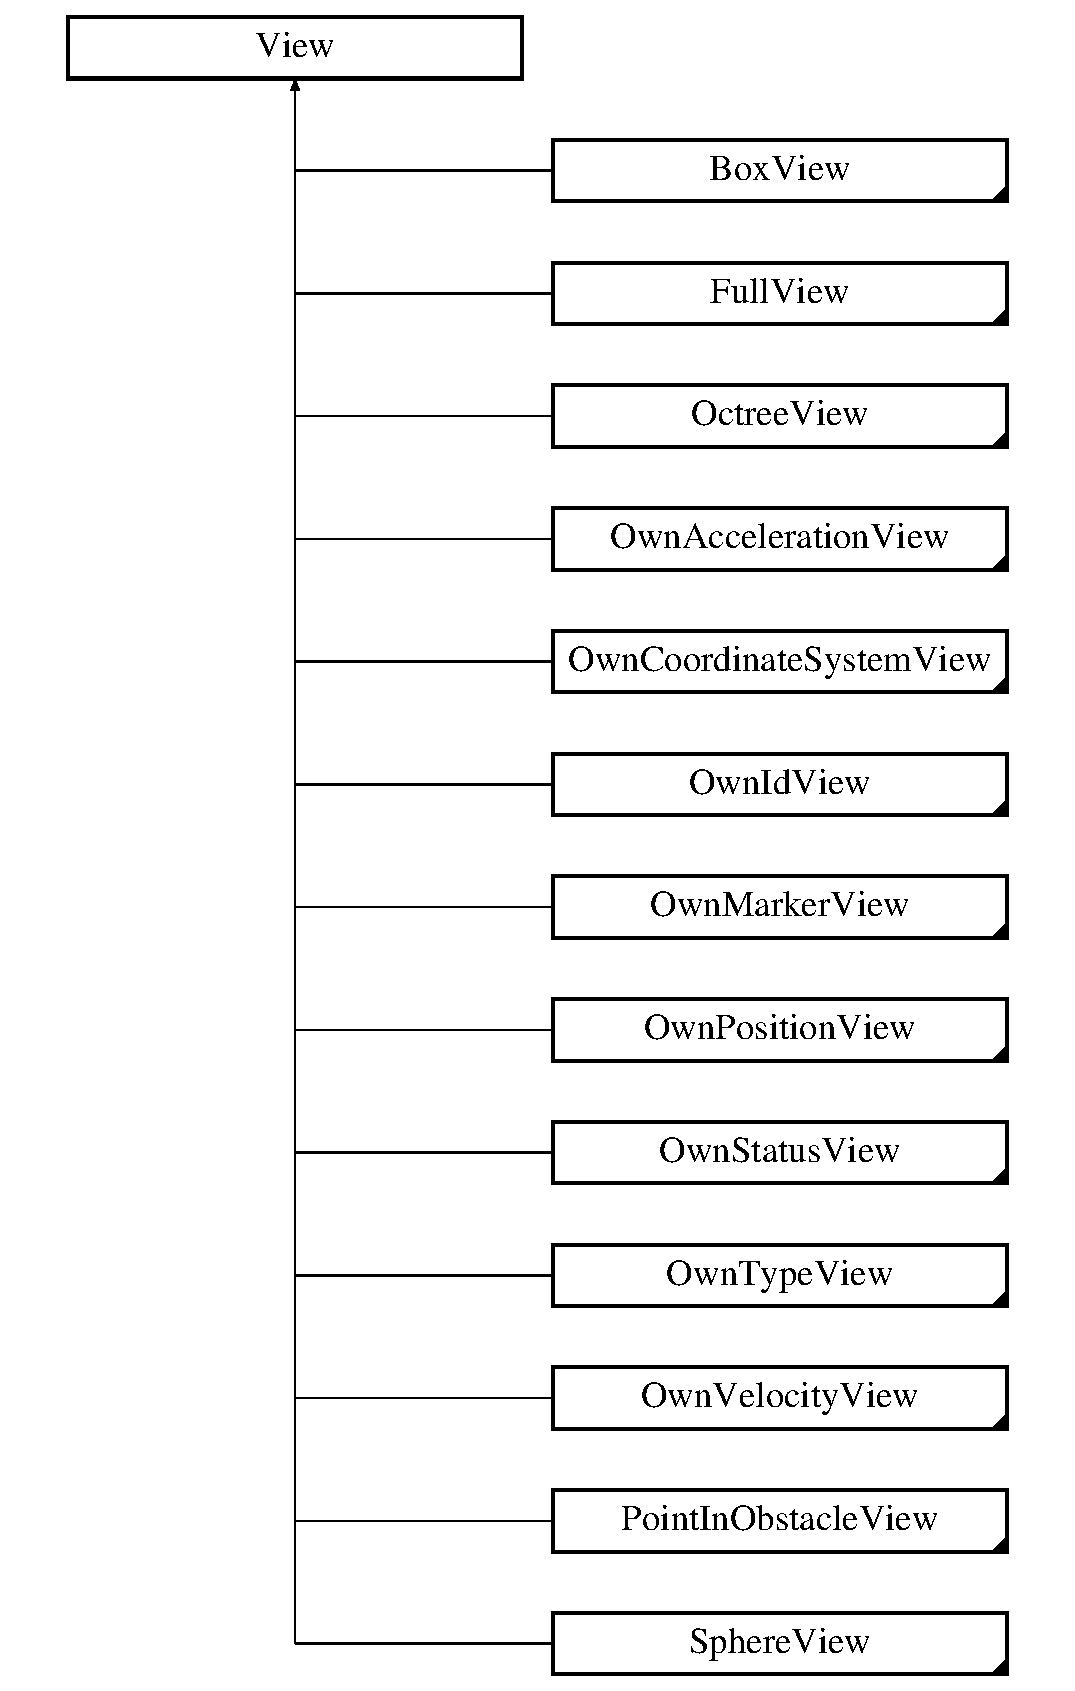
\includegraphics[height=12cm]{class_view}
\end{center}
\end{figure}
\subsection*{Public Member Functions}
\begin{CompactItemize}
\item 
virtual void \hyperlink{class_view_fa489c0530d45e3e24c3151c0908240d}{init} (const \hyperlink{class_world_information}{WorldInformation} \&world\_\-information)
\item 
const std::set$<$ RobotRef $>$ \hyperlink{class_view_10dfd4b4f63f779ca9818317b94aa00b}{get\_\-visible\_\-robots} (const Robot \&caller) const 
\item 
const std::set$<$ ObstacleRef $>$ \hyperlink{class_view_cfc09c1945cd9db211dbd3d202c4393c}{get\_\-visible\_\-obstacles} (const Robot \&caller) const 
\item 
const std::set$<$ MarkerRef $>$ \hyperlink{class_view_6365a5abc73adc91784846713e2d24c6}{get\_\-visible\_\-markers} (const Robot \&caller) const 
\item 
const Vector3d \hyperlink{class_view_58fde47c2b683d13f4d038d3e9b37093}{get\_\-position} (const Robot \&caller, WorldObjectRef world\_\-object) const 
\item 
const \hyperlink{class_marker_information}{MarkerInformation} \hyperlink{class_view_7b23348169617597ddb74988fb3ce3e1}{get\_\-marker\_\-information} (const Robot \&caller, WorldObjectRef world\_\-object) const 
\item 
const std::size\_\-t \hyperlink{class_view_865976d08746c6414ae0068904cf8f9c}{get\_\-id} (const Robot \&caller, WorldObjectRef robot) const 
\item 
const Vector3d \hyperlink{class_view_e1900efc7a61a79882222b9efbcc3708}{get\_\-robot\_\-acceleration} (const Robot \&caller, RobotRef robot) const 
\item 
const boost::tuple$<$ boost::shared\_\-ptr$<$ Vector3d $>$, boost::shared\_\-ptr$<$ Vector3d $>$, boost::shared\_\-ptr$<$ Vector3d $>$ $>$ \hyperlink{class_view_d09f4f177a41f7ea019a08a6dcde3009}{get\_\-robot\_\-coordinate\_\-system\_\-axis} (const Robot \&caller, RobotRef robot) const 
\item 
const RobotType \hyperlink{class_view_ce82208b7d2bf96fbc80d6181c8702cc}{get\_\-robot\_\-type} (const Robot \&caller, RobotRef robot) const 
\item 
const Vector3d \hyperlink{class_view_8fb901f861b3caa776cdd40a8937b929}{get\_\-robot\_\-velocity} (const Robot \&caller, RobotRef robot) const 
\item 
const RobotStatus \hyperlink{class_view_9afafa253b161a72d9d1fa727b652fef}{get\_\-robot\_\-status} (const Robot \&caller, RobotRef robot) const 
\item 
const bool \hyperlink{class_view_4fe93f018f5b3fc812f30e6b0d91c9e6}{is\_\-point\_\-in\_\-obstacle} (ObstacleRef obstacle, const Vector3d \&point) const 
\item 
const double \hyperlink{class_view_87dbec1e6f6add8364f7f73262004088}{get\_\-box\_\-depth} (BoxRef box) const 
\item 
const double \hyperlink{class_view_4dd52be2f5f895efa82622a0e03057f7}{get\_\-box\_\-width} (BoxRef box) const 
\item 
const double \hyperlink{class_view_7b70e3c95c8b45e03230c84b46243cf3}{get\_\-box\_\-height} (BoxRef box) const 
\item 
const double \hyperlink{class_view_b7aa87fa394fbcd9a84e288dd89b36ee}{get\_\-sphere\_\-radius} (SphereRef sphere) const 
\end{CompactItemize}
\subsection*{Protected Types}
\begin{CompactItemize}
\item 
\hypertarget{class_view_680280f66593fcb79cfb5e3f7106870a}{
typedef boost::shared\_\-ptr$<$ \hyperlink{class_robot_identifier}{RobotIdentifier} $>$ \textbf{RobotRef}}
\label{class_view_680280f66593fcb79cfb5e3f7106870a}

\item 
\hypertarget{class_view_b6d68b48711c9c88ac387dab7a0dc522}{
typedef boost::shared\_\-ptr$<$ \hyperlink{class_obstacle_identifier}{ObstacleIdentifier} $>$ \textbf{ObstacleRef}}
\label{class_view_b6d68b48711c9c88ac387dab7a0dc522}

\item 
\hypertarget{class_view_182d3f5872b9dd21a5da8ed81841bec6}{
typedef boost::shared\_\-ptr$<$ \hyperlink{class_box_identifier}{BoxIdentifier} $>$ \textbf{BoxRef}}
\label{class_view_182d3f5872b9dd21a5da8ed81841bec6}

\item 
\hypertarget{class_view_c2a199ef4c72c93c73a5b47fc1de419d}{
typedef boost::shared\_\-ptr$<$ \hyperlink{class_sphere_identifier}{SphereIdentifier} $>$ \textbf{SphereRef}}
\label{class_view_c2a199ef4c72c93c73a5b47fc1de419d}

\item 
\hypertarget{class_view_b697adfcdd10edf1b8b015b1138f3233}{
typedef boost::shared\_\-ptr$<$ \hyperlink{class_marker_identifier}{MarkerIdentifier} $>$ \textbf{MarkerRef}}
\label{class_view_b697adfcdd10edf1b8b015b1138f3233}

\item 
\hypertarget{class_view_e633afa80f7c3c606f0e2b2913726101}{
typedef boost::shared\_\-ptr$<$ \hyperlink{class_identifier}{Identifier} $>$ \textbf{WorldObjectRef}}
\label{class_view_e633afa80f7c3c606f0e2b2913726101}

\end{CompactItemize}
\subsection*{Protected Member Functions}
\begin{CompactItemize}
\item 
\hypertarget{class_view_77f59999d4ea1a733c22c7f28bbc2c0a}{
virtual std::set$<$ RobotRef $>$ \textbf{get\_\-visible\_\-robots} (const \hyperlink{class_robot_data}{RobotData} \&robot) const }
\label{class_view_77f59999d4ea1a733c22c7f28bbc2c0a}

\item 
\hypertarget{class_view_4ee7073dc1981620d21deadaf9f2cc72}{
virtual std::set$<$ ObstacleRef $>$ \textbf{get\_\-visible\_\-obstacles} (const \hyperlink{class_robot_data}{RobotData} \&robot) const }
\label{class_view_4ee7073dc1981620d21deadaf9f2cc72}

\item 
\hypertarget{class_view_6cb28b7cf14724b9583e91f20beab5a7}{
virtual std::set$<$ MarkerRef $>$ \textbf{get\_\-visible\_\-markers} (const \hyperlink{class_robot_data}{RobotData} \&robot) const }
\label{class_view_6cb28b7cf14724b9583e91f20beab5a7}

\item 
\hypertarget{class_view_5d1818431b137cd5d60677060877f9e2}{
virtual Vector3d \textbf{get\_\-own\_\-position} (const \hyperlink{class_robot_data}{RobotData} \&robot) const }
\label{class_view_5d1818431b137cd5d60677060877f9e2}

\item 
\hypertarget{class_view_f2c2e048c57df924cfa28ae4ed0d55f0}{
virtual Vector3d \textbf{get\_\-robot\_\-position} (const \hyperlink{class_robot_data}{RobotData} \&robot) const }
\label{class_view_f2c2e048c57df924cfa28ae4ed0d55f0}

\item 
\hypertarget{class_view_5063b521b3dcf55aa59bbd7061ba63dd}{
virtual Vector3d \textbf{get\_\-obstacle\_\-position} (const Obstacle \&obstacle) const }
\label{class_view_5063b521b3dcf55aa59bbd7061ba63dd}

\item 
\hypertarget{class_view_a1ef1a0dd7bec784ab2648305c832273}{
virtual Vector3d \textbf{get\_\-marker\_\-position} (const \hyperlink{class_world_object}{WorldObject} \&marker) const }
\label{class_view_a1ef1a0dd7bec784ab2648305c832273}

\item 
\hypertarget{class_view_e0b85219f7f81f16c8cff5c62ba5a718}{
virtual \hyperlink{class_marker_information}{MarkerInformation} \textbf{get\_\-own\_\-marker\_\-information} (const \hyperlink{class_robot_data}{RobotData} \&robot) const }
\label{class_view_e0b85219f7f81f16c8cff5c62ba5a718}

\item 
\hypertarget{class_view_38653a1c879f5e6c7c87eff649099a35}{
virtual \hyperlink{class_marker_information}{MarkerInformation} \textbf{get\_\-robots\_\-marker\_\-information} (const \hyperlink{class_robot_data}{RobotData} \&robot) const }
\label{class_view_38653a1c879f5e6c7c87eff649099a35}

\item 
\hypertarget{class_view_fd1b25e5b644b750a7e6b023425115a0}{
virtual \hyperlink{class_marker_information}{MarkerInformation} \textbf{get\_\-obstacles\_\-marker\_\-information} (const Obstacle \&obstacle) const }
\label{class_view_fd1b25e5b644b750a7e6b023425115a0}

\item 
\hypertarget{class_view_86cf2c9c7015f91ee3a065bc2ae65336}{
virtual \hyperlink{class_marker_information}{MarkerInformation} \textbf{get\_\-markers\_\-marker\_\-information} (const \hyperlink{class_world_object}{WorldObject} \&marker) const }
\label{class_view_86cf2c9c7015f91ee3a065bc2ae65336}

\item 
\hypertarget{class_view_b13cfba86985a55f05594e6cb7aa4350}{
virtual std::size\_\-t \textbf{get\_\-own\_\-id} (const \hyperlink{class_robot_data}{RobotData} \&robot) const }
\label{class_view_b13cfba86985a55f05594e6cb7aa4350}

\item 
\hypertarget{class_view_8df1d4d98fa5cb5e02cf7a75d9f92291}{
virtual std::size\_\-t \textbf{get\_\-robot\_\-id} (const \hyperlink{class_robot_data}{RobotData} \&robot) const }
\label{class_view_8df1d4d98fa5cb5e02cf7a75d9f92291}

\item 
\hypertarget{class_view_6b86f8d88388f1da8a03bbf0f158ccbb}{
virtual std::size\_\-t \textbf{get\_\-obstacle\_\-id} (const Obstacle \&obstacle) const }
\label{class_view_6b86f8d88388f1da8a03bbf0f158ccbb}

\item 
\hypertarget{class_view_1ac0779af646011347e44b7e6604d149}{
virtual std::size\_\-t \textbf{get\_\-marker\_\-id} (const \hyperlink{class_world_object}{WorldObject} \&marker) const }
\label{class_view_1ac0779af646011347e44b7e6604d149}

\item 
\hypertarget{class_view_cf225b01ce54de48c6b6617ed14b843a}{
virtual Vector3d \textbf{get\_\-own\_\-acceleration} (const \hyperlink{class_robot_data}{RobotData} \&robot) const }
\label{class_view_cf225b01ce54de48c6b6617ed14b843a}

\item 
\hypertarget{class_view_3e6f92a4b5ea3e4201db27e0e9863f50}{
virtual Vector3d \textbf{get\_\-others\_\-acceleration} (const \hyperlink{class_robot_data}{RobotData} \&robot) const }
\label{class_view_3e6f92a4b5ea3e4201db27e0e9863f50}

\item 
\hypertarget{class_view_c4f04d6595dc1fb83751d17c42ce544c}{
virtual boost::tuple$<$ boost::shared\_\-ptr$<$ Vector3d $>$, boost::shared\_\-ptr$<$ Vector3d $>$, boost::shared\_\-ptr$<$ Vector3d $>$ $>$ \textbf{get\_\-own\_\-coordinate\_\-system\_\-axis} (const \hyperlink{class_robot_data}{RobotData} \&robot) const }
\label{class_view_c4f04d6595dc1fb83751d17c42ce544c}

\item 
\hypertarget{class_view_eed120c2bfefb7202d4402b77d432f8f}{
virtual boost::tuple$<$ boost::shared\_\-ptr$<$ Vector3d $>$, boost::shared\_\-ptr$<$ Vector3d $>$, boost::shared\_\-ptr$<$ Vector3d $>$ $>$ \textbf{get\_\-others\_\-coordinate\_\-system\_\-axis} (const \hyperlink{class_robot_data}{RobotData} \&robot) const }
\label{class_view_eed120c2bfefb7202d4402b77d432f8f}

\item 
\hypertarget{class_view_580b47540374e46099fa73515a372571}{
virtual RobotType \textbf{get\_\-own\_\-type} (const \hyperlink{class_robot_data}{RobotData} \&robot) const }
\label{class_view_580b47540374e46099fa73515a372571}

\item 
\hypertarget{class_view_37ed113fedcce3a5589ac088b70551d4}{
virtual RobotType \textbf{get\_\-others\_\-type} (const \hyperlink{class_robot_data}{RobotData} \&robot) const }
\label{class_view_37ed113fedcce3a5589ac088b70551d4}

\item 
\hypertarget{class_view_ce6be029d20d03891468aca61961e6d5}{
virtual Vector3d \textbf{get\_\-own\_\-velocity} (const \hyperlink{class_robot_data}{RobotData} \&robot) const }
\label{class_view_ce6be029d20d03891468aca61961e6d5}

\item 
\hypertarget{class_view_6d4aca6107649cb75a133745e860f8e3}{
virtual Vector3d \textbf{get\_\-others\_\-velocity} (const \hyperlink{class_robot_data}{RobotData} \&robot) const }
\label{class_view_6d4aca6107649cb75a133745e860f8e3}

\item 
\hypertarget{class_view_8dfd78e2f19f9bb1a6cdafcebb28b78e}{
virtual RobotStatus \textbf{get\_\-own\_\-status} (const \hyperlink{class_robot_data}{RobotData} \&robot) const }
\label{class_view_8dfd78e2f19f9bb1a6cdafcebb28b78e}

\item 
\hypertarget{class_view_92957bbd0b1b435457aaa1929d2624e7}{
virtual RobotStatus \textbf{get\_\-others\_\-status} (const \hyperlink{class_robot_data}{RobotData} \&robot) const }
\label{class_view_92957bbd0b1b435457aaa1929d2624e7}

\item 
\hypertarget{class_view_a74a9578c6666c81a68c28e820a79afc}{
virtual bool \textbf{is\_\-point\_\-in\_\-obstacle} (const Obstacle \&obstacle, const Vector3d \&point) const }
\label{class_view_a74a9578c6666c81a68c28e820a79afc}

\item 
\hypertarget{class_view_0b6fb511a898ac846f3cccfe8fa001be}{
virtual double \textbf{get\_\-box\_\-depth} (const \hyperlink{class_box}{Box} \&box) const }
\label{class_view_0b6fb511a898ac846f3cccfe8fa001be}

\item 
\hypertarget{class_view_9c80969a2b1c7d666f69c3f231497b38}{
virtual double \textbf{get\_\-box\_\-width} (const \hyperlink{class_box}{Box} \&box) const }
\label{class_view_9c80969a2b1c7d666f69c3f231497b38}

\item 
\hypertarget{class_view_cf48aefe3cd585a6ffb006b35335b77d}{
virtual double \textbf{get\_\-box\_\-height} (const \hyperlink{class_box}{Box} \&box) const }
\label{class_view_cf48aefe3cd585a6ffb006b35335b77d}

\item 
\hypertarget{class_view_e0d7ac1ffcaced2ad17fd0523ae22132}{
virtual double \textbf{get\_\-sphere\_\-radius} (const \hyperlink{class_sphere}{Sphere} \&sphere) const }
\label{class_view_e0d7ac1ffcaced2ad17fd0523ae22132}

\item 
\hypertarget{class_view_0d4525686368867a77c6e96d8844b6eb}{
const \hyperlink{class_world_information}{WorldInformation} \& \textbf{world\_\-information} () const }
\label{class_view_0d4525686368867a77c6e96d8844b6eb}

\item 
\hypertarget{class_view_40880e5f3127deec2540235a657c749e}{
const std::size\_\-t \textbf{get\_\-id} (boost::shared\_\-ptr$<$ \hyperlink{class_identifier}{Identifier} $>$ identifier) const }
\label{class_view_40880e5f3127deec2540235a657c749e}

\end{CompactItemize}
\subsection*{Private Member Functions}
\begin{CompactItemize}
\item 
\hypertarget{class_view_26da087403dfa4e35dcb782209e5b452}{
const Obstacle \& \textbf{resolve\_\-obstacle\_\-ref} (ObstacleRef obstacle) const }
\label{class_view_26da087403dfa4e35dcb782209e5b452}

\item 
\hypertarget{class_view_ea0e2f72b7d61e193b8535ffbd31a55a}{
const \hyperlink{class_robot_data}{RobotData} \& \textbf{resolve\_\-robot\_\-ref} (RobotRef robot) const }
\label{class_view_ea0e2f72b7d61e193b8535ffbd31a55a}

\item 
\hypertarget{class_view_d4baccf339e1f80a5ea51c38fd43a1ca}{
const \hyperlink{class_world_object}{WorldObject} \& \textbf{resolve\_\-marker\_\-ref} (MarkerRef marker) const }
\label{class_view_d4baccf339e1f80a5ea51c38fd43a1ca}

\item 
\hypertarget{class_view_c36b06dfedbf8e0b411f0e9f411bca9e}{
const \hyperlink{class_box}{Box} \& \textbf{resolve\_\-box\_\-ref} (BoxRef box) const }
\label{class_view_c36b06dfedbf8e0b411f0e9f411bca9e}

\item 
\hypertarget{class_view_4b2586808a208a032133826f6d958765}{
const \hyperlink{class_sphere}{Sphere} \& \textbf{resolve\_\-sphere\_\-ref} (SphereRef sphere) const }
\label{class_view_4b2586808a208a032133826f6d958765}

\item 
\hypertarget{class_view_59d1a4d60b56c682fd791e89d65ce6bb}{
const Obstacle \& \textbf{resolve\_\-obstacle\_\-ref\_\-safe} (ObstacleRef obstacle) const }
\label{class_view_59d1a4d60b56c682fd791e89d65ce6bb}

\item 
\hypertarget{class_view_82439df63b460f9d1eb098b3f5bcba4f}{
const \hyperlink{class_robot_data}{RobotData} \& \textbf{resolve\_\-robot\_\-ref\_\-safe} (RobotRef robot) const }
\label{class_view_82439df63b460f9d1eb098b3f5bcba4f}

\item 
\hypertarget{class_view_6fe4251a36f7df350f312fd19033812c}{
const \hyperlink{class_world_object}{WorldObject} \& \textbf{resolve\_\-marker\_\-ref\_\-safe} (MarkerRef marker) const }
\label{class_view_6fe4251a36f7df350f312fd19033812c}

\item 
\hypertarget{class_view_b641c6d8d9595721f0d43931da47c2d2}{
const \hyperlink{class_box}{Box} \& \textbf{resolve\_\-box\_\-ref\_\-safe} (BoxRef box) const }
\label{class_view_b641c6d8d9595721f0d43931da47c2d2}

\item 
\hypertarget{class_view_66c7a54d9f85ced79c33f3b17f34f4bf}{
const \hyperlink{class_sphere}{Sphere} \& \textbf{resolve\_\-sphere\_\-ref\_\-safe} (SphereRef sphere) const }
\label{class_view_66c7a54d9f85ced79c33f3b17f34f4bf}

\item 
{\footnotesize template$<$typename T$>$ }\\T \hyperlink{class_view_7eccca274db6bd4da79a294e463de06c}{delegate\_\-function} (boost::function$<$ T(const \hyperlink{class_view}{View} $\ast$, const \hyperlink{class_robot_data}{RobotData} \&)$>$ own\_\-robot\_\-fun, boost::function$<$ T(const \hyperlink{class_view}{View} $\ast$, const \hyperlink{class_robot_data}{RobotData} \&)$>$ other\_\-robot\_\-fun, boost::function$<$ T(const \hyperlink{class_view}{View} $\ast$, const Obstacle \&)$>$ obstacle\_\-fun, boost::function$<$ T(const \hyperlink{class_view}{View} $\ast$, const \hyperlink{class_world_object}{WorldObject} \&)$>$ marker\_\-fun, const Robot \&caller, WorldObjectRef world\_\-object) const 
\item 
{\footnotesize template$<$typename T$>$ }\\T \hyperlink{class_view_9fce14f4a6491176e28f19d41669a136}{delegate\_\-function} (boost::function$<$ T(const \hyperlink{class_view}{View} $\ast$, const \hyperlink{class_robot_data}{RobotData} \&)$>$ own\_\-robot\_\-fun, boost::function$<$ T(const \hyperlink{class_view}{View} $\ast$, const \hyperlink{class_robot_data}{RobotData} \&)$>$ other\_\-robot\_\-fun, const Robot \&caller, RobotRef robot) const 
\end{CompactItemize}
\subsection*{Static Private Member Functions}
\begin{CompactItemize}
\item 
static bool \hyperlink{class_view_72674a687dbcec3e4a58191a65fd1ace}{is\_\-own\_\-identifier} (const Robot \&robot, boost::shared\_\-ptr$<$ \hyperlink{class_robot_identifier}{RobotIdentifier} $>$ identifier)
\end{CompactItemize}
\subsection*{Private Attributes}
\begin{CompactItemize}
\item 
\hypertarget{class_view_cab113a8a94e62a8dc1ed7b09d98bed3}{
const \hyperlink{class_world_information}{WorldInformation} $\ast$ \textbf{world\_\-information\_\-}}
\label{class_view_cab113a8a94e62a8dc1ed7b09d98bed3}

\end{CompactItemize}


\subsection{Detailed Description}
Interface for Robot::compute() to the \hyperlink{class_world_information}{WorldInformation}. 

The \hyperlink{class_view}{View} class represents the robots view to the world, i.e. a \hyperlink{class_view}{View} class describes the information model that should be used for this simulation. This class is designed as a base class for more concrete models. Still there are no abstract methods. Instead, all methods are implemented such, that they throw a NotSupportedOperationException.

Note: Most methods specified in this class need to know the calling Robot, so they determine whether e.g. the own position is queried or the position of an other Robot.

Assigning this class to a Robot corresponds to a \char`\"{}no information at all\char`\"{} model for each Robot. 

Definition at line 47 of file view.h.

\subsection{Member Function Documentation}
\hypertarget{class_view_fa489c0530d45e3e24c3151c0908240d}{
\index{View@{View}!init@{init}}
\index{init@{init}!View@{View}}
\subsubsection[init]{\setlength{\rightskip}{0pt plus 5cm}void View::init (const {\bf WorldInformation} \& {\em world\_\-information})\hspace{0.3cm}{\tt  \mbox{[}virtual\mbox{]}}}}
\label{class_view_fa489c0530d45e3e24c3151c0908240d}


Although init is trivial, it is nice to have a default constructor in virtual inherited classes. Otherwise every arbitrary deep sub class has to call the non-default constructor. Call this method before using any other method of \hyperlink{class_view}{View}. \begin{Desc}
\item[Parameters:]
\begin{description}
\item[{\em \hyperlink{class_world_information}{WorldInformation}}]\end{description}
\end{Desc}


Reimplemented in \hyperlink{class_octree_view_800b8d09dbd898769439f1765e7d87b1}{OctreeView}, and \hyperlink{class_spheric_view_dbd6a1d5e2f17594f82e831c38d35ec6}{SphericView}.

Definition at line 118 of file view.cc.

Referenced by SphericView::init(), and OctreeView::init().\hypertarget{class_view_10dfd4b4f63f779ca9818317b94aa00b}{
\index{View@{View}!get\_\-visible\_\-robots@{get\_\-visible\_\-robots}}
\index{get\_\-visible\_\-robots@{get\_\-visible\_\-robots}!View@{View}}
\subsubsection[get\_\-visible\_\-robots]{\setlength{\rightskip}{0pt plus 5cm}const std::set$<$ View::RobotRef $>$ View::get\_\-visible\_\-robots (const Robot \& {\em caller}) const}}
\label{class_view_10dfd4b4f63f779ca9818317b94aa00b}


Returns the set of robots visible for the calling Robot. Note: The \hyperlink{class_identifier}{Identifier} of the calling Robot is never returned by this method. \begin{Desc}
\item[Parameters:]
\begin{description}
\item[{\em Robot}]that should take a look-around \end{description}
\end{Desc}
\begin{Desc}
\item[Returns:]set of robots visible \end{Desc}


Definition at line 123 of file view.cc.\hypertarget{class_view_cfc09c1945cd9db211dbd3d202c4393c}{
\index{View@{View}!get\_\-visible\_\-obstacles@{get\_\-visible\_\-obstacles}}
\index{get\_\-visible\_\-obstacles@{get\_\-visible\_\-obstacles}!View@{View}}
\subsubsection[get\_\-visible\_\-obstacles]{\setlength{\rightskip}{0pt plus 5cm}const std::set$<$ View::ObstacleRef $>$ View::get\_\-visible\_\-obstacles (const Robot \& {\em caller}) const}}
\label{class_view_cfc09c1945cd9db211dbd3d202c4393c}


Returns the set of obstacles visible for the calling Robot. \begin{Desc}
\item[Parameters:]
\begin{description}
\item[{\em Robot}]that should take a look-around \end{description}
\end{Desc}
\begin{Desc}
\item[Returns:]set of obstacles visible \end{Desc}


Definition at line 129 of file view.cc.\hypertarget{class_view_6365a5abc73adc91784846713e2d24c6}{
\index{View@{View}!get\_\-visible\_\-markers@{get\_\-visible\_\-markers}}
\index{get\_\-visible\_\-markers@{get\_\-visible\_\-markers}!View@{View}}
\subsubsection[get\_\-visible\_\-markers]{\setlength{\rightskip}{0pt plus 5cm}const std::set$<$ View::MarkerRef $>$ View::get\_\-visible\_\-markers (const Robot \& {\em caller}) const}}
\label{class_view_6365a5abc73adc91784846713e2d24c6}


Returns the set of markers visible for the calling Robot. \begin{Desc}
\item[Parameters:]
\begin{description}
\item[{\em Robot}]that should take a look-around \end{description}
\end{Desc}
\begin{Desc}
\item[Returns:]set of markers visible \end{Desc}


Definition at line 135 of file view.cc.\hypertarget{class_view_58fde47c2b683d13f4d038d3e9b37093}{
\index{View@{View}!get\_\-position@{get\_\-position}}
\index{get\_\-position@{get\_\-position}!View@{View}}
\subsubsection[get\_\-position]{\setlength{\rightskip}{0pt plus 5cm}const Vector3d View::get\_\-position (const Robot \& {\em caller}, \/  WorldObjectRef {\em world\_\-object}) const}}
\label{class_view_58fde47c2b683d13f4d038d3e9b37093}


Queries for the position of a \hyperlink{class_world_object}{WorldObject} identified by an given \hyperlink{class_identifier}{Identifier}. \begin{Desc}
\item[Parameters:]
\begin{description}
\item[{\em The}]Robot which is asking.. \item[{\em \hyperlink{class_identifier}{Identifier}}]for a \hyperlink{class_world_object}{WorldObject} \end{description}
\end{Desc}
\begin{Desc}
\item[Returns:]Position \end{Desc}
\begin{Desc}
\item[See also:]\hyperlink{class_world_object_27b52dcd1b64d4dd45936da833e1ea26}{WorldObject::position()} \end{Desc}


Definition at line 140 of file view.cc.

References CoordConverter::global\_\-to\_\-local().\hypertarget{class_view_7b23348169617597ddb74988fb3ce3e1}{
\index{View@{View}!get\_\-marker\_\-information@{get\_\-marker\_\-information}}
\index{get\_\-marker\_\-information@{get\_\-marker\_\-information}!View@{View}}
\subsubsection[get\_\-marker\_\-information]{\setlength{\rightskip}{0pt plus 5cm}const {\bf MarkerInformation} View::get\_\-marker\_\-information (const Robot \& {\em caller}, \/  WorldObjectRef {\em world\_\-object}) const}}
\label{class_view_7b23348169617597ddb74988fb3ce3e1}


Queries for the marker information of a \hyperlink{class_world_object}{WorldObject} identified by an given \hyperlink{class_identifier}{Identifier}. \begin{Desc}
\item[Parameters:]
\begin{description}
\item[{\em The}]Robot which is asking.. \item[{\em \hyperlink{class_identifier}{Identifier}}]for a \hyperlink{class_world_object}{WorldObject} \end{description}
\end{Desc}
\begin{Desc}
\item[Returns:]\hyperlink{class_marker_information}{MarkerInformation} \end{Desc}
\begin{Desc}
\item[See also:]\hyperlink{class_world_object_1dd7d80498c6b502ad9870c54cbf4305}{WorldObject::marker\_\-information()} \end{Desc}


Definition at line 149 of file view.cc.\hypertarget{class_view_865976d08746c6414ae0068904cf8f9c}{
\index{View@{View}!get\_\-id@{get\_\-id}}
\index{get\_\-id@{get\_\-id}!View@{View}}
\subsubsection[get\_\-id]{\setlength{\rightskip}{0pt plus 5cm}const std::size\_\-t View::get\_\-id (const Robot \& {\em caller}, \/  WorldObjectRef {\em robot}) const}}
\label{class_view_865976d08746c6414ae0068904cf8f9c}


Queries for the id of a WordObject identified by an given \hyperlink{class_identifier}{Identifier}. \begin{Desc}
\item[Parameters:]
\begin{description}
\item[{\em The}]Robot which is asking.. \item[{\em \hyperlink{class_identifier}{Identifier}}]for a \hyperlink{class_world_object}{WorldObject} \end{description}
\end{Desc}
\begin{Desc}
\item[Returns:]id \end{Desc}
\begin{Desc}
\item[See also:]\hyperlink{class_world_object_86cb6d16f21d52ebe8f9dc48e9e762f3}{WorldObject::id()} \end{Desc}


Definition at line 155 of file view.cc.\hypertarget{class_view_e1900efc7a61a79882222b9efbcc3708}{
\index{View@{View}!get\_\-robot\_\-acceleration@{get\_\-robot\_\-acceleration}}
\index{get\_\-robot\_\-acceleration@{get\_\-robot\_\-acceleration}!View@{View}}
\subsubsection[get\_\-robot\_\-acceleration]{\setlength{\rightskip}{0pt plus 5cm}const Vector3d View::get\_\-robot\_\-acceleration (const Robot \& {\em caller}, \/  RobotRef {\em robot}) const}}
\label{class_view_e1900efc7a61a79882222b9efbcc3708}


Queries for the acceleration of a Robot identified by an given \hyperlink{class_robot_identifier}{RobotIdentifier}. \begin{Desc}
\item[Parameters:]
\begin{description}
\item[{\em The}]Robot which is asking.. \item[{\em \hyperlink{class_robot_identifier}{RobotIdentifier}}]\end{description}
\end{Desc}
\begin{Desc}
\item[Returns:]Vector3d \end{Desc}
\begin{Desc}
\item[See also:]\hyperlink{class_robot_data_a65f6448e4ec4061b6300283f3cdd8da}{RobotData::acceleration()} \end{Desc}


Definition at line 161 of file view.cc.\hypertarget{class_view_d09f4f177a41f7ea019a08a6dcde3009}{
\index{View@{View}!get\_\-robot\_\-coordinate\_\-system\_\-axis@{get\_\-robot\_\-coordinate\_\-system\_\-axis}}
\index{get\_\-robot\_\-coordinate\_\-system\_\-axis@{get\_\-robot\_\-coordinate\_\-system\_\-axis}!View@{View}}
\subsubsection[get\_\-robot\_\-coordinate\_\-system\_\-axis]{\setlength{\rightskip}{0pt plus 5cm}const boost::tuple$<$ boost::shared\_\-ptr$<$ Vector3d $>$, boost::shared\_\-ptr$<$ Vector3d $>$, boost::shared\_\-ptr$<$ Vector3d $>$ $>$ View::get\_\-robot\_\-coordinate\_\-system\_\-axis (const Robot \& {\em caller}, \/  RobotRef {\em robot}) const}}
\label{class_view_d09f4f177a41f7ea019a08a6dcde3009}


Queries for the coordinate system axes of a Robot identified by an given \hyperlink{class_robot_identifier}{RobotIdentifier}. \begin{Desc}
\item[Parameters:]
\begin{description}
\item[{\em The}]Robot which is asking.. \item[{\em \hyperlink{class_robot_identifier}{RobotIdentifier}}]\end{description}
\end{Desc}
\begin{Desc}
\item[Returns:]Vector3d \end{Desc}
\begin{Desc}
\item[See also:]\hyperlink{class_robot_data_e093fc063e47ad844c20a9332c5bea6a}{RobotData::coordinate\_\-system\_\-axis()} \end{Desc}


Definition at line 165 of file view.cc.\hypertarget{class_view_ce82208b7d2bf96fbc80d6181c8702cc}{
\index{View@{View}!get\_\-robot\_\-type@{get\_\-robot\_\-type}}
\index{get\_\-robot\_\-type@{get\_\-robot\_\-type}!View@{View}}
\subsubsection[get\_\-robot\_\-type]{\setlength{\rightskip}{0pt plus 5cm}const RobotType View::get\_\-robot\_\-type (const Robot \& {\em caller}, \/  RobotRef {\em robot}) const}}
\label{class_view_ce82208b7d2bf96fbc80d6181c8702cc}


Queries for the robot type of a Robot identified by an given \hyperlink{class_robot_identifier}{RobotIdentifier}. \begin{Desc}
\item[Parameters:]
\begin{description}
\item[{\em The}]Robot which is asking.. \item[{\em \hyperlink{class_robot_identifier}{RobotIdentifier}}]\end{description}
\end{Desc}
\begin{Desc}
\item[Returns:]RobotType \end{Desc}
\begin{Desc}
\item[See also:]\hyperlink{class_robot_data_b83255012ce788fdbf9b277c775e0240}{RobotData::type()} \end{Desc}


Definition at line 171 of file view.cc.\hypertarget{class_view_8fb901f861b3caa776cdd40a8937b929}{
\index{View@{View}!get\_\-robot\_\-velocity@{get\_\-robot\_\-velocity}}
\index{get\_\-robot\_\-velocity@{get\_\-robot\_\-velocity}!View@{View}}
\subsubsection[get\_\-robot\_\-velocity]{\setlength{\rightskip}{0pt plus 5cm}const Vector3d View::get\_\-robot\_\-velocity (const Robot \& {\em caller}, \/  RobotRef {\em robot}) const}}
\label{class_view_8fb901f861b3caa776cdd40a8937b929}


Queries for the velocity of a Robot identified by an given \hyperlink{class_robot_identifier}{RobotIdentifier}. \begin{Desc}
\item[Parameters:]
\begin{description}
\item[{\em The}]Robot which is asking.. \item[{\em \hyperlink{class_robot_identifier}{RobotIdentifier}}]\end{description}
\end{Desc}
\begin{Desc}
\item[Returns:]Vector3d \end{Desc}
\begin{Desc}
\item[See also:]\hyperlink{class_robot_data_933da54224245d40afb0ed1b2446599c}{RobotData::velocity()} \end{Desc}


Definition at line 175 of file view.cc.\hypertarget{class_view_9afafa253b161a72d9d1fa727b652fef}{
\index{View@{View}!get\_\-robot\_\-status@{get\_\-robot\_\-status}}
\index{get\_\-robot\_\-status@{get\_\-robot\_\-status}!View@{View}}
\subsubsection[get\_\-robot\_\-status]{\setlength{\rightskip}{0pt plus 5cm}const RobotStatus View::get\_\-robot\_\-status (const Robot \& {\em caller}, \/  RobotRef {\em robot}) const}}
\label{class_view_9afafa253b161a72d9d1fa727b652fef}


Queries for the status of a Robot identified by an given \hyperlink{class_robot_identifier}{RobotIdentifier}. \begin{Desc}
\item[Parameters:]
\begin{description}
\item[{\em The}]Robot which is asking.. \item[{\em \hyperlink{class_robot_identifier}{RobotIdentifier}}]\end{description}
\end{Desc}
\begin{Desc}
\item[Returns:]RobotStatus \end{Desc}
\begin{Desc}
\item[See also:]\hyperlink{class_robot_data_9c8d2252555f1d5866c0332a80e82685}{RobotData::status()} \end{Desc}


Definition at line 179 of file view.cc.\hypertarget{class_view_4fe93f018f5b3fc812f30e6b0d91c9e6}{
\index{View@{View}!is\_\-point\_\-in\_\-obstacle@{is\_\-point\_\-in\_\-obstacle}}
\index{is\_\-point\_\-in\_\-obstacle@{is\_\-point\_\-in\_\-obstacle}!View@{View}}
\subsubsection[is\_\-point\_\-in\_\-obstacle]{\setlength{\rightskip}{0pt plus 5cm}const bool View::is\_\-point\_\-in\_\-obstacle (ObstacleRef {\em obstacle}, \/  const Vector3d \& {\em point}) const}}
\label{class_view_4fe93f018f5b3fc812f30e6b0d91c9e6}


Checks for a given point whether it is contained in a Obstacle identified by a given \hyperlink{class_obstacle_identifier}{ObstacleIdentifier}. \begin{Desc}
\item[Parameters:]
\begin{description}
\item[{\em \hyperlink{class_obstacle_identifier}{ObstacleIdentifier}}]\item[{\em point}]\end{description}
\end{Desc}
\begin{Desc}
\item[Returns:]true if point is contained in the obstacle; false, otherwise \end{Desc}
\begin{Desc}
\item[See also:]Obstacle::contains\_\-point() \end{Desc}


Definition at line 183 of file view.cc.\hypertarget{class_view_87dbec1e6f6add8364f7f73262004088}{
\index{View@{View}!get\_\-box\_\-depth@{get\_\-box\_\-depth}}
\index{get\_\-box\_\-depth@{get\_\-box\_\-depth}!View@{View}}
\subsubsection[get\_\-box\_\-depth]{\setlength{\rightskip}{0pt plus 5cm}const double View::get\_\-box\_\-depth (BoxRef {\em box}) const}}
\label{class_view_87dbec1e6f6add8364f7f73262004088}


Queries for the depth of a \hyperlink{class_box}{Box} identified by an given \hyperlink{class_box_identifier}{BoxIdentifier}. \begin{Desc}
\item[Parameters:]
\begin{description}
\item[{\em \hyperlink{class_box_identifier}{BoxIdentifier}}]\end{description}
\end{Desc}
\begin{Desc}
\item[Returns:]depth \end{Desc}
\begin{Desc}
\item[See also:]\hyperlink{class_box_10dbd2cb5f3c37ca36792d4a1e34240d}{Box::depth()} \end{Desc}


Definition at line 187 of file view.cc.\hypertarget{class_view_4dd52be2f5f895efa82622a0e03057f7}{
\index{View@{View}!get\_\-box\_\-width@{get\_\-box\_\-width}}
\index{get\_\-box\_\-width@{get\_\-box\_\-width}!View@{View}}
\subsubsection[get\_\-box\_\-width]{\setlength{\rightskip}{0pt plus 5cm}const double View::get\_\-box\_\-width (BoxRef {\em box}) const}}
\label{class_view_4dd52be2f5f895efa82622a0e03057f7}


Queries for the width of a \hyperlink{class_box}{Box} identified by an given \hyperlink{class_box_identifier}{BoxIdentifier}. \begin{Desc}
\item[Parameters:]
\begin{description}
\item[{\em \hyperlink{class_box_identifier}{BoxIdentifier}}]\end{description}
\end{Desc}
\begin{Desc}
\item[Returns:]width \end{Desc}
\begin{Desc}
\item[See also:]\hyperlink{class_box_cceec88bdb7cccd65b090837e919982c}{Box::width()} \end{Desc}


Definition at line 191 of file view.cc.\hypertarget{class_view_7b70e3c95c8b45e03230c84b46243cf3}{
\index{View@{View}!get\_\-box\_\-height@{get\_\-box\_\-height}}
\index{get\_\-box\_\-height@{get\_\-box\_\-height}!View@{View}}
\subsubsection[get\_\-box\_\-height]{\setlength{\rightskip}{0pt plus 5cm}const double View::get\_\-box\_\-height (BoxRef {\em box}) const}}
\label{class_view_7b70e3c95c8b45e03230c84b46243cf3}


Queries for the height of a \hyperlink{class_box}{Box} identified by an given \hyperlink{class_box_identifier}{BoxIdentifier}. \begin{Desc}
\item[Parameters:]
\begin{description}
\item[{\em \hyperlink{class_box_identifier}{BoxIdentifier}}]\end{description}
\end{Desc}
\begin{Desc}
\item[Returns:]height \end{Desc}
\begin{Desc}
\item[See also:]\hyperlink{class_box_8b436da1c22ee2335d692fe44c53ce90}{Box::height()} \end{Desc}


Definition at line 195 of file view.cc.\hypertarget{class_view_b7aa87fa394fbcd9a84e288dd89b36ee}{
\index{View@{View}!get\_\-sphere\_\-radius@{get\_\-sphere\_\-radius}}
\index{get\_\-sphere\_\-radius@{get\_\-sphere\_\-radius}!View@{View}}
\subsubsection[get\_\-sphere\_\-radius]{\setlength{\rightskip}{0pt plus 5cm}const double View::get\_\-sphere\_\-radius (SphereRef {\em sphere}) const}}
\label{class_view_b7aa87fa394fbcd9a84e288dd89b36ee}


Queries for the radius of a \hyperlink{class_sphere}{Sphere} identified by an given \hyperlink{class_sphere_identifier}{SphereIdentifier}. \begin{Desc}
\item[Parameters:]
\begin{description}
\item[{\em \hyperlink{class_sphere_identifier}{SphereIdentifier}}]\end{description}
\end{Desc}
\begin{Desc}
\item[Returns:]radius \end{Desc}
\begin{Desc}
\item[See also:]\hyperlink{class_sphere_82c3e6746f79196c744b46f39569689e}{Sphere::radius()} \end{Desc}


Definition at line 199 of file view.cc.\hypertarget{class_view_72674a687dbcec3e4a58191a65fd1ace}{
\index{View@{View}!is\_\-own\_\-identifier@{is\_\-own\_\-identifier}}
\index{is\_\-own\_\-identifier@{is\_\-own\_\-identifier}!View@{View}}
\subsubsection[is\_\-own\_\-identifier]{\setlength{\rightskip}{0pt plus 5cm}bool View::is\_\-own\_\-identifier (const Robot \& {\em robot}, \/  boost::shared\_\-ptr$<$ {\bf RobotIdentifier} $>$ {\em identifier})\hspace{0.3cm}{\tt  \mbox{[}static, private\mbox{]}}}}
\label{class_view_72674a687dbcec3e4a58191a65fd1ace}


Helper methods to check if the given \hyperlink{class_identifier}{Identifier} points to the same data object as the given Robots \hyperlink{class_identifier}{Identifier} does. To do so it compares the internal id of the Identifiers. (Thats also why this method is defined as class method (needs friend access)). 

Definition at line 72 of file view.cc.

Referenced by delegate\_\-function().\hypertarget{class_view_7eccca274db6bd4da79a294e463de06c}{
\index{View@{View}!delegate\_\-function@{delegate\_\-function}}
\index{delegate\_\-function@{delegate\_\-function}!View@{View}}
\subsubsection[delegate\_\-function]{\setlength{\rightskip}{0pt plus 5cm}template$<$typename T$>$ T View::delegate\_\-function (boost::function$<$ T(const {\bf View} $\ast$, const {\bf RobotData} \&)$>$ {\em own\_\-robot\_\-fun}, \/  boost::function$<$ T(const {\bf View} $\ast$, const {\bf RobotData} \&)$>$ {\em other\_\-robot\_\-fun}, \/  boost::function$<$ T(const {\bf View} $\ast$, const Obstacle \&)$>$ {\em obstacle\_\-fun}, \/  boost::function$<$ T(const {\bf View} $\ast$, const {\bf WorldObject} \&)$>$ {\em marker\_\-fun}, \/  const Robot \& {\em caller}, \/  WorldObjectRef {\em world\_\-object}) const\hspace{0.3cm}{\tt  \mbox{[}inline, private\mbox{]}}}}
\label{class_view_7eccca274db6bd4da79a294e463de06c}


Given a set of four methods this method decides which to call. This is used by \hyperlink{class_view_58fde47c2b683d13f4d038d3e9b37093}{View::get\_\-position} for example to delegate the call the View::get\_\-own\_\-position, View::get\_\-robot\_\-position, View::get\_\-obstacle\_\-position, and View::get\_\-marker\_\-position. Which method is called is decided as in View::get\_\-own\_\-position described.

The method uses resolve\_\-$\ast$\_\-ref\_\-safe to resolve arguments for the given methods. A notable exception is the own\_\-robot\_\-function where resolve\_\-robot\_\-ref is used instead. This is because \hyperlink{class_identifier}{Identifier} saved in Robot need not be same as saved in \hyperlink{class_robot_data}{RobotData} (pointerwise). 

Definition at line 41 of file view.cc.

References is\_\-own\_\-identifier().\hypertarget{class_view_9fce14f4a6491176e28f19d41669a136}{
\index{View@{View}!delegate\_\-function@{delegate\_\-function}}
\index{delegate\_\-function@{delegate\_\-function}!View@{View}}
\subsubsection[delegate\_\-function]{\setlength{\rightskip}{0pt plus 5cm}template$<$typename T$>$ T View::delegate\_\-function (boost::function$<$ T(const {\bf View} $\ast$, const {\bf RobotData} \&)$>$ {\em own\_\-robot\_\-fun}, \/  boost::function$<$ T(const {\bf View} $\ast$, const {\bf RobotData} \&)$>$ {\em other\_\-robot\_\-fun}, \/  const Robot \& {\em caller}, \/  RobotRef {\em robot}) const\hspace{0.3cm}{\tt  \mbox{[}inline, private\mbox{]}}}}
\label{class_view_9fce14f4a6491176e28f19d41669a136}


Same as above except that this method only decides between two methods as needed for get\_\-robot\_\-$\ast$ methods. \begin{Desc}
\item[See also:]View::delgate\_\-function \end{Desc}


Definition at line 62 of file view.cc.

References is\_\-own\_\-identifier().

The documentation for this class was generated from the following files:\begin{CompactItemize}
\item 
src/Views/view.h\item 
src/Views/view.cc\end{CompactItemize}

\hypertarget{class_view_factory}{
\section{ViewFactory$<$ T $>$ Class Template Reference}
\label{class_view_factory}\index{ViewFactory@{ViewFactory}}
}
{\tt \#include $<$abstract\_\-view\_\-factory.h$>$}

Inheritance diagram for ViewFactory$<$ T $>$::\begin{figure}[H]
\begin{center}
\leavevmode
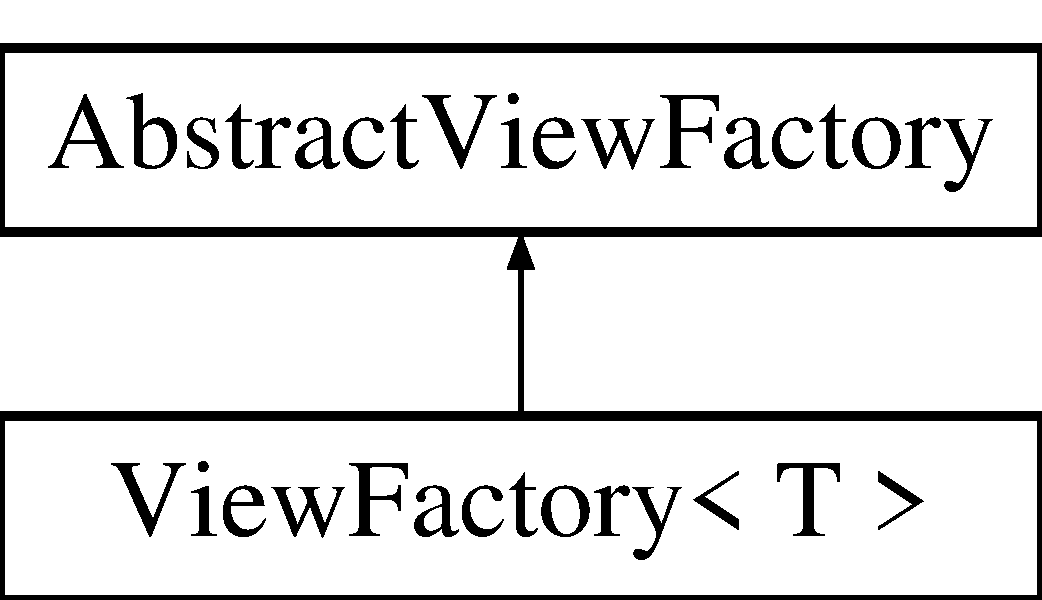
\includegraphics[height=2cm]{class_view_factory}
\end{center}
\end{figure}
\subsection*{Public Member Functions}
\begin{CompactItemize}
\item 
\hypertarget{class_view_factory_fdb0a2655e9918e4fa0b81aeb44109f6}{
virtual boost::shared\_\-ptr$<$ \hyperlink{class_view}{View} $>$ \textbf{create\_\-new\_\-view\_\-instance} (const \hyperlink{class_world_information}{WorldInformation} \&world\_\-information) const }
\label{class_view_factory_fdb0a2655e9918e4fa0b81aeb44109f6}

\end{CompactItemize}


\subsection{Detailed Description}
\subsubsection*{template$<$typename T$>$ class ViewFactory$<$ T $>$}

Interface for a factory which can produce new \hyperlink{class_view}{View} objects.

Factory which can produce new \hyperlink{class_view}{View} objects. The type created is the template type of the factory. 

Definition at line 20 of file view\_\-factory.h.

The documentation for this class was generated from the following file:\begin{CompactItemize}
\item 
src/Views/view\_\-factory.h\end{CompactItemize}

\hypertarget{class_world_information}{
\section{WorldInformation Class Reference}
\label{class_world_information}\index{WorldInformation@{WorldInformation}}
}
Each \hyperlink{class_world_information}{WorldInformation} instance corresponds to the state of the simulated world at a specific simulation step.  


{\tt \#include $<$world\_\-information.h$>$}

\subsection*{Public Member Functions}
\begin{CompactItemize}
\item 
\hypertarget{class_world_information_e0bcb5d40722db2d3f088b8b55b57089}{
\textbf{WorldInformation} (const \hyperlink{class_world_information}{WorldInformation} \&rhs)}
\label{class_world_information_e0bcb5d40722db2d3f088b8b55b57089}

\item 
const vector$<$ boost::shared\_\-ptr$<$ \hyperlink{class_world_object}{WorldObject} $>$ $>$ \& \hyperlink{class_world_information_de860e59ff258afc303720a171d1897e}{markers} () const 
\item 
vector$<$ boost::shared\_\-ptr$<$ \hyperlink{class_world_object}{WorldObject} $>$ $>$ \& \hyperlink{class_world_information_cff2c5c68d7c4dd999c462a0539eb2b2}{markers} ()
\item 
void \hyperlink{class_world_information_1da471aab9fcd304a6913b5b3568c66b}{add\_\-marker} (boost::shared\_\-ptr$<$ \hyperlink{class_world_object}{WorldObject} $>$ new\_\-marker)
\item 
const vector$<$ boost::shared\_\-ptr$<$ Obstacle $>$ $>$ \& \hyperlink{class_world_information_de0421ba8140ec32f9c6be1ced83658d}{obstacles} () const 
\item 
vector$<$ boost::shared\_\-ptr$<$ Obstacle $>$ $>$ \& \hyperlink{class_world_information_3493426dec99ed41f744a2778f8389c2}{obstacles} ()
\item 
void \hyperlink{class_world_information_315a7caced0da0ce9cb10d5db343c541}{add\_\-obstacle} (boost::shared\_\-ptr$<$ Obstacle $>$ new\_\-obstacle)
\item 
const vector$<$ boost::shared\_\-ptr$<$ \hyperlink{class_robot_data}{RobotData} $>$ $>$ \& \hyperlink{class_world_information_349f45bc117c0c25fb0d68dad8af1917}{robot\_\-data} () const 
\item 
vector$<$ boost::shared\_\-ptr$<$ \hyperlink{class_robot_data}{RobotData} $>$ $>$ \& \hyperlink{class_world_information_a4a03f11d75d6a9c036222c58733d1ab}{robot\_\-data} ()
\item 
void \hyperlink{class_world_information_1772ce91751ea42cb9ecdd23c697089a}{add\_\-robot\_\-data} (boost::shared\_\-ptr$<$ \hyperlink{class_robot_data}{RobotData} $>$ new\_\-robot\_\-data)
\item 
int \hyperlink{class_world_information_a20e784bfc5405883fa99313de3137ac}{time} () const 
\item 
void \hyperlink{class_world_information_1e733394b8c0c00d6c6f8ffca95a95e2}{set\_\-time} (int time)
\item 
const \hyperlink{class_robot_data}{RobotData} \& \hyperlink{class_world_information_4815e968feab5c7f034bf97cb96a40b8}{get\_\-according\_\-robot\_\-data} (boost::shared\_\-ptr$<$ \hyperlink{class_robot_identifier}{RobotIdentifier} $>$ id) const 
\item 
\hyperlink{class_robot_data}{RobotData} \& \hyperlink{class_world_information_6efbe4425124ac22c322bcdb3aa2c8a0}{get\_\-according\_\-robot\_\-data} (boost::shared\_\-ptr$<$ \hyperlink{class_robot_identifier}{RobotIdentifier} $>$ id)
\end{CompactItemize}
\subsection*{Private Attributes}
\begin{CompactItemize}
\item 
std::vector$<$ boost::shared\_\-ptr$<$ \hyperlink{class_world_object}{WorldObject} $>$ $>$ \hyperlink{class_world_information_d6fdbbedac7073bf4ae6ca86594e6853}{markers\_\-}
\item 
std::vector$<$ boost::shared\_\-ptr$<$ Obstacle $>$ $>$ \hyperlink{class_world_information_0c5a0ac3fe3570a87495d5dd8c925e27}{obstacles\_\-}
\item 
std::vector$<$ boost::shared\_\-ptr$<$ \hyperlink{class_robot_data}{RobotData} $>$ $>$ \hyperlink{class_world_information_118f01f046eda522ff0b86bc3d5a712d}{robot\_\-data\_\-}
\item 
int \hyperlink{class_world_information_540835d7e7a2311dd77a405655f0bdb4}{time\_\-}
\end{CompactItemize}


\subsection{Detailed Description}
Each \hyperlink{class_world_information}{WorldInformation} instance corresponds to the state of the simulated world at a specific simulation step. 

This class encapsulates information (as e.g. robot position, obstacles, ...) about the simulated world.

Note that this class provides 'const' as well as 'non-const' access most of its data members. In fact, one can think of it more as a struct than a class; the only possibly complex logic may be situated inside the more complex acccessor methods like 'get\_\-according\_\-robot\_\-data'. The 'non-const' access is needed in the \hyperlink{class_event_handler}{EventHandler} to handle \hyperlink{class_request}{Request} for a given robot. After the \hyperlink{class_world_information}{WorldInformation} leaves the \hyperlink{class_event_handler}{EventHandler} only constant references/pointers to it will be accessible.

\begin{Desc}
\item[Author:]Martina Hüllmann \end{Desc}


Definition at line 33 of file world\_\-information.h.

\subsection{Member Function Documentation}
\hypertarget{class_world_information_de860e59ff258afc303720a171d1897e}{
\index{WorldInformation@{WorldInformation}!markers@{markers}}
\index{markers@{markers}!WorldInformation@{WorldInformation}}
\subsubsection[markers]{\setlength{\rightskip}{0pt plus 5cm}const vector$<$ boost::shared\_\-ptr$<$ {\bf WorldObject} $>$ $>$ \& WorldInformation::markers () const}}
\label{class_world_information_de860e59ff258afc303720a171d1897e}


Returns a constant reference to the set of the markers. \begin{Desc}
\item[Returns:]Constant reference to the set of the markers. \end{Desc}


Definition at line 52 of file world\_\-information.cc.

References markers\_\-.

Referenced by EventHandler::extrapolate\_\-old\_\-world\_\-information(), SphericView::init(), and OctreeView::init().\hypertarget{class_world_information_cff2c5c68d7c4dd999c462a0539eb2b2}{
\index{WorldInformation@{WorldInformation}!markers@{markers}}
\index{markers@{markers}!WorldInformation@{WorldInformation}}
\subsubsection[markers]{\setlength{\rightskip}{0pt plus 5cm}vector$<$ boost::shared\_\-ptr$<$ {\bf WorldObject} $>$ $>$ \& WorldInformation::markers ()}}
\label{class_world_information_cff2c5c68d7c4dd999c462a0539eb2b2}


Returns a (non-constant) reference to the set of markers. \begin{Desc}
\item[Returns:]reference to the set of markers. \end{Desc}


Definition at line 56 of file world\_\-information.cc.

References markers\_\-.\hypertarget{class_world_information_1da471aab9fcd304a6913b5b3568c66b}{
\index{WorldInformation@{WorldInformation}!add\_\-marker@{add\_\-marker}}
\index{add\_\-marker@{add\_\-marker}!WorldInformation@{WorldInformation}}
\subsubsection[add\_\-marker]{\setlength{\rightskip}{0pt plus 5cm}void WorldInformation::add\_\-marker (boost::shared\_\-ptr$<$ {\bf WorldObject} $>$ {\em new\_\-marker})}}
\label{class_world_information_1da471aab9fcd304a6913b5b3568c66b}


Adds a new marker to the world. \begin{Desc}
\item[Parameters:]
\begin{description}
\item[{\em Shared}]pointer to the new marker. \end{description}
\end{Desc}


Definition at line 60 of file world\_\-information.cc.

References markers\_\-.\hypertarget{class_world_information_de0421ba8140ec32f9c6be1ced83658d}{
\index{WorldInformation@{WorldInformation}!obstacles@{obstacles}}
\index{obstacles@{obstacles}!WorldInformation@{WorldInformation}}
\subsubsection[obstacles]{\setlength{\rightskip}{0pt plus 5cm}const vector$<$ boost::shared\_\-ptr$<$ Obstacle $>$ $>$ \& WorldInformation::obstacles () const}}
\label{class_world_information_de0421ba8140ec32f9c6be1ced83658d}


Returns a constant reference to the set of the obstacles. \begin{Desc}
\item[Returns:]Constant reference to the set of the obstacles. \end{Desc}


Definition at line 64 of file world\_\-information.cc.

References obstacles\_\-.

Referenced by EventHandler::extrapolate\_\-old\_\-world\_\-information(), SphericView::init(), and OctreeView::init().\hypertarget{class_world_information_3493426dec99ed41f744a2778f8389c2}{
\index{WorldInformation@{WorldInformation}!obstacles@{obstacles}}
\index{obstacles@{obstacles}!WorldInformation@{WorldInformation}}
\subsubsection[obstacles]{\setlength{\rightskip}{0pt plus 5cm}vector$<$ boost::shared\_\-ptr$<$ Obstacle $>$ $>$ \& WorldInformation::obstacles ()}}
\label{class_world_information_3493426dec99ed41f744a2778f8389c2}


Returns a (non-constant) reference to the set of obstacles. \begin{Desc}
\item[Returns:]reference to the set of obstacles. \end{Desc}


Definition at line 68 of file world\_\-information.cc.

References obstacles\_\-.\hypertarget{class_world_information_315a7caced0da0ce9cb10d5db343c541}{
\index{WorldInformation@{WorldInformation}!add\_\-obstacle@{add\_\-obstacle}}
\index{add\_\-obstacle@{add\_\-obstacle}!WorldInformation@{WorldInformation}}
\subsubsection[add\_\-obstacle]{\setlength{\rightskip}{0pt plus 5cm}void WorldInformation::add\_\-obstacle (boost::shared\_\-ptr$<$ Obstacle $>$ {\em new\_\-obstacle})}}
\label{class_world_information_315a7caced0da0ce9cb10d5db343c541}


Adds a new obstacle to the world. \begin{Desc}
\item[Parameters:]
\begin{description}
\item[{\em Shared}]pointer to the new obstacle. \end{description}
\end{Desc}


Definition at line 72 of file world\_\-information.cc.

References obstacles\_\-.\hypertarget{class_world_information_349f45bc117c0c25fb0d68dad8af1917}{
\index{WorldInformation@{WorldInformation}!robot\_\-data@{robot\_\-data}}
\index{robot\_\-data@{robot\_\-data}!WorldInformation@{WorldInformation}}
\subsubsection[robot\_\-data]{\setlength{\rightskip}{0pt plus 5cm}const vector$<$ boost::shared\_\-ptr$<$ {\bf RobotData} $>$ $>$ \& WorldInformation::robot\_\-data () const}}
\label{class_world_information_349f45bc117c0c25fb0d68dad8af1917}


Returns a constant reference to the set of the robot data. \begin{Desc}
\item[Returns:]Constant reference to the set of the robots data. \end{Desc}


Definition at line 76 of file world\_\-information.cc.

References robot\_\-data\_\-.

Referenced by EventHandler::extrapolate\_\-old\_\-world\_\-information(), SphericView::init(), and OctreeView::init().\hypertarget{class_world_information_a4a03f11d75d6a9c036222c58733d1ab}{
\index{WorldInformation@{WorldInformation}!robot\_\-data@{robot\_\-data}}
\index{robot\_\-data@{robot\_\-data}!WorldInformation@{WorldInformation}}
\subsubsection[robot\_\-data]{\setlength{\rightskip}{0pt plus 5cm}vector$<$ boost::shared\_\-ptr$<$ {\bf RobotData} $>$ $>$ \& WorldInformation::robot\_\-data ()}}
\label{class_world_information_a4a03f11d75d6a9c036222c58733d1ab}


Returns a (non-constant) reference to the set of robot data. \begin{Desc}
\item[Returns:]reference to the set of robot data. \end{Desc}


Definition at line 80 of file world\_\-information.cc.

References robot\_\-data\_\-.\hypertarget{class_world_information_1772ce91751ea42cb9ecdd23c697089a}{
\index{WorldInformation@{WorldInformation}!add\_\-robot\_\-data@{add\_\-robot\_\-data}}
\index{add\_\-robot\_\-data@{add\_\-robot\_\-data}!WorldInformation@{WorldInformation}}
\subsubsection[add\_\-robot\_\-data]{\setlength{\rightskip}{0pt plus 5cm}void WorldInformation::add\_\-robot\_\-data (boost::shared\_\-ptr$<$ {\bf RobotData} $>$ {\em new\_\-robot\_\-data})}}
\label{class_world_information_1772ce91751ea42cb9ecdd23c697089a}


Adds a new robot data to the world. \begin{Desc}
\item[Parameters:]
\begin{description}
\item[{\em Shared}]pointer to the new robot data. \end{description}
\end{Desc}


Definition at line 84 of file world\_\-information.cc.

References robot\_\-data\_\-.\hypertarget{class_world_information_a20e784bfc5405883fa99313de3137ac}{
\index{WorldInformation@{WorldInformation}!time@{time}}
\index{time@{time}!WorldInformation@{WorldInformation}}
\subsubsection[time]{\setlength{\rightskip}{0pt plus 5cm}int WorldInformation::time () const}}
\label{class_world_information_a20e784bfc5405883fa99313de3137ac}


Returns the time (measured in steps) when this world info object was created. \begin{Desc}
\item[Returns:]Time (measured in steps) when this world info object was created. \end{Desc}


Definition at line 88 of file world\_\-information.cc.

References time\_\-.

Referenced by EventHandler::extrapolate\_\-old\_\-world\_\-information().\hypertarget{class_world_information_1e733394b8c0c00d6c6f8ffca95a95e2}{
\index{WorldInformation@{WorldInformation}!set\_\-time@{set\_\-time}}
\index{set\_\-time@{set\_\-time}!WorldInformation@{WorldInformation}}
\subsubsection[set\_\-time]{\setlength{\rightskip}{0pt plus 5cm}void WorldInformation::set\_\-time (int {\em time})\hspace{0.3cm}{\tt  \mbox{[}inline\mbox{]}}}}
\label{class_world_information_1e733394b8c0c00d6c6f8ffca95a95e2}


Setter for the time variable \begin{Desc}
\item[Parameters:]
\begin{description}
\item[{\em the}]new time \end{description}
\end{Desc}


Definition at line 107 of file world\_\-information.h.

References time\_\-.\hypertarget{class_world_information_4815e968feab5c7f034bf97cb96a40b8}{
\index{WorldInformation@{WorldInformation}!get\_\-according\_\-robot\_\-data@{get\_\-according\_\-robot\_\-data}}
\index{get\_\-according\_\-robot\_\-data@{get\_\-according\_\-robot\_\-data}!WorldInformation@{WorldInformation}}
\subsubsection[get\_\-according\_\-robot\_\-data]{\setlength{\rightskip}{0pt plus 5cm}const {\bf RobotData} \& WorldInformation::get\_\-according\_\-robot\_\-data (boost::shared\_\-ptr$<$ {\bf RobotIdentifier} $>$ {\em id}) const}}
\label{class_world_information_4815e968feab5c7f034bf97cb96a40b8}


Return constant reference to according robotData of given robot ID

This method assumes, that the according reference to the robotData of a robot with ID i is saved at position i in the robot\_\-datas-vector.

\begin{Desc}
\item[Parameters:]
\begin{description}
\item[{\em reference}]to identifier of robot whose robotData's reference shall be returned. \end{description}
\end{Desc}
\begin{Desc}
\item[Returns:]Constant reference to according robotData of given robot ID. \end{Desc}


Definition at line 92 of file world\_\-information.cc.

References robot\_\-data\_\-.\hypertarget{class_world_information_6efbe4425124ac22c322bcdb3aa2c8a0}{
\index{WorldInformation@{WorldInformation}!get\_\-according\_\-robot\_\-data@{get\_\-according\_\-robot\_\-data}}
\index{get\_\-according\_\-robot\_\-data@{get\_\-according\_\-robot\_\-data}!WorldInformation@{WorldInformation}}
\subsubsection[get\_\-according\_\-robot\_\-data]{\setlength{\rightskip}{0pt plus 5cm}{\bf RobotData} \& WorldInformation::get\_\-according\_\-robot\_\-data (boost::shared\_\-ptr$<$ {\bf RobotIdentifier} $>$ {\em id})}}
\label{class_world_information_6efbe4425124ac22c322bcdb3aa2c8a0}


Return (non-constant) reference to according robotData of given robot ID.

This method assumes, that the according reference to the robotData of a robot with ID i is saved at position i in the robot\_\-datas-vector.

\begin{Desc}
\item[Parameters:]
\begin{description}
\item[{\em reference}]to identifier of robot whose robotData's reference shall be returned. \end{description}
\end{Desc}
\begin{Desc}
\item[Returns:]Mutable reference to according robotData of given robot ID. \end{Desc}


Definition at line 97 of file world\_\-information.cc.

References robot\_\-data\_\-.

\subsection{Member Data Documentation}
\hypertarget{class_world_information_d6fdbbedac7073bf4ae6ca86594e6853}{
\index{WorldInformation@{WorldInformation}!markers\_\-@{markers\_\-}}
\index{markers\_\-@{markers\_\-}!WorldInformation@{WorldInformation}}
\subsubsection[markers\_\-]{\setlength{\rightskip}{0pt plus 5cm}std::vector$<$ boost::shared\_\-ptr$<${\bf WorldObject}$>$ $>$ {\bf WorldInformation::markers\_\-}\hspace{0.3cm}{\tt  \mbox{[}private\mbox{]}}}}
\label{class_world_information_d6fdbbedac7073bf4ae6ca86594e6853}


Set of markers in the world 

Definition at line 137 of file world\_\-information.h.

Referenced by add\_\-marker(), and markers().\hypertarget{class_world_information_0c5a0ac3fe3570a87495d5dd8c925e27}{
\index{WorldInformation@{WorldInformation}!obstacles\_\-@{obstacles\_\-}}
\index{obstacles\_\-@{obstacles\_\-}!WorldInformation@{WorldInformation}}
\subsubsection[obstacles\_\-]{\setlength{\rightskip}{0pt plus 5cm}std::vector$<$ boost::shared\_\-ptr$<$Obstacle$>$ $>$ {\bf WorldInformation::obstacles\_\-}\hspace{0.3cm}{\tt  \mbox{[}private\mbox{]}}}}
\label{class_world_information_0c5a0ac3fe3570a87495d5dd8c925e27}


Set of obstacles in the world 

Definition at line 142 of file world\_\-information.h.

Referenced by add\_\-obstacle(), and obstacles().\hypertarget{class_world_information_118f01f046eda522ff0b86bc3d5a712d}{
\index{WorldInformation@{WorldInformation}!robot\_\-data\_\-@{robot\_\-data\_\-}}
\index{robot\_\-data\_\-@{robot\_\-data\_\-}!WorldInformation@{WorldInformation}}
\subsubsection[robot\_\-data\_\-]{\setlength{\rightskip}{0pt plus 5cm}std::vector$<$ boost::shared\_\-ptr$<${\bf RobotData}$>$ $>$ {\bf WorldInformation::robot\_\-data\_\-}\hspace{0.3cm}{\tt  \mbox{[}private\mbox{]}}}}
\label{class_world_information_118f01f046eda522ff0b86bc3d5a712d}


Set of robot datas of robots in the world 

Definition at line 147 of file world\_\-information.h.

Referenced by add\_\-robot\_\-data(), get\_\-according\_\-robot\_\-data(), and robot\_\-data().\hypertarget{class_world_information_540835d7e7a2311dd77a405655f0bdb4}{
\index{WorldInformation@{WorldInformation}!time\_\-@{time\_\-}}
\index{time\_\-@{time\_\-}!WorldInformation@{WorldInformation}}
\subsubsection[time\_\-]{\setlength{\rightskip}{0pt plus 5cm}int {\bf WorldInformation::time\_\-}\hspace{0.3cm}{\tt  \mbox{[}private\mbox{]}}}}
\label{class_world_information_540835d7e7a2311dd77a405655f0bdb4}


Time (measured in steps) of creation of this world information 

Definition at line 152 of file world\_\-information.h.

Referenced by set\_\-time(), and time().

The documentation for this class was generated from the following files:\begin{CompactItemize}
\item 
src/Model/world\_\-information.h\item 
src/Model/world\_\-information.cc\end{CompactItemize}

\hypertarget{class_world_object}{
\section{WorldObject Class Reference}
\label{class_world_object}\index{WorldObject@{WorldObject}}
}
Denotes an obstacle in the world.  


{\tt \#include $<$obstacle.h$>$}

Inheritance diagram for WorldObject::\begin{figure}[H]
\begin{center}
\leavevmode
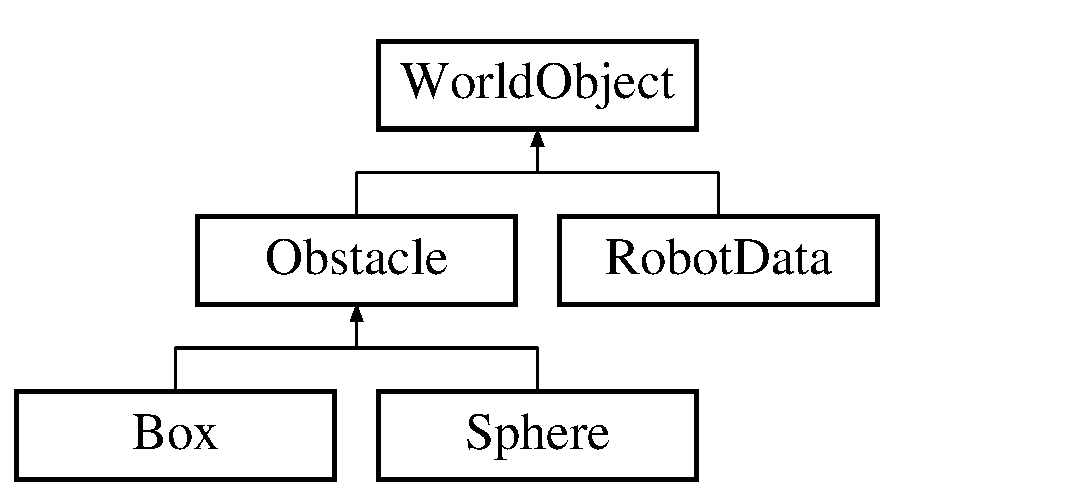
\includegraphics[height=3cm]{class_world_object}
\end{center}
\end{figure}
\subsection*{Public Member Functions}
\begin{CompactItemize}
\item 
\hypertarget{class_world_object_7bd53cd60f7d36d5ce95d47eaed9f835}{
\textbf{WorldObject} (boost::shared\_\-ptr$<$ \hyperlink{class_identifier}{Identifier} $>$ id, boost::shared\_\-ptr$<$ Vector3d $>$ position, boost::shared\_\-ptr$<$ \hyperlink{class_marker_information}{MarkerInformation} $>$ marker\_\-information=boost::shared\_\-ptr$<$ \hyperlink{class_marker_information}{MarkerInformation} $>$(new \hyperlink{class_marker_information}{MarkerInformation}()))}
\label{class_world_object_7bd53cd60f7d36d5ce95d47eaed9f835}

\item 
\hypertarget{class_world_object_057d73f35e0574e1f8e8f1437cdaaa25}{
\textbf{WorldObject} (const \hyperlink{class_world_object}{WorldObject} \&rhs)}
\label{class_world_object_057d73f35e0574e1f8e8f1437cdaaa25}

\item 
void \hyperlink{class_world_object_a502586bf3c68894552f805cd6b99670}{set\_\-marker\_\-information} (boost::shared\_\-ptr$<$ \hyperlink{class_marker_information}{MarkerInformation} $>$ new\_\-marker\_\-information)
\item 
const \hyperlink{class_marker_information}{MarkerInformation} \& \hyperlink{class_world_object_1dd7d80498c6b502ad9870c54cbf4305}{marker\_\-information} () const 
\item 
void \hyperlink{class_world_object_60afe09f64b069c79833bb9a07a71cc1}{set\_\-position} (boost::shared\_\-ptr$<$ Vector3d $>$ new\_\-position)
\item 
const Vector3d \& \hyperlink{class_world_object_27b52dcd1b64d4dd45936da833e1ea26}{position} () const 
\item 
const boost::shared\_\-ptr$<$ \hyperlink{class_identifier}{Identifier} $>$ \& \hyperlink{class_world_object_86cb6d16f21d52ebe8f9dc48e9e762f3}{id} () const 
\item 
virtual boost::shared\_\-ptr$<$ \hyperlink{class_world_object}{WorldObject} $>$ \hyperlink{class_world_object_dba468299ce77ce5781e60081bf44b14}{clone} () const 
\end{CompactItemize}
\subsection*{Protected Attributes}
\begin{CompactItemize}
\item 
boost::shared\_\-ptr$<$ Vector3d $>$ \hyperlink{class_world_object_f445cb9e3a29647e35064a14ae458b78}{position\_\-}
\end{CompactItemize}
\subsection*{Private Attributes}
\begin{CompactItemize}
\item 
\hypertarget{class_world_object_4f3fb32c00469db5b5ed9c4622f9ddcb}{
boost::shared\_\-ptr$<$ \hyperlink{class_identifier}{Identifier} $>$ \textbf{id\_\-}}
\label{class_world_object_4f3fb32c00469db5b5ed9c4622f9ddcb}

\item 
boost::shared\_\-ptr$<$ \hyperlink{class_marker_information}{MarkerInformation} $>$ \hyperlink{class_world_object_837a1b5d6014ae2265d8d6f9caf65754}{marker\_\-information\_\-}
\end{CompactItemize}


\subsection{Detailed Description}
Denotes an obstacle in the world. 

An instance of this class denotes an object (robot, marker, obstacle) in the world.

\begin{Desc}
\item[Author:]Martina Hüllmann \end{Desc}


Definition at line 16 of file world\_\-object.h.

\subsection{Member Function Documentation}
\hypertarget{class_world_object_a502586bf3c68894552f805cd6b99670}{
\index{WorldObject@{WorldObject}!set\_\-marker\_\-information@{set\_\-marker\_\-information}}
\index{set\_\-marker\_\-information@{set\_\-marker\_\-information}!WorldObject@{WorldObject}}
\subsubsection[set\_\-marker\_\-information]{\setlength{\rightskip}{0pt plus 5cm}void WorldObject::set\_\-marker\_\-information (boost::shared\_\-ptr$<$ {\bf MarkerInformation} $>$ {\em new\_\-marker\_\-information})}}
\label{class_world_object_a502586bf3c68894552f805cd6b99670}


Sets the marker information of this object. \begin{Desc}
\item[Parameters:]
\begin{description}
\item[{\em a}]shared pointer to the new marker information \end{description}
\end{Desc}


Definition at line 33 of file world\_\-object.cc.

References marker\_\-information\_\-.\hypertarget{class_world_object_1dd7d80498c6b502ad9870c54cbf4305}{
\index{WorldObject@{WorldObject}!marker\_\-information@{marker\_\-information}}
\index{marker\_\-information@{marker\_\-information}!WorldObject@{WorldObject}}
\subsubsection[marker\_\-information]{\setlength{\rightskip}{0pt plus 5cm}const {\bf MarkerInformation} \& WorldObject::marker\_\-information () const}}
\label{class_world_object_1dd7d80498c6b502ad9870c54cbf4305}


Returns a constant reference to the marker information of this object. \begin{Desc}
\item[Returns:]Constant reference to the marker information of this object. \end{Desc}


Definition at line 29 of file world\_\-object.cc.

References marker\_\-information\_\-.\hypertarget{class_world_object_60afe09f64b069c79833bb9a07a71cc1}{
\index{WorldObject@{WorldObject}!set\_\-position@{set\_\-position}}
\index{set\_\-position@{set\_\-position}!WorldObject@{WorldObject}}
\subsubsection[set\_\-position]{\setlength{\rightskip}{0pt plus 5cm}void WorldObject::set\_\-position (boost::shared\_\-ptr$<$ Vector3d $>$ {\em new\_\-position})\hspace{0.3cm}{\tt  \mbox{[}inline\mbox{]}}}}
\label{class_world_object_60afe09f64b069c79833bb9a07a71cc1}


Sets the position of this object. \begin{Desc}
\item[Parameters:]
\begin{description}
\item[{\em Pointer}]to new position vector. \end{description}
\end{Desc}


Definition at line 40 of file world\_\-object.h.

References position\_\-.\hypertarget{class_world_object_27b52dcd1b64d4dd45936da833e1ea26}{
\index{WorldObject@{WorldObject}!position@{position}}
\index{position@{position}!WorldObject@{WorldObject}}
\subsubsection[position]{\setlength{\rightskip}{0pt plus 5cm}const Vector3d\& WorldObject::position () const\hspace{0.3cm}{\tt  \mbox{[}inline\mbox{]}}}}
\label{class_world_object_27b52dcd1b64d4dd45936da833e1ea26}


Returns constant reference to position vector. \begin{Desc}
\item[Returns:]Constant reference to position vector. \end{Desc}


Definition at line 46 of file world\_\-object.h.

References position\_\-.

Referenced by RobotData::extrapolated\_\-position().\hypertarget{class_world_object_86cb6d16f21d52ebe8f9dc48e9e762f3}{
\index{WorldObject@{WorldObject}!id@{id}}
\index{id@{id}!WorldObject@{WorldObject}}
\subsubsection[id]{\setlength{\rightskip}{0pt plus 5cm}const boost::shared\_\-ptr$<$ {\bf Identifier} $>$ \& WorldObject::id () const}}
\label{class_world_object_86cb6d16f21d52ebe8f9dc48e9e762f3}


Returns constant reference to the object's id. \begin{Desc}
\item[Returns:]Constant reference to the object's id. \end{Desc}


Definition at line 37 of file world\_\-object.cc.\hypertarget{class_world_object_dba468299ce77ce5781e60081bf44b14}{
\index{WorldObject@{WorldObject}!clone@{clone}}
\index{clone@{clone}!WorldObject@{WorldObject}}
\subsubsection[clone]{\setlength{\rightskip}{0pt plus 5cm}boost::shared\_\-ptr$<$ {\bf WorldObject} $>$ WorldObject::clone () const\hspace{0.3cm}{\tt  \mbox{[}virtual\mbox{]}}}}
\label{class_world_object_dba468299ce77ce5781e60081bf44b14}


Clones this object and returns a shared ptr to the cloned object. typeid($\ast$this) == typeid($\ast$clone) \begin{Desc}
\item[Returns:]shared ptr to the cloned object \end{Desc}


Reimplemented in \hyperlink{class_box_06c27f9a07a6ba9e87aa0c2e57237b5c}{Box}, \hyperlink{class_robot_data_81b5c3ba1f959f41ff3a9cb8067d75cb}{RobotData}, and \hyperlink{class_sphere_6fcc846dbbef396057b572b9a0786cdc}{Sphere}.

Definition at line 41 of file world\_\-object.cc.

\subsection{Member Data Documentation}
\hypertarget{class_world_object_f445cb9e3a29647e35064a14ae458b78}{
\index{WorldObject@{WorldObject}!position\_\-@{position\_\-}}
\index{position\_\-@{position\_\-}!WorldObject@{WorldObject}}
\subsubsection[position\_\-]{\setlength{\rightskip}{0pt plus 5cm}boost::shared\_\-ptr$<$Vector3d$>$ {\bf WorldObject::position\_\-}\hspace{0.3cm}{\tt  \mbox{[}protected\mbox{]}}}}
\label{class_world_object_f445cb9e3a29647e35064a14ae458b78}


Position of the world object in the world. This point always is the point in the center of the object 

Definition at line 68 of file world\_\-object.h.

Referenced by position(), and set\_\-position().\hypertarget{class_world_object_837a1b5d6014ae2265d8d6f9caf65754}{
\index{WorldObject@{WorldObject}!marker\_\-information\_\-@{marker\_\-information\_\-}}
\index{marker\_\-information\_\-@{marker\_\-information\_\-}!WorldObject@{WorldObject}}
\subsubsection[marker\_\-information\_\-]{\setlength{\rightskip}{0pt plus 5cm}boost::shared\_\-ptr$<${\bf MarkerInformation}$>$ {\bf WorldObject::marker\_\-information\_\-}\hspace{0.3cm}{\tt  \mbox{[}private\mbox{]}}}}
\label{class_world_object_837a1b5d6014ae2265d8d6f9caf65754}


Information about the marker an instance of \hyperlink{class_world_object}{WorldObject} may contain 

Definition at line 73 of file world\_\-object.h.

Referenced by marker\_\-information(), and set\_\-marker\_\-information().

The documentation for this class was generated from the following files:\begin{CompactItemize}
\item 
src/Model/world\_\-object.h\item 
src/Model/world\_\-object.cc\end{CompactItemize}

\printindex
\end{document}
